\documentclass[a4paper]{book}
\usepackage{a4wide}
\usepackage{makeidx}
\usepackage{graphicx}
\usepackage{multicol}
\usepackage{float}
\usepackage{listings}
\usepackage{color}
\usepackage{textcomp}
\usepackage{alltt}
\usepackage{times}
\usepackage{ifpdf}
\ifpdf
\usepackage[pdftex,
            pagebackref=true,
            colorlinks=true,
            linkcolor=blue,
            unicode
           ]{hyperref}
\else
\usepackage[ps2pdf,
            pagebackref=true,
            colorlinks=true,
            linkcolor=blue,
            unicode
           ]{hyperref}
\usepackage{pspicture}
\fi
\usepackage[utf8]{inputenc}
\usepackage{doxygen}
\lstset{language=C++,inputencoding=utf8,basicstyle=\footnotesize,breaklines=true,breakatwhitespace=true,tabsize=8,numbers=left }
\makeindex
\setcounter{tocdepth}{3}
\renewcommand{\footrulewidth}{0.4pt}
\begin{document}
\hypersetup{pageanchor=false}
\begin{titlepage}
\vspace*{7cm}
\begin{center}
{\Large crml \\[1ex]\large .1 }\\
\vspace*{1cm}
{\large Generated by Doxygen 1.6.3}\\
\vspace*{0.5cm}
{\small Thu Nov 4 13:14:12 2010}\\
\end{center}
\end{titlepage}
\clearemptydoublepage
\pagenumbering{roman}
\tableofcontents
\clearemptydoublepage
\pagenumbering{arabic}
\hypersetup{pageanchor=true}
\chapter{Namespace Index}
\section{Namespace List}
Here is a list of all namespaces with brief descriptions:\begin{DoxyCompactList}
\item\contentsline{section}{\hyperlink{namespacebridge}{bridge} }{\pageref{namespacebridge}}{}
\item\contentsline{section}{\hyperlink{namespacecpplint}{cpplint} }{\pageref{namespacecpplint}}{}
\item\contentsline{section}{\hyperlink{namespacecrml}{crml} }{\pageref{namespacecrml}}{}
\item\contentsline{section}{\hyperlink{namespacehexdecode}{hexdecode} }{\pageref{namespacehexdecode}}{}
\item\contentsline{section}{\hyperlink{namespacehexencode}{hexencode} }{\pageref{namespacehexencode}}{}
\item\contentsline{section}{\hyperlink{namespacehexjs}{hexjs} }{\pageref{namespacehexjs}}{}
\item\contentsline{section}{\hyperlink{namespacehttpd}{httpd} }{\pageref{namespacehttpd}}{}
\item\contentsline{section}{\hyperlink{namespacepi__generator}{pi\_\-generator} }{\pageref{namespacepi__generator}}{}
\item\contentsline{section}{\hyperlink{namespacepp}{pp} }{\pageref{namespacepp}}{}
\item\contentsline{section}{\hyperlink{namespacescm}{scm} }{\pageref{namespacescm}}{}
\item\contentsline{section}{\hyperlink{namespaceshader__util}{shader\_\-util} }{\pageref{namespaceshader__util}}{}
\item\contentsline{section}{\hyperlink{namespacetransform__4x4}{transform\_\-4x4} }{\pageref{namespacetransform__4x4}}{}
\item\contentsline{section}{\hyperlink{namespacetumbler}{tumbler} }{\pageref{namespacetumbler}}{}
\end{DoxyCompactList}

\chapter{Class Index}
\section{Class Hierarchy}
This inheritance list is sorted roughly, but not completely, alphabetically:\begin{DoxyCompactList}
\item \contentsline{section}{scm::Clock}{\pageref{classscm_1_1_clock}}{}
\item \contentsline{section}{Context}{\pageref{struct_context}}{}
\item \contentsline{section}{crml::Core}{\pageref{classcrml_1_1_core}}{}
\item \contentsline{section}{tumbler::Cube}{\pageref{classtumbler_1_1_cube}}{}
\item \contentsline{section}{crml::Display}{\pageref{classcrml_1_1_display}}{}
\item \contentsline{section}{scm::Error}{\pageref{classscm_1_1_error}}{}
\begin{DoxyCompactList}
\item \contentsline{section}{scm::Event}{\pageref{classscm_1_1_event}}{}
\end{DoxyCompactList}
\item \contentsline{section}{EventHandler}{\pageref{class_event_handler}}{}
\item \contentsline{section}{HelloWorldInstance}{\pageref{class_hello_world_instance}}{}
\item \contentsline{section}{HelloWorldModule}{\pageref{class_hello_world_module}}{}
\item \contentsline{section}{HelloWorldScriptableObject}{\pageref{class_hello_world_scriptable_object}}{}
\item \contentsline{section}{scm::HexStore}{\pageref{classscm_1_1_hex_store}}{}
\item \contentsline{section}{MD5Digest\_\-struct}{\pageref{struct_m_d5_digest__struct}}{}
\item \contentsline{section}{pi\_\-generator::PiGenerator}{\pageref{classpi__generator_1_1_pi_generator}}{}
\item \contentsline{section}{httpd::QuittableHTTPHandler}{\pageref{classhttpd_1_1_quittable_h_t_t_p_handler}}{}
\item \contentsline{section}{httpd::QuittableHTTPServer}{\pageref{classhttpd_1_1_quittable_h_t_t_p_server}}{}
\item \contentsline{section}{ScriptingBridge}{\pageref{class_scripting_bridge}}{}
\item \contentsline{section}{bridge::ScriptingBridge}{\pageref{classbridge_1_1_scripting_bridge}}{}
\begin{DoxyCompactList}
\item \contentsline{section}{bridge::PiGenerator}{\pageref{classbridge_1_1_pi_generator}}{}
\end{DoxyCompactList}
\item \contentsline{section}{tumbler::ScriptingBridge}{\pageref{classtumbler_1_1_scripting_bridge}}{}
\item \contentsline{section}{pi\_\-generator::ScriptingBridge}{\pageref{classpi__generator_1_1_scripting_bridge}}{}
\item \contentsline{section}{TestObject}{\pageref{struct_test_object}}{}
\item \contentsline{section}{tumbler::Tumbler}{\pageref{classtumbler_1_1_tumbler}}{}
\item \contentsline{section}{tumbler::TumblerContext3D}{\pageref{structtumbler_1_1_tumbler_context3_d}}{}
\end{DoxyCompactList}

\chapter{Class Index}
\section{Class List}
Here are the classes, structs, unions and interfaces with brief descriptions:\begin{DoxyCompactList}
\item\contentsline{section}{\hyperlink{classscm_1_1_clock}{scm::Clock} }{\pageref{classscm_1_1_clock}}{}
\item\contentsline{section}{\hyperlink{struct_context}{Context} }{\pageref{struct_context}}{}
\item\contentsline{section}{\hyperlink{classcrml_1_1_core}{crml::Core} (The \hyperlink{classcrml_1_1_core}{Core} object which wires all subsystems and maintains an open channel with javascript )}{\pageref{classcrml_1_1_core}}{}
\item\contentsline{section}{\hyperlink{classtumbler_1_1_cube}{tumbler::Cube} }{\pageref{classtumbler_1_1_cube}}{}
\item\contentsline{section}{\hyperlink{classcrml_1_1_display}{crml::Display} }{\pageref{classcrml_1_1_display}}{}
\item\contentsline{section}{\hyperlink{classscm_1_1_error}{scm::Error} }{\pageref{classscm_1_1_error}}{}
\item\contentsline{section}{\hyperlink{classscm_1_1_event}{scm::Event} }{\pageref{classscm_1_1_event}}{}
\item\contentsline{section}{\hyperlink{class_event_handler}{EventHandler} }{\pageref{class_event_handler}}{}
\item\contentsline{section}{\hyperlink{class_hello_world_instance}{HelloWorldInstance} }{\pageref{class_hello_world_instance}}{}
\item\contentsline{section}{\hyperlink{class_hello_world_module}{HelloWorldModule} }{\pageref{class_hello_world_module}}{}
\item\contentsline{section}{\hyperlink{class_hello_world_scriptable_object}{HelloWorldScriptableObject} }{\pageref{class_hello_world_scriptable_object}}{}
\item\contentsline{section}{\hyperlink{classscm_1_1_hex_store}{scm::HexStore} }{\pageref{classscm_1_1_hex_store}}{}
\item\contentsline{section}{\hyperlink{struct_m_d5_digest__struct}{MD5Digest\_\-struct} }{\pageref{struct_m_d5_digest__struct}}{}
\item\contentsline{section}{\hyperlink{classbridge_1_1_pi_generator}{bridge::PiGenerator} }{\pageref{classbridge_1_1_pi_generator}}{}
\item\contentsline{section}{\hyperlink{classpi__generator_1_1_pi_generator}{pi\_\-generator::PiGenerator} }{\pageref{classpi__generator_1_1_pi_generator}}{}
\item\contentsline{section}{\hyperlink{classhttpd_1_1_quittable_h_t_t_p_handler}{httpd::QuittableHTTPHandler} }{\pageref{classhttpd_1_1_quittable_h_t_t_p_handler}}{}
\item\contentsline{section}{\hyperlink{classhttpd_1_1_quittable_h_t_t_p_server}{httpd::QuittableHTTPServer} }{\pageref{classhttpd_1_1_quittable_h_t_t_p_server}}{}
\item\contentsline{section}{\hyperlink{class_scripting_bridge}{ScriptingBridge} }{\pageref{class_scripting_bridge}}{}
\item\contentsline{section}{\hyperlink{classbridge_1_1_scripting_bridge}{bridge::ScriptingBridge} }{\pageref{classbridge_1_1_scripting_bridge}}{}
\item\contentsline{section}{\hyperlink{classtumbler_1_1_scripting_bridge}{tumbler::ScriptingBridge} }{\pageref{classtumbler_1_1_scripting_bridge}}{}
\item\contentsline{section}{\hyperlink{classpi__generator_1_1_scripting_bridge}{pi\_\-generator::ScriptingBridge} }{\pageref{classpi__generator_1_1_scripting_bridge}}{}
\item\contentsline{section}{\hyperlink{struct_test_object}{TestObject} }{\pageref{struct_test_object}}{}
\item\contentsline{section}{\hyperlink{classtumbler_1_1_tumbler}{tumbler::Tumbler} }{\pageref{classtumbler_1_1_tumbler}}{}
\item\contentsline{section}{\hyperlink{structtumbler_1_1_tumbler_context3_d}{tumbler::TumblerContext3D} }{\pageref{structtumbler_1_1_tumbler_context3_d}}{}
\end{DoxyCompactList}

\chapter{File Index}
\section{File List}
Here is a list of all files with brief descriptions:\begin{DoxyCompactList}
\item\contentsline{section}{/home/derek/dev/crml/crml/lib/tumbler/\hyperlink{basic__macros_8h}{basic\_\-macros.h} }{\pageref{basic__macros_8h}}{}
\item\contentsline{section}{/home/derek/dev/crml/crml/lib/tumbler/\hyperlink{cube_8cc}{cube.cc} }{\pageref{cube_8cc}}{}
\item\contentsline{section}{/home/derek/dev/crml/crml/lib/tumbler/\hyperlink{cube_8h}{cube.h} }{\pageref{cube_8h}}{}
\item\contentsline{section}{/home/derek/dev/crml/crml/lib/tumbler/\hyperlink{lib_2tumbler_2npn__bridge_8cc}{npn\_\-bridge.cc} }{\pageref{lib_2tumbler_2npn__bridge_8cc}}{}
\item\contentsline{section}{/home/derek/dev/crml/crml/lib/tumbler/\hyperlink{lib_2tumbler_2npp__gate_8cc}{npp\_\-gate.cc} }{\pageref{lib_2tumbler_2npp__gate_8cc}}{}
\item\contentsline{section}{/home/derek/dev/crml/crml/lib/tumbler/\hyperlink{lib_2tumbler_2scripting__bridge_8cc}{scripting\_\-bridge.cc} }{\pageref{lib_2tumbler_2scripting__bridge_8cc}}{}
\item\contentsline{section}{/home/derek/dev/crml/crml/lib/tumbler/\hyperlink{lib_2tumbler_2scripting__bridge_8h}{scripting\_\-bridge.h} }{\pageref{lib_2tumbler_2scripting__bridge_8h}}{}
\item\contentsline{section}{/home/derek/dev/crml/crml/lib/tumbler/\hyperlink{shader__util_8cc}{shader\_\-util.cc} }{\pageref{shader__util_8cc}}{}
\item\contentsline{section}{/home/derek/dev/crml/crml/lib/tumbler/\hyperlink{shader__util_8h}{shader\_\-util.h} }{\pageref{shader__util_8h}}{}
\item\contentsline{section}{/home/derek/dev/crml/crml/lib/tumbler/\hyperlink{transforms_8cc}{transforms.cc} }{\pageref{transforms_8cc}}{}
\item\contentsline{section}{/home/derek/dev/crml/crml/lib/tumbler/\hyperlink{transforms_8h}{transforms.h} }{\pageref{transforms_8h}}{}
\item\contentsline{section}{/home/derek/dev/crml/crml/lib/tumbler/\hyperlink{tumbler_8cc}{tumbler.cc} }{\pageref{tumbler_8cc}}{}
\item\contentsline{section}{/home/derek/dev/crml/crml/lib/tumbler/\hyperlink{tumbler_8h}{tumbler.h} }{\pageref{tumbler_8h}}{}
\item\contentsline{section}{/home/derek/dev/crml/crml/lib/tumbler/\hyperlink{tumbler__module_8cc}{tumbler\_\-module.cc} }{\pageref{tumbler__module_8cc}}{}
\item\contentsline{section}{/home/derek/dev/crml/crml/src/core/\hyperlink{core_8h}{core.h} }{\pageref{core_8h}}{}
\item\contentsline{section}{/home/derek/dev/crml/crml/src/core/\hyperlink{src_2core_2npn__bridge_8cc}{npn\_\-bridge.cc} }{\pageref{src_2core_2npn__bridge_8cc}}{}
\item\contentsline{section}{/home/derek/dev/crml/crml/src/core/\hyperlink{src_2core_2npp__gate_8cc}{npp\_\-gate.cc} }{\pageref{src_2core_2npp__gate_8cc}}{}
\item\contentsline{section}{/home/derek/dev/crml/crml/src/core/\hyperlink{src_2core_2scripting__bridge_8cc}{scripting\_\-bridge.cc} }{\pageref{src_2core_2scripting__bridge_8cc}}{}
\item\contentsline{section}{/home/derek/dev/crml/crml/src/core/\hyperlink{src_2core_2scripting__bridge_8h}{scripting\_\-bridge.h} }{\pageref{src_2core_2scripting__bridge_8h}}{}
\item\contentsline{section}{/home/derek/dev/crml/crml/src/evt/\hyperlink{event_8cc}{event.cc} }{\pageref{event_8cc}}{}
\item\contentsline{section}{/home/derek/dev/crml/crml/src/evt/\hyperlink{event_8h}{event.h} }{\pageref{event_8h}}{}
\item\contentsline{section}{/home/derek/dev/crml/crml/src/evt/\hyperlink{event__handler_8cc}{event\_\-handler.cc} }{\pageref{event__handler_8cc}}{}
\item\contentsline{section}{/home/derek/dev/crml/crml/src/evt/\hyperlink{event__handler_8h}{event\_\-handler.h} }{\pageref{event__handler_8h}}{}
\item\contentsline{section}{/home/derek/dev/crml/crml/src/gfx/\hyperlink{display_8hpp}{display.hpp} }{\pageref{display_8hpp}}{}
\item\contentsline{section}{/home/derek/dev/crml/crml/src/gfx/\hyperlink{gles2__demo__cc_8cc}{gles2\_\-demo\_\-cc.cc} }{\pageref{gles2__demo__cc_8cc}}{}
\item\contentsline{section}{/home/derek/dev/crml/crml/src/gfx/\hyperlink{gles2__demo__cc_8h}{gles2\_\-demo\_\-cc.h} }{\pageref{gles2__demo__cc_8h}}{}
\item\contentsline{section}{/home/derek/dev/crml/crml/src/gfx/\hyperlink{_png_image_8h}{PngImage.h} }{\pageref{_png_image_8h}}{}
\item\contentsline{section}{/home/derek/dev/crml/crml/src/include/\hyperlink{crml-aud_8h}{crml-\/aud.h} }{\pageref{crml-aud_8h}}{}
\item\contentsline{section}{/home/derek/dev/crml/crml/src/include/\hyperlink{crml-core_8h}{crml-\/core.h} }{\pageref{crml-core_8h}}{}
\item\contentsline{section}{/home/derek/dev/crml/crml/src/include/\hyperlink{crml-evt_8h}{crml-\/evt.h} }{\pageref{crml-evt_8h}}{}
\item\contentsline{section}{/home/derek/dev/crml/crml/src/include/\hyperlink{crml-gfx_8h}{crml-\/gfx.h} }{\pageref{crml-gfx_8h}}{}
\item\contentsline{section}{/home/derek/dev/crml/crml/src/include/\hyperlink{crml-net_8h}{crml-\/net.h} }{\pageref{crml-net_8h}}{}
\item\contentsline{section}{/home/derek/dev/crml/crml/src/include/\hyperlink{crml-sys_8h}{crml-\/sys.h} }{\pageref{crml-sys_8h}}{}
\item\contentsline{section}{/home/derek/dev/crml/crml/src/include/\hyperlink{crml-util_8h}{crml-\/util.h} }{\pageref{crml-util_8h}}{}
\item\contentsline{section}{/home/derek/dev/crml/crml/src/include/\hyperlink{crml-web_8h}{crml-\/web.h} }{\pageref{crml-web_8h}}{}
\item\contentsline{section}{/home/derek/dev/crml/crml/src/include/\hyperlink{crml-win_8h}{crml-\/win.h} }{\pageref{crml-win_8h}}{}
\item\contentsline{section}{/home/derek/dev/crml/crml/src/sys/\hyperlink{clock_8cc}{clock.cc} }{\pageref{clock_8cc}}{}
\item\contentsline{section}{/home/derek/dev/crml/crml/src/sys/\hyperlink{clock_8h}{clock.h} }{\pageref{clock_8h}}{}
\item\contentsline{section}{/home/derek/dev/crml/crml/src/sys/\hyperlink{error_8cc}{error.cc} }{\pageref{error_8cc}}{}
\item\contentsline{section}{/home/derek/dev/crml/crml/src/sys/\hyperlink{error_8h}{error.h} }{\pageref{error_8h}}{}
\item\contentsline{section}{/home/derek/dev/crml/crml/src/sys/\hyperlink{error__macro_8cc}{error\_\-macro.cc} }{\pageref{error__macro_8cc}}{}
\item\contentsline{section}{/home/derek/dev/crml/crml/src/sys/\hyperlink{hex__store_8cc}{hex\_\-store.cc} }{\pageref{hex__store_8cc}}{}
\item\contentsline{section}{/home/derek/dev/crml/crml/src/sys/\hyperlink{hex__store_8h}{hex\_\-store.h} }{\pageref{hex__store_8h}}{}
\item\contentsline{section}{/home/derek/dev/crml/crml/src/sys/\hyperlink{hexdecode_8cc}{hexdecode.cc} }{\pageref{hexdecode_8cc}}{}
\item\contentsline{section}{/home/derek/dev/crml/crml/src/sys/\hyperlink{log__macro_8cc}{log\_\-macro.cc} }{\pageref{log__macro_8cc}}{}
\item\contentsline{section}{/home/derek/dev/crml/crml/src/sys/\hyperlink{md5_8cc}{md5.cc} }{\pageref{md5_8cc}}{}
\item\contentsline{section}{/home/derek/dev/crml/crml/src/sys/\hyperlink{md5_8h}{md5.h} }{\pageref{md5_8h}}{}
\item\contentsline{section}{/home/derek/dev/crml/crml/src/sys/\hyperlink{src_2sys_2scripting__bridge_8h}{scripting\_\-bridge.h} }{\pageref{src_2sys_2scripting__bridge_8h}}{}
\item\contentsline{section}{/home/derek/dev/crml/crml/src/sys/tmp/\hyperlink{jslog_8cc}{jslog.cc} }{\pageref{jslog_8cc}}{}
\item\contentsline{section}{/home/derek/dev/crml/crml/src/web/\hyperlink{src_2web_2httpd_8py}{httpd.py} }{\pageref{src_2web_2httpd_8py}}{}
\item\contentsline{section}{/home/derek/dev/crml/crml/test/\hyperlink{hexjs_8py}{hexjs.py} }{\pageref{hexjs_8py}}{}
\item\contentsline{section}{/home/derek/dev/crml/crml/test/\hyperlink{test_2httpd_8py}{httpd.py} }{\pageref{test_2httpd_8py}}{}
\item\contentsline{section}{/home/derek/dev/crml/crml/test/\hyperlink{test-clock_8cc}{test-\/clock.cc} }{\pageref{test-clock_8cc}}{}
\item\contentsline{section}{/home/derek/dev/crml/crml/test/\hyperlink{test-macros_8cc}{test-\/macros.cc} }{\pageref{test-macros_8cc}}{}
\item\contentsline{section}{/home/derek/dev/crml/crml/test/\hyperlink{test-point_8cc}{test-\/point.cc} }{\pageref{test-point_8cc}}{}
\item\contentsline{section}{/home/derek/dev/crml/crml/test/\hyperlink{test__object_8cc}{test\_\-object.cc} }{\pageref{test__object_8cc}}{}
\item\contentsline{section}{/home/derek/dev/crml/crml/test/\hyperlink{test__object_8h}{test\_\-object.h} }{\pageref{test__object_8h}}{}
\item\contentsline{section}{/home/derek/dev/crml/crml/test/crml\_\-hello\_\-world/\hyperlink{test_2crml__hello__world_2npn__bridge_8cc}{npn\_\-bridge.cc} }{\pageref{test_2crml__hello__world_2npn__bridge_8cc}}{}
\item\contentsline{section}{/home/derek/dev/crml/crml/test/crml\_\-hello\_\-world/\hyperlink{test_2crml__hello__world_2npp__gate_8cc}{npp\_\-gate.cc} }{\pageref{test_2crml__hello__world_2npp__gate_8cc}}{}
\item\contentsline{section}{/home/derek/dev/crml/crml/test/crml\_\-hello\_\-world/\hyperlink{crml__hello__world_2pi__generator_8cc}{pi\_\-generator.cc} }{\pageref{crml__hello__world_2pi__generator_8cc}}{}
\item\contentsline{section}{/home/derek/dev/crml/crml/test/crml\_\-hello\_\-world/\hyperlink{crml__hello__world_2pi__generator_8h}{pi\_\-generator.h} }{\pageref{crml__hello__world_2pi__generator_8h}}{}
\item\contentsline{section}{/home/derek/dev/crml/crml/test/crml\_\-hello\_\-world/\hyperlink{crml__hello__world_2pi__generator__module_8cc}{pi\_\-generator\_\-module.cc} }{\pageref{crml__hello__world_2pi__generator__module_8cc}}{}
\item\contentsline{section}{/home/derek/dev/crml/crml/test/crml\_\-hello\_\-world/\hyperlink{test_2crml__hello__world_2scripting__bridge_8cc}{scripting\_\-bridge.cc} }{\pageref{test_2crml__hello__world_2scripting__bridge_8cc}}{}
\item\contentsline{section}{/home/derek/dev/crml/crml/test/crml\_\-hello\_\-world/\hyperlink{test_2crml__hello__world_2scripting__bridge_8h}{scripting\_\-bridge.h} }{\pageref{test_2crml__hello__world_2scripting__bridge_8h}}{}
\item\contentsline{section}{/home/derek/dev/crml/crml/test/hello\_\-world/\hyperlink{hello__world_8cc}{hello\_\-world.cc} }{\pageref{hello__world_8cc}}{}
\item\contentsline{section}{/home/derek/dev/crml/crml/test/pi\_\-generator/\hyperlink{test_2pi__generator_2npn__bridge_8cc}{npn\_\-bridge.cc} }{\pageref{test_2pi__generator_2npn__bridge_8cc}}{}
\item\contentsline{section}{/home/derek/dev/crml/crml/test/pi\_\-generator/\hyperlink{npn__bridge_8cc_8_b_a_c_k_u_p_828061_8cc}{npn\_\-bridge.cc.BACKUP.28061.cc} }{\pageref{npn__bridge_8cc_8_b_a_c_k_u_p_828061_8cc}}{}
\item\contentsline{section}{/home/derek/dev/crml/crml/test/pi\_\-generator/\hyperlink{npn__bridge_8cc_8_l_o_c_a_l_828061_8cc}{npn\_\-bridge.cc.LOCAL.28061.cc} }{\pageref{npn__bridge_8cc_8_l_o_c_a_l_828061_8cc}}{}
\item\contentsline{section}{/home/derek/dev/crml/crml/test/pi\_\-generator/\hyperlink{npn__bridge_8cc_8_r_e_m_o_t_e_828061_8cc}{npn\_\-bridge.cc.REMOTE.28061.cc} }{\pageref{npn__bridge_8cc_8_r_e_m_o_t_e_828061_8cc}}{}
\item\contentsline{section}{/home/derek/dev/crml/crml/test/pi\_\-generator/\hyperlink{test_2pi__generator_2npp__gate_8cc}{npp\_\-gate.cc} }{\pageref{test_2pi__generator_2npp__gate_8cc}}{}
\item\contentsline{section}{/home/derek/dev/crml/crml/test/pi\_\-generator/\hyperlink{pi__generator_2pi__generator_8cc}{pi\_\-generator.cc} }{\pageref{pi__generator_2pi__generator_8cc}}{}
\item\contentsline{section}{/home/derek/dev/crml/crml/test/pi\_\-generator/\hyperlink{pi__generator_2pi__generator_8h}{pi\_\-generator.h} }{\pageref{pi__generator_2pi__generator_8h}}{}
\item\contentsline{section}{/home/derek/dev/crml/crml/test/pi\_\-generator/\hyperlink{pi__generator_2pi__generator__module_8cc}{pi\_\-generator\_\-module.cc} }{\pageref{pi__generator_2pi__generator__module_8cc}}{}
\item\contentsline{section}{/home/derek/dev/crml/crml/test/pi\_\-generator/\hyperlink{test_2pi__generator_2scripting__bridge_8cc}{scripting\_\-bridge.cc} }{\pageref{test_2pi__generator_2scripting__bridge_8cc}}{}
\item\contentsline{section}{/home/derek/dev/crml/crml/test/pi\_\-generator/\hyperlink{test_2pi__generator_2scripting__bridge_8h}{scripting\_\-bridge.h} }{\pageref{test_2pi__generator_2scripting__bridge_8h}}{}
\item\contentsline{section}{/home/derek/dev/crml/crml/test/pi\_\-generator\_\-crml/\hyperlink{test_2pi__generator__crml_2npp__gate_8cc}{npp\_\-gate.cc} }{\pageref{test_2pi__generator__crml_2npp__gate_8cc}}{}
\item\contentsline{section}{/home/derek/dev/crml/crml/test/pi\_\-generator\_\-crml/\hyperlink{pi__generator__crml_2pi__generator_8cc}{pi\_\-generator.cc} }{\pageref{pi__generator__crml_2pi__generator_8cc}}{}
\item\contentsline{section}{/home/derek/dev/crml/crml/test/pi\_\-generator\_\-crml/\hyperlink{pi__generator__crml_2pi__generator_8h}{pi\_\-generator.h} }{\pageref{pi__generator__crml_2pi__generator_8h}}{}
\item\contentsline{section}{/home/derek/dev/crml/crml/test/pi\_\-generator\_\-crml/\hyperlink{pi__generator__crml_2pi__generator__module_8cc}{pi\_\-generator\_\-module.cc} }{\pageref{pi__generator__crml_2pi__generator__module_8cc}}{}
\item\contentsline{section}{/home/derek/dev/crml/crml/test/pi\_\-generator\_\-crml/old/\hyperlink{test_2pi__generator__crml_2old_2npn__bridge_8cc}{npn\_\-bridge.cc} }{\pageref{test_2pi__generator__crml_2old_2npn__bridge_8cc}}{}
\item\contentsline{section}{/home/derek/dev/crml/crml/test/pi\_\-generator\_\-crml/old/\hyperlink{test_2pi__generator__crml_2old_2scripting__bridge_8cc}{scripting\_\-bridge.cc} }{\pageref{test_2pi__generator__crml_2old_2scripting__bridge_8cc}}{}
\item\contentsline{section}{/home/derek/dev/crml/crml/test/pi\_\-generator\_\-crml/old/\hyperlink{test_2pi__generator__crml_2old_2scripting__bridge_8h}{scripting\_\-bridge.h} }{\pageref{test_2pi__generator__crml_2old_2scripting__bridge_8h}}{}
\item\contentsline{section}{/home/derek/dev/crml/crml/tools/\hyperlink{cpplint_8py}{cpplint.py} }{\pageref{cpplint_8py}}{}
\item\contentsline{section}{/home/derek/dev/crml/crml/tools/\hyperlink{hexdecode_8py}{hexdecode.py} }{\pageref{hexdecode_8py}}{}
\item\contentsline{section}{/home/derek/dev/crml/crml/tools/\hyperlink{hexencode_8py}{hexencode.py} }{\pageref{hexencode_8py}}{}
\end{DoxyCompactList}

\chapter{Namespace Documentation}
\hypertarget{namespacebridge}{
\section{bridge Namespace Reference}
\label{namespacebridge}\index{bridge@{bridge}}
}
\subsection*{Classes}
\begin{DoxyCompactItemize}
\item 
class \hyperlink{classbridge_1_1_scripting_bridge}{ScriptingBridge}
\item 
class \hyperlink{classbridge_1_1_pi_generator}{PiGenerator}
\end{DoxyCompactItemize}
\subsection*{Functions}
\begin{DoxyCompactItemize}
\item 
void \hyperlink{namespacebridge_a5f416ee5de0e9e087f534db44feaae50}{Invalidate} (NPObject $\ast$object)
\item 
bool \hyperlink{namespacebridge_a7c2e2883ad7956550e796e9c302f52af}{HasMethod} (NPObject $\ast$object, NPIdentifier name)
\item 
bool \hyperlink{namespacebridge_a97317adbb62abc1208a12dc477848ae9}{Invoke} (NPObject $\ast$object, NPIdentifier name, const NPVariant $\ast$args, uint32\_\-t arg\_\-count, NPVariant $\ast$result)
\item 
bool \hyperlink{namespacebridge_abb680eea58acf1fbd1c8f90da763b6eb}{InvokeDefault} (NPObject $\ast$object, const NPVariant $\ast$args, uint32\_\-t arg\_\-count, NPVariant $\ast$result)
\item 
bool \hyperlink{namespacebridge_a1f13aed843891d4bb1f74a128c8a01a6}{HasProperty} (NPObject $\ast$object, NPIdentifier name)
\item 
bool \hyperlink{namespacebridge_a11a494eb8aee0e3358e49c0a07180cd5}{GetProperty} (NPObject $\ast$object, NPIdentifier name, NPVariant $\ast$result)
\item 
bool \hyperlink{namespacebridge_a3a8e9ff89a4e1fee4909b714d917d846}{SetProperty} (NPObject $\ast$object, NPIdentifier name, const NPVariant $\ast$value)
\item 
bool \hyperlink{namespacebridge_a1f8e83225badcdeba8cb594151ef4f7d}{RemoveProperty} (NPObject $\ast$object, NPIdentifier name)
\item 
NPObject $\ast$ \hyperlink{namespacebridge_ae58f18af3f934ea07927cad4684a2268}{Allocate} (NPP npp, NPClass $\ast$npclass)
\item 
void \hyperlink{namespacebridge_a86398e4bdb21e998ec4253665b85a921}{Deallocate} (NPObject $\ast$object)
\end{DoxyCompactItemize}


\subsection{Function Documentation}
\hypertarget{namespacebridge_ae58f18af3f934ea07927cad4684a2268}{
\index{bridge@{bridge}!Allocate@{Allocate}}
\index{Allocate@{Allocate}!bridge@{bridge}}
\subsubsection[{Allocate}]{\setlength{\rightskip}{0pt plus 5cm}NPObject $\ast$ bridge::Allocate (NPP {\em npp}, \/  NPClass $\ast$ {\em npclass})}}
\label{namespacebridge_ae58f18af3f934ea07927cad4684a2268}


Definition at line 212 of file scripting\_\-bridge.cc.

\hypertarget{namespacebridge_a86398e4bdb21e998ec4253665b85a921}{
\index{bridge@{bridge}!Deallocate@{Deallocate}}
\index{Deallocate@{Deallocate}!bridge@{bridge}}
\subsubsection[{Deallocate}]{\setlength{\rightskip}{0pt plus 5cm}void bridge::Deallocate (NPObject $\ast$ {\em object})}}
\label{namespacebridge_a86398e4bdb21e998ec4253665b85a921}


Definition at line 219 of file scripting\_\-bridge.cc.

\hypertarget{namespacebridge_a11a494eb8aee0e3358e49c0a07180cd5}{
\index{bridge@{bridge}!GetProperty@{GetProperty}}
\index{GetProperty@{GetProperty}!bridge@{bridge}}
\subsubsection[{GetProperty}]{\setlength{\rightskip}{0pt plus 5cm}bool bridge::GetProperty (NPObject $\ast$ {\em object}, \/  NPIdentifier {\em name}, \/  NPVariant $\ast$ {\em result})}}
\label{namespacebridge_a11a494eb8aee0e3358e49c0a07180cd5}


Definition at line 188 of file scripting\_\-bridge.cc.

\hypertarget{namespacebridge_a7c2e2883ad7956550e796e9c302f52af}{
\index{bridge@{bridge}!HasMethod@{HasMethod}}
\index{HasMethod@{HasMethod}!bridge@{bridge}}
\subsubsection[{HasMethod}]{\setlength{\rightskip}{0pt plus 5cm}bool bridge::HasMethod (NPObject $\ast$ {\em object}, \/  NPIdentifier {\em name})}}
\label{namespacebridge_a7c2e2883ad7956550e796e9c302f52af}


Definition at line 149 of file scripting\_\-bridge.cc.

\hypertarget{namespacebridge_a1f13aed843891d4bb1f74a128c8a01a6}{
\index{bridge@{bridge}!HasProperty@{HasProperty}}
\index{HasProperty@{HasProperty}!bridge@{bridge}}
\subsubsection[{HasProperty}]{\setlength{\rightskip}{0pt plus 5cm}bool bridge::HasProperty (NPObject $\ast$ {\em object}, \/  NPIdentifier {\em name})}}
\label{namespacebridge_a1f13aed843891d4bb1f74a128c8a01a6}


Definition at line 179 of file scripting\_\-bridge.cc.

\hypertarget{namespacebridge_a5f416ee5de0e9e087f534db44feaae50}{
\index{bridge@{bridge}!Invalidate@{Invalidate}}
\index{Invalidate@{Invalidate}!bridge@{bridge}}
\subsubsection[{Invalidate}]{\setlength{\rightskip}{0pt plus 5cm}void bridge::Invalidate (NPObject $\ast$ {\em object})}}
\label{namespacebridge_a5f416ee5de0e9e087f534db44feaae50}


Definition at line 142 of file scripting\_\-bridge.cc.

\hypertarget{namespacebridge_a97317adbb62abc1208a12dc477848ae9}{
\index{bridge@{bridge}!Invoke@{Invoke}}
\index{Invoke@{Invoke}!bridge@{bridge}}
\subsubsection[{Invoke}]{\setlength{\rightskip}{0pt plus 5cm}bool bridge::Invoke (NPObject $\ast$ {\em object}, \/  NPIdentifier {\em name}, \/  const NPVariant $\ast$ {\em args}, \/  uint32\_\-t {\em arg\_\-count}, \/  NPVariant $\ast$ {\em result})}}
\label{namespacebridge_a97317adbb62abc1208a12dc477848ae9}


Definition at line 156 of file scripting\_\-bridge.cc.

\hypertarget{namespacebridge_abb680eea58acf1fbd1c8f90da763b6eb}{
\index{bridge@{bridge}!InvokeDefault@{InvokeDefault}}
\index{InvokeDefault@{InvokeDefault}!bridge@{bridge}}
\subsubsection[{InvokeDefault}]{\setlength{\rightskip}{0pt plus 5cm}bool bridge::InvokeDefault (NPObject $\ast$ {\em object}, \/  const NPVariant $\ast$ {\em args}, \/  uint32\_\-t {\em arg\_\-count}, \/  NPVariant $\ast$ {\em result})}}
\label{namespacebridge_abb680eea58acf1fbd1c8f90da763b6eb}


Definition at line 169 of file scripting\_\-bridge.cc.

\hypertarget{namespacebridge_a1f8e83225badcdeba8cb594151ef4f7d}{
\index{bridge@{bridge}!RemoveProperty@{RemoveProperty}}
\index{RemoveProperty@{RemoveProperty}!bridge@{bridge}}
\subsubsection[{RemoveProperty}]{\setlength{\rightskip}{0pt plus 5cm}bool bridge::RemoveProperty (NPObject $\ast$ {\em object}, \/  NPIdentifier {\em name})}}
\label{namespacebridge_a1f8e83225badcdeba8cb594151ef4f7d}


Definition at line 205 of file scripting\_\-bridge.cc.

\hypertarget{namespacebridge_a3a8e9ff89a4e1fee4909b714d917d846}{
\index{bridge@{bridge}!SetProperty@{SetProperty}}
\index{SetProperty@{SetProperty}!bridge@{bridge}}
\subsubsection[{SetProperty}]{\setlength{\rightskip}{0pt plus 5cm}bool bridge::SetProperty (NPObject $\ast$ {\em object}, \/  NPIdentifier {\em name}, \/  const NPVariant $\ast$ {\em value})}}
\label{namespacebridge_a3a8e9ff89a4e1fee4909b714d917d846}


Definition at line 197 of file scripting\_\-bridge.cc.


\hypertarget{namespacecpplint}{
\section{cpplint Namespace Reference}
\label{namespacecpplint}\index{cpplint@{cpplint}}
}
\subsection*{Functions}
\begin{DoxyCompactItemize}
\item 
def \hyperlink{namespacecpplint_a9713059a1f275ecb548f18733306791d}{CloseExpression}
\item 
def \hyperlink{namespacecpplint_ac9cdecc582bc833c2eb7ac6eed6d2624}{CheckForCopyright}
\item 
def \hyperlink{namespacecpplint_a8eedb7313093d59b41bd7c5b19c2ddaf}{GetHeaderGuardCPPVariable}
\item 
def \hyperlink{namespacecpplint_a6ecd551d11dde0a916ef4a6317b70585}{CheckForHeaderGuard}
\item 
def \hyperlink{namespacecpplint_a04dd8f7483533a2ec7df687c180e9d22}{CheckForUnicodeReplacementCharacters}
\item 
def \hyperlink{namespacecpplint_a84408591ac7ff7e427560a252360070b}{CheckForNewlineAtEOF}
\item 
def \hyperlink{namespacecpplint_ae319b3dce42ad005bcddfd3d4df9656d}{CheckForMultilineCommentsAndStrings}
\end{DoxyCompactItemize}
\subsection*{Variables}
\begin{DoxyCompactItemize}
\item 
string \hyperlink{namespacecpplint_afefe1ab8eeab7350e1a7d96d41c86fb8}{\_\-USAGE}
\item 
list \hyperlink{namespacecpplint_a7a498bc09903cee9029cccc023641ede}{\_\-ERROR\_\-CATEGORIES}
\item 
list \hyperlink{namespacecpplint_a40307223380a2e065996f7113e2f8f4c}{\_\-DEFAULT\_\-FILTERS} = \mbox{[} '-\/build/include\_\-alpha' \mbox{]}
\item 
tuple \hyperlink{namespacecpplint_a76f8ec9e9e1ea46197f611bd5a995962}{\_\-STL\_\-HEADERS}
\item 
tuple \hyperlink{namespacecpplint_a8b16f3827d7722217dd3a2f50f24087d}{\_\-CPP\_\-HEADERS}
\item 
list \hyperlink{namespacecpplint_aab5915e25e8ef5ed9d9c223a5183d6bc}{\_\-CHECK\_\-MACROS}
\item 
tuple \hyperlink{namespacecpplint_ad966b15edc61d0e0fa98cf4ce1a0135a}{\_\-CHECK\_\-REPLACEMENT} = dict(\mbox{[}(m, \{\}) for m in \hyperlink{namespacecpplint_aab5915e25e8ef5ed9d9c223a5183d6bc}{\_\-CHECK\_\-MACROS}\mbox{]})
\item 
int \hyperlink{namespacecpplint_a6703b407df0f07ff6162c225070ddc9e}{\_\-C\_\-SYS\_\-HEADER} = 1
\item 
int \hyperlink{namespacecpplint_a89c3b71932122fc90afd2f47c07574f4}{\_\-CPP\_\-SYS\_\-HEADER} = 2
\item 
int \hyperlink{namespacecpplint_a5d6aba92ab2575ff645a1aacad5b5216}{\_\-LIKELY\_\-MY\_\-HEADER} = 3
\item 
int \hyperlink{namespacecpplint_a40cf12907322271bf94416a9fe602d96}{\_\-POSSIBLE\_\-MY\_\-HEADER} = 4
\item 
int \hyperlink{namespacecpplint_ace812856f1cd6c6b4375ab5c92294323}{\_\-OTHER\_\-HEADER} = 5
\item 
dictionary \hyperlink{namespacecpplint_a3eea0656ee957fff7d4511579c92d250}{\_\-regexp\_\-compile\_\-cache} = \{\}
\item 
tuple \hyperlink{namespacecpplint_af6a02614cf018ab890ede0b3a936ba6e}{\_\-RE\_\-SUPPRESSION} = re.compile(r'$\backslash$bNOLINT$\backslash$b($\backslash$(\mbox{[}$^\wedge$)\mbox{]}$\ast$$\backslash$))
\item 
tuple \hyperlink{namespacecpplint_a8559d5bdf881337b323a7253a71a5fed}{elided} = \_\-RE\_\-PATTERN\_\-CLEANSE\_\-LINE\_\-ESCAPES.sub('', \hyperlink{namespacecpplint_a8559d5bdf881337b323a7253a71a5fed}{elided})
\end{DoxyCompactItemize}


\subsection{Function Documentation}
\hypertarget{namespacecpplint_ac9cdecc582bc833c2eb7ac6eed6d2624}{
\index{cpplint@{cpplint}!CheckForCopyright@{CheckForCopyright}}
\index{CheckForCopyright@{CheckForCopyright}!cpplint@{cpplint}}
\subsubsection[{CheckForCopyright}]{\setlength{\rightskip}{0pt plus 5cm}def cpplint::CheckForCopyright ( {\em filename}, \/   {\em lines}, \/   {\em error})}}
\label{namespacecpplint_ac9cdecc582bc833c2eb7ac6eed6d2624}
\begin{DoxyVerb}Logs an error if no Copyright message appears at the top of the file.\end{DoxyVerb}
 

Definition at line 1005 of file cpplint.py.

\hypertarget{namespacecpplint_a6ecd551d11dde0a916ef4a6317b70585}{
\index{cpplint@{cpplint}!CheckForHeaderGuard@{CheckForHeaderGuard}}
\index{CheckForHeaderGuard@{CheckForHeaderGuard}!cpplint@{cpplint}}
\subsubsection[{CheckForHeaderGuard}]{\setlength{\rightskip}{0pt plus 5cm}def cpplint::CheckForHeaderGuard ( {\em filename}, \/   {\em lines}, \/   {\em error})}}
\label{namespacecpplint_a6ecd551d11dde0a916ef4a6317b70585}
\begin{DoxyVerb}Checks that the file contains a header guard.

Logs an error if no #ifndef header guard is present.  For other
headers, checks that the full pathname is used.

Args:
  filename: The name of the C++ header file.
  lines: An array of strings, each representing a line of the file.
  error: The function to call with any errors found.
\end{DoxyVerb}
 

Definition at line 1038 of file cpplint.py.

\hypertarget{namespacecpplint_ae319b3dce42ad005bcddfd3d4df9656d}{
\index{cpplint@{cpplint}!CheckForMultilineCommentsAndStrings@{CheckForMultilineCommentsAndStrings}}
\index{CheckForMultilineCommentsAndStrings@{CheckForMultilineCommentsAndStrings}!cpplint@{cpplint}}
\subsubsection[{CheckForMultilineCommentsAndStrings}]{\setlength{\rightskip}{0pt plus 5cm}def cpplint::CheckForMultilineCommentsAndStrings ( {\em filename}, \/   {\em clean\_\-lines}, \/   {\em linenum}, \/   {\em error})}}
\label{namespacecpplint_ae319b3dce42ad005bcddfd3d4df9656d}
\begin{DoxyVerb}Logs an error if we see /* ... */ or "..." that extend past one line.

/* ... */ comments are legit inside macros, for one line.
Otherwise, we prefer // comments, so it's ok to warn about the
other.  Likewise, it's ok for strings to extend across multiple
lines, as long as a line continuation character (backslash)
terminates each line. Although not currently prohibited by the C++
style guide, it's ugly and unnecessary. We don't do well with either
in this lint program, so we warn about both.

Args:
  filename: The name of the current file.
  clean_lines: A CleansedLines instance containing the file.
  linenum: The number of the line to check.
  error: The function to call with any errors found.
\end{DoxyVerb}
 

Definition at line 1138 of file cpplint.py.

\hypertarget{namespacecpplint_a84408591ac7ff7e427560a252360070b}{
\index{cpplint@{cpplint}!CheckForNewlineAtEOF@{CheckForNewlineAtEOF}}
\index{CheckForNewlineAtEOF@{CheckForNewlineAtEOF}!cpplint@{cpplint}}
\subsubsection[{CheckForNewlineAtEOF}]{\setlength{\rightskip}{0pt plus 5cm}def cpplint::CheckForNewlineAtEOF ( {\em filename}, \/   {\em lines}, \/   {\em error})}}
\label{namespacecpplint_a84408591ac7ff7e427560a252360070b}
\begin{DoxyVerb}Logs an error if there is no newline char at the end of the file.

Args:
  filename: The name of the current file.
  lines: An array of strings, each representing a line of the file.
  error: The function to call with any errors found.
\end{DoxyVerb}
 

Definition at line 1120 of file cpplint.py.

\hypertarget{namespacecpplint_a04dd8f7483533a2ec7df687c180e9d22}{
\index{cpplint@{cpplint}!CheckForUnicodeReplacementCharacters@{CheckForUnicodeReplacementCharacters}}
\index{CheckForUnicodeReplacementCharacters@{CheckForUnicodeReplacementCharacters}!cpplint@{cpplint}}
\subsubsection[{CheckForUnicodeReplacementCharacters}]{\setlength{\rightskip}{0pt plus 5cm}def cpplint::CheckForUnicodeReplacementCharacters ( {\em filename}, \/   {\em lines}, \/   {\em error})}}
\label{namespacecpplint_a04dd8f7483533a2ec7df687c180e9d22}
\begin{DoxyVerb}Logs an error for each line containing Unicode replacement characters.

These indicate that either the file contained invalid UTF-8 (likely)
or Unicode replacement characters (which it shouldn't).  Note that
it's possible for this to throw off line numbering if the invalid
UTF-8 occurred adjacent to a newline.

Args:
  filename: The name of the current file.
  lines: An array of strings, each representing a line of the file.
  error: The function to call with any errors found.
\end{DoxyVerb}
 

Definition at line 1101 of file cpplint.py.

\hypertarget{namespacecpplint_a9713059a1f275ecb548f18733306791d}{
\index{cpplint@{cpplint}!CloseExpression@{CloseExpression}}
\index{CloseExpression@{CloseExpression}!cpplint@{cpplint}}
\subsubsection[{CloseExpression}]{\setlength{\rightskip}{0pt plus 5cm}def cpplint::CloseExpression ( {\em clean\_\-lines}, \/   {\em linenum}, \/   {\em pos})}}
\label{namespacecpplint_a9713059a1f275ecb548f18733306791d}
\begin{DoxyVerb}If input points to ( or { or [, finds the position that closes it.

If lines[linenum][pos] points to a '(' or '{' or '[', finds the the
linenum/pos that correspond to the closing of the expression.

Args:
  clean_lines: A CleansedLines instance containing the file.
  linenum: The number of the line to check.
  pos: A position on the line.

Returns:
  A tuple (line, linenum, pos) pointer *past* the closing brace, or
  (line, len(lines), -1) if we never find a close.  Note we ignore
  strings and comments when matching; and the line we return is the
  'cleansed' line at linenum.
\end{DoxyVerb}
 

Definition at line 966 of file cpplint.py.

\hypertarget{namespacecpplint_a8eedb7313093d59b41bd7c5b19c2ddaf}{
\index{cpplint@{cpplint}!GetHeaderGuardCPPVariable@{GetHeaderGuardCPPVariable}}
\index{GetHeaderGuardCPPVariable@{GetHeaderGuardCPPVariable}!cpplint@{cpplint}}
\subsubsection[{GetHeaderGuardCPPVariable}]{\setlength{\rightskip}{0pt plus 5cm}def cpplint::GetHeaderGuardCPPVariable ( {\em filename})}}
\label{namespacecpplint_a8eedb7313093d59b41bd7c5b19c2ddaf}
\begin{DoxyVerb}Returns the CPP variable that should be used as a header guard.

Args:
  filename: The name of a C++ header file.

Returns:
  The CPP variable that should be used as a header guard in the
  named file.

\end{DoxyVerb}
 

Definition at line 1018 of file cpplint.py.



\subsection{Variable Documentation}
\hypertarget{namespacecpplint_a6703b407df0f07ff6162c225070ddc9e}{
\index{cpplint@{cpplint}!\_\-C\_\-SYS\_\-HEADER@{\_\-C\_\-SYS\_\-HEADER}}
\index{\_\-C\_\-SYS\_\-HEADER@{\_\-C\_\-SYS\_\-HEADER}!cpplint@{cpplint}}
\subsubsection[{\_\-C\_\-SYS\_\-HEADER}]{\setlength{\rightskip}{0pt plus 5cm}int {\bf cpplint::\_\-C\_\-SYS\_\-HEADER} = 1}}
\label{namespacecpplint_a6703b407df0f07ff6162c225070ddc9e}


Definition at line 283 of file cpplint.py.

\hypertarget{namespacecpplint_aab5915e25e8ef5ed9d9c223a5183d6bc}{
\index{cpplint@{cpplint}!\_\-CHECK\_\-MACROS@{\_\-CHECK\_\-MACROS}}
\index{\_\-CHECK\_\-MACROS@{\_\-CHECK\_\-MACROS}!cpplint@{cpplint}}
\subsubsection[{\_\-CHECK\_\-MACROS}]{\setlength{\rightskip}{0pt plus 5cm}list {\bf cpplint::\_\-CHECK\_\-MACROS}}}
\label{namespacecpplint_aab5915e25e8ef5ed9d9c223a5183d6bc}
{\bfseries Initial value:}
\begin{DoxyCode}
[
    'DCHECK', 'CHECK',
    'EXPECT_TRUE_M', 'EXPECT_TRUE',
    'ASSERT_TRUE_M', 'ASSERT_TRUE',
    'EXPECT_FALSE_M', 'EXPECT_FALSE',
    'ASSERT_FALSE_M', 'ASSERT_FALSE',
    ]
\end{DoxyCode}


Definition at line 251 of file cpplint.py.

\hypertarget{namespacecpplint_ad966b15edc61d0e0fa98cf4ce1a0135a}{
\index{cpplint@{cpplint}!\_\-CHECK\_\-REPLACEMENT@{\_\-CHECK\_\-REPLACEMENT}}
\index{\_\-CHECK\_\-REPLACEMENT@{\_\-CHECK\_\-REPLACEMENT}!cpplint@{cpplint}}
\subsubsection[{\_\-CHECK\_\-REPLACEMENT}]{\setlength{\rightskip}{0pt plus 5cm}tuple {\bf cpplint::\_\-CHECK\_\-REPLACEMENT} = dict(\mbox{[}(m, \{\}) for m in {\bf \_\-CHECK\_\-MACROS}\mbox{]})}}
\label{namespacecpplint_ad966b15edc61d0e0fa98cf4ce1a0135a}


Definition at line 260 of file cpplint.py.

\hypertarget{namespacecpplint_a8b16f3827d7722217dd3a2f50f24087d}{
\index{cpplint@{cpplint}!\_\-CPP\_\-HEADERS@{\_\-CPP\_\-HEADERS}}
\index{\_\-CPP\_\-HEADERS@{\_\-CPP\_\-HEADERS}!cpplint@{cpplint}}
\subsubsection[{\_\-CPP\_\-HEADERS}]{\setlength{\rightskip}{0pt plus 5cm}tuple {\bf cpplint::\_\-CPP\_\-HEADERS}}}
\label{namespacecpplint_a8b16f3827d7722217dd3a2f50f24087d}
{\bfseries Initial value:}
\begin{DoxyCode}
frozenset([
    'algo.h', 'builtinbuf.h', 'bvector.h', 'cassert', 'cctype',
    'cerrno', 'cfloat', 'ciso646', 'climits', 'clocale', 'cmath',
    'complex', 'complex.h', 'csetjmp', 'csignal', 'cstdarg', 'cstddef',
    'cstdio', 'cstdlib', 'cstring', 'ctime', 'cwchar', 'cwctype',
    'defalloc.h', 'deque.h', 'editbuf.h', 'exception', 'fstream',
    'fstream.h', 'hashtable.h', 'heap.h', 'indstream.h', 'iomanip',
    'iomanip.h', 'ios', 'iosfwd', 'iostream', 'iostream.h', 'istream.h',
    'iterator.h', 'limits', 'map.h', 'multimap.h', 'multiset.h',
    'numeric', 'ostream.h', 'parsestream.h', 'pfstream.h', 'PlotFile.h',
    'procbuf.h', 'pthread_alloc.h', 'rope', 'rope.h', 'ropeimpl.h',
    'SFile.h', 'slist', 'slist.h', 'stack.h', 'stdexcept',
    'stdiostream.h', 'streambuf.h', 'stream.h', 'strfile.h', 'string',
    'strstream', 'strstream.h', 'tempbuf.h', 'tree.h', 'typeinfo', 'valarray',
    ])
\end{DoxyCode}


Definition at line 231 of file cpplint.py.

\hypertarget{namespacecpplint_a89c3b71932122fc90afd2f47c07574f4}{
\index{cpplint@{cpplint}!\_\-CPP\_\-SYS\_\-HEADER@{\_\-CPP\_\-SYS\_\-HEADER}}
\index{\_\-CPP\_\-SYS\_\-HEADER@{\_\-CPP\_\-SYS\_\-HEADER}!cpplint@{cpplint}}
\subsubsection[{\_\-CPP\_\-SYS\_\-HEADER}]{\setlength{\rightskip}{0pt plus 5cm}int {\bf cpplint::\_\-CPP\_\-SYS\_\-HEADER} = 2}}
\label{namespacecpplint_a89c3b71932122fc90afd2f47c07574f4}


Definition at line 284 of file cpplint.py.

\hypertarget{namespacecpplint_a40307223380a2e065996f7113e2f8f4c}{
\index{cpplint@{cpplint}!\_\-DEFAULT\_\-FILTERS@{\_\-DEFAULT\_\-FILTERS}}
\index{\_\-DEFAULT\_\-FILTERS@{\_\-DEFAULT\_\-FILTERS}!cpplint@{cpplint}}
\subsubsection[{\_\-DEFAULT\_\-FILTERS}]{\setlength{\rightskip}{0pt plus 5cm}list {\bf cpplint::\_\-DEFAULT\_\-FILTERS} = \mbox{[} '-\/build/include\_\-alpha' \mbox{]}}}
\label{namespacecpplint_a40307223380a2e065996f7113e2f8f4c}


Definition at line 213 of file cpplint.py.

\hypertarget{namespacecpplint_a7a498bc09903cee9029cccc023641ede}{
\index{cpplint@{cpplint}!\_\-ERROR\_\-CATEGORIES@{\_\-ERROR\_\-CATEGORIES}}
\index{\_\-ERROR\_\-CATEGORIES@{\_\-ERROR\_\-CATEGORIES}!cpplint@{cpplint}}
\subsubsection[{\_\-ERROR\_\-CATEGORIES}]{\setlength{\rightskip}{0pt plus 5cm}list {\bf cpplint::\_\-ERROR\_\-CATEGORIES}}}
\label{namespacecpplint_a7a498bc09903cee9029cccc023641ede}


Definition at line 149 of file cpplint.py.

\hypertarget{namespacecpplint_a5d6aba92ab2575ff645a1aacad5b5216}{
\index{cpplint@{cpplint}!\_\-LIKELY\_\-MY\_\-HEADER@{\_\-LIKELY\_\-MY\_\-HEADER}}
\index{\_\-LIKELY\_\-MY\_\-HEADER@{\_\-LIKELY\_\-MY\_\-HEADER}!cpplint@{cpplint}}
\subsubsection[{\_\-LIKELY\_\-MY\_\-HEADER}]{\setlength{\rightskip}{0pt plus 5cm}int {\bf cpplint::\_\-LIKELY\_\-MY\_\-HEADER} = 3}}
\label{namespacecpplint_a5d6aba92ab2575ff645a1aacad5b5216}


Definition at line 285 of file cpplint.py.

\hypertarget{namespacecpplint_ace812856f1cd6c6b4375ab5c92294323}{
\index{cpplint@{cpplint}!\_\-OTHER\_\-HEADER@{\_\-OTHER\_\-HEADER}}
\index{\_\-OTHER\_\-HEADER@{\_\-OTHER\_\-HEADER}!cpplint@{cpplint}}
\subsubsection[{\_\-OTHER\_\-HEADER}]{\setlength{\rightskip}{0pt plus 5cm}int {\bf cpplint::\_\-OTHER\_\-HEADER} = 5}}
\label{namespacecpplint_ace812856f1cd6c6b4375ab5c92294323}


Definition at line 287 of file cpplint.py.

\hypertarget{namespacecpplint_a40cf12907322271bf94416a9fe602d96}{
\index{cpplint@{cpplint}!\_\-POSSIBLE\_\-MY\_\-HEADER@{\_\-POSSIBLE\_\-MY\_\-HEADER}}
\index{\_\-POSSIBLE\_\-MY\_\-HEADER@{\_\-POSSIBLE\_\-MY\_\-HEADER}!cpplint@{cpplint}}
\subsubsection[{\_\-POSSIBLE\_\-MY\_\-HEADER}]{\setlength{\rightskip}{0pt plus 5cm}int {\bf cpplint::\_\-POSSIBLE\_\-MY\_\-HEADER} = 4}}
\label{namespacecpplint_a40cf12907322271bf94416a9fe602d96}


Definition at line 286 of file cpplint.py.

\hypertarget{namespacecpplint_af6a02614cf018ab890ede0b3a936ba6e}{
\index{cpplint@{cpplint}!\_\-RE\_\-SUPPRESSION@{\_\-RE\_\-SUPPRESSION}}
\index{\_\-RE\_\-SUPPRESSION@{\_\-RE\_\-SUPPRESSION}!cpplint@{cpplint}}
\subsubsection[{\_\-RE\_\-SUPPRESSION}]{\setlength{\rightskip}{0pt plus 5cm}tuple {\bf cpplint::\_\-RE\_\-SUPPRESSION} = re.compile(r'$\backslash$bNOLINT$\backslash$b($\backslash$(\mbox{[}$^\wedge$)\mbox{]}$\ast$$\backslash$))}}
\label{namespacecpplint_af6a02614cf018ab890ede0b3a936ba6e}


Definition at line 293 of file cpplint.py.

\hypertarget{namespacecpplint_a3eea0656ee957fff7d4511579c92d250}{
\index{cpplint@{cpplint}!\_\-regexp\_\-compile\_\-cache@{\_\-regexp\_\-compile\_\-cache}}
\index{\_\-regexp\_\-compile\_\-cache@{\_\-regexp\_\-compile\_\-cache}!cpplint@{cpplint}}
\subsubsection[{\_\-regexp\_\-compile\_\-cache}]{\setlength{\rightskip}{0pt plus 5cm}dictionary {\bf cpplint::\_\-regexp\_\-compile\_\-cache} = \{\}}}
\label{namespacecpplint_a3eea0656ee957fff7d4511579c92d250}


Definition at line 290 of file cpplint.py.

\hypertarget{namespacecpplint_a76f8ec9e9e1ea46197f611bd5a995962}{
\index{cpplint@{cpplint}!\_\-STL\_\-HEADERS@{\_\-STL\_\-HEADERS}}
\index{\_\-STL\_\-HEADERS@{\_\-STL\_\-HEADERS}!cpplint@{cpplint}}
\subsubsection[{\_\-STL\_\-HEADERS}]{\setlength{\rightskip}{0pt plus 5cm}tuple {\bf cpplint::\_\-STL\_\-HEADERS}}}
\label{namespacecpplint_a76f8ec9e9e1ea46197f611bd5a995962}
{\bfseries Initial value:}
\begin{DoxyCode}
frozenset([
    'algobase.h', 'algorithm', 'alloc.h', 'bitset', 'deque', 'exception',
    'function.h', 'functional', 'hash_map', 'hash_map.h', 'hash_set',
    'hash_set.h', 'iterator', 'list', 'list.h', 'map', 'memory', 'new',
    'pair.h', 'pthread_alloc', 'queue', 'set', 'set.h', 'sstream', 'stack',
    'stl_alloc.h', 'stl_relops.h', 'type_traits.h',
    'utility', 'vector', 'vector.h',
    ])
\end{DoxyCode}


Definition at line 220 of file cpplint.py.

\hypertarget{namespacecpplint_afefe1ab8eeab7350e1a7d96d41c86fb8}{
\index{cpplint@{cpplint}!\_\-USAGE@{\_\-USAGE}}
\index{\_\-USAGE@{\_\-USAGE}!cpplint@{cpplint}}
\subsubsection[{\_\-USAGE}]{\setlength{\rightskip}{0pt plus 5cm}string {\bf cpplint::\_\-USAGE}}}
\label{namespacecpplint_afefe1ab8eeab7350e1a7d96d41c86fb8}


Definition at line 93 of file cpplint.py.

\hypertarget{namespacecpplint_a8559d5bdf881337b323a7253a71a5fed}{
\index{cpplint@{cpplint}!elided@{elided}}
\index{elided@{elided}!cpplint@{cpplint}}
\subsubsection[{elided}]{\setlength{\rightskip}{0pt plus 5cm}tuple {\bf cpplint::elided} = \_\-RE\_\-PATTERN\_\-CLEANSE\_\-LINE\_\-ESCAPES.sub('', {\bf elided})}}
\label{namespacecpplint_a8559d5bdf881337b323a7253a71a5fed}


Definition at line 960 of file cpplint.py.


\hypertarget{namespacecrml}{
\section{crml Namespace Reference}
\label{namespacecrml}\index{crml@{crml}}
}
\subsection*{Classes}
\begin{DoxyCompactItemize}
\item 
class \hyperlink{classcrml_1_1_core}{Core}
\begin{DoxyCompactList}\small\item\em The \hyperlink{classcrml_1_1_core}{Core} object which wires all subsystems and maintains an open channel with javascript. \item\end{DoxyCompactList}\item 
class \hyperlink{classcrml_1_1_scripting_bridge}{ScriptingBridge}
\item 
class \hyperlink{classcrml_1_1_display}{Display}
\end{DoxyCompactItemize}

\hypertarget{namespacehexdecode}{
\section{hexdecode Namespace Reference}
\label{namespacehexdecode}\index{hexdecode@{hexdecode}}
}
\subsection*{Functions}
\begin{DoxyCompactItemize}
\item 
def \hyperlink{namespacehexdecode_a11beab776a4fc79fb648652b49ea9d93}{hexof}
\item 
def \hyperlink{namespacehexdecode_a9324f6932fd88940afe2bbf1c3b5ffd9}{quit}
\end{DoxyCompactItemize}
\subsection*{Variables}
\begin{DoxyCompactItemize}
\item 
tuple \hyperlink{namespacehexdecode_accc606ed3055f10007241f2203f4d79b}{hexes} = dict(zip(\char`\"{}0123456789abcdef\char`\"{}, range(16)))
\end{DoxyCompactItemize}


\subsection{Function Documentation}
\hypertarget{namespacehexdecode_a11beab776a4fc79fb648652b49ea9d93}{
\index{hexdecode@{hexdecode}!hexof@{hexof}}
\index{hexof@{hexof}!hexdecode@{hexdecode}}
\subsubsection[{hexof}]{\setlength{\rightskip}{0pt plus 5cm}def hexdecode::hexof ( {\em a}, \/   {\em b})}}
\label{namespacehexdecode_a11beab776a4fc79fb648652b49ea9d93}
\begin{DoxyVerb}
take a, b | a and b are strings [1..9] + [a..f]
a == 2^16, b == 1^16
\end{DoxyVerb}
 

Definition at line 6 of file hexdecode.py.

\hypertarget{namespacehexdecode_a9324f6932fd88940afe2bbf1c3b5ffd9}{
\index{hexdecode@{hexdecode}!quit@{quit}}
\index{quit@{quit}!hexdecode@{hexdecode}}
\subsubsection[{quit}]{\setlength{\rightskip}{0pt plus 5cm}def hexdecode::quit ()}}
\label{namespacehexdecode_a9324f6932fd88940afe2bbf1c3b5ffd9}


Definition at line 15 of file hexdecode.py.



\subsection{Variable Documentation}
\hypertarget{namespacehexdecode_accc606ed3055f10007241f2203f4d79b}{
\index{hexdecode@{hexdecode}!hexes@{hexes}}
\index{hexes@{hexes}!hexdecode@{hexdecode}}
\subsubsection[{hexes}]{\setlength{\rightskip}{0pt plus 5cm}tuple {\bf hexdecode::hexes} = dict(zip(\char`\"{}0123456789abcdef\char`\"{}, range(16)))}}
\label{namespacehexdecode_accc606ed3055f10007241f2203f4d79b}


Definition at line 4 of file hexdecode.py.


\hypertarget{namespacehexencode}{
\section{hexencode Namespace Reference}
\label{namespacehexencode}\index{hexencode@{hexencode}}
}
\subsection*{Variables}
\begin{DoxyCompactItemize}
\item 
tuple \hyperlink{namespacehexencode_af6ad229512e9ff7deaa79163a3be884a}{val} = hex(ord(char))
\end{DoxyCompactItemize}


\subsection{Variable Documentation}
\hypertarget{namespacehexencode_af6ad229512e9ff7deaa79163a3be884a}{
\index{hexencode@{hexencode}!val@{val}}
\index{val@{val}!hexencode@{hexencode}}
\subsubsection[{val}]{\setlength{\rightskip}{0pt plus 5cm}tuple {\bf hexencode::val} = hex(ord(char))}}
\label{namespacehexencode_af6ad229512e9ff7deaa79163a3be884a}


Definition at line 8 of file hexencode.py.


\hypertarget{namespacehexjs}{
\section{hexjs Namespace Reference}
\label{namespacehexjs}\index{hexjs@{hexjs}}
}
\subsection*{Functions}
\begin{DoxyCompactItemize}
\item 
def \hyperlink{namespacehexjs_a90cf8d760786132e3d3e241baf1c90ee}{write\_\-header}
\item 
def \hyperlink{namespacehexjs_af0932b2aeffceebd34dddb90dd7ab27d}{write\_\-tail}
\item 
def \hyperlink{namespacehexjs_a4e78f97739ff44f824e42ecf26fa31e7}{write\_\-some}
\item 
def \hyperlink{namespacehexjs_a4211122bebd6f95cd479db25c55b9b9d}{main}
\end{DoxyCompactItemize}
\subsection*{Variables}
\begin{DoxyCompactItemize}
\item 
list \hyperlink{namespacehexjs_adb5213a3eff5b36bd5225eba0dee91ef}{infilename} = sys.argv\mbox{[}1\mbox{]}
\item 
tuple \hyperlink{namespacehexjs_a23feae6d177f8d14fac8d81d089abd7c}{outfilename} = infilename.replace(\char`\"{}.hex\char`\"{}, \char`\"{}.hex.js\char`\"{})
\end{DoxyCompactItemize}


\subsection{Function Documentation}
\hypertarget{namespacehexjs_a4211122bebd6f95cd479db25c55b9b9d}{
\index{hexjs@{hexjs}!main@{main}}
\index{main@{main}!hexjs@{hexjs}}
\subsubsection[{main}]{\setlength{\rightskip}{0pt plus 5cm}def hexjs::main ()}}
\label{namespacehexjs_a4211122bebd6f95cd479db25c55b9b9d}


Definition at line 27 of file hexjs.py.

\hypertarget{namespacehexjs_a90cf8d760786132e3d3e241baf1c90ee}{
\index{hexjs@{hexjs}!write\_\-header@{write\_\-header}}
\index{write\_\-header@{write\_\-header}!hexjs@{hexjs}}
\subsubsection[{write\_\-header}]{\setlength{\rightskip}{0pt plus 5cm}def hexjs::write\_\-header ( {\em outfile}, \/   {\em array\_\-name})}}
\label{namespacehexjs_a90cf8d760786132e3d3e241baf1c90ee}


Definition at line 14 of file hexjs.py.

\hypertarget{namespacehexjs_a4e78f97739ff44f824e42ecf26fa31e7}{
\index{hexjs@{hexjs}!write\_\-some@{write\_\-some}}
\index{write\_\-some@{write\_\-some}!hexjs@{hexjs}}
\subsubsection[{write\_\-some}]{\setlength{\rightskip}{0pt plus 5cm}def hexjs::write\_\-some ( {\em outfile}, \/   {\em bytes}, \/   {\em block})}}
\label{namespacehexjs_a4e78f97739ff44f824e42ecf26fa31e7}


Definition at line 20 of file hexjs.py.

\hypertarget{namespacehexjs_af0932b2aeffceebd34dddb90dd7ab27d}{
\index{hexjs@{hexjs}!write\_\-tail@{write\_\-tail}}
\index{write\_\-tail@{write\_\-tail}!hexjs@{hexjs}}
\subsubsection[{write\_\-tail}]{\setlength{\rightskip}{0pt plus 5cm}def hexjs::write\_\-tail ( {\em outfile})}}
\label{namespacehexjs_af0932b2aeffceebd34dddb90dd7ab27d}


Definition at line 17 of file hexjs.py.



\subsection{Variable Documentation}
\hypertarget{namespacehexjs_adb5213a3eff5b36bd5225eba0dee91ef}{
\index{hexjs@{hexjs}!infilename@{infilename}}
\index{infilename@{infilename}!hexjs@{hexjs}}
\subsubsection[{infilename}]{\setlength{\rightskip}{0pt plus 5cm}list {\bf hexjs::infilename} = sys.argv\mbox{[}1\mbox{]}}}
\label{namespacehexjs_adb5213a3eff5b36bd5225eba0dee91ef}


Definition at line 5 of file hexjs.py.

\hypertarget{namespacehexjs_a23feae6d177f8d14fac8d81d089abd7c}{
\index{hexjs@{hexjs}!outfilename@{outfilename}}
\index{outfilename@{outfilename}!hexjs@{hexjs}}
\subsubsection[{outfilename}]{\setlength{\rightskip}{0pt plus 5cm}tuple {\bf hexjs::outfilename} = infilename.replace(\char`\"{}.hex\char`\"{}, \char`\"{}.hex.js\char`\"{})}}
\label{namespacehexjs_a23feae6d177f8d14fac8d81d089abd7c}


Definition at line 12 of file hexjs.py.


\hypertarget{namespacehttpd}{
\section{httpd Namespace Reference}
\label{namespacehttpd}\index{httpd@{httpd}}
}
\subsection*{Classes}
\begin{DoxyCompactItemize}
\item 
class \hyperlink{classhttpd_1_1_quittable_h_t_t_p_server}{QuittableHTTPServer}
\item 
class \hyperlink{classhttpd_1_1_quittable_h_t_t_p_handler}{QuittableHTTPHandler}
\end{DoxyCompactItemize}
\subsection*{Functions}
\begin{DoxyCompactItemize}
\item 
def \hyperlink{namespacehttpd_a6da503c6b97f5225addf690d831ef5e0}{SanityCheckDirectory}
\item 
def \hyperlink{namespacehttpd_a3c11eb6d34c8df05eb513a1a7dda72f4}{KeyValuePair}
\item 
def \hyperlink{namespacehttpd_abbb72598ee3e6bc16815e9545faadb4b}{Run}
\end{DoxyCompactItemize}
\subsection*{Variables}
\begin{DoxyCompactItemize}
\item 
int \hyperlink{namespacehttpd_adc0117d0e36bf6be6b386f2a2655418c}{SERVER\_\-PORT} = 5103
\item 
string \hyperlink{namespacehttpd_a23df9da5d521d9876f39e179ccb8e056}{SERVER\_\-HOST} = ''
\item 
list \hyperlink{namespacehttpd_a20bf8bb90b3f20597551ccd964a4807d}{SAFE\_\-DIR\_\-COMPONENTS} = \mbox{[}'nacl'\mbox{]}
\item 
tuple \hyperlink{namespacehttpd_aa9c232e22e2a0f42b96ad04b3b3a9e84}{SAFE\_\-DIR\_\-SUFFIX} = apply(os.path.join, \hyperlink{namespacehttpd_a20bf8bb90b3f20597551ccd964a4807d}{SAFE\_\-DIR\_\-COMPONENTS})
\end{DoxyCompactItemize}


\subsection{Function Documentation}
\hypertarget{namespacehttpd_a3c11eb6d34c8df05eb513a1a7dda72f4}{
\index{httpd@{httpd}!KeyValuePair@{KeyValuePair}}
\index{KeyValuePair@{KeyValuePair}!httpd@{httpd}}
\subsubsection[{KeyValuePair}]{\setlength{\rightskip}{0pt plus 5cm}def httpd::KeyValuePair ( {\em str}, \/   {\em sep} = {\ttfamily '='})}}
\label{namespacehttpd_a3c11eb6d34c8df05eb513a1a7dda72f4}


Definition at line 64 of file httpd.py.

\hypertarget{namespacehttpd_abbb72598ee3e6bc16815e9545faadb4b}{
\index{httpd@{httpd}!Run@{Run}}
\index{Run@{Run}!httpd@{httpd}}
\subsubsection[{Run}]{\setlength{\rightskip}{0pt plus 5cm}def httpd::Run ( {\em server\_\-address}, \/   {\em server\_\-class} = {\ttfamily QuittableHTTPServer}, \/   {\em handler\_\-class} = {\ttfamily QuittableHTTPHandler})}}
\label{namespacehttpd_abbb72598ee3e6bc16815e9545faadb4b}


Definition at line 89 of file httpd.py.

\hypertarget{namespacehttpd_a6da503c6b97f5225addf690d831ef5e0}{
\index{httpd@{httpd}!SanityCheckDirectory@{SanityCheckDirectory}}
\index{SanityCheckDirectory@{SanityCheckDirectory}!httpd@{httpd}}
\subsubsection[{SanityCheckDirectory}]{\setlength{\rightskip}{0pt plus 5cm}def httpd::SanityCheckDirectory ()}}
\label{namespacehttpd_a6da503c6b97f5225addf690d831ef5e0}


Definition at line 40 of file httpd.py.



\subsection{Variable Documentation}
\hypertarget{namespacehttpd_a20bf8bb90b3f20597551ccd964a4807d}{
\index{httpd@{httpd}!SAFE\_\-DIR\_\-COMPONENTS@{SAFE\_\-DIR\_\-COMPONENTS}}
\index{SAFE\_\-DIR\_\-COMPONENTS@{SAFE\_\-DIR\_\-COMPONENTS}!httpd@{httpd}}
\subsubsection[{SAFE\_\-DIR\_\-COMPONENTS}]{\setlength{\rightskip}{0pt plus 5cm}list {\bf httpd::SAFE\_\-DIR\_\-COMPONENTS} = \mbox{[}'nacl'\mbox{]}}}
\label{namespacehttpd_a20bf8bb90b3f20597551ccd964a4807d}


Definition at line 37 of file httpd.py.

\hypertarget{namespacehttpd_aa9c232e22e2a0f42b96ad04b3b3a9e84}{
\index{httpd@{httpd}!SAFE\_\-DIR\_\-SUFFIX@{SAFE\_\-DIR\_\-SUFFIX}}
\index{SAFE\_\-DIR\_\-SUFFIX@{SAFE\_\-DIR\_\-SUFFIX}!httpd@{httpd}}
\subsubsection[{SAFE\_\-DIR\_\-SUFFIX}]{\setlength{\rightskip}{0pt plus 5cm}tuple {\bf httpd::SAFE\_\-DIR\_\-SUFFIX} = apply(os.path.join, {\bf SAFE\_\-DIR\_\-COMPONENTS})}}
\label{namespacehttpd_aa9c232e22e2a0f42b96ad04b3b3a9e84}


Definition at line 38 of file httpd.py.

\hypertarget{namespacehttpd_a23df9da5d521d9876f39e179ccb8e056}{
\index{httpd@{httpd}!SERVER\_\-HOST@{SERVER\_\-HOST}}
\index{SERVER\_\-HOST@{SERVER\_\-HOST}!httpd@{httpd}}
\subsubsection[{SERVER\_\-HOST}]{\setlength{\rightskip}{0pt plus 5cm}string {\bf httpd::SERVER\_\-HOST} = ''}}
\label{namespacehttpd_a23df9da5d521d9876f39e179ccb8e056}


Definition at line 28 of file httpd.py.

\hypertarget{namespacehttpd_adc0117d0e36bf6be6b386f2a2655418c}{
\index{httpd@{httpd}!SERVER\_\-PORT@{SERVER\_\-PORT}}
\index{SERVER\_\-PORT@{SERVER\_\-PORT}!httpd@{httpd}}
\subsubsection[{SERVER\_\-PORT}]{\setlength{\rightskip}{0pt plus 5cm}int {\bf httpd::SERVER\_\-PORT} = 5103}}
\label{namespacehttpd_adc0117d0e36bf6be6b386f2a2655418c}


Definition at line 27 of file httpd.py.


\hypertarget{namespacepi__generator}{
\section{pi\_\-generator Namespace Reference}
\label{namespacepi__generator}\index{pi\_\-generator@{pi\_\-generator}}
}
\subsection*{Classes}
\begin{DoxyCompactItemize}
\item 
class \hyperlink{classpi__generator_1_1_pi_generator}{PiGenerator}
\item 
class \hyperlink{classpi__generator_1_1_scripting_bridge}{ScriptingBridge}
\end{DoxyCompactItemize}
\subsection*{Functions}
\begin{DoxyCompactItemize}
\item 
void \hyperlink{namespacepi__generator_a733df66e71ec7f2dba460c638180aa0e}{Invalidate} (NPObject $\ast$object)
\item 
bool \hyperlink{namespacepi__generator_a952c6436fb4cc8d87e830f81f3bae284}{HasMethod} (NPObject $\ast$object, NPIdentifier name)
\item 
bool \hyperlink{namespacepi__generator_a861f69824d0671573232af470d07c0fa}{Invoke} (NPObject $\ast$object, NPIdentifier name, const NPVariant $\ast$args, uint32\_\-t arg\_\-count, NPVariant $\ast$result)
\item 
bool \hyperlink{namespacepi__generator_a7fab356f3ceba853332861bcc927c54f}{InvokeDefault} (NPObject $\ast$object, const NPVariant $\ast$args, uint32\_\-t arg\_\-count, NPVariant $\ast$result)
\item 
bool \hyperlink{namespacepi__generator_a87a1eff2d42a1e673e616057680369b7}{HasProperty} (NPObject $\ast$object, NPIdentifier name)
\item 
bool \hyperlink{namespacepi__generator_aa945b983b43a437de8e06ebbbe8f6064}{GetProperty} (NPObject $\ast$object, NPIdentifier name, NPVariant $\ast$result)
\item 
bool \hyperlink{namespacepi__generator_a54b3ed1c0ca9069974a0a575680896c9}{SetProperty} (NPObject $\ast$object, NPIdentifier name, const NPVariant $\ast$value)
\item 
bool \hyperlink{namespacepi__generator_ae5666fa423e3664b2c082f0e8b2fcfd4}{RemoveProperty} (NPObject $\ast$object, NPIdentifier name)
\item 
NPObject $\ast$ \hyperlink{namespacepi__generator_a94f67bed2d50304566aa1f7c35f91ab2}{Allocate} (NPP npp, NPClass $\ast$npclass)
\item 
void \hyperlink{namespacepi__generator_a36cb8ad170a393eedf2f477fa7561f62}{Deallocate} (NPObject $\ast$object)
\end{DoxyCompactItemize}


\subsection{Function Documentation}
\hypertarget{namespacepi__generator_a94f67bed2d50304566aa1f7c35f91ab2}{
\index{pi\_\-generator@{pi\_\-generator}!Allocate@{Allocate}}
\index{Allocate@{Allocate}!pi_generator@{pi\_\-generator}}
\subsubsection[{Allocate}]{\setlength{\rightskip}{0pt plus 5cm}NPObject $\ast$ pi\_\-generator::Allocate (NPP {\em npp}, \/  NPClass $\ast$ {\em npclass})}}
\label{namespacepi__generator_a94f67bed2d50304566aa1f7c35f91ab2}


Definition at line 198 of file scripting\_\-bridge.cc.

\hypertarget{namespacepi__generator_a36cb8ad170a393eedf2f477fa7561f62}{
\index{pi\_\-generator@{pi\_\-generator}!Deallocate@{Deallocate}}
\index{Deallocate@{Deallocate}!pi_generator@{pi\_\-generator}}
\subsubsection[{Deallocate}]{\setlength{\rightskip}{0pt plus 5cm}void pi\_\-generator::Deallocate (NPObject $\ast$ {\em object})}}
\label{namespacepi__generator_a36cb8ad170a393eedf2f477fa7561f62}


Definition at line 205 of file scripting\_\-bridge.cc.

\hypertarget{namespacepi__generator_aa945b983b43a437de8e06ebbbe8f6064}{
\index{pi\_\-generator@{pi\_\-generator}!GetProperty@{GetProperty}}
\index{GetProperty@{GetProperty}!pi_generator@{pi\_\-generator}}
\subsubsection[{GetProperty}]{\setlength{\rightskip}{0pt plus 5cm}bool pi\_\-generator::GetProperty (NPObject $\ast$ {\em object}, \/  NPIdentifier {\em name}, \/  NPVariant $\ast$ {\em result})}}
\label{namespacepi__generator_aa945b983b43a437de8e06ebbbe8f6064}


Definition at line 174 of file scripting\_\-bridge.cc.

\hypertarget{namespacepi__generator_a952c6436fb4cc8d87e830f81f3bae284}{
\index{pi\_\-generator@{pi\_\-generator}!HasMethod@{HasMethod}}
\index{HasMethod@{HasMethod}!pi_generator@{pi\_\-generator}}
\subsubsection[{HasMethod}]{\setlength{\rightskip}{0pt plus 5cm}bool pi\_\-generator::HasMethod (NPObject $\ast$ {\em object}, \/  NPIdentifier {\em name})}}
\label{namespacepi__generator_a952c6436fb4cc8d87e830f81f3bae284}


Definition at line 135 of file scripting\_\-bridge.cc.

\hypertarget{namespacepi__generator_a87a1eff2d42a1e673e616057680369b7}{
\index{pi\_\-generator@{pi\_\-generator}!HasProperty@{HasProperty}}
\index{HasProperty@{HasProperty}!pi_generator@{pi\_\-generator}}
\subsubsection[{HasProperty}]{\setlength{\rightskip}{0pt plus 5cm}bool pi\_\-generator::HasProperty (NPObject $\ast$ {\em object}, \/  NPIdentifier {\em name})}}
\label{namespacepi__generator_a87a1eff2d42a1e673e616057680369b7}


Definition at line 165 of file scripting\_\-bridge.cc.

\hypertarget{namespacepi__generator_a733df66e71ec7f2dba460c638180aa0e}{
\index{pi\_\-generator@{pi\_\-generator}!Invalidate@{Invalidate}}
\index{Invalidate@{Invalidate}!pi_generator@{pi\_\-generator}}
\subsubsection[{Invalidate}]{\setlength{\rightskip}{0pt plus 5cm}void pi\_\-generator::Invalidate (NPObject $\ast$ {\em object})}}
\label{namespacepi__generator_a733df66e71ec7f2dba460c638180aa0e}


Definition at line 128 of file scripting\_\-bridge.cc.

\hypertarget{namespacepi__generator_a861f69824d0671573232af470d07c0fa}{
\index{pi\_\-generator@{pi\_\-generator}!Invoke@{Invoke}}
\index{Invoke@{Invoke}!pi_generator@{pi\_\-generator}}
\subsubsection[{Invoke}]{\setlength{\rightskip}{0pt plus 5cm}bool pi\_\-generator::Invoke (NPObject $\ast$ {\em object}, \/  NPIdentifier {\em name}, \/  const NPVariant $\ast$ {\em args}, \/  uint32\_\-t {\em arg\_\-count}, \/  NPVariant $\ast$ {\em result})}}
\label{namespacepi__generator_a861f69824d0671573232af470d07c0fa}


Definition at line 142 of file scripting\_\-bridge.cc.

\hypertarget{namespacepi__generator_a7fab356f3ceba853332861bcc927c54f}{
\index{pi\_\-generator@{pi\_\-generator}!InvokeDefault@{InvokeDefault}}
\index{InvokeDefault@{InvokeDefault}!pi_generator@{pi\_\-generator}}
\subsubsection[{InvokeDefault}]{\setlength{\rightskip}{0pt plus 5cm}bool pi\_\-generator::InvokeDefault (NPObject $\ast$ {\em object}, \/  const NPVariant $\ast$ {\em args}, \/  uint32\_\-t {\em arg\_\-count}, \/  NPVariant $\ast$ {\em result})}}
\label{namespacepi__generator_a7fab356f3ceba853332861bcc927c54f}


Definition at line 155 of file scripting\_\-bridge.cc.

\hypertarget{namespacepi__generator_ae5666fa423e3664b2c082f0e8b2fcfd4}{
\index{pi\_\-generator@{pi\_\-generator}!RemoveProperty@{RemoveProperty}}
\index{RemoveProperty@{RemoveProperty}!pi_generator@{pi\_\-generator}}
\subsubsection[{RemoveProperty}]{\setlength{\rightskip}{0pt plus 5cm}bool pi\_\-generator::RemoveProperty (NPObject $\ast$ {\em object}, \/  NPIdentifier {\em name})}}
\label{namespacepi__generator_ae5666fa423e3664b2c082f0e8b2fcfd4}


Definition at line 191 of file scripting\_\-bridge.cc.

\hypertarget{namespacepi__generator_a54b3ed1c0ca9069974a0a575680896c9}{
\index{pi\_\-generator@{pi\_\-generator}!SetProperty@{SetProperty}}
\index{SetProperty@{SetProperty}!pi_generator@{pi\_\-generator}}
\subsubsection[{SetProperty}]{\setlength{\rightskip}{0pt plus 5cm}bool pi\_\-generator::SetProperty (NPObject $\ast$ {\em object}, \/  NPIdentifier {\em name}, \/  const NPVariant $\ast$ {\em value})}}
\label{namespacepi__generator_a54b3ed1c0ca9069974a0a575680896c9}


Definition at line 183 of file scripting\_\-bridge.cc.


\hypertarget{namespacepp}{
\section{pp Namespace Reference}
\label{namespacepp}\index{pp@{pp}}
}
\subsection*{Functions}
\begin{DoxyCompactItemize}
\item 
Module $\ast$ \hyperlink{namespacepp_a58f6f61fb443a35ebea1af55e1d5f825}{CreateModule} ()
\end{DoxyCompactItemize}


\subsection{Function Documentation}
\hypertarget{namespacepp_a58f6f61fb443a35ebea1af55e1d5f825}{
\index{pp@{pp}!CreateModule@{CreateModule}}
\index{CreateModule@{CreateModule}!pp@{pp}}
\subsubsection[{CreateModule}]{\setlength{\rightskip}{0pt plus 5cm}Module$\ast$ pp::CreateModule ()}}
\label{namespacepp_a58f6f61fb443a35ebea1af55e1d5f825}


Definition at line 134 of file hello\_\-world.cc.


\hypertarget{namespacescm}{
\section{scm Namespace Reference}
\label{namespacescm}\index{scm@{scm}}
}
\subsection*{Classes}
\begin{DoxyCompactItemize}
\item 
class \hyperlink{classscm_1_1_event}{Event}
\item 
class \hyperlink{classscm_1_1_clock}{Clock}
\item 
class \hyperlink{classscm_1_1_error}{Error}
\item 
class \hyperlink{classscm_1_1_hex_store}{HexStore}
\item 
class \hyperlink{classscm_1_1_mainloop}{Mainloop}
\end{DoxyCompactItemize}
\subsection*{Typedefs}
\begin{DoxyCompactItemize}
\item 
typedef const std::string \hyperlink{namespacescm_a13a6ecf77ceb7b5b3a38e0fada54aa99}{ErrString}
\item 
typedef std::map$<$ std::string, std::string $>$ \hyperlink{namespacescm_a4d40b517d9d5d1165028e138a05ef06d}{HexMap}
\end{DoxyCompactItemize}
\subsection*{Enumerations}
\begin{DoxyCompactItemize}
\item 
enum \hyperlink{namespacescm_a705760e217d94addc2f8f8102f624d61}{HexStoreErr} \{ \hyperlink{namespacescm_a705760e217d94addc2f8f8102f624d61a646922e14c685ecf838b9a5f8621ef55}{HEXSTORE\_\-OK}, 
\hyperlink{namespacescm_a705760e217d94addc2f8f8102f624d61a723d79af0e48a083e3dd825655a3ddc2}{HEXSTORE\_\-KEY\_\-ERROR}
 \}
\item 
enum \hyperlink{namespacescm_aec9fbdb87d677e6e822d612ed3e3a20b}{MainloopErr} \{ \hyperlink{namespacescm_aec9fbdb87d677e6e822d612ed3e3a20ba91150b31dd282f971b18d0ef72bb638a}{InitFails} =  0, 
\hyperlink{namespacescm_aec9fbdb87d677e6e822d612ed3e3a20bad024311d624d288f051d63b370c3950b}{InitSucceeds} =  1, 
\hyperlink{namespacescm_aec9fbdb87d677e6e822d612ed3e3a20ba570ef772c888e789b7a21cae1c4b6d09}{Bad2DDevice} =  2, 
\hyperlink{namespacescm_aec9fbdb87d677e6e822d612ed3e3a20ba8fcbd9be601bd53af341478a63e75743}{NegativeFPS} =  3
 \}
\end{DoxyCompactItemize}
\subsection*{Functions}
\begin{DoxyCompactItemize}
\item 
void \hyperlink{namespacescm_acb8f6b2f25d7c07de183bb8b8d518510}{appendMouseInfo} (std::stringstream $\ast$out, NPPepperEvent $\ast$e)
\item 
\hyperlink{namespacescm_adbb7998a18f4d5b55f2d9af9146e27e9}{ERR\_\-} (EVENT\_\-INIT\_\-FAILED)
\item 
\hyperlink{namespacescm_af343ae95ed75977e4da042874b9edacc}{ERR\_\-} (EVENT\_\-OK)
\item 
bool \hyperlink{namespacescm_a2f933647227de09b34772f194e579a63}{TestClock} (Scene $\ast$s)
\item 
bool \hyperlink{namespacescm_aca67b9b84fd6253da0c69b4c521e6bc6}{TestPoint} (Scene $\ast$s)
\end{DoxyCompactItemize}


\subsection{Typedef Documentation}
\hypertarget{namespacescm_a13a6ecf77ceb7b5b3a38e0fada54aa99}{
\index{scm@{scm}!ErrString@{ErrString}}
\index{ErrString@{ErrString}!scm@{scm}}
\subsubsection[{ErrString}]{\setlength{\rightskip}{0pt plus 5cm}typedef const std::string {\bf scm::ErrString}}}
\label{namespacescm_a13a6ecf77ceb7b5b3a38e0fada54aa99}


Definition at line 9 of file error\_\-macro.cc.

\hypertarget{namespacescm_a4d40b517d9d5d1165028e138a05ef06d}{
\index{scm@{scm}!HexMap@{HexMap}}
\index{HexMap@{HexMap}!scm@{scm}}
\subsubsection[{HexMap}]{\setlength{\rightskip}{0pt plus 5cm}typedef std::map$<$std::string, std::string$>$ {\bf scm::HexMap}}}
\label{namespacescm_a4d40b517d9d5d1165028e138a05ef06d}


Definition at line 12 of file hex\_\-store.h.



\subsection{Enumeration Type Documentation}
\hypertarget{namespacescm_a705760e217d94addc2f8f8102f624d61}{
\index{scm@{scm}!HexStoreErr@{HexStoreErr}}
\index{HexStoreErr@{HexStoreErr}!scm@{scm}}
\subsubsection[{HexStoreErr}]{\setlength{\rightskip}{0pt plus 5cm}enum {\bf scm::HexStoreErr}}}
\label{namespacescm_a705760e217d94addc2f8f8102f624d61}
\begin{Desc}
\item[Enumerator: ]\par
\begin{description}
\index{HEXSTORE\_\-OK@{HEXSTORE\_\-OK}!scm@{scm}}\index{scm@{scm}!HEXSTORE\_\-OK@{HEXSTORE\_\-OK}}\item[{\em 
\hypertarget{namespacescm_a705760e217d94addc2f8f8102f624d61a646922e14c685ecf838b9a5f8621ef55}{
HEXSTORE\_\-OK}
\label{namespacescm_a705760e217d94addc2f8f8102f624d61a646922e14c685ecf838b9a5f8621ef55}
}]\index{HEXSTORE\_\-KEY\_\-ERROR@{HEXSTORE\_\-KEY\_\-ERROR}!scm@{scm}}\index{scm@{scm}!HEXSTORE\_\-KEY\_\-ERROR@{HEXSTORE\_\-KEY\_\-ERROR}}\item[{\em 
\hypertarget{namespacescm_a705760e217d94addc2f8f8102f624d61a723d79af0e48a083e3dd825655a3ddc2}{
HEXSTORE\_\-KEY\_\-ERROR}
\label{namespacescm_a705760e217d94addc2f8f8102f624d61a723d79af0e48a083e3dd825655a3ddc2}
}]\end{description}
\end{Desc}



Definition at line 14 of file hex\_\-store.h.

\hypertarget{namespacescm_aec9fbdb87d677e6e822d612ed3e3a20b}{
\index{scm@{scm}!MainloopErr@{MainloopErr}}
\index{MainloopErr@{MainloopErr}!scm@{scm}}
\subsubsection[{MainloopErr}]{\setlength{\rightskip}{0pt plus 5cm}enum {\bf scm::MainloopErr}}}
\label{namespacescm_aec9fbdb87d677e6e822d612ed3e3a20b}
\begin{Desc}
\item[Enumerator: ]\par
\begin{description}
\index{InitFails@{InitFails}!scm@{scm}}\index{scm@{scm}!InitFails@{InitFails}}\item[{\em 
\hypertarget{namespacescm_aec9fbdb87d677e6e822d612ed3e3a20ba91150b31dd282f971b18d0ef72bb638a}{
InitFails}
\label{namespacescm_aec9fbdb87d677e6e822d612ed3e3a20ba91150b31dd282f971b18d0ef72bb638a}
}]\index{InitSucceeds@{InitSucceeds}!scm@{scm}}\index{scm@{scm}!InitSucceeds@{InitSucceeds}}\item[{\em 
\hypertarget{namespacescm_aec9fbdb87d677e6e822d612ed3e3a20bad024311d624d288f051d63b370c3950b}{
InitSucceeds}
\label{namespacescm_aec9fbdb87d677e6e822d612ed3e3a20bad024311d624d288f051d63b370c3950b}
}]\index{Bad2DDevice@{Bad2DDevice}!scm@{scm}}\index{scm@{scm}!Bad2DDevice@{Bad2DDevice}}\item[{\em 
\hypertarget{namespacescm_aec9fbdb87d677e6e822d612ed3e3a20ba570ef772c888e789b7a21cae1c4b6d09}{
Bad2DDevice}
\label{namespacescm_aec9fbdb87d677e6e822d612ed3e3a20ba570ef772c888e789b7a21cae1c4b6d09}
}]\index{NegativeFPS@{NegativeFPS}!scm@{scm}}\index{scm@{scm}!NegativeFPS@{NegativeFPS}}\item[{\em 
\hypertarget{namespacescm_aec9fbdb87d677e6e822d612ed3e3a20ba8fcbd9be601bd53af341478a63e75743}{
NegativeFPS}
\label{namespacescm_aec9fbdb87d677e6e822d612ed3e3a20ba8fcbd9be601bd53af341478a63e75743}
}]\end{description}
\end{Desc}



Definition at line 12 of file loop.h.



\subsection{Function Documentation}
\hypertarget{namespacescm_acb8f6b2f25d7c07de183bb8b8d518510}{
\index{scm@{scm}!appendMouseInfo@{appendMouseInfo}}
\index{appendMouseInfo@{appendMouseInfo}!scm@{scm}}
\subsubsection[{appendMouseInfo}]{\setlength{\rightskip}{0pt plus 5cm}void scm::appendMouseInfo (std::stringstream $\ast$ {\em out}, \/  NPPepperEvent $\ast$ {\em e})}}
\label{namespacescm_acb8f6b2f25d7c07de183bb8b8d518510}


Definition at line 40 of file event.cc.

\hypertarget{namespacescm_af343ae95ed75977e4da042874b9edacc}{
\index{scm@{scm}!ERR\_\-@{ERR\_\-}}
\index{ERR\_\-@{ERR\_\-}!scm@{scm}}
\subsubsection[{ERR\_\-}]{\setlength{\rightskip}{0pt plus 5cm}scm::ERR\_\- (EVENT\_\-OK)}}
\label{namespacescm_af343ae95ed75977e4da042874b9edacc}
\hypertarget{namespacescm_adbb7998a18f4d5b55f2d9af9146e27e9}{
\index{scm@{scm}!ERR\_\-@{ERR\_\-}}
\index{ERR\_\-@{ERR\_\-}!scm@{scm}}
\subsubsection[{ERR\_\-}]{\setlength{\rightskip}{0pt plus 5cm}scm::ERR\_\- (EVENT\_\-INIT\_\-FAILED)}}
\label{namespacescm_adbb7998a18f4d5b55f2d9af9146e27e9}
\hypertarget{namespacescm_a2f933647227de09b34772f194e579a63}{
\index{scm@{scm}!TestClock@{TestClock}}
\index{TestClock@{TestClock}!scm@{scm}}
\subsubsection[{TestClock}]{\setlength{\rightskip}{0pt plus 5cm}bool scm::TestClock (Scene $\ast$ {\em s})}}
\label{namespacescm_a2f933647227de09b34772f194e579a63}


Definition at line 3 of file test-\/clock.cc.

\hypertarget{namespacescm_aca67b9b84fd6253da0c69b4c521e6bc6}{
\index{scm@{scm}!TestPoint@{TestPoint}}
\index{TestPoint@{TestPoint}!scm@{scm}}
\subsubsection[{TestPoint}]{\setlength{\rightskip}{0pt plus 5cm}bool scm::TestPoint (Scene $\ast$ {\em s})}}
\label{namespacescm_aca67b9b84fd6253da0c69b4c521e6bc6}


Definition at line 4 of file test-\/point.cc.


\hypertarget{namespaceshader__util}{
\section{shader\_\-util Namespace Reference}
\label{namespaceshader__util}\index{shader\_\-util@{shader\_\-util}}
}
\subsection*{Functions}
\begin{DoxyCompactItemize}
\item 
GLuint \hyperlink{namespaceshader__util_a7a7cb5f27fed3ac2e866d5ae0b260cdd}{CreateShaderOfType} (GLenum type, const char $\ast$shader\_\-src)
\item 
GLuint \hyperlink{namespaceshader__util_a2747dc87d29cef3d059d148f1f71d3c8}{CreateProgramFromVertexAndFragmentShaders} (const char $\ast$vertex\_\-shader\_\-src, const char $\ast$fragment\_\-shader\_\-src)
\end{DoxyCompactItemize}


\subsection{Function Documentation}
\hypertarget{namespaceshader__util_a2747dc87d29cef3d059d148f1f71d3c8}{
\index{shader\_\-util@{shader\_\-util}!CreateProgramFromVertexAndFragmentShaders@{CreateProgramFromVertexAndFragmentShaders}}
\index{CreateProgramFromVertexAndFragmentShaders@{CreateProgramFromVertexAndFragmentShaders}!shader_util@{shader\_\-util}}
\subsubsection[{CreateProgramFromVertexAndFragmentShaders}]{\setlength{\rightskip}{0pt plus 5cm}GLuint shader\_\-util::CreateProgramFromVertexAndFragmentShaders (const char $\ast$ {\em vertex\_\-shader\_\-src}, \/  const char $\ast$ {\em fragment\_\-shader\_\-src})}}
\label{namespaceshader__util_a2747dc87d29cef3d059d148f1f71d3c8}
\hypertarget{namespaceshader__util_a7a7cb5f27fed3ac2e866d5ae0b260cdd}{
\index{shader\_\-util@{shader\_\-util}!CreateShaderOfType@{CreateShaderOfType}}
\index{CreateShaderOfType@{CreateShaderOfType}!shader_util@{shader\_\-util}}
\subsubsection[{CreateShaderOfType}]{\setlength{\rightskip}{0pt plus 5cm}GLuint shader\_\-util::CreateShaderOfType (GLenum {\em type}, \/  const char $\ast$ {\em shader\_\-src})}}
\label{namespaceshader__util_a7a7cb5f27fed3ac2e866d5ae0b260cdd}

\hypertarget{namespacetransform__4x4}{
\section{transform\_\-4x4 Namespace Reference}
\label{namespacetransform__4x4}\index{transform\_\-4x4@{transform\_\-4x4}}
}
\subsection*{Functions}
\begin{DoxyCompactItemize}
\item 
void \hyperlink{namespacetransform__4x4_afd7c145427052a8736d91ef09b4aa86b}{Translate} (GLfloat $\ast$m, GLfloat tx, GLfloat ty, GLfloat tz)
\item 
void \hyperlink{namespacetransform__4x4_a581de72ba4913dbb2a8a85cab5882a28}{Frustum} (GLfloat $\ast$m, GLfloat left, GLfloat right, GLfloat bottom, GLfloat top, GLfloat near\_\-z, GLfloat far\_\-z)
\item 
void \hyperlink{namespacetransform__4x4_a67de7f42889f0ff1f097fe5a6ee740a8}{Perspective} (GLfloat $\ast$m, GLfloat fovy, GLfloat aspect, GLfloat near\_\-z, GLfloat far\_\-z)
\item 
void \hyperlink{namespacetransform__4x4_a003d8210c29ad26745f4a0fcd24a6dbe}{Multiply} (GLfloat $\ast$m, GLfloat $\ast$a, GLfloat $\ast$b)
\item 
void \hyperlink{namespacetransform__4x4_a292d65d7bd5a944aae8f7e1dc4bebc77}{LoadIdentity} (GLfloat $\ast$m)
\end{DoxyCompactItemize}


\subsection{Function Documentation}
\hypertarget{namespacetransform__4x4_a581de72ba4913dbb2a8a85cab5882a28}{
\index{transform\_\-4x4@{transform\_\-4x4}!Frustum@{Frustum}}
\index{Frustum@{Frustum}!transform_4x4@{transform\_\-4x4}}
\subsubsection[{Frustum}]{\setlength{\rightskip}{0pt plus 5cm}void transform\_\-4x4::Frustum (GLfloat $\ast$ {\em m}, \/  GLfloat {\em left}, \/  GLfloat {\em right}, \/  GLfloat {\em bottom}, \/  GLfloat {\em top}, \/  GLfloat {\em near\_\-z}, \/  GLfloat {\em far\_\-z})}}
\label{namespacetransform__4x4_a581de72ba4913dbb2a8a85cab5882a28}
\hypertarget{namespacetransform__4x4_a292d65d7bd5a944aae8f7e1dc4bebc77}{
\index{transform\_\-4x4@{transform\_\-4x4}!LoadIdentity@{LoadIdentity}}
\index{LoadIdentity@{LoadIdentity}!transform_4x4@{transform\_\-4x4}}
\subsubsection[{LoadIdentity}]{\setlength{\rightskip}{0pt plus 5cm}void transform\_\-4x4::LoadIdentity (GLfloat $\ast$ {\em m})}}
\label{namespacetransform__4x4_a292d65d7bd5a944aae8f7e1dc4bebc77}
\hypertarget{namespacetransform__4x4_a003d8210c29ad26745f4a0fcd24a6dbe}{
\index{transform\_\-4x4@{transform\_\-4x4}!Multiply@{Multiply}}
\index{Multiply@{Multiply}!transform_4x4@{transform\_\-4x4}}
\subsubsection[{Multiply}]{\setlength{\rightskip}{0pt plus 5cm}void transform\_\-4x4::Multiply (GLfloat $\ast$ {\em m}, \/  GLfloat $\ast$ {\em a}, \/  GLfloat $\ast$ {\em b})}}
\label{namespacetransform__4x4_a003d8210c29ad26745f4a0fcd24a6dbe}
\hypertarget{namespacetransform__4x4_a67de7f42889f0ff1f097fe5a6ee740a8}{
\index{transform\_\-4x4@{transform\_\-4x4}!Perspective@{Perspective}}
\index{Perspective@{Perspective}!transform_4x4@{transform\_\-4x4}}
\subsubsection[{Perspective}]{\setlength{\rightskip}{0pt plus 5cm}void transform\_\-4x4::Perspective (GLfloat $\ast$ {\em m}, \/  GLfloat {\em fovy}, \/  GLfloat {\em aspect}, \/  GLfloat {\em near\_\-z}, \/  GLfloat {\em far\_\-z})}}
\label{namespacetransform__4x4_a67de7f42889f0ff1f097fe5a6ee740a8}
\hypertarget{namespacetransform__4x4_afd7c145427052a8736d91ef09b4aa86b}{
\index{transform\_\-4x4@{transform\_\-4x4}!Translate@{Translate}}
\index{Translate@{Translate}!transform_4x4@{transform\_\-4x4}}
\subsubsection[{Translate}]{\setlength{\rightskip}{0pt plus 5cm}void transform\_\-4x4::Translate (GLfloat $\ast$ {\em m}, \/  GLfloat {\em tx}, \/  GLfloat {\em ty}, \/  GLfloat {\em tz})}}
\label{namespacetransform__4x4_afd7c145427052a8736d91ef09b4aa86b}

\hypertarget{namespacetumbler}{
\section{tumbler Namespace Reference}
\label{namespacetumbler}\index{tumbler@{tumbler}}
}
\subsection*{Classes}
\begin{DoxyCompactItemize}
\item 
class \hyperlink{classtumbler_1_1_cube}{Cube}
\item 
class \hyperlink{classtumbler_1_1_scripting_bridge}{ScriptingBridge}
\item 
struct \hyperlink{structtumbler_1_1_tumbler_context3_d}{TumblerContext3D}
\item 
class \hyperlink{classtumbler_1_1_tumbler}{Tumbler}
\end{DoxyCompactItemize}
\subsection*{Functions}
\begin{DoxyCompactItemize}
\item 
void \hyperlink{namespacetumbler_ab219f1f08239d2675431fd3e3299b71d}{Invalidate} (NPObject $\ast$object)
\item 
bool \hyperlink{namespacetumbler_a0440bebe4c3872dbed8390142035d1d1}{HasMethod} (NPObject $\ast$object, NPIdentifier name)
\item 
bool \hyperlink{namespacetumbler_a1336a275c5d007684384b01b032dec56}{Invoke} (NPObject $\ast$object, NPIdentifier name, const NPVariant $\ast$args, uint32\_\-t arg\_\-count, NPVariant $\ast$result)
\item 
bool \hyperlink{namespacetumbler_a35b1cc267fcf3e0beed6b9e45caa65ef}{InvokeDefault} (NPObject $\ast$object, const NPVariant $\ast$args, uint32\_\-t arg\_\-count, NPVariant $\ast$result)
\item 
bool \hyperlink{namespacetumbler_a2f2417690297eb874bfa76c0d125a64e}{HasProperty} (NPObject $\ast$object, NPIdentifier name)
\item 
bool \hyperlink{namespacetumbler_a41d6ba518f6ce31f8fafc12eb9dd044c}{GetProperty} (NPObject $\ast$object, NPIdentifier name, NPVariant $\ast$result)
\item 
bool \hyperlink{namespacetumbler_a036219547d706a1d483feb048bcacc00}{SetProperty} (NPObject $\ast$object, NPIdentifier name, const NPVariant $\ast$value)
\item 
bool \hyperlink{namespacetumbler_a4b3edf30d857d6821ff31c7676cae983}{RemoveProperty} (NPObject $\ast$object, NPIdentifier name)
\item 
NPObject $\ast$ \hyperlink{namespacetumbler_a133c46b3658a35f597bf5806a58c433e}{Allocate} (NPP npp, NPClass $\ast$npclass)
\item 
void \hyperlink{namespacetumbler_a6e665bba23bf978176f39f24fd07d501}{Deallocate} (NPObject $\ast$object)
\end{DoxyCompactItemize}


\subsection{Function Documentation}
\hypertarget{namespacetumbler_a133c46b3658a35f597bf5806a58c433e}{
\index{tumbler@{tumbler}!Allocate@{Allocate}}
\index{Allocate@{Allocate}!tumbler@{tumbler}}
\subsubsection[{Allocate}]{\setlength{\rightskip}{0pt plus 5cm}NPObject$\ast$ tumbler::Allocate (NPP {\em npp}, \/  NPClass $\ast$ {\em npclass})}}
\label{namespacetumbler_a133c46b3658a35f597bf5806a58c433e}


Definition at line 296 of file scripting\_\-bridge.cc.

\hypertarget{namespacetumbler_a6e665bba23bf978176f39f24fd07d501}{
\index{tumbler@{tumbler}!Deallocate@{Deallocate}}
\index{Deallocate@{Deallocate}!tumbler@{tumbler}}
\subsubsection[{Deallocate}]{\setlength{\rightskip}{0pt plus 5cm}void tumbler::Deallocate (NPObject $\ast$ {\em object})}}
\label{namespacetumbler_a6e665bba23bf978176f39f24fd07d501}


Definition at line 303 of file scripting\_\-bridge.cc.

\hypertarget{namespacetumbler_a41d6ba518f6ce31f8fafc12eb9dd044c}{
\index{tumbler@{tumbler}!GetProperty@{GetProperty}}
\index{GetProperty@{GetProperty}!tumbler@{tumbler}}
\subsubsection[{GetProperty}]{\setlength{\rightskip}{0pt plus 5cm}bool tumbler::GetProperty (NPObject $\ast$ {\em object}, \/  NPIdentifier {\em name}, \/  NPVariant $\ast$ {\em result})}}
\label{namespacetumbler_a41d6ba518f6ce31f8fafc12eb9dd044c}


Definition at line 272 of file scripting\_\-bridge.cc.

\hypertarget{namespacetumbler_a0440bebe4c3872dbed8390142035d1d1}{
\index{tumbler@{tumbler}!HasMethod@{HasMethod}}
\index{HasMethod@{HasMethod}!tumbler@{tumbler}}
\subsubsection[{HasMethod}]{\setlength{\rightskip}{0pt plus 5cm}bool tumbler::HasMethod (NPObject $\ast$ {\em object}, \/  NPIdentifier {\em name})}}
\label{namespacetumbler_a0440bebe4c3872dbed8390142035d1d1}


Definition at line 233 of file scripting\_\-bridge.cc.

\hypertarget{namespacetumbler_a2f2417690297eb874bfa76c0d125a64e}{
\index{tumbler@{tumbler}!HasProperty@{HasProperty}}
\index{HasProperty@{HasProperty}!tumbler@{tumbler}}
\subsubsection[{HasProperty}]{\setlength{\rightskip}{0pt plus 5cm}bool tumbler::HasProperty (NPObject $\ast$ {\em object}, \/  NPIdentifier {\em name})}}
\label{namespacetumbler_a2f2417690297eb874bfa76c0d125a64e}


Definition at line 263 of file scripting\_\-bridge.cc.

\hypertarget{namespacetumbler_ab219f1f08239d2675431fd3e3299b71d}{
\index{tumbler@{tumbler}!Invalidate@{Invalidate}}
\index{Invalidate@{Invalidate}!tumbler@{tumbler}}
\subsubsection[{Invalidate}]{\setlength{\rightskip}{0pt plus 5cm}void tumbler::Invalidate (NPObject $\ast$ {\em object})}}
\label{namespacetumbler_ab219f1f08239d2675431fd3e3299b71d}


Definition at line 226 of file scripting\_\-bridge.cc.

\hypertarget{namespacetumbler_a1336a275c5d007684384b01b032dec56}{
\index{tumbler@{tumbler}!Invoke@{Invoke}}
\index{Invoke@{Invoke}!tumbler@{tumbler}}
\subsubsection[{Invoke}]{\setlength{\rightskip}{0pt plus 5cm}bool tumbler::Invoke (NPObject $\ast$ {\em object}, \/  NPIdentifier {\em name}, \/  const NPVariant $\ast$ {\em args}, \/  uint32\_\-t {\em arg\_\-count}, \/  NPVariant $\ast$ {\em result})}}
\label{namespacetumbler_a1336a275c5d007684384b01b032dec56}


Definition at line 240 of file scripting\_\-bridge.cc.

\hypertarget{namespacetumbler_a35b1cc267fcf3e0beed6b9e45caa65ef}{
\index{tumbler@{tumbler}!InvokeDefault@{InvokeDefault}}
\index{InvokeDefault@{InvokeDefault}!tumbler@{tumbler}}
\subsubsection[{InvokeDefault}]{\setlength{\rightskip}{0pt plus 5cm}bool tumbler::InvokeDefault (NPObject $\ast$ {\em object}, \/  const NPVariant $\ast$ {\em args}, \/  uint32\_\-t {\em arg\_\-count}, \/  NPVariant $\ast$ {\em result})}}
\label{namespacetumbler_a35b1cc267fcf3e0beed6b9e45caa65ef}


Definition at line 253 of file scripting\_\-bridge.cc.

\hypertarget{namespacetumbler_a4b3edf30d857d6821ff31c7676cae983}{
\index{tumbler@{tumbler}!RemoveProperty@{RemoveProperty}}
\index{RemoveProperty@{RemoveProperty}!tumbler@{tumbler}}
\subsubsection[{RemoveProperty}]{\setlength{\rightskip}{0pt plus 5cm}bool tumbler::RemoveProperty (NPObject $\ast$ {\em object}, \/  NPIdentifier {\em name})}}
\label{namespacetumbler_a4b3edf30d857d6821ff31c7676cae983}


Definition at line 289 of file scripting\_\-bridge.cc.

\hypertarget{namespacetumbler_a036219547d706a1d483feb048bcacc00}{
\index{tumbler@{tumbler}!SetProperty@{SetProperty}}
\index{SetProperty@{SetProperty}!tumbler@{tumbler}}
\subsubsection[{SetProperty}]{\setlength{\rightskip}{0pt plus 5cm}bool tumbler::SetProperty (NPObject $\ast$ {\em object}, \/  NPIdentifier {\em name}, \/  const NPVariant $\ast$ {\em value})}}
\label{namespacetumbler_a036219547d706a1d483feb048bcacc00}


Definition at line 281 of file scripting\_\-bridge.cc.


\chapter{Class Documentation}
\hypertarget{classscm_1_1_clock}{
\section{scm::Clock Class Reference}
\label{classscm_1_1_clock}\index{scm::Clock@{scm::Clock}}
}


{\ttfamily \#include $<$clock.h$>$}

\subsection*{Public Member Functions}
\begin{DoxyCompactItemize}
\item 
\hyperlink{classscm_1_1_clock_a8d74f05ccdc06fb6c0ceb9a9304523d4}{Clock} ()
\item 
void \hyperlink{classscm_1_1_clock_a2cba6acacbe895ce53d40c25bc156427}{Reset} ()
\item 
double \hyperlink{classscm_1_1_clock_a69a85c72b329ac5840f0dcea13167c70}{ElapsedSec} ()
\item 
double \hyperlink{classscm_1_1_clock_a84f0eb2cc75d6354da139aaf23affe84}{ElapsedMilli} ()
\item 
double \hyperlink{classscm_1_1_clock_a4aa1a9c3a67a29ea36df1d96c4e704a8}{ElapsedMicro} ()
\item 
double \hyperlink{classscm_1_1_clock_a088b92be330ad4be554ad0af3f60423d}{ElapsedNano} ()
\end{DoxyCompactItemize}


\subsection{Detailed Description}


Definition at line 11 of file clock.h.



\subsection{Constructor \& Destructor Documentation}
\hypertarget{classscm_1_1_clock_a8d74f05ccdc06fb6c0ceb9a9304523d4}{
\index{scm::Clock@{scm::Clock}!Clock@{Clock}}
\index{Clock@{Clock}!scm::Clock@{scm::Clock}}
\subsubsection[{Clock}]{\setlength{\rightskip}{0pt plus 5cm}scm::Clock::Clock ()}}
\label{classscm_1_1_clock_a8d74f05ccdc06fb6c0ceb9a9304523d4}


Definition at line 14 of file clock.cc.



\subsection{Member Function Documentation}
\hypertarget{classscm_1_1_clock_a4aa1a9c3a67a29ea36df1d96c4e704a8}{
\index{scm::Clock@{scm::Clock}!ElapsedMicro@{ElapsedMicro}}
\index{ElapsedMicro@{ElapsedMicro}!scm::Clock@{scm::Clock}}
\subsubsection[{ElapsedMicro}]{\setlength{\rightskip}{0pt plus 5cm}double scm::Clock::ElapsedMicro ()}}
\label{classscm_1_1_clock_a4aa1a9c3a67a29ea36df1d96c4e704a8}


Definition at line 30 of file clock.cc.

\hypertarget{classscm_1_1_clock_a84f0eb2cc75d6354da139aaf23affe84}{
\index{scm::Clock@{scm::Clock}!ElapsedMilli@{ElapsedMilli}}
\index{ElapsedMilli@{ElapsedMilli}!scm::Clock@{scm::Clock}}
\subsubsection[{ElapsedMilli}]{\setlength{\rightskip}{0pt plus 5cm}double scm::Clock::ElapsedMilli ()}}
\label{classscm_1_1_clock_a84f0eb2cc75d6354da139aaf23affe84}


Definition at line 26 of file clock.cc.

\hypertarget{classscm_1_1_clock_a088b92be330ad4be554ad0af3f60423d}{
\index{scm::Clock@{scm::Clock}!ElapsedNano@{ElapsedNano}}
\index{ElapsedNano@{ElapsedNano}!scm::Clock@{scm::Clock}}
\subsubsection[{ElapsedNano}]{\setlength{\rightskip}{0pt plus 5cm}double scm::Clock::ElapsedNano ()}}
\label{classscm_1_1_clock_a088b92be330ad4be554ad0af3f60423d}


Definition at line 34 of file clock.cc.

\hypertarget{classscm_1_1_clock_a69a85c72b329ac5840f0dcea13167c70}{
\index{scm::Clock@{scm::Clock}!ElapsedSec@{ElapsedSec}}
\index{ElapsedSec@{ElapsedSec}!scm::Clock@{scm::Clock}}
\subsubsection[{ElapsedSec}]{\setlength{\rightskip}{0pt plus 5cm}double scm::Clock::ElapsedSec ()}}
\label{classscm_1_1_clock_a69a85c72b329ac5840f0dcea13167c70}


Definition at line 22 of file clock.cc.

\hypertarget{classscm_1_1_clock_a2cba6acacbe895ce53d40c25bc156427}{
\index{scm::Clock@{scm::Clock}!Reset@{Reset}}
\index{Reset@{Reset}!scm::Clock@{scm::Clock}}
\subsubsection[{Reset}]{\setlength{\rightskip}{0pt plus 5cm}void scm::Clock::Reset ()}}
\label{classscm_1_1_clock_a2cba6acacbe895ce53d40c25bc156427}


Definition at line 18 of file clock.cc.



The documentation for this class was generated from the following files:\begin{DoxyCompactItemize}
\item 
/home/derek/dev/crml/crml/src/sys/\hyperlink{clock_8h}{clock.h}\item 
/home/derek/dev/crml/crml/src/sys/\hyperlink{clock_8cc}{clock.cc}\end{DoxyCompactItemize}

\hypertarget{struct_context}{
\section{Context Struct Reference}
\label{struct_context}\index{Context@{Context}}
}
\subsection*{Public Attributes}
\begin{DoxyCompactItemize}
\item 
\hyperlink{md5_8cc_acbd4acd0d29e2d6c43104827f77d9cd2}{uint32} \hyperlink{struct_context_a8065a4f6307f1c308177d840074317f0}{buf} \mbox{[}4\mbox{]}
\item 
\hyperlink{md5_8cc_acbd4acd0d29e2d6c43104827f77d9cd2}{uint32} \hyperlink{struct_context_a515c9568ac3a8a9cfa078e1517b0a330}{bits} \mbox{[}2\mbox{]}
\item 
unsigned char \hyperlink{struct_context_aa61c772c852c42003af44ec1c6bb56dc}{in} \mbox{[}64\mbox{]}
\end{DoxyCompactItemize}


\subsection{Detailed Description}


Definition at line 29 of file md5.cc.



\subsection{Member Data Documentation}
\hypertarget{struct_context_a515c9568ac3a8a9cfa078e1517b0a330}{
\index{Context@{Context}!bits@{bits}}
\index{bits@{bits}!Context@{Context}}
\subsubsection[{bits}]{\setlength{\rightskip}{0pt plus 5cm}{\bf uint32} {\bf Context::bits}\mbox{[}2\mbox{]}}}
\label{struct_context_a515c9568ac3a8a9cfa078e1517b0a330}


Definition at line 31 of file md5.cc.

\hypertarget{struct_context_a8065a4f6307f1c308177d840074317f0}{
\index{Context@{Context}!buf@{buf}}
\index{buf@{buf}!Context@{Context}}
\subsubsection[{buf}]{\setlength{\rightskip}{0pt plus 5cm}{\bf uint32} {\bf Context::buf}\mbox{[}4\mbox{]}}}
\label{struct_context_a8065a4f6307f1c308177d840074317f0}


Definition at line 30 of file md5.cc.

\hypertarget{struct_context_aa61c772c852c42003af44ec1c6bb56dc}{
\index{Context@{Context}!in@{in}}
\index{in@{in}!Context@{Context}}
\subsubsection[{in}]{\setlength{\rightskip}{0pt plus 5cm}unsigned char {\bf Context::in}\mbox{[}64\mbox{]}}}
\label{struct_context_aa61c772c852c42003af44ec1c6bb56dc}


Definition at line 32 of file md5.cc.



The documentation for this struct was generated from the following file:\begin{DoxyCompactItemize}
\item 
/home/derek/dev/cell-\/grid-\/game/nacl/crml/crml/sys/\hyperlink{md5_8cc}{md5.cc}\end{DoxyCompactItemize}

\hypertarget{classcrml_1_1_core}{
\section{crml::Core Class Reference}
\label{classcrml_1_1_core}\index{crml::Core@{crml::Core}}
}


The \hyperlink{classcrml_1_1_core}{Core} object which wires all subsystems and maintains an open channel with javascript.  




{\ttfamily \#include $<$core.h$>$}

\subsection*{Public Member Functions}
\begin{DoxyCompactItemize}
\item 
\hyperlink{classcrml_1_1_core_a114b61db0d73f1661af6541697480ec7}{Core} ()
\item 
\hyperlink{classcrml_1_1_core_ac7d8f9cf90da2e7443a4d029aff56e1b}{$\sim$Core} ()
\item 
void \hyperlink{classcrml_1_1_core_abd19dcc900bcca0b9ad0cf3a831329f9}{InitEvent} ()
\begin{DoxyCompactList}\small\item\em Initialize an event system. \item\end{DoxyCompactList}\end{DoxyCompactItemize}


\subsection{Detailed Description}
The \hyperlink{classcrml_1_1_core}{Core} object which wires all subsystems and maintains an open channel with javascript. 

Definition at line 14 of file core.h.



\subsection{Constructor \& Destructor Documentation}
\hypertarget{classcrml_1_1_core_a114b61db0d73f1661af6541697480ec7}{
\index{crml::Core@{crml::Core}!Core@{Core}}
\index{Core@{Core}!crml::Core@{crml::Core}}
\subsubsection[{Core}]{\setlength{\rightskip}{0pt plus 5cm}crml::Core::Core ()}}
\label{classcrml_1_1_core_a114b61db0d73f1661af6541697480ec7}
\hypertarget{classcrml_1_1_core_ac7d8f9cf90da2e7443a4d029aff56e1b}{
\index{crml::Core@{crml::Core}!$\sim$Core@{$\sim$Core}}
\index{$\sim$Core@{$\sim$Core}!crml::Core@{crml::Core}}
\subsubsection[{$\sim$Core}]{\setlength{\rightskip}{0pt plus 5cm}crml::Core::$\sim$Core ()}}
\label{classcrml_1_1_core_ac7d8f9cf90da2e7443a4d029aff56e1b}


\subsection{Member Function Documentation}
\hypertarget{classcrml_1_1_core_abd19dcc900bcca0b9ad0cf3a831329f9}{
\index{crml::Core@{crml::Core}!InitEvent@{InitEvent}}
\index{InitEvent@{InitEvent}!crml::Core@{crml::Core}}
\subsubsection[{InitEvent}]{\setlength{\rightskip}{0pt plus 5cm}void crml::Core::InitEvent ()}}
\label{classcrml_1_1_core_abd19dcc900bcca0b9ad0cf3a831329f9}


Initialize an event system. 



The documentation for this class was generated from the following file:\begin{DoxyCompactItemize}
\item 
/home/derek/dev/crml/crml/src/core/\hyperlink{core_8h}{core.h}\end{DoxyCompactItemize}

\hypertarget{classtumbler_1_1_cube}{
\section{tumbler::Cube Class Reference}
\label{classtumbler_1_1_cube}\index{tumbler::Cube@{tumbler::Cube}}
}


{\ttfamily \#include $<$cube.h$>$}

\subsection*{Public Member Functions}
\begin{DoxyCompactItemize}
\item 
\hyperlink{classtumbler_1_1_cube_ac48d6e76d4b68b24f5fbffd445ba43f1}{Cube} ()
\item 
\hyperlink{classtumbler_1_1_cube_a7f17b53d8eeb3e0803e42904d4b16c88}{$\sim$Cube} ()
\item 
void \hyperlink{classtumbler_1_1_cube_a62b97b480f8cbccf49cfe650c19590ec}{PrepareOpenGL} ()
\item 
void \hyperlink{classtumbler_1_1_cube_aa618965575cca4ce046576220d7e45d7}{Resize} (int width, int height)
\item 
void \hyperlink{classtumbler_1_1_cube_aa5004f01ce9403a31e1fb601efacfdde}{Draw} ()
\item 
const int \hyperlink{classtumbler_1_1_cube_ab943f389a373cb1388662e5f6a6b784e}{width} () const 
\item 
const int \hyperlink{classtumbler_1_1_cube_ab00828281d24db3ce0065cb52f253938}{height} () const 
\item 
void \hyperlink{classtumbler_1_1_cube_a2d995236d8986a916ad365c53bc54ad2}{GetOrientation} (float $\ast$orientation) const 
\item 
void \hyperlink{classtumbler_1_1_cube_af2dfb9b62408f6c2773a88653c753860}{SetOrientation} (const float $\ast$orientation)
\end{DoxyCompactItemize}


\subsection{Detailed Description}


Definition at line 16 of file cube.h.



\subsection{Constructor \& Destructor Documentation}
\hypertarget{classtumbler_1_1_cube_ac48d6e76d4b68b24f5fbffd445ba43f1}{
\index{tumbler::Cube@{tumbler::Cube}!Cube@{Cube}}
\index{Cube@{Cube}!tumbler::Cube@{tumbler::Cube}}
\subsubsection[{Cube}]{\setlength{\rightskip}{0pt plus 5cm}tumbler::Cube::Cube ()}}
\label{classtumbler_1_1_cube_ac48d6e76d4b68b24f5fbffd445ba43f1}


Definition at line 17 of file cube.cc.

\hypertarget{classtumbler_1_1_cube_a7f17b53d8eeb3e0803e42904d4b16c88}{
\index{tumbler::Cube@{tumbler::Cube}!$\sim$Cube@{$\sim$Cube}}
\index{$\sim$Cube@{$\sim$Cube}!tumbler::Cube@{tumbler::Cube}}
\subsubsection[{$\sim$Cube}]{\setlength{\rightskip}{0pt plus 5cm}tumbler::Cube::$\sim$Cube ()}}
\label{classtumbler_1_1_cube_a7f17b53d8eeb3e0803e42904d4b16c88}


Definition at line 26 of file cube.cc.



\subsection{Member Function Documentation}
\hypertarget{classtumbler_1_1_cube_aa5004f01ce9403a31e1fb601efacfdde}{
\index{tumbler::Cube@{tumbler::Cube}!Draw@{Draw}}
\index{Draw@{Draw}!tumbler::Cube@{tumbler::Cube}}
\subsubsection[{Draw}]{\setlength{\rightskip}{0pt plus 5cm}void tumbler::Cube::Draw ()}}
\label{classtumbler_1_1_cube_aa5004f01ce9403a31e1fb601efacfdde}


Definition at line 49 of file cube.cc.

\hypertarget{classtumbler_1_1_cube_a2d995236d8986a916ad365c53bc54ad2}{
\index{tumbler::Cube@{tumbler::Cube}!GetOrientation@{GetOrientation}}
\index{GetOrientation@{GetOrientation}!tumbler::Cube@{tumbler::Cube}}
\subsubsection[{GetOrientation}]{\setlength{\rightskip}{0pt plus 5cm}void tumbler::Cube::GetOrientation (float $\ast$ {\em orientation}) const\hspace{0.3cm}{\ttfamily  \mbox{[}inline\mbox{]}}}}
\label{classtumbler_1_1_cube_a2d995236d8986a916ad365c53bc54ad2}


Definition at line 47 of file cube.h.

\hypertarget{classtumbler_1_1_cube_ab00828281d24db3ce0065cb52f253938}{
\index{tumbler::Cube@{tumbler::Cube}!height@{height}}
\index{height@{height}!tumbler::Cube@{tumbler::Cube}}
\subsubsection[{height}]{\setlength{\rightskip}{0pt plus 5cm}const int tumbler::Cube::height () const\hspace{0.3cm}{\ttfamily  \mbox{[}inline\mbox{]}}}}
\label{classtumbler_1_1_cube_ab00828281d24db3ce0065cb52f253938}


Definition at line 42 of file cube.h.

\hypertarget{classtumbler_1_1_cube_a62b97b480f8cbccf49cfe650c19590ec}{
\index{tumbler::Cube@{tumbler::Cube}!PrepareOpenGL@{PrepareOpenGL}}
\index{PrepareOpenGL@{PrepareOpenGL}!tumbler::Cube@{tumbler::Cube}}
\subsubsection[{PrepareOpenGL}]{\setlength{\rightskip}{0pt plus 5cm}void tumbler::Cube::PrepareOpenGL ()}}
\label{classtumbler_1_1_cube_a62b97b480f8cbccf49cfe650c19590ec}


Definition at line 31 of file cube.cc.

\hypertarget{classtumbler_1_1_cube_aa618965575cca4ce046576220d7e45d7}{
\index{tumbler::Cube@{tumbler::Cube}!Resize@{Resize}}
\index{Resize@{Resize}!tumbler::Cube@{tumbler::Cube}}
\subsubsection[{Resize}]{\setlength{\rightskip}{0pt plus 5cm}void tumbler::Cube::Resize (int {\em width}, \/  int {\em height})}}
\label{classtumbler_1_1_cube_aa618965575cca4ce046576220d7e45d7}


Definition at line 38 of file cube.cc.

\hypertarget{classtumbler_1_1_cube_af2dfb9b62408f6c2773a88653c753860}{
\index{tumbler::Cube@{tumbler::Cube}!SetOrientation@{SetOrientation}}
\index{SetOrientation@{SetOrientation}!tumbler::Cube@{tumbler::Cube}}
\subsubsection[{SetOrientation}]{\setlength{\rightskip}{0pt plus 5cm}void tumbler::Cube::SetOrientation (const float $\ast$ {\em orientation})\hspace{0.3cm}{\ttfamily  \mbox{[}inline\mbox{]}}}}
\label{classtumbler_1_1_cube_af2dfb9b62408f6c2773a88653c753860}


Definition at line 53 of file cube.h.

\hypertarget{classtumbler_1_1_cube_ab943f389a373cb1388662e5f6a6b784e}{
\index{tumbler::Cube@{tumbler::Cube}!width@{width}}
\index{width@{width}!tumbler::Cube@{tumbler::Cube}}
\subsubsection[{width}]{\setlength{\rightskip}{0pt plus 5cm}const int tumbler::Cube::width () const\hspace{0.3cm}{\ttfamily  \mbox{[}inline\mbox{]}}}}
\label{classtumbler_1_1_cube_ab943f389a373cb1388662e5f6a6b784e}


Definition at line 38 of file cube.h.



The documentation for this class was generated from the following files:\begin{DoxyCompactItemize}
\item 
/home/derek/dev/crml/crml/lib/tumbler/\hyperlink{cube_8h}{cube.h}\item 
/home/derek/dev/crml/crml/lib/tumbler/\hyperlink{cube_8cc}{cube.cc}\end{DoxyCompactItemize}

\hypertarget{classcrml_1_1_display}{
\section{crml::Display Class Reference}
\label{classcrml_1_1_display}\index{crml::Display@{crml::Display}}
}


{\ttfamily \#include $<$display.hpp$>$}

\subsection*{Public Member Functions}
\begin{DoxyCompactItemize}
\item 
\hyperlink{classcrml_1_1_display_a7ace484d6186f2ea1929a801bb0b926f}{Display} ()
\item 
\hyperlink{classcrml_1_1_display_a0e2d1255255be803ee04e0880ca79bea}{$\sim$Display} ()
\end{DoxyCompactItemize}


\subsection{Detailed Description}


Definition at line 8 of file display.hpp.



\subsection{Constructor \& Destructor Documentation}
\hypertarget{classcrml_1_1_display_a7ace484d6186f2ea1929a801bb0b926f}{
\index{crml::Display@{crml::Display}!Display@{Display}}
\index{Display@{Display}!crml::Display@{crml::Display}}
\subsubsection[{Display}]{\setlength{\rightskip}{0pt plus 5cm}crml::Display::Display ()}}
\label{classcrml_1_1_display_a7ace484d6186f2ea1929a801bb0b926f}
\hypertarget{classcrml_1_1_display_a0e2d1255255be803ee04e0880ca79bea}{
\index{crml::Display@{crml::Display}!$\sim$Display@{$\sim$Display}}
\index{$\sim$Display@{$\sim$Display}!crml::Display@{crml::Display}}
\subsubsection[{$\sim$Display}]{\setlength{\rightskip}{0pt plus 5cm}crml::Display::$\sim$Display ()}}
\label{classcrml_1_1_display_a0e2d1255255be803ee04e0880ca79bea}


The documentation for this class was generated from the following file:\begin{DoxyCompactItemize}
\item 
/home/derek/dev/crml/crml/src/gfx/\hyperlink{display_8hpp}{display.hpp}\end{DoxyCompactItemize}

\hypertarget{classscm_1_1_error}{
\section{scm::Error Class Reference}
\label{classscm_1_1_error}\index{scm::Error@{scm::Error}}
}


{\ttfamily \#include $<$error.h$>$}

Inheritance diagram for scm::Error:\begin{figure}[H]
\begin{center}
\leavevmode
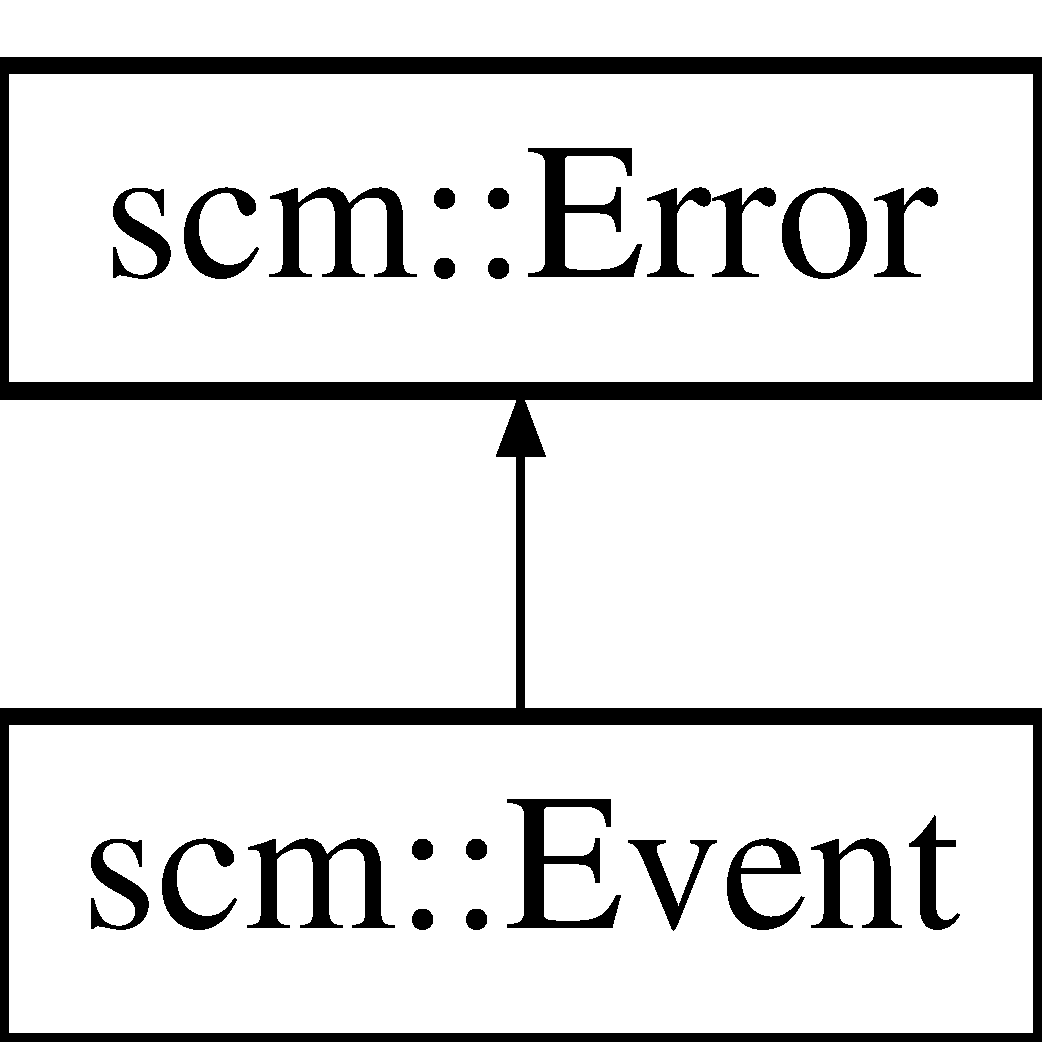
\includegraphics[height=2cm]{classscm_1_1_error}
\end{center}
\end{figure}
\subsection*{Public Member Functions}
\begin{DoxyCompactItemize}
\item 
\hyperlink{classscm_1_1_error_a9c6aa255ce180155a748f304f83830d3}{Error} (\hyperlink{namespacescm_a13a6ecf77ceb7b5b3a38e0fada54aa99}{ErrString} es)
\item 
virtual bool \hyperlink{classscm_1_1_error_a2660b73f9671be3f286bed9d622a926a}{Ok} ()=0
\item 
\hyperlink{namespacescm_a13a6ecf77ceb7b5b3a38e0fada54aa99}{ErrString} \hyperlink{classscm_1_1_error_a8fa002269b2ea7b0af4581951a7908f0}{Err} ()
\item 
void \hyperlink{classscm_1_1_error_aa4309b2556e84bd9bc6c7871f3be2f7a}{Err} (\hyperlink{namespacescm_a13a6ecf77ceb7b5b3a38e0fada54aa99}{ErrString} es)
\item 
void \hyperlink{classscm_1_1_error_a4dc4a630569665a615a0bfb321b65238}{ReportErr} ()
\item 
void \hyperlink{classscm_1_1_error_ace08c93643469a92cb3ca1e0fb1ca583}{SetReportErr} (\hyperlink{namespacescm_a13a6ecf77ceb7b5b3a38e0fada54aa99}{ErrString} es)
\item 
void \hyperlink{classscm_1_1_error_a3d3598611ee2955f3144ec2602b69677}{ClassName} (std::string cn)
\end{DoxyCompactItemize}


\subsection{Detailed Description}


Definition at line 9 of file error.h.



\subsection{Constructor \& Destructor Documentation}
\hypertarget{classscm_1_1_error_a9c6aa255ce180155a748f304f83830d3}{
\index{scm::Error@{scm::Error}!Error@{Error}}
\index{Error@{Error}!scm::Error@{scm::Error}}
\subsubsection[{Error}]{\setlength{\rightskip}{0pt plus 5cm}scm::Error::Error ({\bf ErrString} {\em es})}}
\label{classscm_1_1_error_a9c6aa255ce180155a748f304f83830d3}


Definition at line 11 of file error.cc.



\subsection{Member Function Documentation}
\hypertarget{classscm_1_1_error_a3d3598611ee2955f3144ec2602b69677}{
\index{scm::Error@{scm::Error}!ClassName@{ClassName}}
\index{ClassName@{ClassName}!scm::Error@{scm::Error}}
\subsubsection[{ClassName}]{\setlength{\rightskip}{0pt plus 5cm}void scm::Error::ClassName (std::string {\em cn})\hspace{0.3cm}{\ttfamily  \mbox{[}inline\mbox{]}}}}
\label{classscm_1_1_error_a3d3598611ee2955f3144ec2602b69677}


Definition at line 25 of file error.h.

\hypertarget{classscm_1_1_error_aa4309b2556e84bd9bc6c7871f3be2f7a}{
\index{scm::Error@{scm::Error}!Err@{Err}}
\index{Err@{Err}!scm::Error@{scm::Error}}
\subsubsection[{Err}]{\setlength{\rightskip}{0pt plus 5cm}void scm::Error::Err ({\bf scm::ErrString} {\em es})}}
\label{classscm_1_1_error_aa4309b2556e84bd9bc6c7871f3be2f7a}


Definition at line 21 of file error.cc.

\hypertarget{classscm_1_1_error_a8fa002269b2ea7b0af4581951a7908f0}{
\index{scm::Error@{scm::Error}!Err@{Err}}
\index{Err@{Err}!scm::Error@{scm::Error}}
\subsubsection[{Err}]{\setlength{\rightskip}{0pt plus 5cm}{\bf ErrString} scm::Error::Err ()}}
\label{classscm_1_1_error_a8fa002269b2ea7b0af4581951a7908f0}


Definition at line 15 of file error.cc.

\hypertarget{classscm_1_1_error_a2660b73f9671be3f286bed9d622a926a}{
\index{scm::Error@{scm::Error}!Ok@{Ok}}
\index{Ok@{Ok}!scm::Error@{scm::Error}}
\subsubsection[{Ok}]{\setlength{\rightskip}{0pt plus 5cm}virtual bool scm::Error::Ok ()\hspace{0.3cm}{\ttfamily  \mbox{[}pure virtual\mbox{]}}}}
\label{classscm_1_1_error_a2660b73f9671be3f286bed9d622a926a}


Implemented in \hyperlink{classscm_1_1_event_a95400a0d0218dfb664c028d1130a5d14}{scm::Event}.

\hypertarget{classscm_1_1_error_a4dc4a630569665a615a0bfb321b65238}{
\index{scm::Error@{scm::Error}!ReportErr@{ReportErr}}
\index{ReportErr@{ReportErr}!scm::Error@{scm::Error}}
\subsubsection[{ReportErr}]{\setlength{\rightskip}{0pt plus 5cm}void scm::Error::ReportErr ()}}
\label{classscm_1_1_error_a4dc4a630569665a615a0bfb321b65238}


Definition at line 29 of file error.cc.

\hypertarget{classscm_1_1_error_ace08c93643469a92cb3ca1e0fb1ca583}{
\index{scm::Error@{scm::Error}!SetReportErr@{SetReportErr}}
\index{SetReportErr@{SetReportErr}!scm::Error@{scm::Error}}
\subsubsection[{SetReportErr}]{\setlength{\rightskip}{0pt plus 5cm}void scm::Error::SetReportErr ({\bf ErrString} {\em es})}}
\label{classscm_1_1_error_ace08c93643469a92cb3ca1e0fb1ca583}


Definition at line 33 of file error.cc.



The documentation for this class was generated from the following files:\begin{DoxyCompactItemize}
\item 
/home/derek/dev/crml/crml/src/sys/\hyperlink{error_8h}{error.h}\item 
/home/derek/dev/crml/crml/src/sys/\hyperlink{error_8cc}{error.cc}\end{DoxyCompactItemize}

\hypertarget{classscm_1_1_event}{
\section{scm::Event Class Reference}
\label{classscm_1_1_event}\index{scm::Event@{scm::Event}}
}


{\ttfamily \#include $<$event.h$>$}

Inheritance diagram for scm::Event:\begin{figure}[H]
\begin{center}
\leavevmode
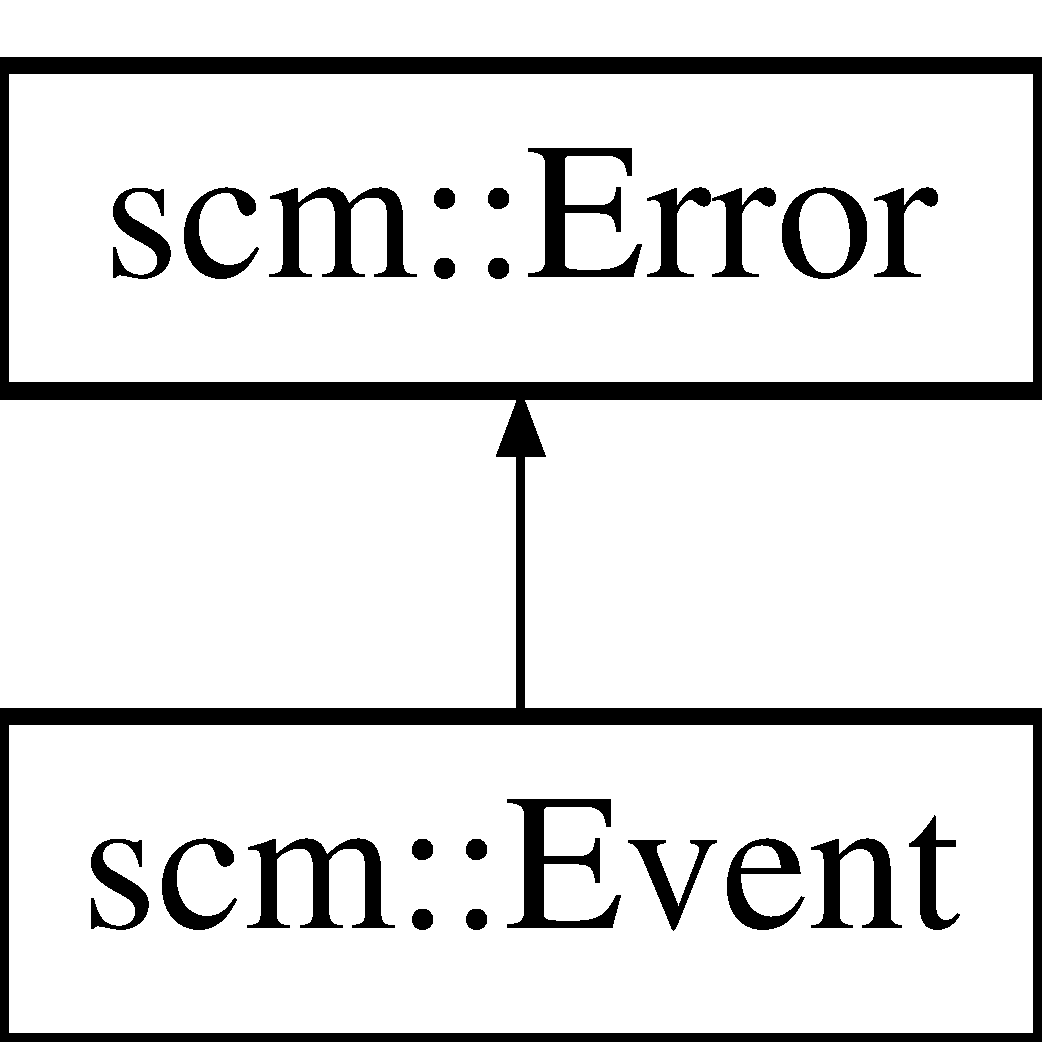
\includegraphics[height=2cm]{classscm_1_1_event}
\end{center}
\end{figure}
\subsection*{Public Member Functions}
\begin{DoxyCompactItemize}
\item 
\hyperlink{classscm_1_1_event_ae0b0fbe856c9fbce52b50e08860946e8}{Event} ()
\item 
\hyperlink{classscm_1_1_event_a4f22bf217daf2b5e3670e987579fb152}{$\sim$Event} ()
\item 
void \hyperlink{classscm_1_1_event_a2dfdf12d5b7918b2102e7ce1c4142ed3}{Init} ()
\item 
void \hyperlink{classscm_1_1_event_a1e1aa9fbe9b5e7e7c9b0ff8f0ba74cd2}{PushEvent} (\hyperlink{struct___n_p_pepper_event}{NPPepperEvent} $\ast$evt)
\item 
bool \hyperlink{classscm_1_1_event_ae736ee83efd335726cad841b6082e491}{Empty} ()
\item 
void \hyperlink{classscm_1_1_event_aba1e9492e1d03bd67afb9c8943e89fe9}{Drain} ()
\item 
\hyperlink{struct___n_p_pepper_event}{NPPepperEvent} $\ast$ \hyperlink{classscm_1_1_event_aaa7905956b3d789fa16cc7a73490dc5e}{PopEvent} ()
\item 
virtual bool \hyperlink{classscm_1_1_event_a95400a0d0218dfb664c028d1130a5d14}{Ok} ()
\end{DoxyCompactItemize}


\subsection{Detailed Description}


Definition at line 19 of file event.h.



\subsection{Constructor \& Destructor Documentation}
\hypertarget{classscm_1_1_event_ae0b0fbe856c9fbce52b50e08860946e8}{
\index{scm::Event@{scm::Event}!Event@{Event}}
\index{Event@{Event}!scm::Event@{scm::Event}}
\subsubsection[{Event}]{\setlength{\rightskip}{0pt plus 5cm}scm::Event::Event ()\hspace{0.3cm}{\ttfamily  \mbox{[}inline, explicit\mbox{]}}}}
\label{classscm_1_1_event_ae0b0fbe856c9fbce52b50e08860946e8}


Definition at line 21 of file event.h.

\hypertarget{classscm_1_1_event_a4f22bf217daf2b5e3670e987579fb152}{
\index{scm::Event@{scm::Event}!$\sim$Event@{$\sim$Event}}
\index{$\sim$Event@{$\sim$Event}!scm::Event@{scm::Event}}
\subsubsection[{$\sim$Event}]{\setlength{\rightskip}{0pt plus 5cm}scm::Event::$\sim$Event ()}}
\label{classscm_1_1_event_a4f22bf217daf2b5e3670e987579fb152}


Definition at line 17 of file event.cc.



\subsection{Member Function Documentation}
\hypertarget{classscm_1_1_event_aba1e9492e1d03bd67afb9c8943e89fe9}{
\index{scm::Event@{scm::Event}!Drain@{Drain}}
\index{Drain@{Drain}!scm::Event@{scm::Event}}
\subsubsection[{Drain}]{\setlength{\rightskip}{0pt plus 5cm}void scm::Event::Drain ()}}
\label{classscm_1_1_event_aba1e9492e1d03bd67afb9c8943e89fe9}


Definition at line 59 of file event.cc.

\hypertarget{classscm_1_1_event_ae736ee83efd335726cad841b6082e491}{
\index{scm::Event@{scm::Event}!Empty@{Empty}}
\index{Empty@{Empty}!scm::Event@{scm::Event}}
\subsubsection[{Empty}]{\setlength{\rightskip}{0pt plus 5cm}bool scm::Event::Empty ()}}
\label{classscm_1_1_event_ae736ee83efd335726cad841b6082e491}


Definition at line 26 of file event.cc.

\hypertarget{classscm_1_1_event_a2dfdf12d5b7918b2102e7ce1c4142ed3}{
\index{scm::Event@{scm::Event}!Init@{Init}}
\index{Init@{Init}!scm::Event@{scm::Event}}
\subsubsection[{Init}]{\setlength{\rightskip}{0pt plus 5cm}void scm::Event::Init ()}}
\label{classscm_1_1_event_a2dfdf12d5b7918b2102e7ce1c4142ed3}


Definition at line 21 of file event.cc.

\hypertarget{classscm_1_1_event_a95400a0d0218dfb664c028d1130a5d14}{
\index{scm::Event@{scm::Event}!Ok@{Ok}}
\index{Ok@{Ok}!scm::Event@{scm::Event}}
\subsubsection[{Ok}]{\setlength{\rightskip}{0pt plus 5cm}bool scm::Event::Ok ()\hspace{0.3cm}{\ttfamily  \mbox{[}virtual\mbox{]}}}}
\label{classscm_1_1_event_a95400a0d0218dfb664c028d1130a5d14}


Implements \hyperlink{classscm_1_1_error_a2660b73f9671be3f286bed9d622a926a}{scm::Error}.



Definition at line 13 of file event.cc.

\hypertarget{classscm_1_1_event_aaa7905956b3d789fa16cc7a73490dc5e}{
\index{scm::Event@{scm::Event}!PopEvent@{PopEvent}}
\index{PopEvent@{PopEvent}!scm::Event@{scm::Event}}
\subsubsection[{PopEvent}]{\setlength{\rightskip}{0pt plus 5cm}{\bf NPPepperEvent} $\ast$ scm::Event::PopEvent ()}}
\label{classscm_1_1_event_aaa7905956b3d789fa16cc7a73490dc5e}


Definition at line 50 of file event.cc.

\hypertarget{classscm_1_1_event_a1e1aa9fbe9b5e7e7c9b0ff8f0ba74cd2}{
\index{scm::Event@{scm::Event}!PushEvent@{PushEvent}}
\index{PushEvent@{PushEvent}!scm::Event@{scm::Event}}
\subsubsection[{PushEvent}]{\setlength{\rightskip}{0pt plus 5cm}void scm::Event::PushEvent ({\bf NPPepperEvent} $\ast$ {\em evt})}}
\label{classscm_1_1_event_a1e1aa9fbe9b5e7e7c9b0ff8f0ba74cd2}


Definition at line 65 of file event.cc.



The documentation for this class was generated from the following files:\begin{DoxyCompactItemize}
\item 
/home/derek/dev/cell-\/grid-\/game/nacl/crml/crml/evt/\hyperlink{event_8h}{event.h}\item 
/home/derek/dev/cell-\/grid-\/game/nacl/crml/crml/evt/\hyperlink{event_8cc}{event.cc}\end{DoxyCompactItemize}

\hypertarget{class_event_handler}{
\section{EventHandler Class Reference}
\label{class_event_handler}\index{EventHandler@{EventHandler}}
}


{\ttfamily \#include $<$event\_\-handler.h$>$}

\subsection*{Public Member Functions}
\begin{DoxyCompactItemize}
\item 
\hyperlink{class_event_handler_a6b7f9af8b5c3c4128047d35467ca0da0}{EventHandler} (\hyperlink{struct___n_p_p}{NPP} npp)
\item 
\hyperlink{class_event_handler_a3decb8cd88ba8af2b9b0b0f0f2fcd722}{$\sim$EventHandler} ()
\item 
bool \hyperlink{class_event_handler_a18771c6be120edf9d912a4003066b8b3}{addText} (const char $\ast$cstr)
\item 
int \hyperlink{class_event_handler_a2fcafd6f528017d8a814f9c384e2e057}{handle} (void $\ast$event)
\item 
bool \hyperlink{class_event_handler_a2f334e3eb39be72751e342619489e695}{is\_\-text\_\-box\_\-set} ()
\item 
bool \hyperlink{class_event_handler_aa09c0b995aa6c774d4a33be13be0cbf2}{set\_\-text\_\-box} (NPObject $\ast$text\_\-box\_\-object)
\item 
void \hyperlink{class_event_handler_a67d149352861c0a8fe603a14585d1003}{Init} (\hyperlink{classscm_1_1_event}{scm::Event} $\ast$)
\end{DoxyCompactItemize}


\subsection{Detailed Description}


Definition at line 34 of file event\_\-handler.h.



\subsection{Constructor \& Destructor Documentation}
\hypertarget{class_event_handler_a6b7f9af8b5c3c4128047d35467ca0da0}{
\index{EventHandler@{EventHandler}!EventHandler@{EventHandler}}
\index{EventHandler@{EventHandler}!EventHandler@{EventHandler}}
\subsubsection[{EventHandler}]{\setlength{\rightskip}{0pt plus 5cm}EventHandler::EventHandler ({\bf NPP} {\em npp})\hspace{0.3cm}{\ttfamily  \mbox{[}explicit\mbox{]}}}}
\label{class_event_handler_a6b7f9af8b5c3c4128047d35467ca0da0}


Definition at line 57 of file event\_\-handler.cc.

\hypertarget{class_event_handler_a3decb8cd88ba8af2b9b0b0f0f2fcd722}{
\index{EventHandler@{EventHandler}!$\sim$EventHandler@{$\sim$EventHandler}}
\index{$\sim$EventHandler@{$\sim$EventHandler}!EventHandler@{EventHandler}}
\subsubsection[{$\sim$EventHandler}]{\setlength{\rightskip}{0pt plus 5cm}EventHandler::$\sim$EventHandler ()}}
\label{class_event_handler_a3decb8cd88ba8af2b9b0b0f0f2fcd722}


Definition at line 62 of file event\_\-handler.cc.



\subsection{Member Function Documentation}
\hypertarget{class_event_handler_a18771c6be120edf9d912a4003066b8b3}{
\index{EventHandler@{EventHandler}!addText@{addText}}
\index{addText@{addText}!EventHandler@{EventHandler}}
\subsubsection[{addText}]{\setlength{\rightskip}{0pt plus 5cm}bool EventHandler::addText (const char $\ast$ {\em cstr})}}
\label{class_event_handler_a18771c6be120edf9d912a4003066b8b3}


Definition at line 71 of file event\_\-handler.cc.

\hypertarget{class_event_handler_a2fcafd6f528017d8a814f9c384e2e057}{
\index{EventHandler@{EventHandler}!handle@{handle}}
\index{handle@{handle}!EventHandler@{EventHandler}}
\subsubsection[{handle}]{\setlength{\rightskip}{0pt plus 5cm}int EventHandler::handle (void $\ast$ {\em event})}}
\label{class_event_handler_a2fcafd6f528017d8a814f9c384e2e057}


Definition at line 121 of file event\_\-handler.cc.

\hypertarget{class_event_handler_a67d149352861c0a8fe603a14585d1003}{
\index{EventHandler@{EventHandler}!Init@{Init}}
\index{Init@{Init}!EventHandler@{EventHandler}}
\subsubsection[{Init}]{\setlength{\rightskip}{0pt plus 5cm}void EventHandler::Init ({\bf scm::Event} $\ast$ {\em sys})}}
\label{class_event_handler_a67d149352861c0a8fe603a14585d1003}


Definition at line 65 of file event\_\-handler.cc.

\hypertarget{class_event_handler_a2f334e3eb39be72751e342619489e695}{
\index{EventHandler@{EventHandler}!is\_\-text\_\-box\_\-set@{is\_\-text\_\-box\_\-set}}
\index{is\_\-text\_\-box\_\-set@{is\_\-text\_\-box\_\-set}!EventHandler@{EventHandler}}
\subsubsection[{is\_\-text\_\-box\_\-set}]{\setlength{\rightskip}{0pt plus 5cm}bool EventHandler::is\_\-text\_\-box\_\-set ()}}
\label{class_event_handler_a2f334e3eb39be72751e342619489e695}


Definition at line 187 of file event\_\-handler.cc.

\hypertarget{class_event_handler_aa09c0b995aa6c774d4a33be13be0cbf2}{
\index{EventHandler@{EventHandler}!set\_\-text\_\-box@{set\_\-text\_\-box}}
\index{set\_\-text\_\-box@{set\_\-text\_\-box}!EventHandler@{EventHandler}}
\subsubsection[{set\_\-text\_\-box}]{\setlength{\rightskip}{0pt plus 5cm}bool EventHandler::set\_\-text\_\-box (NPObject $\ast$ {\em text\_\-box\_\-object})}}
\label{class_event_handler_aa09c0b995aa6c774d4a33be13be0cbf2}


Definition at line 193 of file event\_\-handler.cc.



The documentation for this class was generated from the following files:\begin{DoxyCompactItemize}
\item 
/home/derek/dev/cell-\/grid-\/game/nacl/crml/crml/evt/\hyperlink{event__handler_8h}{event\_\-handler.h}\item 
/home/derek/dev/cell-\/grid-\/game/nacl/crml/crml/evt/\hyperlink{event__handler_8cc}{event\_\-handler.cc}\end{DoxyCompactItemize}

\hypertarget{class_hello_world_instance}{
\section{HelloWorldInstance Class Reference}
\label{class_hello_world_instance}\index{HelloWorldInstance@{HelloWorldInstance}}
}
\subsection*{Public Member Functions}
\begin{DoxyCompactItemize}
\item 
\hyperlink{class_hello_world_instance_add03eac81a09900135582a464bfcd8f8}{HelloWorldInstance} (PP\_\-Instance instance)
\item 
virtual \hyperlink{class_hello_world_instance_ab82a0f1aa35b3f8fbc2e107af026bfc5}{$\sim$HelloWorldInstance} ()
\item 
virtual pp::Var \hyperlink{class_hello_world_instance_ac489a6775aead72dc1b17d22d1eb6688}{GetInstanceObject} ()
\end{DoxyCompactItemize}


\subsection{Detailed Description}


Definition at line 102 of file hello\_\-world.cc.



\subsection{Constructor \& Destructor Documentation}
\hypertarget{class_hello_world_instance_add03eac81a09900135582a464bfcd8f8}{
\index{HelloWorldInstance@{HelloWorldInstance}!HelloWorldInstance@{HelloWorldInstance}}
\index{HelloWorldInstance@{HelloWorldInstance}!HelloWorldInstance@{HelloWorldInstance}}
\subsubsection[{HelloWorldInstance}]{\setlength{\rightskip}{0pt plus 5cm}HelloWorldInstance::HelloWorldInstance (PP\_\-Instance {\em instance})\hspace{0.3cm}{\ttfamily  \mbox{[}inline\mbox{]}}}}
\label{class_hello_world_instance_add03eac81a09900135582a464bfcd8f8}


Definition at line 104 of file hello\_\-world.cc.

\hypertarget{class_hello_world_instance_ab82a0f1aa35b3f8fbc2e107af026bfc5}{
\index{HelloWorldInstance@{HelloWorldInstance}!$\sim$HelloWorldInstance@{$\sim$HelloWorldInstance}}
\index{$\sim$HelloWorldInstance@{$\sim$HelloWorldInstance}!HelloWorldInstance@{HelloWorldInstance}}
\subsubsection[{$\sim$HelloWorldInstance}]{\setlength{\rightskip}{0pt plus 5cm}virtual HelloWorldInstance::$\sim$HelloWorldInstance ()\hspace{0.3cm}{\ttfamily  \mbox{[}inline, virtual\mbox{]}}}}
\label{class_hello_world_instance_ab82a0f1aa35b3f8fbc2e107af026bfc5}


Definition at line 105 of file hello\_\-world.cc.



\subsection{Member Function Documentation}
\hypertarget{class_hello_world_instance_ac489a6775aead72dc1b17d22d1eb6688}{
\index{HelloWorldInstance@{HelloWorldInstance}!GetInstanceObject@{GetInstanceObject}}
\index{GetInstanceObject@{GetInstanceObject}!HelloWorldInstance@{HelloWorldInstance}}
\subsubsection[{GetInstanceObject}]{\setlength{\rightskip}{0pt plus 5cm}virtual pp::Var HelloWorldInstance::GetInstanceObject ()\hspace{0.3cm}{\ttfamily  \mbox{[}inline, virtual\mbox{]}}}}
\label{class_hello_world_instance_ac489a6775aead72dc1b17d22d1eb6688}


Definition at line 108 of file hello\_\-world.cc.



The documentation for this class was generated from the following file:\begin{DoxyCompactItemize}
\item 
/home/derek/dev/crml/crml/test/hello\_\-world/\hyperlink{hello__world_8cc}{hello\_\-world.cc}\end{DoxyCompactItemize}

\hypertarget{class_hello_world_module}{
\section{HelloWorldModule Class Reference}
\label{class_hello_world_module}\index{HelloWorldModule@{HelloWorldModule}}
}
\subsection*{Public Member Functions}
\begin{DoxyCompactItemize}
\item 
\hyperlink{class_hello_world_module_a51bebf2cbff1d8914b988101781bd01d}{HelloWorldModule} ()
\item 
virtual \hyperlink{class_hello_world_module_a2458f9ee6a26568e54c6bd3a0323abcf}{$\sim$HelloWorldModule} ()
\item 
virtual pp::Instance $\ast$ \hyperlink{class_hello_world_module_a6ee0eeeb3ed2f95b819adfd4df33c47f}{CreateInstance} (PP\_\-Instance instance)
\end{DoxyCompactItemize}


\subsection{Detailed Description}


Definition at line 117 of file hello\_\-world.cc.



\subsection{Constructor \& Destructor Documentation}
\hypertarget{class_hello_world_module_a51bebf2cbff1d8914b988101781bd01d}{
\index{HelloWorldModule@{HelloWorldModule}!HelloWorldModule@{HelloWorldModule}}
\index{HelloWorldModule@{HelloWorldModule}!HelloWorldModule@{HelloWorldModule}}
\subsubsection[{HelloWorldModule}]{\setlength{\rightskip}{0pt plus 5cm}HelloWorldModule::HelloWorldModule ()\hspace{0.3cm}{\ttfamily  \mbox{[}inline\mbox{]}}}}
\label{class_hello_world_module_a51bebf2cbff1d8914b988101781bd01d}


Definition at line 119 of file hello\_\-world.cc.

\hypertarget{class_hello_world_module_a2458f9ee6a26568e54c6bd3a0323abcf}{
\index{HelloWorldModule@{HelloWorldModule}!$\sim$HelloWorldModule@{$\sim$HelloWorldModule}}
\index{$\sim$HelloWorldModule@{$\sim$HelloWorldModule}!HelloWorldModule@{HelloWorldModule}}
\subsubsection[{$\sim$HelloWorldModule}]{\setlength{\rightskip}{0pt plus 5cm}virtual HelloWorldModule::$\sim$HelloWorldModule ()\hspace{0.3cm}{\ttfamily  \mbox{[}inline, virtual\mbox{]}}}}
\label{class_hello_world_module_a2458f9ee6a26568e54c6bd3a0323abcf}


Definition at line 120 of file hello\_\-world.cc.



\subsection{Member Function Documentation}
\hypertarget{class_hello_world_module_a6ee0eeeb3ed2f95b819adfd4df33c47f}{
\index{HelloWorldModule@{HelloWorldModule}!CreateInstance@{CreateInstance}}
\index{CreateInstance@{CreateInstance}!HelloWorldModule@{HelloWorldModule}}
\subsubsection[{CreateInstance}]{\setlength{\rightskip}{0pt plus 5cm}virtual pp::Instance$\ast$ HelloWorldModule::CreateInstance (PP\_\-Instance {\em instance})\hspace{0.3cm}{\ttfamily  \mbox{[}inline, virtual\mbox{]}}}}
\label{class_hello_world_module_a6ee0eeeb3ed2f95b819adfd4df33c47f}


Definition at line 123 of file hello\_\-world.cc.



The documentation for this class was generated from the following file:\begin{DoxyCompactItemize}
\item 
/home/derek/dev/cell-\/grid-\/game/nacl/crml/crml/test/hello\_\-world/\hyperlink{hello__world_8cc}{hello\_\-world.cc}\end{DoxyCompactItemize}

\hypertarget{class_hello_world_scriptable_object}{
\section{HelloWorldScriptableObject Class Reference}
\label{class_hello_world_scriptable_object}\index{HelloWorldScriptableObject@{HelloWorldScriptableObject}}
}
\subsection*{Public Member Functions}
\begin{DoxyCompactItemize}
\item 
virtual bool \hyperlink{class_hello_world_scriptable_object_a0af23165c74483e47f97877cbb51e79a}{HasMethod} (const pp::Var \&method, pp::Var $\ast$exception)
\item 
virtual pp::Var \hyperlink{class_hello_world_scriptable_object_a217b4b958a4bfb250dd8ac588ab794ad}{Call} (const pp::Var \&method, const std::vector$<$ pp::Var $>$ \&args, pp::Var $\ast$exception)
\end{DoxyCompactItemize}


\subsection{Detailed Description}


Definition at line 53 of file hello\_\-world.cc.



\subsection{Member Function Documentation}
\hypertarget{class_hello_world_scriptable_object_a217b4b958a4bfb250dd8ac588ab794ad}{
\index{HelloWorldScriptableObject@{HelloWorldScriptableObject}!Call@{Call}}
\index{Call@{Call}!HelloWorldScriptableObject@{HelloWorldScriptableObject}}
\subsubsection[{Call}]{\setlength{\rightskip}{0pt plus 5cm}pp::Var HelloWorldScriptableObject::Call (const pp::Var \& {\em method}, \/  const std::vector$<$ pp::Var $>$ \& {\em args}, \/  pp::Var $\ast$ {\em exception})\hspace{0.3cm}{\ttfamily  \mbox{[}virtual\mbox{]}}}}
\label{class_hello_world_scriptable_object_a217b4b958a4bfb250dd8ac588ab794ad}


Definition at line 77 of file hello\_\-world.cc.

\hypertarget{class_hello_world_scriptable_object_a0af23165c74483e47f97877cbb51e79a}{
\index{HelloWorldScriptableObject@{HelloWorldScriptableObject}!HasMethod@{HasMethod}}
\index{HasMethod@{HasMethod}!HelloWorldScriptableObject@{HelloWorldScriptableObject}}
\subsubsection[{HasMethod}]{\setlength{\rightskip}{0pt plus 5cm}bool HelloWorldScriptableObject::HasMethod (const pp::Var \& {\em method}, \/  pp::Var $\ast$ {\em exception})\hspace{0.3cm}{\ttfamily  \mbox{[}virtual\mbox{]}}}}
\label{class_hello_world_scriptable_object_a0af23165c74483e47f97877cbb51e79a}


Definition at line 66 of file hello\_\-world.cc.



The documentation for this class was generated from the following file:\begin{DoxyCompactItemize}
\item 
/home/derek/dev/cell-\/grid-\/game/nacl/crml/crml/test/hello\_\-world/\hyperlink{hello__world_8cc}{hello\_\-world.cc}\end{DoxyCompactItemize}

\hypertarget{classscm_1_1_hex_store}{
\section{scm::HexStore Class Reference}
\label{classscm_1_1_hex_store}\index{scm::HexStore@{scm::HexStore}}
}


{\ttfamily \#include $<$hex\_\-store.h$>$}

\subsection*{Public Member Functions}
\begin{DoxyCompactItemize}
\item 
\hyperlink{classscm_1_1_hex_store_ae3ea77bf45ef55916e02aba5f5d280f5}{HexStore} ()
\item 
\hyperlink{classscm_1_1_hex_store_ac418965e7e9ee7569bb03b7230bad1bd}{$\sim$HexStore} ()
\item 
bool \hyperlink{classscm_1_1_hex_store_ae8d894818fe0859462b63f2e34d08a33}{Ok} ()
\item 
int \hyperlink{classscm_1_1_hex_store_a85cbfdc7f9a41355db174d3b96382d79}{Err} ()
\item 
void \hyperlink{classscm_1_1_hex_store_ac98d4c0f37c642e6b45262ec1db62d80}{ReportErr} ()
\item 
void \hyperlink{classscm_1_1_hex_store_aa1792118dbb32383976d6906c69c9e71}{Store} (std::string, std::string)
\item 
int \hyperlink{classscm_1_1_hex_store_a277a7c2220511ad3c0e447802589def1}{ValLength} (std::string)
\item 
bool \hyperlink{classscm_1_1_hex_store_a2c7a1fc73741e0b3613516388b562475}{EmptyVal} (std::string)
\item 
void \hyperlink{classscm_1_1_hex_store_ac086449d331c2e0dd6eaf11a003ffe99}{Append} (std::string, std::string)
\item 
std::string \hyperlink{classscm_1_1_hex_store_acdc20757093a52e3f7748dea41d185b2}{GetValue} (std::string)
\item 
const char $\ast$ \hyperlink{classscm_1_1_hex_store_a5e12c88428e17be9bb8f6c08ab107e57}{ByteArray} (std::string)
\end{DoxyCompactItemize}


\subsection{Detailed Description}


Definition at line 19 of file hex\_\-store.h.



\subsection{Constructor \& Destructor Documentation}
\hypertarget{classscm_1_1_hex_store_ae3ea77bf45ef55916e02aba5f5d280f5}{
\index{scm::HexStore@{scm::HexStore}!HexStore@{HexStore}}
\index{HexStore@{HexStore}!scm::HexStore@{scm::HexStore}}
\subsubsection[{HexStore}]{\setlength{\rightskip}{0pt plus 5cm}scm::HexStore::HexStore ()}}
\label{classscm_1_1_hex_store_ae3ea77bf45ef55916e02aba5f5d280f5}


Definition at line 11 of file hex\_\-store.cc.

\hypertarget{classscm_1_1_hex_store_ac418965e7e9ee7569bb03b7230bad1bd}{
\index{scm::HexStore@{scm::HexStore}!$\sim$HexStore@{$\sim$HexStore}}
\index{$\sim$HexStore@{$\sim$HexStore}!scm::HexStore@{scm::HexStore}}
\subsubsection[{$\sim$HexStore}]{\setlength{\rightskip}{0pt plus 5cm}scm::HexStore::$\sim$HexStore ()}}
\label{classscm_1_1_hex_store_ac418965e7e9ee7569bb03b7230bad1bd}


Definition at line 12 of file hex\_\-store.cc.



\subsection{Member Function Documentation}
\hypertarget{classscm_1_1_hex_store_ac086449d331c2e0dd6eaf11a003ffe99}{
\index{scm::HexStore@{scm::HexStore}!Append@{Append}}
\index{Append@{Append}!scm::HexStore@{scm::HexStore}}
\subsubsection[{Append}]{\setlength{\rightskip}{0pt plus 5cm}void scm::HexStore::Append (std::string {\em key}, \/  std::string {\em val})}}
\label{classscm_1_1_hex_store_ac086449d331c2e0dd6eaf11a003ffe99}


Definition at line 67 of file hex\_\-store.cc.

\hypertarget{classscm_1_1_hex_store_a5e12c88428e17be9bb8f6c08ab107e57}{
\index{scm::HexStore@{scm::HexStore}!ByteArray@{ByteArray}}
\index{ByteArray@{ByteArray}!scm::HexStore@{scm::HexStore}}
\subsubsection[{ByteArray}]{\setlength{\rightskip}{0pt plus 5cm}const char $\ast$ scm::HexStore::ByteArray (std::string {\em key})}}
\label{classscm_1_1_hex_store_a5e12c88428e17be9bb8f6c08ab107e57}


Definition at line 79 of file hex\_\-store.cc.

\hypertarget{classscm_1_1_hex_store_a2c7a1fc73741e0b3613516388b562475}{
\index{scm::HexStore@{scm::HexStore}!EmptyVal@{EmptyVal}}
\index{EmptyVal@{EmptyVal}!scm::HexStore@{scm::HexStore}}
\subsubsection[{EmptyVal}]{\setlength{\rightskip}{0pt plus 5cm}bool scm::HexStore::EmptyVal (std::string {\em key})}}
\label{classscm_1_1_hex_store_a2c7a1fc73741e0b3613516388b562475}


Definition at line 45 of file hex\_\-store.cc.

\hypertarget{classscm_1_1_hex_store_a85cbfdc7f9a41355db174d3b96382d79}{
\index{scm::HexStore@{scm::HexStore}!Err@{Err}}
\index{Err@{Err}!scm::HexStore@{scm::HexStore}}
\subsubsection[{Err}]{\setlength{\rightskip}{0pt plus 5cm}int scm::HexStore::Err ()}}
\label{classscm_1_1_hex_store_a85cbfdc7f9a41355db174d3b96382d79}


Definition at line 15 of file hex\_\-store.cc.

\hypertarget{classscm_1_1_hex_store_acdc20757093a52e3f7748dea41d185b2}{
\index{scm::HexStore@{scm::HexStore}!GetValue@{GetValue}}
\index{GetValue@{GetValue}!scm::HexStore@{scm::HexStore}}
\subsubsection[{GetValue}]{\setlength{\rightskip}{0pt plus 5cm}std::string scm::HexStore::GetValue (std::string {\em key})}}
\label{classscm_1_1_hex_store_acdc20757093a52e3f7748dea41d185b2}


Definition at line 58 of file hex\_\-store.cc.

\hypertarget{classscm_1_1_hex_store_ae8d894818fe0859462b63f2e34d08a33}{
\index{scm::HexStore@{scm::HexStore}!Ok@{Ok}}
\index{Ok@{Ok}!scm::HexStore@{scm::HexStore}}
\subsubsection[{Ok}]{\setlength{\rightskip}{0pt plus 5cm}bool scm::HexStore::Ok ()}}
\label{classscm_1_1_hex_store_ae8d894818fe0859462b63f2e34d08a33}


Definition at line 19 of file hex\_\-store.cc.

\hypertarget{classscm_1_1_hex_store_ac98d4c0f37c642e6b45262ec1db62d80}{
\index{scm::HexStore@{scm::HexStore}!ReportErr@{ReportErr}}
\index{ReportErr@{ReportErr}!scm::HexStore@{scm::HexStore}}
\subsubsection[{ReportErr}]{\setlength{\rightskip}{0pt plus 5cm}void scm::HexStore::ReportErr ()}}
\label{classscm_1_1_hex_store_ac98d4c0f37c642e6b45262ec1db62d80}


Definition at line 23 of file hex\_\-store.cc.

\hypertarget{classscm_1_1_hex_store_aa1792118dbb32383976d6906c69c9e71}{
\index{scm::HexStore@{scm::HexStore}!Store@{Store}}
\index{Store@{Store}!scm::HexStore@{scm::HexStore}}
\subsubsection[{Store}]{\setlength{\rightskip}{0pt plus 5cm}void scm::HexStore::Store (std::string {\em key}, \/  std::string {\em val})}}
\label{classscm_1_1_hex_store_aa1792118dbb32383976d6906c69c9e71}


Definition at line 40 of file hex\_\-store.cc.

\hypertarget{classscm_1_1_hex_store_a277a7c2220511ad3c0e447802589def1}{
\index{scm::HexStore@{scm::HexStore}!ValLength@{ValLength}}
\index{ValLength@{ValLength}!scm::HexStore@{scm::HexStore}}
\subsubsection[{ValLength}]{\setlength{\rightskip}{0pt plus 5cm}int scm::HexStore::ValLength (std::string {\em key})}}
\label{classscm_1_1_hex_store_a277a7c2220511ad3c0e447802589def1}


Definition at line 49 of file hex\_\-store.cc.



The documentation for this class was generated from the following files:\begin{DoxyCompactItemize}
\item 
/home/derek/dev/cell-\/grid-\/game/nacl/crml/crml/sys/\hyperlink{hex__store_8h}{hex\_\-store.h}\item 
/home/derek/dev/cell-\/grid-\/game/nacl/crml/crml/sys/\hyperlink{hex__store_8cc}{hex\_\-store.cc}\end{DoxyCompactItemize}

\hypertarget{struct_m_d5_digest__struct}{
\section{MD5Digest\_\-struct Struct Reference}
\label{struct_m_d5_digest__struct}\index{MD5Digest\_\-struct@{MD5Digest\_\-struct}}
}


{\ttfamily \#include $<$md5.h$>$}

\subsection*{Public Attributes}
\begin{DoxyCompactItemize}
\item 
unsigned char \hyperlink{struct_m_d5_digest__struct_a47ba426c0b835e8947717e860464b255}{a} \mbox{[}16\mbox{]}
\end{DoxyCompactItemize}


\subsection{Detailed Description}


Definition at line 34 of file md5.h.



\subsection{Member Data Documentation}
\hypertarget{struct_m_d5_digest__struct_a47ba426c0b835e8947717e860464b255}{
\index{MD5Digest\_\-struct@{MD5Digest\_\-struct}!a@{a}}
\index{a@{a}!MD5Digest_struct@{MD5Digest\_\-struct}}
\subsubsection[{a}]{\setlength{\rightskip}{0pt plus 5cm}unsigned char {\bf MD5Digest\_\-struct::a}\mbox{[}16\mbox{]}}}
\label{struct_m_d5_digest__struct_a47ba426c0b835e8947717e860464b255}


Definition at line 35 of file md5.h.



The documentation for this struct was generated from the following file:\begin{DoxyCompactItemize}
\item 
/home/derek/dev/cell-\/grid-\/game/nacl/crml/crml/sys/\hyperlink{md5_8h}{md5.h}\end{DoxyCompactItemize}

\hypertarget{classpi__generator_1_1_pi_generator}{
\section{pi\_\-generator::PiGenerator Class Reference}
\label{classpi__generator_1_1_pi_generator}\index{pi\_\-generator::PiGenerator@{pi\_\-generator::PiGenerator}}
}


{\ttfamily \#include $<$pi\_\-generator.h$>$}

\subsection*{Public Member Functions}
\begin{DoxyCompactItemize}
\item 
\hyperlink{classpi__generator_1_1_pi_generator_a0f5a55bbb942dee1b185447f0a7e24be}{PiGenerator} (\hyperlink{struct___n_p_p}{NPP} npp)
\item 
\hyperlink{classpi__generator_1_1_pi_generator_ac7d9c07492fd86678b8f66643e1e8c1e}{$\sim$PiGenerator} ()
\item 
NPObject $\ast$ \hyperlink{classpi__generator_1_1_pi_generator_ac65f31616ae3d223bdc01b91aea91762}{GetScriptableObject} ()
\item 
\hyperlink{npapi_8h_a56715bc92ac93f0447a05f852ce18828}{NPError} \hyperlink{classpi__generator_1_1_pi_generator_ad19c9de44971a5c08ee8e26a45598f38}{SetWindow} (\hyperlink{struct___n_p_window}{NPWindow} $\ast$window)
\item 
bool \hyperlink{classpi__generator_1_1_pi_generator_a47540afa1d21ef0b6e6ea7d986b71243}{Paint} ()
\item 
bool \hyperlink{classpi__generator_1_1_pi_generator_a02e8796485d878cbe8a42dcc2b204c4a}{quit} () const 
\item 
double \hyperlink{classpi__generator_1_1_pi_generator_a74119d27c1a01b50b91677f8089a0103}{pi} () const 
\item 
void $\ast$ \hyperlink{classpi__generator_1_1_pi_generator_a3e4279bb7732861b21ab6d1dcfc27429}{pixels} () const 
\item 
int \hyperlink{classpi__generator_1_1_pi_generator_ae3b2d276f4cf6209d7653f6fc4437fc4}{width} () const 
\item 
int \hyperlink{classpi__generator_1_1_pi_generator_a7cdc6f6c02a01a63e813c8357e901fb9}{height} () const 
\end{DoxyCompactItemize}


\subsection{Detailed Description}


Definition at line 22 of file pi\_\-generator.h.



\subsection{Constructor \& Destructor Documentation}
\hypertarget{classpi__generator_1_1_pi_generator_a0f5a55bbb942dee1b185447f0a7e24be}{
\index{pi\_\-generator::PiGenerator@{pi\_\-generator::PiGenerator}!PiGenerator@{PiGenerator}}
\index{PiGenerator@{PiGenerator}!pi_generator::PiGenerator@{pi\_\-generator::PiGenerator}}
\subsubsection[{PiGenerator}]{\setlength{\rightskip}{0pt plus 5cm}pi\_\-generator::PiGenerator::PiGenerator ({\bf NPP} {\em npp})\hspace{0.3cm}{\ttfamily  \mbox{[}explicit\mbox{]}}}}
\label{classpi__generator_1_1_pi_generator_a0f5a55bbb942dee1b185447f0a7e24be}


Definition at line 32 of file pi\_\-generator.cc.

\hypertarget{classpi__generator_1_1_pi_generator_ac7d9c07492fd86678b8f66643e1e8c1e}{
\index{pi\_\-generator::PiGenerator@{pi\_\-generator::PiGenerator}!$\sim$PiGenerator@{$\sim$PiGenerator}}
\index{$\sim$PiGenerator@{$\sim$PiGenerator}!pi_generator::PiGenerator@{pi\_\-generator::PiGenerator}}
\subsubsection[{$\sim$PiGenerator}]{\setlength{\rightskip}{0pt plus 5cm}pi\_\-generator::PiGenerator::$\sim$PiGenerator ()}}
\label{classpi__generator_1_1_pi_generator_ac7d9c07492fd86678b8f66643e1e8c1e}


Definition at line 43 of file pi\_\-generator.cc.



\subsection{Member Function Documentation}
\hypertarget{classpi__generator_1_1_pi_generator_ac65f31616ae3d223bdc01b91aea91762}{
\index{pi\_\-generator::PiGenerator@{pi\_\-generator::PiGenerator}!GetScriptableObject@{GetScriptableObject}}
\index{GetScriptableObject@{GetScriptableObject}!pi_generator::PiGenerator@{pi\_\-generator::PiGenerator}}
\subsubsection[{GetScriptableObject}]{\setlength{\rightskip}{0pt plus 5cm}NPObject $\ast$ pi\_\-generator::PiGenerator::GetScriptableObject ()}}
\label{classpi__generator_1_1_pi_generator_ac65f31616ae3d223bdc01b91aea91762}


Definition at line 54 of file pi\_\-generator.cc.

\hypertarget{classpi__generator_1_1_pi_generator_a7cdc6f6c02a01a63e813c8357e901fb9}{
\index{pi\_\-generator::PiGenerator@{pi\_\-generator::PiGenerator}!height@{height}}
\index{height@{height}!pi_generator::PiGenerator@{pi\_\-generator::PiGenerator}}
\subsubsection[{height}]{\setlength{\rightskip}{0pt plus 5cm}int pi\_\-generator::PiGenerator::height () const\hspace{0.3cm}{\ttfamily  \mbox{[}inline\mbox{]}}}}
\label{classpi__generator_1_1_pi_generator_a7cdc6f6c02a01a63e813c8357e901fb9}


Definition at line 42 of file pi\_\-generator.h.

\hypertarget{classpi__generator_1_1_pi_generator_a47540afa1d21ef0b6e6ea7d986b71243}{
\index{pi\_\-generator::PiGenerator@{pi\_\-generator::PiGenerator}!Paint@{Paint}}
\index{Paint@{Paint}!pi_generator::PiGenerator@{pi\_\-generator::PiGenerator}}
\subsubsection[{Paint}]{\setlength{\rightskip}{0pt plus 5cm}bool pi\_\-generator::PiGenerator::Paint ()}}
\label{classpi__generator_1_1_pi_generator_a47540afa1d21ef0b6e6ea7d986b71243}


Definition at line 78 of file pi\_\-generator.cc.

\hypertarget{classpi__generator_1_1_pi_generator_a74119d27c1a01b50b91677f8089a0103}{
\index{pi\_\-generator::PiGenerator@{pi\_\-generator::PiGenerator}!pi@{pi}}
\index{pi@{pi}!pi_generator::PiGenerator@{pi\_\-generator::PiGenerator}}
\subsubsection[{pi}]{\setlength{\rightskip}{0pt plus 5cm}double pi\_\-generator::PiGenerator::pi () const\hspace{0.3cm}{\ttfamily  \mbox{[}inline\mbox{]}}}}
\label{classpi__generator_1_1_pi_generator_a74119d27c1a01b50b91677f8089a0103}


Definition at line 33 of file pi\_\-generator.h.

\hypertarget{classpi__generator_1_1_pi_generator_a3e4279bb7732861b21ab6d1dcfc27429}{
\index{pi\_\-generator::PiGenerator@{pi\_\-generator::PiGenerator}!pixels@{pixels}}
\index{pixels@{pixels}!pi_generator::PiGenerator@{pi\_\-generator::PiGenerator}}
\subsubsection[{pixels}]{\setlength{\rightskip}{0pt plus 5cm}void$\ast$ pi\_\-generator::PiGenerator::pixels () const\hspace{0.3cm}{\ttfamily  \mbox{[}inline\mbox{]}}}}
\label{classpi__generator_1_1_pi_generator_a3e4279bb7732861b21ab6d1dcfc27429}


Definition at line 36 of file pi\_\-generator.h.

\hypertarget{classpi__generator_1_1_pi_generator_a02e8796485d878cbe8a42dcc2b204c4a}{
\index{pi\_\-generator::PiGenerator@{pi\_\-generator::PiGenerator}!quit@{quit}}
\index{quit@{quit}!pi_generator::PiGenerator@{pi\_\-generator::PiGenerator}}
\subsubsection[{quit}]{\setlength{\rightskip}{0pt plus 5cm}bool pi\_\-generator::PiGenerator::quit () const\hspace{0.3cm}{\ttfamily  \mbox{[}inline\mbox{]}}}}
\label{classpi__generator_1_1_pi_generator_a02e8796485d878cbe8a42dcc2b204c4a}


Definition at line 30 of file pi\_\-generator.h.

\hypertarget{classpi__generator_1_1_pi_generator_ad19c9de44971a5c08ee8e26a45598f38}{
\index{pi\_\-generator::PiGenerator@{pi\_\-generator::PiGenerator}!SetWindow@{SetWindow}}
\index{SetWindow@{SetWindow}!pi_generator::PiGenerator@{pi\_\-generator::PiGenerator}}
\subsubsection[{SetWindow}]{\setlength{\rightskip}{0pt plus 5cm}{\bf NPError} pi\_\-generator::PiGenerator::SetWindow ({\bf NPWindow} $\ast$ {\em window})}}
\label{classpi__generator_1_1_pi_generator_ad19c9de44971a5c08ee8e26a45598f38}


Definition at line 65 of file pi\_\-generator.cc.

\hypertarget{classpi__generator_1_1_pi_generator_ae3b2d276f4cf6209d7653f6fc4437fc4}{
\index{pi\_\-generator::PiGenerator@{pi\_\-generator::PiGenerator}!width@{width}}
\index{width@{width}!pi_generator::PiGenerator@{pi\_\-generator::PiGenerator}}
\subsubsection[{width}]{\setlength{\rightskip}{0pt plus 5cm}int pi\_\-generator::PiGenerator::width () const\hspace{0.3cm}{\ttfamily  \mbox{[}inline\mbox{]}}}}
\label{classpi__generator_1_1_pi_generator_ae3b2d276f4cf6209d7653f6fc4437fc4}


Definition at line 39 of file pi\_\-generator.h.



The documentation for this class was generated from the following files:\begin{DoxyCompactItemize}
\item 
/home/derek/dev/cell-\/grid-\/game/nacl/crml/crml/test/pi\_\-generator/\hyperlink{pi__generator_8h}{pi\_\-generator.h}\item 
/home/derek/dev/cell-\/grid-\/game/nacl/crml/crml/test/pi\_\-generator/\hyperlink{pi__generator_8cc}{pi\_\-generator.cc}\end{DoxyCompactItemize}

\hypertarget{classbridge_1_1_pi_generator}{
\section{bridge::PiGenerator Class Reference}
\label{classbridge_1_1_pi_generator}\index{bridge::PiGenerator@{bridge::PiGenerator}}
}


{\ttfamily \#include $<$pi\_\-generator.h$>$}

Inheritance diagram for bridge::PiGenerator:\begin{figure}[H]
\begin{center}
\leavevmode
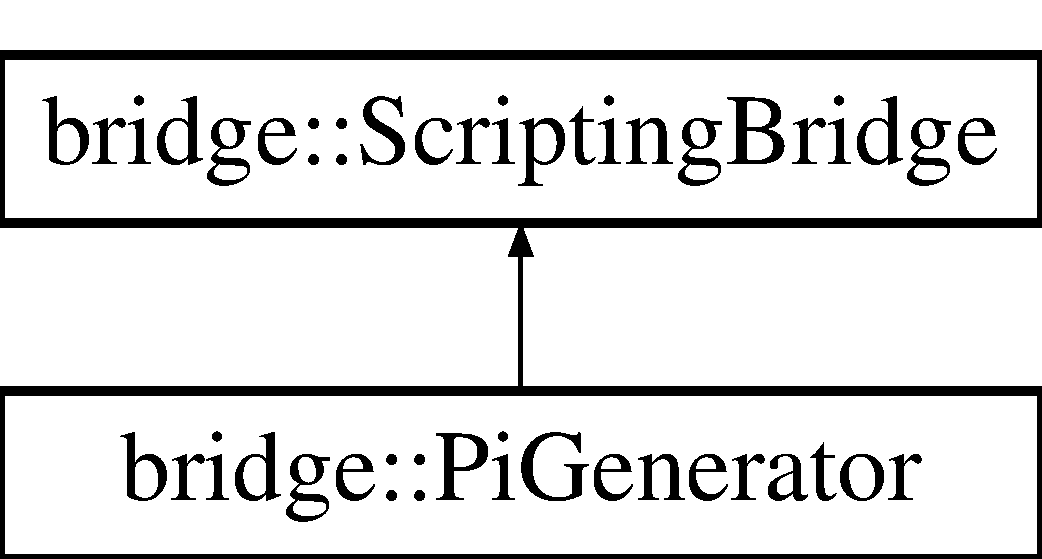
\includegraphics[height=2cm]{classbridge_1_1_pi_generator}
\end{center}
\end{figure}
\subsection*{Public Member Functions}
\begin{DoxyCompactItemize}
\item 
\hyperlink{classbridge_1_1_pi_generator_a1f76a8c23b9f71c440d8a86e91f9b177}{PiGenerator} (NPP npp)
\item 
\hyperlink{classbridge_1_1_pi_generator_ae2369ad51a1680d21ff001404a8a84b5}{$\sim$PiGenerator} ()
\item 
bool \hyperlink{classbridge_1_1_pi_generator_a7d6deb8aca71aa7c3692894f489afd30}{Paint} ()
\item 
bool \hyperlink{classbridge_1_1_pi_generator_a756bd50f86283c0970abbb1ce0d0a322}{quit} () const 
\item 
double \hyperlink{classbridge_1_1_pi_generator_ac477983021d094e067edb005af305212}{pi} () const 
\item 
void $\ast$ \hyperlink{classbridge_1_1_pi_generator_a51490d5ee5ac9c1beb10459643f7083a}{pixels} () const 
\item 
int \hyperlink{classbridge_1_1_pi_generator_ab96bd1df955862228ca1c2a42344debc}{width} () const 
\item 
int \hyperlink{classbridge_1_1_pi_generator_a4f079f180ee84d53cab6df3f5baf7492}{height} () const 
\end{DoxyCompactItemize}
\subsection*{Protected Member Functions}
\begin{DoxyCompactItemize}
\item 
void \hyperlink{classbridge_1_1_pi_generator_aa5be4efa2d7fe286582ccec734619db4}{CreateContext} ()
\item 
void \hyperlink{classbridge_1_1_pi_generator_ad0299e34e6e407bdb4b10dd6b26772e1}{DestroyContext} ()
\end{DoxyCompactItemize}
\subsection*{Static Protected Member Functions}
\begin{DoxyCompactItemize}
\item 
static void $\ast$ \hyperlink{classbridge_1_1_pi_generator_a869dcf4a6fb5598feece0d4d184caf23}{pi} (void $\ast$param)
\end{DoxyCompactItemize}
\subsection*{Protected Attributes}
\begin{DoxyCompactItemize}
\item 
bool \hyperlink{classbridge_1_1_pi_generator_a682f8e27a788cb81f1b862b02e6ab127}{quit\_\-}
\item 
double \hyperlink{classbridge_1_1_pi_generator_a3d35a8b7e364db2572a1e3e983ff5053}{pi\_\-}
\end{DoxyCompactItemize}


\subsection{Detailed Description}


Definition at line 17 of file pi\_\-generator.h.



\subsection{Constructor \& Destructor Documentation}
\hypertarget{classbridge_1_1_pi_generator_a1f76a8c23b9f71c440d8a86e91f9b177}{
\index{bridge::PiGenerator@{bridge::PiGenerator}!PiGenerator@{PiGenerator}}
\index{PiGenerator@{PiGenerator}!bridge::PiGenerator@{bridge::PiGenerator}}
\subsubsection[{PiGenerator}]{\setlength{\rightskip}{0pt plus 5cm}bridge::PiGenerator::PiGenerator (NPP {\em npp})}}
\label{classbridge_1_1_pi_generator_a1f76a8c23b9f71c440d8a86e91f9b177}


Definition at line 33 of file pi\_\-generator.cc.

\hypertarget{classbridge_1_1_pi_generator_ae2369ad51a1680d21ff001404a8a84b5}{
\index{bridge::PiGenerator@{bridge::PiGenerator}!$\sim$PiGenerator@{$\sim$PiGenerator}}
\index{$\sim$PiGenerator@{$\sim$PiGenerator}!bridge::PiGenerator@{bridge::PiGenerator}}
\subsubsection[{$\sim$PiGenerator}]{\setlength{\rightskip}{0pt plus 5cm}bridge::PiGenerator::$\sim$PiGenerator ()}}
\label{classbridge_1_1_pi_generator_ae2369ad51a1680d21ff001404a8a84b5}


Definition at line 40 of file pi\_\-generator.cc.



\subsection{Member Function Documentation}
\hypertarget{classbridge_1_1_pi_generator_aa5be4efa2d7fe286582ccec734619db4}{
\index{bridge::PiGenerator@{bridge::PiGenerator}!CreateContext@{CreateContext}}
\index{CreateContext@{CreateContext}!bridge::PiGenerator@{bridge::PiGenerator}}
\subsubsection[{CreateContext}]{\setlength{\rightskip}{0pt plus 5cm}void bridge::PiGenerator::CreateContext ()\hspace{0.3cm}{\ttfamily  \mbox{[}protected\mbox{]}}}}
\label{classbridge_1_1_pi_generator_aa5be4efa2d7fe286582ccec734619db4}


Reimplemented from \hyperlink{classbridge_1_1_scripting_bridge_a1ebec17acf6dfcd03462eee8fec9406e}{bridge::ScriptingBridge}.

\hypertarget{classbridge_1_1_pi_generator_ad0299e34e6e407bdb4b10dd6b26772e1}{
\index{bridge::PiGenerator@{bridge::PiGenerator}!DestroyContext@{DestroyContext}}
\index{DestroyContext@{DestroyContext}!bridge::PiGenerator@{bridge::PiGenerator}}
\subsubsection[{DestroyContext}]{\setlength{\rightskip}{0pt plus 5cm}void bridge::PiGenerator::DestroyContext ()\hspace{0.3cm}{\ttfamily  \mbox{[}protected\mbox{]}}}}
\label{classbridge_1_1_pi_generator_ad0299e34e6e407bdb4b10dd6b26772e1}


Definition at line 78 of file pi\_\-generator.cc.

\hypertarget{classbridge_1_1_pi_generator_a4f079f180ee84d53cab6df3f5baf7492}{
\index{bridge::PiGenerator@{bridge::PiGenerator}!height@{height}}
\index{height@{height}!bridge::PiGenerator@{bridge::PiGenerator}}
\subsubsection[{height}]{\setlength{\rightskip}{0pt plus 5cm}int bridge::PiGenerator::height () const\hspace{0.3cm}{\ttfamily  \mbox{[}inline\mbox{]}}}}
\label{classbridge_1_1_pi_generator_a4f079f180ee84d53cab6df3f5baf7492}


Definition at line 37 of file pi\_\-generator.h.

\hypertarget{classbridge_1_1_pi_generator_a7d6deb8aca71aa7c3692894f489afd30}{
\index{bridge::PiGenerator@{bridge::PiGenerator}!Paint@{Paint}}
\index{Paint@{Paint}!bridge::PiGenerator@{bridge::PiGenerator}}
\subsubsection[{Paint}]{\setlength{\rightskip}{0pt plus 5cm}bool bridge::PiGenerator::Paint ()}}
\label{classbridge_1_1_pi_generator_a7d6deb8aca71aa7c3692894f489afd30}


Definition at line 51 of file pi\_\-generator.cc.

\hypertarget{classbridge_1_1_pi_generator_a869dcf4a6fb5598feece0d4d184caf23}{
\index{bridge::PiGenerator@{bridge::PiGenerator}!pi@{pi}}
\index{pi@{pi}!bridge::PiGenerator@{bridge::PiGenerator}}
\subsubsection[{pi}]{\setlength{\rightskip}{0pt plus 5cm}void $\ast$ bridge::PiGenerator::pi (void $\ast$ {\em param})\hspace{0.3cm}{\ttfamily  \mbox{[}static, protected\mbox{]}}}}
\label{classbridge_1_1_pi_generator_a869dcf4a6fb5598feece0d4d184caf23}


Definition at line 89 of file pi\_\-generator.cc.

\hypertarget{classbridge_1_1_pi_generator_ac477983021d094e067edb005af305212}{
\index{bridge::PiGenerator@{bridge::PiGenerator}!pi@{pi}}
\index{pi@{pi}!bridge::PiGenerator@{bridge::PiGenerator}}
\subsubsection[{pi}]{\setlength{\rightskip}{0pt plus 5cm}double bridge::PiGenerator::pi () const\hspace{0.3cm}{\ttfamily  \mbox{[}inline\mbox{]}}}}
\label{classbridge_1_1_pi_generator_ac477983021d094e067edb005af305212}


Definition at line 28 of file pi\_\-generator.h.

\hypertarget{classbridge_1_1_pi_generator_a51490d5ee5ac9c1beb10459643f7083a}{
\index{bridge::PiGenerator@{bridge::PiGenerator}!pixels@{pixels}}
\index{pixels@{pixels}!bridge::PiGenerator@{bridge::PiGenerator}}
\subsubsection[{pixels}]{\setlength{\rightskip}{0pt plus 5cm}void$\ast$ bridge::PiGenerator::pixels () const\hspace{0.3cm}{\ttfamily  \mbox{[}inline\mbox{]}}}}
\label{classbridge_1_1_pi_generator_a51490d5ee5ac9c1beb10459643f7083a}


Definition at line 31 of file pi\_\-generator.h.

\hypertarget{classbridge_1_1_pi_generator_a756bd50f86283c0970abbb1ce0d0a322}{
\index{bridge::PiGenerator@{bridge::PiGenerator}!quit@{quit}}
\index{quit@{quit}!bridge::PiGenerator@{bridge::PiGenerator}}
\subsubsection[{quit}]{\setlength{\rightskip}{0pt plus 5cm}bool bridge::PiGenerator::quit () const\hspace{0.3cm}{\ttfamily  \mbox{[}inline\mbox{]}}}}
\label{classbridge_1_1_pi_generator_a756bd50f86283c0970abbb1ce0d0a322}


Definition at line 25 of file pi\_\-generator.h.

\hypertarget{classbridge_1_1_pi_generator_ab96bd1df955862228ca1c2a42344debc}{
\index{bridge::PiGenerator@{bridge::PiGenerator}!width@{width}}
\index{width@{width}!bridge::PiGenerator@{bridge::PiGenerator}}
\subsubsection[{width}]{\setlength{\rightskip}{0pt plus 5cm}int bridge::PiGenerator::width () const\hspace{0.3cm}{\ttfamily  \mbox{[}inline\mbox{]}}}}
\label{classbridge_1_1_pi_generator_ab96bd1df955862228ca1c2a42344debc}


Definition at line 34 of file pi\_\-generator.h.



\subsection{Member Data Documentation}
\hypertarget{classbridge_1_1_pi_generator_a3d35a8b7e364db2572a1e3e983ff5053}{
\index{bridge::PiGenerator@{bridge::PiGenerator}!pi\_\-@{pi\_\-}}
\index{pi\_\-@{pi\_\-}!bridge::PiGenerator@{bridge::PiGenerator}}
\subsubsection[{pi\_\-}]{\setlength{\rightskip}{0pt plus 5cm}double {\bf bridge::PiGenerator::pi\_\-}\hspace{0.3cm}{\ttfamily  \mbox{[}protected\mbox{]}}}}
\label{classbridge_1_1_pi_generator_a3d35a8b7e364db2572a1e3e983ff5053}


Definition at line 50 of file pi\_\-generator.h.

\hypertarget{classbridge_1_1_pi_generator_a682f8e27a788cb81f1b862b02e6ab127}{
\index{bridge::PiGenerator@{bridge::PiGenerator}!quit\_\-@{quit\_\-}}
\index{quit\_\-@{quit\_\-}!bridge::PiGenerator@{bridge::PiGenerator}}
\subsubsection[{quit\_\-}]{\setlength{\rightskip}{0pt plus 5cm}bool {\bf bridge::PiGenerator::quit\_\-}\hspace{0.3cm}{\ttfamily  \mbox{[}protected\mbox{]}}}}
\label{classbridge_1_1_pi_generator_a682f8e27a788cb81f1b862b02e6ab127}


Definition at line 49 of file pi\_\-generator.h.



The documentation for this class was generated from the following files:\begin{DoxyCompactItemize}
\item 
/home/derek/dev/crml/crml/test/pi\_\-generator\_\-crml/\hyperlink{pi__generator__crml_2pi__generator_8h}{pi\_\-generator.h}\item 
/home/derek/dev/crml/crml/test/pi\_\-generator\_\-crml/\hyperlink{pi__generator__crml_2pi__generator_8cc}{pi\_\-generator.cc}\end{DoxyCompactItemize}

\hypertarget{classhttpd_1_1_quittable_h_t_t_p_handler}{
\section{httpd::QuittableHTTPHandler Class Reference}
\label{classhttpd_1_1_quittable_h_t_t_p_handler}\index{httpd::QuittableHTTPHandler@{httpd::QuittableHTTPHandler}}
}
\subsection*{Public Member Functions}
\begin{DoxyCompactItemize}
\item 
def \hyperlink{classhttpd_1_1_quittable_h_t_t_p_handler_addc36268dbff72748204a5baae7a6e5b}{do\_\-GET}
\item 
def \hyperlink{classhttpd_1_1_quittable_h_t_t_p_handler_addc36268dbff72748204a5baae7a6e5b}{do\_\-GET}
\end{DoxyCompactItemize}


\subsection{Detailed Description}


Definition at line 73 of file httpd.py.



\subsection{Member Function Documentation}
\hypertarget{classhttpd_1_1_quittable_h_t_t_p_handler_addc36268dbff72748204a5baae7a6e5b}{
\index{httpd::QuittableHTTPHandler@{httpd::QuittableHTTPHandler}!do\_\-GET@{do\_\-GET}}
\index{do\_\-GET@{do\_\-GET}!httpd::QuittableHTTPHandler@{httpd::QuittableHTTPHandler}}
\subsubsection[{do\_\-GET}]{\setlength{\rightskip}{0pt plus 5cm}def httpd::QuittableHTTPHandler::do\_\-GET ( {\em self})}}
\label{classhttpd_1_1_quittable_h_t_t_p_handler_addc36268dbff72748204a5baae7a6e5b}


Definition at line 74 of file httpd.py.

\hypertarget{classhttpd_1_1_quittable_h_t_t_p_handler_addc36268dbff72748204a5baae7a6e5b}{
\index{httpd::QuittableHTTPHandler@{httpd::QuittableHTTPHandler}!do\_\-GET@{do\_\-GET}}
\index{do\_\-GET@{do\_\-GET}!httpd::QuittableHTTPHandler@{httpd::QuittableHTTPHandler}}
\subsubsection[{do\_\-GET}]{\setlength{\rightskip}{0pt plus 5cm}def httpd::QuittableHTTPHandler::do\_\-GET ( {\em self})}}
\label{classhttpd_1_1_quittable_h_t_t_p_handler_addc36268dbff72748204a5baae7a6e5b}


Definition at line 74 of file httpd.py.



The documentation for this class was generated from the following files:\begin{DoxyCompactItemize}
\item 
/home/derek/dev/crml/crml/src/web/\hyperlink{src_2web_2httpd_8py}{httpd.py}\item 
/home/derek/dev/crml/crml/test/\hyperlink{test_2httpd_8py}{httpd.py}\end{DoxyCompactItemize}

\hypertarget{classhttpd_1_1_quittable_h_t_t_p_server}{
\section{httpd::QuittableHTTPServer Class Reference}
\label{classhttpd_1_1_quittable_h_t_t_p_server}\index{httpd::QuittableHTTPServer@{httpd::QuittableHTTPServer}}
}
\subsection*{Public Member Functions}
\begin{DoxyCompactItemize}
\item 
def \hyperlink{classhttpd_1_1_quittable_h_t_t_p_server_ad7da0003b17805e7e629fa09a3a8f187}{serve\_\-forever}
\item 
def \hyperlink{classhttpd_1_1_quittable_h_t_t_p_server_a7d527531f10ecbcb1db670cf816bbcbd}{shutdown}
\end{DoxyCompactItemize}
\subsection*{Public Attributes}
\begin{DoxyCompactItemize}
\item 
\hyperlink{classhttpd_1_1_quittable_h_t_t_p_server_a72e565dcba798dfd43d18268e92075a8}{is\_\-running}
\end{DoxyCompactItemize}


\subsection{Detailed Description}


Definition at line 50 of file httpd.py.



\subsection{Member Function Documentation}
\hypertarget{classhttpd_1_1_quittable_h_t_t_p_server_ad7da0003b17805e7e629fa09a3a8f187}{
\index{httpd::QuittableHTTPServer@{httpd::QuittableHTTPServer}!serve\_\-forever@{serve\_\-forever}}
\index{serve\_\-forever@{serve\_\-forever}!httpd::QuittableHTTPServer@{httpd::QuittableHTTPServer}}
\subsubsection[{serve\_\-forever}]{\setlength{\rightskip}{0pt plus 5cm}def httpd::QuittableHTTPServer::serve\_\-forever ( {\em self})}}
\label{classhttpd_1_1_quittable_h_t_t_p_server_ad7da0003b17805e7e629fa09a3a8f187}


Definition at line 51 of file httpd.py.

\hypertarget{classhttpd_1_1_quittable_h_t_t_p_server_a7d527531f10ecbcb1db670cf816bbcbd}{
\index{httpd::QuittableHTTPServer@{httpd::QuittableHTTPServer}!shutdown@{shutdown}}
\index{shutdown@{shutdown}!httpd::QuittableHTTPServer@{httpd::QuittableHTTPServer}}
\subsubsection[{shutdown}]{\setlength{\rightskip}{0pt plus 5cm}def httpd::QuittableHTTPServer::shutdown ( {\em self})}}
\label{classhttpd_1_1_quittable_h_t_t_p_server_a7d527531f10ecbcb1db670cf816bbcbd}


Definition at line 56 of file httpd.py.



\subsection{Member Data Documentation}
\hypertarget{classhttpd_1_1_quittable_h_t_t_p_server_a72e565dcba798dfd43d18268e92075a8}{
\index{httpd::QuittableHTTPServer@{httpd::QuittableHTTPServer}!is\_\-running@{is\_\-running}}
\index{is\_\-running@{is\_\-running}!httpd::QuittableHTTPServer@{httpd::QuittableHTTPServer}}
\subsubsection[{is\_\-running}]{\setlength{\rightskip}{0pt plus 5cm}{\bf httpd::QuittableHTTPServer::is\_\-running}}}
\label{classhttpd_1_1_quittable_h_t_t_p_server_a72e565dcba798dfd43d18268e92075a8}


Definition at line 52 of file httpd.py.



The documentation for this class was generated from the following file:\begin{DoxyCompactItemize}
\item 
/home/derek/dev/cell-\/grid-\/game/nacl/crml/crml/web/\hyperlink{httpd_8py}{httpd.py}\end{DoxyCompactItemize}

\hypertarget{class_scripting_bridge}{
\section{ScriptingBridge Class Reference}
\label{class_scripting_bridge}\index{ScriptingBridge@{ScriptingBridge}}
}


{\ttfamily \#include $<$scripting\_\-bridge.h$>$}

\subsection*{Public Types}
\begin{DoxyCompactItemize}
\item 
typedef bool(ScriptingBridge::$\ast$ \hyperlink{class_scripting_bridge_a53de202658094d3663f4c330bb096291}{Method} )(const NPVariant $\ast$args, uint32\_\-t arg\_\-count, NPVariant $\ast$result)
\item 
typedef bool(ScriptingBridge::$\ast$ \hyperlink{class_scripting_bridge_afe9032a0f312e1f440f8fed19ffe64d7}{Property} )(NPVariant $\ast$result)
\end{DoxyCompactItemize}
\subsection*{Public Member Functions}
\begin{DoxyCompactItemize}
\item 
\hyperlink{class_scripting_bridge_ae743ff1b8ffce6889a86a73500fd0da1}{ScriptingBridge} (NPP npp)
\item 
virtual \hyperlink{class_scripting_bridge_a8e85d3e7803f38a7182ac2be45d45a4d}{$\sim$ScriptingBridge} ()
\item 
virtual void \hyperlink{class_scripting_bridge_a9ee60d17b25c9b968315b6a12a55d841}{Invalidate} ()
\item 
virtual bool \hyperlink{class_scripting_bridge_a7eafa4200bb68bf6632c6b635aa4953f}{HasMethod} (NPIdentifier name)
\item 
virtual bool \hyperlink{class_scripting_bridge_a8c6d388d7c7e1660b267013143d0cdf5}{Invoke} (NPIdentifier name, const NPVariant $\ast$args, uint32\_\-t arg\_\-count, NPVariant $\ast$result)
\item 
virtual bool \hyperlink{class_scripting_bridge_a9045116428a296ea7073ffbdce73d80e}{InvokeDefault} (const NPVariant $\ast$args, uint32\_\-t arg\_\-count, NPVariant $\ast$result)
\item 
virtual bool \hyperlink{class_scripting_bridge_a425cfcd308f30736bf936f2e0aca1d6c}{HasProperty} (NPIdentifier name)
\item 
virtual bool \hyperlink{class_scripting_bridge_ac971765b22d611a0e0661a523650885d}{GetProperty} (NPIdentifier name, NPVariant $\ast$result)
\item 
virtual bool \hyperlink{class_scripting_bridge_aee815679c5b398c1d288322d6b21e81d}{SetProperty} (NPIdentifier name, const NPVariant $\ast$value)
\item 
virtual bool \hyperlink{class_scripting_bridge_a4948d9d87de0dc58627c8b377356df34}{RemoveProperty} (NPIdentifier name)
\end{DoxyCompactItemize}
\subsection*{Static Public Member Functions}
\begin{DoxyCompactItemize}
\item 
static bool \hyperlink{class_scripting_bridge_a744b9ecf0b3f4a39aa51c85b1ee5d5e9}{InitializeIdentifiers} ()
\end{DoxyCompactItemize}
\subsection*{Static Public Attributes}
\begin{DoxyCompactItemize}
\item 
static NPClass \hyperlink{class_scripting_bridge_a4fcbbbaf7a6d91a2766066fa2cb2236b}{np\_\-class}
\end{DoxyCompactItemize}


\subsection{Detailed Description}


Definition at line 11 of file scripting\_\-bridge.h.



\subsection{Member Typedef Documentation}
\hypertarget{class_scripting_bridge_a53de202658094d3663f4c330bb096291}{
\index{ScriptingBridge@{ScriptingBridge}!Method@{Method}}
\index{Method@{Method}!ScriptingBridge@{ScriptingBridge}}
\subsubsection[{Method}]{\setlength{\rightskip}{0pt plus 5cm}typedef bool(ScriptingBridge::$\ast$ {\bf ScriptingBridge::Method})(const NPVariant $\ast$args, uint32\_\-t arg\_\-count, NPVariant $\ast$result)}}
\label{class_scripting_bridge_a53de202658094d3663f4c330bb096291}


Definition at line 13 of file scripting\_\-bridge.h.

\hypertarget{class_scripting_bridge_afe9032a0f312e1f440f8fed19ffe64d7}{
\index{ScriptingBridge@{ScriptingBridge}!Property@{Property}}
\index{Property@{Property}!ScriptingBridge@{ScriptingBridge}}
\subsubsection[{Property}]{\setlength{\rightskip}{0pt plus 5cm}typedef bool(ScriptingBridge::$\ast$ {\bf ScriptingBridge::Property})(NPVariant $\ast$result)}}
\label{class_scripting_bridge_afe9032a0f312e1f440f8fed19ffe64d7}


Definition at line 16 of file scripting\_\-bridge.h.



\subsection{Constructor \& Destructor Documentation}
\hypertarget{class_scripting_bridge_ae743ff1b8ffce6889a86a73500fd0da1}{
\index{ScriptingBridge@{ScriptingBridge}!ScriptingBridge@{ScriptingBridge}}
\index{ScriptingBridge@{ScriptingBridge}!ScriptingBridge@{ScriptingBridge}}
\subsubsection[{ScriptingBridge}]{\setlength{\rightskip}{0pt plus 5cm}ScriptingBridge::ScriptingBridge (NPP {\em npp})\hspace{0.3cm}{\ttfamily  \mbox{[}inline, explicit\mbox{]}}}}
\label{class_scripting_bridge_ae743ff1b8ffce6889a86a73500fd0da1}


Definition at line 18 of file scripting\_\-bridge.h.

\hypertarget{class_scripting_bridge_a8e85d3e7803f38a7182ac2be45d45a4d}{
\index{ScriptingBridge@{ScriptingBridge}!$\sim$ScriptingBridge@{$\sim$ScriptingBridge}}
\index{$\sim$ScriptingBridge@{$\sim$ScriptingBridge}!ScriptingBridge@{ScriptingBridge}}
\subsubsection[{$\sim$ScriptingBridge}]{\setlength{\rightskip}{0pt plus 5cm}virtual ScriptingBridge::$\sim$ScriptingBridge ()\hspace{0.3cm}{\ttfamily  \mbox{[}virtual\mbox{]}}}}
\label{class_scripting_bridge_a8e85d3e7803f38a7182ac2be45d45a4d}


\subsection{Member Function Documentation}
\hypertarget{class_scripting_bridge_ac971765b22d611a0e0661a523650885d}{
\index{ScriptingBridge@{ScriptingBridge}!GetProperty@{GetProperty}}
\index{GetProperty@{GetProperty}!ScriptingBridge@{ScriptingBridge}}
\subsubsection[{GetProperty}]{\setlength{\rightskip}{0pt plus 5cm}virtual bool ScriptingBridge::GetProperty (NPIdentifier {\em name}, \/  NPVariant $\ast$ {\em result})\hspace{0.3cm}{\ttfamily  \mbox{[}virtual\mbox{]}}}}
\label{class_scripting_bridge_ac971765b22d611a0e0661a523650885d}
\hypertarget{class_scripting_bridge_a7eafa4200bb68bf6632c6b635aa4953f}{
\index{ScriptingBridge@{ScriptingBridge}!HasMethod@{HasMethod}}
\index{HasMethod@{HasMethod}!ScriptingBridge@{ScriptingBridge}}
\subsubsection[{HasMethod}]{\setlength{\rightskip}{0pt plus 5cm}virtual bool ScriptingBridge::HasMethod (NPIdentifier {\em name})\hspace{0.3cm}{\ttfamily  \mbox{[}virtual\mbox{]}}}}
\label{class_scripting_bridge_a7eafa4200bb68bf6632c6b635aa4953f}
\hypertarget{class_scripting_bridge_a425cfcd308f30736bf936f2e0aca1d6c}{
\index{ScriptingBridge@{ScriptingBridge}!HasProperty@{HasProperty}}
\index{HasProperty@{HasProperty}!ScriptingBridge@{ScriptingBridge}}
\subsubsection[{HasProperty}]{\setlength{\rightskip}{0pt plus 5cm}virtual bool ScriptingBridge::HasProperty (NPIdentifier {\em name})\hspace{0.3cm}{\ttfamily  \mbox{[}virtual\mbox{]}}}}
\label{class_scripting_bridge_a425cfcd308f30736bf936f2e0aca1d6c}
\hypertarget{class_scripting_bridge_a744b9ecf0b3f4a39aa51c85b1ee5d5e9}{
\index{ScriptingBridge@{ScriptingBridge}!InitializeIdentifiers@{InitializeIdentifiers}}
\index{InitializeIdentifiers@{InitializeIdentifiers}!ScriptingBridge@{ScriptingBridge}}
\subsubsection[{InitializeIdentifiers}]{\setlength{\rightskip}{0pt plus 5cm}static bool ScriptingBridge::InitializeIdentifiers ()\hspace{0.3cm}{\ttfamily  \mbox{[}static\mbox{]}}}}
\label{class_scripting_bridge_a744b9ecf0b3f4a39aa51c85b1ee5d5e9}
\hypertarget{class_scripting_bridge_a9ee60d17b25c9b968315b6a12a55d841}{
\index{ScriptingBridge@{ScriptingBridge}!Invalidate@{Invalidate}}
\index{Invalidate@{Invalidate}!ScriptingBridge@{ScriptingBridge}}
\subsubsection[{Invalidate}]{\setlength{\rightskip}{0pt plus 5cm}virtual void ScriptingBridge::Invalidate ()\hspace{0.3cm}{\ttfamily  \mbox{[}virtual\mbox{]}}}}
\label{class_scripting_bridge_a9ee60d17b25c9b968315b6a12a55d841}
\hypertarget{class_scripting_bridge_a8c6d388d7c7e1660b267013143d0cdf5}{
\index{ScriptingBridge@{ScriptingBridge}!Invoke@{Invoke}}
\index{Invoke@{Invoke}!ScriptingBridge@{ScriptingBridge}}
\subsubsection[{Invoke}]{\setlength{\rightskip}{0pt plus 5cm}virtual bool ScriptingBridge::Invoke (NPIdentifier {\em name}, \/  const NPVariant $\ast$ {\em args}, \/  uint32\_\-t {\em arg\_\-count}, \/  NPVariant $\ast$ {\em result})\hspace{0.3cm}{\ttfamily  \mbox{[}virtual\mbox{]}}}}
\label{class_scripting_bridge_a8c6d388d7c7e1660b267013143d0cdf5}
\hypertarget{class_scripting_bridge_a9045116428a296ea7073ffbdce73d80e}{
\index{ScriptingBridge@{ScriptingBridge}!InvokeDefault@{InvokeDefault}}
\index{InvokeDefault@{InvokeDefault}!ScriptingBridge@{ScriptingBridge}}
\subsubsection[{InvokeDefault}]{\setlength{\rightskip}{0pt plus 5cm}virtual bool ScriptingBridge::InvokeDefault (const NPVariant $\ast$ {\em args}, \/  uint32\_\-t {\em arg\_\-count}, \/  NPVariant $\ast$ {\em result})\hspace{0.3cm}{\ttfamily  \mbox{[}virtual\mbox{]}}}}
\label{class_scripting_bridge_a9045116428a296ea7073ffbdce73d80e}
\hypertarget{class_scripting_bridge_a4948d9d87de0dc58627c8b377356df34}{
\index{ScriptingBridge@{ScriptingBridge}!RemoveProperty@{RemoveProperty}}
\index{RemoveProperty@{RemoveProperty}!ScriptingBridge@{ScriptingBridge}}
\subsubsection[{RemoveProperty}]{\setlength{\rightskip}{0pt plus 5cm}virtual bool ScriptingBridge::RemoveProperty (NPIdentifier {\em name})\hspace{0.3cm}{\ttfamily  \mbox{[}virtual\mbox{]}}}}
\label{class_scripting_bridge_a4948d9d87de0dc58627c8b377356df34}
\hypertarget{class_scripting_bridge_aee815679c5b398c1d288322d6b21e81d}{
\index{ScriptingBridge@{ScriptingBridge}!SetProperty@{SetProperty}}
\index{SetProperty@{SetProperty}!ScriptingBridge@{ScriptingBridge}}
\subsubsection[{SetProperty}]{\setlength{\rightskip}{0pt plus 5cm}virtual bool ScriptingBridge::SetProperty (NPIdentifier {\em name}, \/  const NPVariant $\ast$ {\em value})\hspace{0.3cm}{\ttfamily  \mbox{[}virtual\mbox{]}}}}
\label{class_scripting_bridge_aee815679c5b398c1d288322d6b21e81d}


\subsection{Member Data Documentation}
\hypertarget{class_scripting_bridge_a4fcbbbaf7a6d91a2766066fa2cb2236b}{
\index{ScriptingBridge@{ScriptingBridge}!np\_\-class@{np\_\-class}}
\index{np\_\-class@{np\_\-class}!ScriptingBridge@{ScriptingBridge}}
\subsubsection[{np\_\-class}]{\setlength{\rightskip}{0pt plus 5cm}NPClass {\bf ScriptingBridge::np\_\-class}\hspace{0.3cm}{\ttfamily  \mbox{[}static\mbox{]}}}}
\label{class_scripting_bridge_a4fcbbbaf7a6d91a2766066fa2cb2236b}


Definition at line 39 of file scripting\_\-bridge.h.



The documentation for this class was generated from the following file:\begin{DoxyCompactItemize}
\item 
/home/derek/dev/crml/crml/src/sys/\hyperlink{src_2sys_2scripting__bridge_8h}{scripting\_\-bridge.h}\end{DoxyCompactItemize}

\hypertarget{classbridge_1_1_scripting_bridge}{
\section{bridge::ScriptingBridge Class Reference}
\label{classbridge_1_1_scripting_bridge}\index{bridge::ScriptingBridge@{bridge::ScriptingBridge}}
}


{\ttfamily \#include $<$scripting\_\-bridge.h$>$}

Inheritance diagram for bridge::ScriptingBridge:\begin{figure}[H]
\begin{center}
\leavevmode
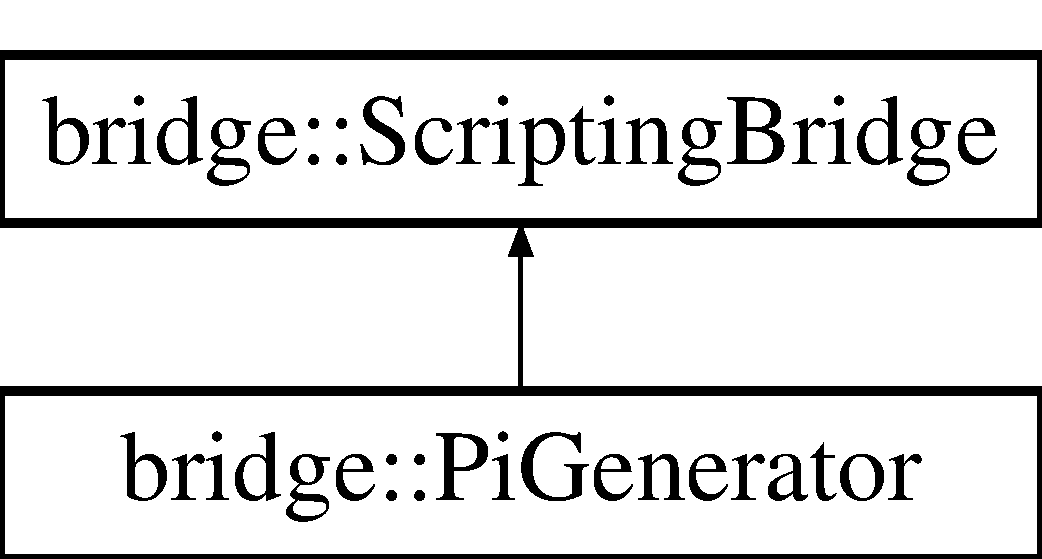
\includegraphics[height=2cm]{classbridge_1_1_scripting_bridge}
\end{center}
\end{figure}
\subsection*{Public Types}
\begin{DoxyCompactItemize}
\item 
typedef bool(ScriptingBridge::$\ast$ \hyperlink{classbridge_1_1_scripting_bridge_aa2d60d52b4e91aa7659850b73f393727}{Method} )(const NPVariant $\ast$args, uint32\_\-t arg\_\-count, NPVariant $\ast$result)
\item 
typedef bool(ScriptingBridge::$\ast$ \hyperlink{classbridge_1_1_scripting_bridge_a9063ac1ad0b4e1a439e954e7a505057d}{Property} )(NPVariant $\ast$result)
\item 
typedef bool(ScriptingBridge::$\ast$ \hyperlink{classbridge_1_1_scripting_bridge_aa2d60d52b4e91aa7659850b73f393727}{Method} )(const NPVariant $\ast$args, uint32\_\-t arg\_\-count, NPVariant $\ast$result)
\item 
typedef bool(ScriptingBridge::$\ast$ \hyperlink{classbridge_1_1_scripting_bridge_a9063ac1ad0b4e1a439e954e7a505057d}{Property} )(NPVariant $\ast$result)
\end{DoxyCompactItemize}
\subsection*{Public Member Functions}
\begin{DoxyCompactItemize}
\item 
\hyperlink{classbridge_1_1_scripting_bridge_a9f6cceea3738d76e33f47ba8ad5f72d9}{ScriptingBridge} (NPP npp)
\item 
virtual \hyperlink{classbridge_1_1_scripting_bridge_ae6c311b5f9ffa0a578c7d8e41fa9c23c}{$\sim$ScriptingBridge} ()
\item 
NPObject $\ast$ \hyperlink{classbridge_1_1_scripting_bridge_aab70aec1714cf92f28dca4afb87ad3b4}{GetScriptableObject} ()
\item 
NPError \hyperlink{classbridge_1_1_scripting_bridge_a6b2481696ae8caa5b322e7011c0228e0}{SetWindow} (NPWindow $\ast$window)
\item 
virtual void \hyperlink{classbridge_1_1_scripting_bridge_af00ea5a26438b33f976734a3432dfa9b}{Invalidate} ()
\item 
bool \hyperlink{classbridge_1_1_scripting_bridge_aa5f733424325e07c884397e3f301f01c}{AddMethod} (std::string, \hyperlink{classbridge_1_1_scripting_bridge_aa2d60d52b4e91aa7659850b73f393727}{Method}, NPIdentifier)
\item 
void \hyperlink{classbridge_1_1_scripting_bridge_a1ebec17acf6dfcd03462eee8fec9406e}{CreateContext} ()
\item 
virtual bool \hyperlink{classbridge_1_1_scripting_bridge_a1d614bb3696baef7c46332426ab7a0dc}{HasMethod} (NPIdentifier name)
\item 
virtual bool \hyperlink{classbridge_1_1_scripting_bridge_ad18d2af321b2cba1235876cf281295df}{Invoke} (NPIdentifier name, const NPVariant $\ast$args, uint32\_\-t arg\_\-count, NPVariant $\ast$result)
\item 
virtual bool \hyperlink{classbridge_1_1_scripting_bridge_a2cee828951db15b4cce1074e934c4f97}{InvokeDefault} (const NPVariant $\ast$args, uint32\_\-t arg\_\-count, NPVariant $\ast$result)
\item 
virtual bool \hyperlink{classbridge_1_1_scripting_bridge_aeed261c756896802f26632acfceba1d7}{HasProperty} (NPIdentifier name)
\item 
virtual bool \hyperlink{classbridge_1_1_scripting_bridge_afef889fc2ff5ccabefb713cf7ad5e056}{GetProperty} (NPIdentifier name, NPVariant $\ast$result)
\item 
virtual bool \hyperlink{classbridge_1_1_scripting_bridge_ae73ff0ec0f70dfcd0e22534c8281f3e3}{SetProperty} (NPIdentifier name, const NPVariant $\ast$value)
\item 
virtual bool \hyperlink{classbridge_1_1_scripting_bridge_a861437163b8291eb7b302ce8f778022d}{RemoveProperty} (NPIdentifier name)
\item 
bool \hyperlink{classbridge_1_1_scripting_bridge_a05f2a65b751d12e6aeaa00bfd91ef83f}{InitializeIdentifiers} ()
\item 
bool \hyperlink{classbridge_1_1_scripting_bridge_abfdee6fdc6c4f0cc6007425a14e8384e}{Paint} (const NPVariant $\ast$args, uint32\_\-t arg\_\-count, NPVariant $\ast$result)
\item 
bool \hyperlink{classbridge_1_1_scripting_bridge_ad09cd2cdc6df27d2c3f1ae6cda6d6958}{IsContextValid} ()
\item 
\hyperlink{classbridge_1_1_scripting_bridge_a9f6cceea3738d76e33f47ba8ad5f72d9}{ScriptingBridge} (NPP npp)
\item 
virtual \hyperlink{classbridge_1_1_scripting_bridge_ac47a1623f245bd55f96ea8cb007b24cb}{$\sim$ScriptingBridge} ()
\item 
virtual void \hyperlink{classbridge_1_1_scripting_bridge_a956430a5ae42b3e30c3e1b4655322061}{Invalidate} ()
\item 
bool \hyperlink{classbridge_1_1_scripting_bridge_a24f9e87d1beed97f7231010636d5af55}{AddMethod} (std::string, \hyperlink{classbridge_1_1_scripting_bridge_aa2d60d52b4e91aa7659850b73f393727}{Method}, NPIdentifier)
\item 
virtual bool \hyperlink{classbridge_1_1_scripting_bridge_af968e6487c5cc9e2566118634c0ab561}{HasMethod} (NPIdentifier name)
\item 
virtual bool \hyperlink{classbridge_1_1_scripting_bridge_a84f78dde38b524b61e72afebf7210483}{Invoke} (NPIdentifier name, const NPVariant $\ast$args, uint32\_\-t arg\_\-count, NPVariant $\ast$result)
\item 
virtual bool \hyperlink{classbridge_1_1_scripting_bridge_aec42e4cce5b1ff9187d98b88b07d11d3}{InvokeDefault} (const NPVariant $\ast$args, uint32\_\-t arg\_\-count, NPVariant $\ast$result)
\item 
virtual bool \hyperlink{classbridge_1_1_scripting_bridge_ad2cb9f2b860ba05a86c10f0824699e33}{HasProperty} (NPIdentifier name)
\item 
virtual bool \hyperlink{classbridge_1_1_scripting_bridge_aa7f5844674672f5872137ffee032427e}{GetProperty} (NPIdentifier name, NPVariant $\ast$result)
\item 
virtual bool \hyperlink{classbridge_1_1_scripting_bridge_a918981b30a60d961232e693e7ac15652}{SetProperty} (NPIdentifier name, const NPVariant $\ast$value)
\item 
virtual bool \hyperlink{classbridge_1_1_scripting_bridge_aeda2f5f7f5669003d573cdc2f3dc8fe8}{RemoveProperty} (NPIdentifier name)
\item 
bool \hyperlink{classbridge_1_1_scripting_bridge_a86ef6533d8f6ed9573890f017c6084d9}{InitializeIdentifiers} ()
\item 
bool \hyperlink{classbridge_1_1_scripting_bridge_a44eeaa7c1de524f8df7f218c1b53233b}{Paint} (const NPVariant $\ast$args, uint32\_\-t arg\_\-count, NPVariant $\ast$result)
\end{DoxyCompactItemize}
\subsection*{Static Public Attributes}
\begin{DoxyCompactItemize}
\item 
static NPClass \hyperlink{classbridge_1_1_scripting_bridge_a7a3e8318e9e315a116729cebceac5fd9}{np\_\-class}
\end{DoxyCompactItemize}
\subsection*{Protected Attributes}
\begin{DoxyCompactItemize}
\item 
NPP \hyperlink{classbridge_1_1_scripting_bridge_a122d088702ccb290a91a0cb1c507fbbe}{npp\_\-}
\item 
NPObject $\ast$ \hyperlink{classbridge_1_1_scripting_bridge_a59bc10d2500b138998dc973aee38039e}{window\_\-object\_\-}
\item 
NPObject $\ast$ \hyperlink{classbridge_1_1_scripting_bridge_a2f4a3c451a7056118de408d2d28d3936}{scriptable\_\-object\_\-}
\item 
NPDevice $\ast$ \hyperlink{classbridge_1_1_scripting_bridge_ad3a2e16a43b8a18b888ad880abd472c8}{device2d\_\-}
\item 
pthread\_\-t \hyperlink{classbridge_1_1_scripting_bridge_a58b77b4f3b290be810a88c67ba61db9d}{thread\_\-}
\item 
NPWindow $\ast$ \hyperlink{classbridge_1_1_scripting_bridge_ab23772fde4cbff4bc65520d589c8adac}{window\_\-}
\item 
NPDeviceContext2D \hyperlink{classbridge_1_1_scripting_bridge_ae8d47779a04203f58420dc3d9c88b063}{context2d\_\-}
\end{DoxyCompactItemize}
\subsection*{Static Protected Attributes}
\begin{DoxyCompactItemize}
\item 
static NPIdentifier \hyperlink{classbridge_1_1_scripting_bridge_af9fe1c1d57b6fb113b2e0da63128807d}{id\_\-paint}
\item 
static std::map$<$ NPIdentifier, \hyperlink{classbridge_1_1_scripting_bridge_aa2d60d52b4e91aa7659850b73f393727}{Method} $>$ $\ast$ \hyperlink{classbridge_1_1_scripting_bridge_a1057c4c6b923babcbc62a5732d2c3235}{method\_\-table}
\item 
static std::map$<$ NPIdentifier, \hyperlink{classbridge_1_1_scripting_bridge_a9063ac1ad0b4e1a439e954e7a505057d}{Property} $>$ $\ast$ \hyperlink{classbridge_1_1_scripting_bridge_a84c8336a6ba799945dfe31358d389a62}{property\_\-table}
\end{DoxyCompactItemize}


\subsection{Detailed Description}


Definition at line 15 of file scripting\_\-bridge.h.



\subsection{Member Typedef Documentation}
\hypertarget{classbridge_1_1_scripting_bridge_aa2d60d52b4e91aa7659850b73f393727}{
\index{bridge::ScriptingBridge@{bridge::ScriptingBridge}!Method@{Method}}
\index{Method@{Method}!bridge::ScriptingBridge@{bridge::ScriptingBridge}}
\subsubsection[{Method}]{\setlength{\rightskip}{0pt plus 5cm}typedef bool(ScriptingBridge::$\ast$ {\bf bridge::ScriptingBridge::Method})(const NPVariant $\ast$args, uint32\_\-t arg\_\-count, NPVariant $\ast$result)}}
\label{classbridge_1_1_scripting_bridge_aa2d60d52b4e91aa7659850b73f393727}


Definition at line 15 of file scripting\_\-bridge.h.

\hypertarget{classbridge_1_1_scripting_bridge_aa2d60d52b4e91aa7659850b73f393727}{
\index{bridge::ScriptingBridge@{bridge::ScriptingBridge}!Method@{Method}}
\index{Method@{Method}!bridge::ScriptingBridge@{bridge::ScriptingBridge}}
\subsubsection[{Method}]{\setlength{\rightskip}{0pt plus 5cm}typedef bool(ScriptingBridge::$\ast$ {\bf bridge::ScriptingBridge::Method})(const NPVariant $\ast$args, uint32\_\-t arg\_\-count, NPVariant $\ast$result)}}
\label{classbridge_1_1_scripting_bridge_aa2d60d52b4e91aa7659850b73f393727}


Definition at line 17 of file scripting\_\-bridge.h.

\hypertarget{classbridge_1_1_scripting_bridge_a9063ac1ad0b4e1a439e954e7a505057d}{
\index{bridge::ScriptingBridge@{bridge::ScriptingBridge}!Property@{Property}}
\index{Property@{Property}!bridge::ScriptingBridge@{bridge::ScriptingBridge}}
\subsubsection[{Property}]{\setlength{\rightskip}{0pt plus 5cm}typedef bool(ScriptingBridge::$\ast$ {\bf bridge::ScriptingBridge::Property})(NPVariant $\ast$result)}}
\label{classbridge_1_1_scripting_bridge_a9063ac1ad0b4e1a439e954e7a505057d}


Definition at line 19 of file scripting\_\-bridge.h.

\hypertarget{classbridge_1_1_scripting_bridge_a9063ac1ad0b4e1a439e954e7a505057d}{
\index{bridge::ScriptingBridge@{bridge::ScriptingBridge}!Property@{Property}}
\index{Property@{Property}!bridge::ScriptingBridge@{bridge::ScriptingBridge}}
\subsubsection[{Property}]{\setlength{\rightskip}{0pt plus 5cm}typedef bool(ScriptingBridge::$\ast$ {\bf bridge::ScriptingBridge::Property})(NPVariant $\ast$result)}}
\label{classbridge_1_1_scripting_bridge_a9063ac1ad0b4e1a439e954e7a505057d}


Definition at line 21 of file scripting\_\-bridge.h.



\subsection{Constructor \& Destructor Documentation}
\hypertarget{classbridge_1_1_scripting_bridge_a9f6cceea3738d76e33f47ba8ad5f72d9}{
\index{bridge::ScriptingBridge@{bridge::ScriptingBridge}!ScriptingBridge@{ScriptingBridge}}
\index{ScriptingBridge@{ScriptingBridge}!bridge::ScriptingBridge@{bridge::ScriptingBridge}}
\subsubsection[{ScriptingBridge}]{\setlength{\rightskip}{0pt plus 5cm}bridge::ScriptingBridge::ScriptingBridge (NPP {\em npp})\hspace{0.3cm}{\ttfamily  \mbox{[}inline, explicit\mbox{]}}}}
\label{classbridge_1_1_scripting_bridge_a9f6cceea3738d76e33f47ba8ad5f72d9}


Definition at line 23 of file scripting\_\-bridge.h.

\hypertarget{classbridge_1_1_scripting_bridge_ae6c311b5f9ffa0a578c7d8e41fa9c23c}{
\index{bridge::ScriptingBridge@{bridge::ScriptingBridge}!$\sim$ScriptingBridge@{$\sim$ScriptingBridge}}
\index{$\sim$ScriptingBridge@{$\sim$ScriptingBridge}!bridge::ScriptingBridge@{bridge::ScriptingBridge}}
\subsubsection[{$\sim$ScriptingBridge}]{\setlength{\rightskip}{0pt plus 5cm}ScriptingBridge::$\sim$ScriptingBridge ()\hspace{0.3cm}{\ttfamily  \mbox{[}virtual\mbox{]}}}}
\label{classbridge_1_1_scripting_bridge_ae6c311b5f9ffa0a578c7d8e41fa9c23c}


Definition at line 122 of file scripting\_\-bridge.cc.

\hypertarget{classbridge_1_1_scripting_bridge_a9f6cceea3738d76e33f47ba8ad5f72d9}{
\index{bridge::ScriptingBridge@{bridge::ScriptingBridge}!ScriptingBridge@{ScriptingBridge}}
\index{ScriptingBridge@{ScriptingBridge}!bridge::ScriptingBridge@{bridge::ScriptingBridge}}
\subsubsection[{ScriptingBridge}]{\setlength{\rightskip}{0pt plus 5cm}bridge::ScriptingBridge::ScriptingBridge (NPP {\em npp})\hspace{0.3cm}{\ttfamily  \mbox{[}inline, explicit\mbox{]}}}}
\label{classbridge_1_1_scripting_bridge_a9f6cceea3738d76e33f47ba8ad5f72d9}


Definition at line 21 of file scripting\_\-bridge.h.

\hypertarget{classbridge_1_1_scripting_bridge_ac47a1623f245bd55f96ea8cb007b24cb}{
\index{bridge::ScriptingBridge@{bridge::ScriptingBridge}!$\sim$ScriptingBridge@{$\sim$ScriptingBridge}}
\index{$\sim$ScriptingBridge@{$\sim$ScriptingBridge}!bridge::ScriptingBridge@{bridge::ScriptingBridge}}
\subsubsection[{$\sim$ScriptingBridge}]{\setlength{\rightskip}{0pt plus 5cm}virtual bridge::ScriptingBridge::$\sim$ScriptingBridge ()\hspace{0.3cm}{\ttfamily  \mbox{[}virtual\mbox{]}}}}
\label{classbridge_1_1_scripting_bridge_ac47a1623f245bd55f96ea8cb007b24cb}


\subsection{Member Function Documentation}
\hypertarget{classbridge_1_1_scripting_bridge_a24f9e87d1beed97f7231010636d5af55}{
\index{bridge::ScriptingBridge@{bridge::ScriptingBridge}!AddMethod@{AddMethod}}
\index{AddMethod@{AddMethod}!bridge::ScriptingBridge@{bridge::ScriptingBridge}}
\subsubsection[{AddMethod}]{\setlength{\rightskip}{0pt plus 5cm}bool bridge::ScriptingBridge::AddMethod (std::string, \/  {\bf Method}, \/  NPIdentifier)}}
\label{classbridge_1_1_scripting_bridge_a24f9e87d1beed97f7231010636d5af55}
\hypertarget{classbridge_1_1_scripting_bridge_aa5f733424325e07c884397e3f301f01c}{
\index{bridge::ScriptingBridge@{bridge::ScriptingBridge}!AddMethod@{AddMethod}}
\index{AddMethod@{AddMethod}!bridge::ScriptingBridge@{bridge::ScriptingBridge}}
\subsubsection[{AddMethod}]{\setlength{\rightskip}{0pt plus 5cm}bool ScriptingBridge::AddMethod (std::string {\em meth\_\-name}, \/  {\bf Method} {\em meth}, \/  NPIdentifier {\em meth\_\-id})}}
\label{classbridge_1_1_scripting_bridge_aa5f733424325e07c884397e3f301f01c}
Adds a method to the bridge, it will be visible to javascript. 
\begin{DoxyParams}{Parameters}
\item[{\em meth\_\-name}]The name of the method to be exposed \item[{\em meth}]A function pointer to the function to be called and associated with the meth\_\-name \end{DoxyParams}
\begin{DoxyReturn}{Returns}
a bool to indicate success or failure 
\end{DoxyReturn}


Definition at line 112 of file scripting\_\-bridge.cc.

\hypertarget{classbridge_1_1_scripting_bridge_a1ebec17acf6dfcd03462eee8fec9406e}{
\index{bridge::ScriptingBridge@{bridge::ScriptingBridge}!CreateContext@{CreateContext}}
\index{CreateContext@{CreateContext}!bridge::ScriptingBridge@{bridge::ScriptingBridge}}
\subsubsection[{CreateContext}]{\setlength{\rightskip}{0pt plus 5cm}void ScriptingBridge::CreateContext ()}}
\label{classbridge_1_1_scripting_bridge_a1ebec17acf6dfcd03462eee8fec9406e}


Reimplemented in \hyperlink{classbridge_1_1_pi_generator_aa5be4efa2d7fe286582ccec734619db4}{bridge::PiGenerator}.



Definition at line 67 of file scripting\_\-bridge.cc.

\hypertarget{classbridge_1_1_scripting_bridge_aa7f5844674672f5872137ffee032427e}{
\index{bridge::ScriptingBridge@{bridge::ScriptingBridge}!GetProperty@{GetProperty}}
\index{GetProperty@{GetProperty}!bridge::ScriptingBridge@{bridge::ScriptingBridge}}
\subsubsection[{GetProperty}]{\setlength{\rightskip}{0pt plus 5cm}virtual bool bridge::ScriptingBridge::GetProperty (NPIdentifier {\em name}, \/  NPVariant $\ast$ {\em result})\hspace{0.3cm}{\ttfamily  \mbox{[}virtual\mbox{]}}}}
\label{classbridge_1_1_scripting_bridge_aa7f5844674672f5872137ffee032427e}
\hypertarget{classbridge_1_1_scripting_bridge_afef889fc2ff5ccabefb713cf7ad5e056}{
\index{bridge::ScriptingBridge@{bridge::ScriptingBridge}!GetProperty@{GetProperty}}
\index{GetProperty@{GetProperty}!bridge::ScriptingBridge@{bridge::ScriptingBridge}}
\subsubsection[{GetProperty}]{\setlength{\rightskip}{0pt plus 5cm}bool ScriptingBridge::GetProperty (NPIdentifier {\em name}, \/  NPVariant $\ast$ {\em result})\hspace{0.3cm}{\ttfamily  \mbox{[}virtual\mbox{]}}}}
\label{classbridge_1_1_scripting_bridge_afef889fc2ff5ccabefb713cf7ad5e056}


Definition at line 159 of file scripting\_\-bridge.cc.

\hypertarget{classbridge_1_1_scripting_bridge_aab70aec1714cf92f28dca4afb87ad3b4}{
\index{bridge::ScriptingBridge@{bridge::ScriptingBridge}!GetScriptableObject@{GetScriptableObject}}
\index{GetScriptableObject@{GetScriptableObject}!bridge::ScriptingBridge@{bridge::ScriptingBridge}}
\subsubsection[{GetScriptableObject}]{\setlength{\rightskip}{0pt plus 5cm}NPObject $\ast$ ScriptingBridge::GetScriptableObject ()}}
\label{classbridge_1_1_scripting_bridge_aab70aec1714cf92f28dca4afb87ad3b4}


Definition at line 24 of file scripting\_\-bridge.cc.

\hypertarget{classbridge_1_1_scripting_bridge_af968e6487c5cc9e2566118634c0ab561}{
\index{bridge::ScriptingBridge@{bridge::ScriptingBridge}!HasMethod@{HasMethod}}
\index{HasMethod@{HasMethod}!bridge::ScriptingBridge@{bridge::ScriptingBridge}}
\subsubsection[{HasMethod}]{\setlength{\rightskip}{0pt plus 5cm}virtual bool bridge::ScriptingBridge::HasMethod (NPIdentifier {\em name})\hspace{0.3cm}{\ttfamily  \mbox{[}virtual\mbox{]}}}}
\label{classbridge_1_1_scripting_bridge_af968e6487c5cc9e2566118634c0ab561}
\hypertarget{classbridge_1_1_scripting_bridge_a1d614bb3696baef7c46332426ab7a0dc}{
\index{bridge::ScriptingBridge@{bridge::ScriptingBridge}!HasMethod@{HasMethod}}
\index{HasMethod@{HasMethod}!bridge::ScriptingBridge@{bridge::ScriptingBridge}}
\subsubsection[{HasMethod}]{\setlength{\rightskip}{0pt plus 5cm}bool ScriptingBridge::HasMethod (NPIdentifier {\em name})\hspace{0.3cm}{\ttfamily  \mbox{[}virtual\mbox{]}}}}
\label{classbridge_1_1_scripting_bridge_a1d614bb3696baef7c46332426ab7a0dc}


Definition at line 141 of file scripting\_\-bridge.cc.

\hypertarget{classbridge_1_1_scripting_bridge_ad2cb9f2b860ba05a86c10f0824699e33}{
\index{bridge::ScriptingBridge@{bridge::ScriptingBridge}!HasProperty@{HasProperty}}
\index{HasProperty@{HasProperty}!bridge::ScriptingBridge@{bridge::ScriptingBridge}}
\subsubsection[{HasProperty}]{\setlength{\rightskip}{0pt plus 5cm}virtual bool bridge::ScriptingBridge::HasProperty (NPIdentifier {\em name})\hspace{0.3cm}{\ttfamily  \mbox{[}virtual\mbox{]}}}}
\label{classbridge_1_1_scripting_bridge_ad2cb9f2b860ba05a86c10f0824699e33}
\hypertarget{classbridge_1_1_scripting_bridge_aeed261c756896802f26632acfceba1d7}{
\index{bridge::ScriptingBridge@{bridge::ScriptingBridge}!HasProperty@{HasProperty}}
\index{HasProperty@{HasProperty}!bridge::ScriptingBridge@{bridge::ScriptingBridge}}
\subsubsection[{HasProperty}]{\setlength{\rightskip}{0pt plus 5cm}bool ScriptingBridge::HasProperty (NPIdentifier {\em name})\hspace{0.3cm}{\ttfamily  \mbox{[}virtual\mbox{]}}}}
\label{classbridge_1_1_scripting_bridge_aeed261c756896802f26632acfceba1d7}


Definition at line 150 of file scripting\_\-bridge.cc.

\hypertarget{classbridge_1_1_scripting_bridge_a86ef6533d8f6ed9573890f017c6084d9}{
\index{bridge::ScriptingBridge@{bridge::ScriptingBridge}!InitializeIdentifiers@{InitializeIdentifiers}}
\index{InitializeIdentifiers@{InitializeIdentifiers}!bridge::ScriptingBridge@{bridge::ScriptingBridge}}
\subsubsection[{InitializeIdentifiers}]{\setlength{\rightskip}{0pt plus 5cm}bool bridge::ScriptingBridge::InitializeIdentifiers ()}}
\label{classbridge_1_1_scripting_bridge_a86ef6533d8f6ed9573890f017c6084d9}
\hypertarget{classbridge_1_1_scripting_bridge_a05f2a65b751d12e6aeaa00bfd91ef83f}{
\index{bridge::ScriptingBridge@{bridge::ScriptingBridge}!InitializeIdentifiers@{InitializeIdentifiers}}
\index{InitializeIdentifiers@{InitializeIdentifiers}!bridge::ScriptingBridge@{bridge::ScriptingBridge}}
\subsubsection[{InitializeIdentifiers}]{\setlength{\rightskip}{0pt plus 5cm}bool ScriptingBridge::InitializeIdentifiers ()}}
\label{classbridge_1_1_scripting_bridge_a05f2a65b751d12e6aeaa00bfd91ef83f}


Definition at line 81 of file scripting\_\-bridge.cc.

\hypertarget{classbridge_1_1_scripting_bridge_a956430a5ae42b3e30c3e1b4655322061}{
\index{bridge::ScriptingBridge@{bridge::ScriptingBridge}!Invalidate@{Invalidate}}
\index{Invalidate@{Invalidate}!bridge::ScriptingBridge@{bridge::ScriptingBridge}}
\subsubsection[{Invalidate}]{\setlength{\rightskip}{0pt plus 5cm}virtual void bridge::ScriptingBridge::Invalidate ()\hspace{0.3cm}{\ttfamily  \mbox{[}virtual\mbox{]}}}}
\label{classbridge_1_1_scripting_bridge_a956430a5ae42b3e30c3e1b4655322061}
\hypertarget{classbridge_1_1_scripting_bridge_af00ea5a26438b33f976734a3432dfa9b}{
\index{bridge::ScriptingBridge@{bridge::ScriptingBridge}!Invalidate@{Invalidate}}
\index{Invalidate@{Invalidate}!bridge::ScriptingBridge@{bridge::ScriptingBridge}}
\subsubsection[{Invalidate}]{\setlength{\rightskip}{0pt plus 5cm}void ScriptingBridge::Invalidate ()\hspace{0.3cm}{\ttfamily  \mbox{[}virtual\mbox{]}}}}
\label{classbridge_1_1_scripting_bridge_af00ea5a26438b33f976734a3432dfa9b}


Definition at line 210 of file scripting\_\-bridge.cc.

\hypertarget{classbridge_1_1_scripting_bridge_a84f78dde38b524b61e72afebf7210483}{
\index{bridge::ScriptingBridge@{bridge::ScriptingBridge}!Invoke@{Invoke}}
\index{Invoke@{Invoke}!bridge::ScriptingBridge@{bridge::ScriptingBridge}}
\subsubsection[{Invoke}]{\setlength{\rightskip}{0pt plus 5cm}virtual bool bridge::ScriptingBridge::Invoke (NPIdentifier {\em name}, \/  const NPVariant $\ast$ {\em args}, \/  uint32\_\-t {\em arg\_\-count}, \/  NPVariant $\ast$ {\em result})\hspace{0.3cm}{\ttfamily  \mbox{[}virtual\mbox{]}}}}
\label{classbridge_1_1_scripting_bridge_a84f78dde38b524b61e72afebf7210483}
\hypertarget{classbridge_1_1_scripting_bridge_ad18d2af321b2cba1235876cf281295df}{
\index{bridge::ScriptingBridge@{bridge::ScriptingBridge}!Invoke@{Invoke}}
\index{Invoke@{Invoke}!bridge::ScriptingBridge@{bridge::ScriptingBridge}}
\subsubsection[{Invoke}]{\setlength{\rightskip}{0pt plus 5cm}bool ScriptingBridge::Invoke (NPIdentifier {\em name}, \/  const NPVariant $\ast$ {\em args}, \/  uint32\_\-t {\em arg\_\-count}, \/  NPVariant $\ast$ {\em result})\hspace{0.3cm}{\ttfamily  \mbox{[}virtual\mbox{]}}}}
\label{classbridge_1_1_scripting_bridge_ad18d2af321b2cba1235876cf281295df}


Definition at line 196 of file scripting\_\-bridge.cc.

\hypertarget{classbridge_1_1_scripting_bridge_aec42e4cce5b1ff9187d98b88b07d11d3}{
\index{bridge::ScriptingBridge@{bridge::ScriptingBridge}!InvokeDefault@{InvokeDefault}}
\index{InvokeDefault@{InvokeDefault}!bridge::ScriptingBridge@{bridge::ScriptingBridge}}
\subsubsection[{InvokeDefault}]{\setlength{\rightskip}{0pt plus 5cm}virtual bool bridge::ScriptingBridge::InvokeDefault (const NPVariant $\ast$ {\em args}, \/  uint32\_\-t {\em arg\_\-count}, \/  NPVariant $\ast$ {\em result})\hspace{0.3cm}{\ttfamily  \mbox{[}virtual\mbox{]}}}}
\label{classbridge_1_1_scripting_bridge_aec42e4cce5b1ff9187d98b88b07d11d3}
\hypertarget{classbridge_1_1_scripting_bridge_a2cee828951db15b4cce1074e934c4f97}{
\index{bridge::ScriptingBridge@{bridge::ScriptingBridge}!InvokeDefault@{InvokeDefault}}
\index{InvokeDefault@{InvokeDefault}!bridge::ScriptingBridge@{bridge::ScriptingBridge}}
\subsubsection[{InvokeDefault}]{\setlength{\rightskip}{0pt plus 5cm}bool ScriptingBridge::InvokeDefault (const NPVariant $\ast$ {\em args}, \/  uint32\_\-t {\em arg\_\-count}, \/  NPVariant $\ast$ {\em result})\hspace{0.3cm}{\ttfamily  \mbox{[}virtual\mbox{]}}}}
\label{classbridge_1_1_scripting_bridge_a2cee828951db15b4cce1074e934c4f97}


Definition at line 187 of file scripting\_\-bridge.cc.

\hypertarget{classbridge_1_1_scripting_bridge_ad09cd2cdc6df27d2c3f1ae6cda6d6958}{
\index{bridge::ScriptingBridge@{bridge::ScriptingBridge}!IsContextValid@{IsContextValid}}
\index{IsContextValid@{IsContextValid}!bridge::ScriptingBridge@{bridge::ScriptingBridge}}
\subsubsection[{IsContextValid}]{\setlength{\rightskip}{0pt plus 5cm}bool bridge::ScriptingBridge::IsContextValid ()\hspace{0.3cm}{\ttfamily  \mbox{[}inline\mbox{]}}}}
\label{classbridge_1_1_scripting_bridge_ad09cd2cdc6df27d2c3f1ae6cda6d6958}


Definition at line 78 of file scripting\_\-bridge.h.

\hypertarget{classbridge_1_1_scripting_bridge_a44eeaa7c1de524f8df7f218c1b53233b}{
\index{bridge::ScriptingBridge@{bridge::ScriptingBridge}!Paint@{Paint}}
\index{Paint@{Paint}!bridge::ScriptingBridge@{bridge::ScriptingBridge}}
\subsubsection[{Paint}]{\setlength{\rightskip}{0pt plus 5cm}bool bridge::ScriptingBridge::Paint (const NPVariant $\ast$ {\em args}, \/  uint32\_\-t {\em arg\_\-count}, \/  NPVariant $\ast$ {\em result})}}
\label{classbridge_1_1_scripting_bridge_a44eeaa7c1de524f8df7f218c1b53233b}
\hypertarget{classbridge_1_1_scripting_bridge_abfdee6fdc6c4f0cc6007425a14e8384e}{
\index{bridge::ScriptingBridge@{bridge::ScriptingBridge}!Paint@{Paint}}
\index{Paint@{Paint}!bridge::ScriptingBridge@{bridge::ScriptingBridge}}
\subsubsection[{Paint}]{\setlength{\rightskip}{0pt plus 5cm}bool ScriptingBridge::Paint (const NPVariant $\ast$ {\em args}, \/  uint32\_\-t {\em arg\_\-count}, \/  NPVariant $\ast$ {\em result})}}
\label{classbridge_1_1_scripting_bridge_abfdee6fdc6c4f0cc6007425a14e8384e}


Definition at line 58 of file scripting\_\-bridge.cc.

\hypertarget{classbridge_1_1_scripting_bridge_aeda2f5f7f5669003d573cdc2f3dc8fe8}{
\index{bridge::ScriptingBridge@{bridge::ScriptingBridge}!RemoveProperty@{RemoveProperty}}
\index{RemoveProperty@{RemoveProperty}!bridge::ScriptingBridge@{bridge::ScriptingBridge}}
\subsubsection[{RemoveProperty}]{\setlength{\rightskip}{0pt plus 5cm}virtual bool bridge::ScriptingBridge::RemoveProperty (NPIdentifier {\em name})\hspace{0.3cm}{\ttfamily  \mbox{[}virtual\mbox{]}}}}
\label{classbridge_1_1_scripting_bridge_aeda2f5f7f5669003d573cdc2f3dc8fe8}
\hypertarget{classbridge_1_1_scripting_bridge_a861437163b8291eb7b302ce8f778022d}{
\index{bridge::ScriptingBridge@{bridge::ScriptingBridge}!RemoveProperty@{RemoveProperty}}
\index{RemoveProperty@{RemoveProperty}!bridge::ScriptingBridge@{bridge::ScriptingBridge}}
\subsubsection[{RemoveProperty}]{\setlength{\rightskip}{0pt plus 5cm}bool ScriptingBridge::RemoveProperty (NPIdentifier {\em name})\hspace{0.3cm}{\ttfamily  \mbox{[}virtual\mbox{]}}}}
\label{classbridge_1_1_scripting_bridge_a861437163b8291eb7b302ce8f778022d}


Definition at line 180 of file scripting\_\-bridge.cc.

\hypertarget{classbridge_1_1_scripting_bridge_a918981b30a60d961232e693e7ac15652}{
\index{bridge::ScriptingBridge@{bridge::ScriptingBridge}!SetProperty@{SetProperty}}
\index{SetProperty@{SetProperty}!bridge::ScriptingBridge@{bridge::ScriptingBridge}}
\subsubsection[{SetProperty}]{\setlength{\rightskip}{0pt plus 5cm}virtual bool bridge::ScriptingBridge::SetProperty (NPIdentifier {\em name}, \/  const NPVariant $\ast$ {\em value})\hspace{0.3cm}{\ttfamily  \mbox{[}virtual\mbox{]}}}}
\label{classbridge_1_1_scripting_bridge_a918981b30a60d961232e693e7ac15652}
\hypertarget{classbridge_1_1_scripting_bridge_ae73ff0ec0f70dfcd0e22534c8281f3e3}{
\index{bridge::ScriptingBridge@{bridge::ScriptingBridge}!SetProperty@{SetProperty}}
\index{SetProperty@{SetProperty}!bridge::ScriptingBridge@{bridge::ScriptingBridge}}
\subsubsection[{SetProperty}]{\setlength{\rightskip}{0pt plus 5cm}bool ScriptingBridge::SetProperty (NPIdentifier {\em name}, \/  const NPVariant $\ast$ {\em value})\hspace{0.3cm}{\ttfamily  \mbox{[}virtual\mbox{]}}}}
\label{classbridge_1_1_scripting_bridge_ae73ff0ec0f70dfcd0e22534c8281f3e3}


Definition at line 173 of file scripting\_\-bridge.cc.

\hypertarget{classbridge_1_1_scripting_bridge_a6b2481696ae8caa5b322e7011c0228e0}{
\index{bridge::ScriptingBridge@{bridge::ScriptingBridge}!SetWindow@{SetWindow}}
\index{SetWindow@{SetWindow}!bridge::ScriptingBridge@{bridge::ScriptingBridge}}
\subsubsection[{SetWindow}]{\setlength{\rightskip}{0pt plus 5cm}NPError ScriptingBridge::SetWindow (NPWindow $\ast$ {\em window})}}
\label{classbridge_1_1_scripting_bridge_a6b2481696ae8caa5b322e7011c0228e0}
Describe this problem. AFter the 2D \char`\"{}drawing context\char`\"{} comment below the issue is that stuff needs to go back to pi\_\-generator.cc but the question is what to call that function? If it's Set Window then maybe it's called from outside. Find out where SetWindow is being called from. find a way to execute the last three lines. A pure virtual function declared in \hyperlink{classbridge_1_1_scripting_bridge}{ScriptingBridge} maybe called 2DInit ? It starts a thread, What is pi? these questions and more to be answered after dinner. ALSO Move initializer lists from pi\_\-generator.h?cc to scripting\_\-bridge.cc some of them should be declared here because there's two copies of some properties. 

Definition at line 52 of file scripting\_\-bridge.cc.



\subsection{Member Data Documentation}
\hypertarget{classbridge_1_1_scripting_bridge_ae8d47779a04203f58420dc3d9c88b063}{
\index{bridge::ScriptingBridge@{bridge::ScriptingBridge}!context2d\_\-@{context2d\_\-}}
\index{context2d\_\-@{context2d\_\-}!bridge::ScriptingBridge@{bridge::ScriptingBridge}}
\subsubsection[{context2d\_\-}]{\setlength{\rightskip}{0pt plus 5cm}NPDeviceContext2D {\bf bridge::ScriptingBridge::context2d\_\-}\hspace{0.3cm}{\ttfamily  \mbox{[}protected\mbox{]}}}}
\label{classbridge_1_1_scripting_bridge_ae8d47779a04203f58420dc3d9c88b063}


Definition at line 90 of file scripting\_\-bridge.h.

\hypertarget{classbridge_1_1_scripting_bridge_ad3a2e16a43b8a18b888ad880abd472c8}{
\index{bridge::ScriptingBridge@{bridge::ScriptingBridge}!device2d\_\-@{device2d\_\-}}
\index{device2d\_\-@{device2d\_\-}!bridge::ScriptingBridge@{bridge::ScriptingBridge}}
\subsubsection[{device2d\_\-}]{\setlength{\rightskip}{0pt plus 5cm}NPDevice$\ast$ {\bf bridge::ScriptingBridge::device2d\_\-}\hspace{0.3cm}{\ttfamily  \mbox{[}protected\mbox{]}}}}
\label{classbridge_1_1_scripting_bridge_ad3a2e16a43b8a18b888ad880abd472c8}


Definition at line 86 of file scripting\_\-bridge.h.

\hypertarget{classbridge_1_1_scripting_bridge_af9fe1c1d57b6fb113b2e0da63128807d}{
\index{bridge::ScriptingBridge@{bridge::ScriptingBridge}!id\_\-paint@{id\_\-paint}}
\index{id\_\-paint@{id\_\-paint}!bridge::ScriptingBridge@{bridge::ScriptingBridge}}
\subsubsection[{id\_\-paint}]{\setlength{\rightskip}{0pt plus 5cm}static NPIdentifier {\bf ScriptingBridge::id\_\-paint}\hspace{0.3cm}{\ttfamily  \mbox{[}static, protected\mbox{]}}}}
\label{classbridge_1_1_scripting_bridge_af9fe1c1d57b6fb113b2e0da63128807d}


Definition at line 92 of file scripting\_\-bridge.h.

\hypertarget{classbridge_1_1_scripting_bridge_a1057c4c6b923babcbc62a5732d2c3235}{
\index{bridge::ScriptingBridge@{bridge::ScriptingBridge}!method\_\-table@{method\_\-table}}
\index{method\_\-table@{method\_\-table}!bridge::ScriptingBridge@{bridge::ScriptingBridge}}
\subsubsection[{method\_\-table}]{\setlength{\rightskip}{0pt plus 5cm}static std::map$<$ NPIdentifier, {\bf Method} $>$ $\ast$ {\bf ScriptingBridge::method\_\-table}\hspace{0.3cm}{\ttfamily  \mbox{[}static, protected\mbox{]}}}}
\label{classbridge_1_1_scripting_bridge_a1057c4c6b923babcbc62a5732d2c3235}


Definition at line 93 of file scripting\_\-bridge.h.

\hypertarget{classbridge_1_1_scripting_bridge_a7a3e8318e9e315a116729cebceac5fd9}{
\index{bridge::ScriptingBridge@{bridge::ScriptingBridge}!np\_\-class@{np\_\-class}}
\index{np\_\-class@{np\_\-class}!bridge::ScriptingBridge@{bridge::ScriptingBridge}}
\subsubsection[{np\_\-class}]{\setlength{\rightskip}{0pt plus 5cm}static NPClass {\bf ScriptingBridge::np\_\-class}\hspace{0.3cm}{\ttfamily  \mbox{[}static\mbox{]}}}}
\label{classbridge_1_1_scripting_bridge_a7a3e8318e9e315a116729cebceac5fd9}
{\bfseries Initial value:}
\begin{DoxyCode}
 {
  NP_CLASS_STRUCT_VERSION,
  bridge::Allocate,
  bridge::Deallocate,
  bridge::Invalidate,
  bridge::HasMethod,
  bridge::Invoke,
  bridge::InvokeDefault,
  bridge::HasProperty,
  bridge::GetProperty,
  bridge::SetProperty,
  bridge::RemoveProperty
}
\end{DoxyCode}


Definition at line 64 of file scripting\_\-bridge.h.

\hypertarget{classbridge_1_1_scripting_bridge_a122d088702ccb290a91a0cb1c507fbbe}{
\index{bridge::ScriptingBridge@{bridge::ScriptingBridge}!npp\_\-@{npp\_\-}}
\index{npp\_\-@{npp\_\-}!bridge::ScriptingBridge@{bridge::ScriptingBridge}}
\subsubsection[{npp\_\-}]{\setlength{\rightskip}{0pt plus 5cm}NPP {\bf ScriptingBridge::npp\_\-}\hspace{0.3cm}{\ttfamily  \mbox{[}protected\mbox{]}}}}
\label{classbridge_1_1_scripting_bridge_a122d088702ccb290a91a0cb1c507fbbe}


Definition at line 83 of file scripting\_\-bridge.h.

\hypertarget{classbridge_1_1_scripting_bridge_a84c8336a6ba799945dfe31358d389a62}{
\index{bridge::ScriptingBridge@{bridge::ScriptingBridge}!property\_\-table@{property\_\-table}}
\index{property\_\-table@{property\_\-table}!bridge::ScriptingBridge@{bridge::ScriptingBridge}}
\subsubsection[{property\_\-table}]{\setlength{\rightskip}{0pt plus 5cm}static std::map$<$ NPIdentifier, {\bf Property} $>$ $\ast$ {\bf ScriptingBridge::property\_\-table}\hspace{0.3cm}{\ttfamily  \mbox{[}static, protected\mbox{]}}}}
\label{classbridge_1_1_scripting_bridge_a84c8336a6ba799945dfe31358d389a62}


Definition at line 94 of file scripting\_\-bridge.h.

\hypertarget{classbridge_1_1_scripting_bridge_a2f4a3c451a7056118de408d2d28d3936}{
\index{bridge::ScriptingBridge@{bridge::ScriptingBridge}!scriptable\_\-object\_\-@{scriptable\_\-object\_\-}}
\index{scriptable\_\-object\_\-@{scriptable\_\-object\_\-}!bridge::ScriptingBridge@{bridge::ScriptingBridge}}
\subsubsection[{scriptable\_\-object\_\-}]{\setlength{\rightskip}{0pt plus 5cm}NPObject$\ast$ {\bf bridge::ScriptingBridge::scriptable\_\-object\_\-}\hspace{0.3cm}{\ttfamily  \mbox{[}protected\mbox{]}}}}
\label{classbridge_1_1_scripting_bridge_a2f4a3c451a7056118de408d2d28d3936}


Definition at line 85 of file scripting\_\-bridge.h.

\hypertarget{classbridge_1_1_scripting_bridge_a58b77b4f3b290be810a88c67ba61db9d}{
\index{bridge::ScriptingBridge@{bridge::ScriptingBridge}!thread\_\-@{thread\_\-}}
\index{thread\_\-@{thread\_\-}!bridge::ScriptingBridge@{bridge::ScriptingBridge}}
\subsubsection[{thread\_\-}]{\setlength{\rightskip}{0pt plus 5cm}pthread\_\-t {\bf bridge::ScriptingBridge::thread\_\-}\hspace{0.3cm}{\ttfamily  \mbox{[}protected\mbox{]}}}}
\label{classbridge_1_1_scripting_bridge_a58b77b4f3b290be810a88c67ba61db9d}


Definition at line 87 of file scripting\_\-bridge.h.

\hypertarget{classbridge_1_1_scripting_bridge_ab23772fde4cbff4bc65520d589c8adac}{
\index{bridge::ScriptingBridge@{bridge::ScriptingBridge}!window\_\-@{window\_\-}}
\index{window\_\-@{window\_\-}!bridge::ScriptingBridge@{bridge::ScriptingBridge}}
\subsubsection[{window\_\-}]{\setlength{\rightskip}{0pt plus 5cm}NPWindow$\ast$ {\bf bridge::ScriptingBridge::window\_\-}\hspace{0.3cm}{\ttfamily  \mbox{[}protected\mbox{]}}}}
\label{classbridge_1_1_scripting_bridge_ab23772fde4cbff4bc65520d589c8adac}


Definition at line 89 of file scripting\_\-bridge.h.

\hypertarget{classbridge_1_1_scripting_bridge_a59bc10d2500b138998dc973aee38039e}{
\index{bridge::ScriptingBridge@{bridge::ScriptingBridge}!window\_\-object\_\-@{window\_\-object\_\-}}
\index{window\_\-object\_\-@{window\_\-object\_\-}!bridge::ScriptingBridge@{bridge::ScriptingBridge}}
\subsubsection[{window\_\-object\_\-}]{\setlength{\rightskip}{0pt plus 5cm}NPObject $\ast$ {\bf ScriptingBridge::window\_\-object\_\-}\hspace{0.3cm}{\ttfamily  \mbox{[}protected\mbox{]}}}}
\label{classbridge_1_1_scripting_bridge_a59bc10d2500b138998dc973aee38039e}


Definition at line 84 of file scripting\_\-bridge.h.



The documentation for this class was generated from the following files:\begin{DoxyCompactItemize}
\item 
/home/derek/dev/crml/crml/src/core/\hyperlink{src_2core_2scripting__bridge_8h}{scripting\_\-bridge.h}\item 
/home/derek/dev/crml/crml/test/pi\_\-generator\_\-crml/old/\hyperlink{test_2pi__generator__crml_2old_2scripting__bridge_8h}{scripting\_\-bridge.h}\item 
/home/derek/dev/crml/crml/src/core/\hyperlink{src_2core_2scripting__bridge_8cc}{scripting\_\-bridge.cc}\item 
/home/derek/dev/crml/crml/test/pi\_\-generator\_\-crml/old/\hyperlink{test_2pi__generator__crml_2old_2scripting__bridge_8cc}{scripting\_\-bridge.cc}\item 
/home/derek/dev/crml/crml/test/pi\_\-generator\_\-crml/\hyperlink{pi__generator__crml_2pi__generator_8cc}{pi\_\-generator.cc}\end{DoxyCompactItemize}

\hypertarget{classtumbler_1_1_scripting_bridge}{
\section{tumbler::ScriptingBridge Class Reference}
\label{classtumbler_1_1_scripting_bridge}\index{tumbler::ScriptingBridge@{tumbler::ScriptingBridge}}
}


{\ttfamily \#include $<$scripting\_\-bridge.h$>$}

\subsection*{Public Types}
\begin{DoxyCompactItemize}
\item 
typedef bool(ScriptingBridge::$\ast$ \hyperlink{classtumbler_1_1_scripting_bridge_addb1badb0e891b38c6d90767342b5bb3}{Method} )(const NPVariant $\ast$args, uint32\_\-t arg\_\-count, NPVariant $\ast$result)
\item 
typedef bool(ScriptingBridge::$\ast$ \hyperlink{classtumbler_1_1_scripting_bridge_ad7507ce0e5c8f49fde790c743447f3c3}{Property} )(NPVariant $\ast$result)
\end{DoxyCompactItemize}
\subsection*{Public Member Functions}
\begin{DoxyCompactItemize}
\item 
\hyperlink{classtumbler_1_1_scripting_bridge_aa7abb8784b22a793d795e872841b4bac}{ScriptingBridge} (\hyperlink{struct___n_p_p}{NPP} npp)
\item 
virtual \hyperlink{classtumbler_1_1_scripting_bridge_abe0d3eec9a772e0bc7f906cbc432d58d}{$\sim$ScriptingBridge} ()
\item 
virtual void \hyperlink{classtumbler_1_1_scripting_bridge_a79ca9287d682b30670932c235ce025b4}{Invalidate} ()
\item 
virtual bool \hyperlink{classtumbler_1_1_scripting_bridge_acd4789c8a9668e86ad02949ac7e88481}{HasMethod} (NPIdentifier name)
\item 
virtual bool \hyperlink{classtumbler_1_1_scripting_bridge_a70638ad7da4726fb8ccbc6f49868fafc}{Invoke} (NPIdentifier name, const NPVariant $\ast$args, uint32\_\-t arg\_\-count, NPVariant $\ast$result)
\item 
virtual bool \hyperlink{classtumbler_1_1_scripting_bridge_abc3713f16c739bb1c547def1afc5c93c}{InvokeDefault} (const NPVariant $\ast$args, uint32\_\-t arg\_\-count, NPVariant $\ast$result)
\item 
virtual bool \hyperlink{classtumbler_1_1_scripting_bridge_af5fea670d935111ef96b2ecc3adc8576}{HasProperty} (NPIdentifier name)
\item 
virtual bool \hyperlink{classtumbler_1_1_scripting_bridge_a7f8c653d8a5cb632eae37e1d59459c31}{GetProperty} (NPIdentifier name, NPVariant $\ast$result)
\item 
virtual bool \hyperlink{classtumbler_1_1_scripting_bridge_a841486a4fe8e3245dd8d1711e2c72dd3}{SetProperty} (NPIdentifier name, const NPVariant $\ast$value)
\item 
virtual bool \hyperlink{classtumbler_1_1_scripting_bridge_a58c45c6be183d37e0fa26de95b4410a1}{RemoveProperty} (NPIdentifier name)
\item 
bool \hyperlink{classtumbler_1_1_scripting_bridge_ace2d208ee47d10881e48945a1b9deb1e}{GetCameraOrientation} (const NPVariant $\ast$args, uint32\_\-t arg\_\-count, NPVariant $\ast$result)
\item 
bool \hyperlink{classtumbler_1_1_scripting_bridge_a9e3ffd7304dc607ddecad7cb8774009a}{SetCameraOrientation} (const NPVariant $\ast$args, uint32\_\-t arg\_\-count, NPVariant $\ast$value)
\end{DoxyCompactItemize}
\subsection*{Static Public Member Functions}
\begin{DoxyCompactItemize}
\item 
static bool \hyperlink{classtumbler_1_1_scripting_bridge_a9653f59bae05d24f2f319a2764a7ce61}{InitializeIdentifiers} ()
\end{DoxyCompactItemize}
\subsection*{Static Public Attributes}
\begin{DoxyCompactItemize}
\item 
static NPClass \hyperlink{classtumbler_1_1_scripting_bridge_a4cd00d35febde2739ee85287f39981ac}{np\_\-class}
\end{DoxyCompactItemize}


\subsection{Detailed Description}


Definition at line 23 of file scripting\_\-bridge.h.



\subsection{Member Typedef Documentation}
\hypertarget{classtumbler_1_1_scripting_bridge_addb1badb0e891b38c6d90767342b5bb3}{
\index{tumbler::ScriptingBridge@{tumbler::ScriptingBridge}!Method@{Method}}
\index{Method@{Method}!tumbler::ScriptingBridge@{tumbler::ScriptingBridge}}
\subsubsection[{Method}]{\setlength{\rightskip}{0pt plus 5cm}typedef bool(ScriptingBridge::$\ast$ {\bf tumbler::ScriptingBridge::Method})(const NPVariant $\ast$args, uint32\_\-t arg\_\-count, NPVariant $\ast$result)}}
\label{classtumbler_1_1_scripting_bridge_addb1badb0e891b38c6d90767342b5bb3}


Definition at line 25 of file scripting\_\-bridge.h.

\hypertarget{classtumbler_1_1_scripting_bridge_ad7507ce0e5c8f49fde790c743447f3c3}{
\index{tumbler::ScriptingBridge@{tumbler::ScriptingBridge}!Property@{Property}}
\index{Property@{Property}!tumbler::ScriptingBridge@{tumbler::ScriptingBridge}}
\subsubsection[{Property}]{\setlength{\rightskip}{0pt plus 5cm}typedef bool(ScriptingBridge::$\ast$ {\bf tumbler::ScriptingBridge::Property})(NPVariant $\ast$result)}}
\label{classtumbler_1_1_scripting_bridge_ad7507ce0e5c8f49fde790c743447f3c3}


Definition at line 28 of file scripting\_\-bridge.h.



\subsection{Constructor \& Destructor Documentation}
\hypertarget{classtumbler_1_1_scripting_bridge_aa7abb8784b22a793d795e872841b4bac}{
\index{tumbler::ScriptingBridge@{tumbler::ScriptingBridge}!ScriptingBridge@{ScriptingBridge}}
\index{ScriptingBridge@{ScriptingBridge}!tumbler::ScriptingBridge@{tumbler::ScriptingBridge}}
\subsubsection[{ScriptingBridge}]{\setlength{\rightskip}{0pt plus 5cm}tumbler::ScriptingBridge::ScriptingBridge ({\bf NPP} {\em npp})\hspace{0.3cm}{\ttfamily  \mbox{[}explicit\mbox{]}}}}
\label{classtumbler_1_1_scripting_bridge_aa7abb8784b22a793d795e872841b4bac}


Definition at line 54 of file scripting\_\-bridge.cc.

\hypertarget{classtumbler_1_1_scripting_bridge_abe0d3eec9a772e0bc7f906cbc432d58d}{
\index{tumbler::ScriptingBridge@{tumbler::ScriptingBridge}!$\sim$ScriptingBridge@{$\sim$ScriptingBridge}}
\index{$\sim$ScriptingBridge@{$\sim$ScriptingBridge}!tumbler::ScriptingBridge@{tumbler::ScriptingBridge}}
\subsubsection[{$\sim$ScriptingBridge}]{\setlength{\rightskip}{0pt plus 5cm}tumbler::ScriptingBridge::$\sim$ScriptingBridge ()\hspace{0.3cm}{\ttfamily  \mbox{[}virtual\mbox{]}}}}
\label{classtumbler_1_1_scripting_bridge_abe0d3eec9a772e0bc7f906cbc432d58d}


Definition at line 60 of file scripting\_\-bridge.cc.



\subsection{Member Function Documentation}
\hypertarget{classtumbler_1_1_scripting_bridge_ace2d208ee47d10881e48945a1b9deb1e}{
\index{tumbler::ScriptingBridge@{tumbler::ScriptingBridge}!GetCameraOrientation@{GetCameraOrientation}}
\index{GetCameraOrientation@{GetCameraOrientation}!tumbler::ScriptingBridge@{tumbler::ScriptingBridge}}
\subsubsection[{GetCameraOrientation}]{\setlength{\rightskip}{0pt plus 5cm}bool tumbler::ScriptingBridge::GetCameraOrientation (const NPVariant $\ast$ {\em args}, \/  uint32\_\-t {\em arg\_\-count}, \/  NPVariant $\ast$ {\em result})}}
\label{classtumbler_1_1_scripting_bridge_ace2d208ee47d10881e48945a1b9deb1e}


Definition at line 133 of file scripting\_\-bridge.cc.

\hypertarget{classtumbler_1_1_scripting_bridge_a7f8c653d8a5cb632eae37e1d59459c31}{
\index{tumbler::ScriptingBridge@{tumbler::ScriptingBridge}!GetProperty@{GetProperty}}
\index{GetProperty@{GetProperty}!tumbler::ScriptingBridge@{tumbler::ScriptingBridge}}
\subsubsection[{GetProperty}]{\setlength{\rightskip}{0pt plus 5cm}bool tumbler::ScriptingBridge::GetProperty (NPIdentifier {\em name}, \/  NPVariant $\ast$ {\em result})\hspace{0.3cm}{\ttfamily  \mbox{[}virtual\mbox{]}}}}
\label{classtumbler_1_1_scripting_bridge_a7f8c653d8a5cb632eae37e1d59459c31}


Definition at line 84 of file scripting\_\-bridge.cc.

\hypertarget{classtumbler_1_1_scripting_bridge_acd4789c8a9668e86ad02949ac7e88481}{
\index{tumbler::ScriptingBridge@{tumbler::ScriptingBridge}!HasMethod@{HasMethod}}
\index{HasMethod@{HasMethod}!tumbler::ScriptingBridge@{tumbler::ScriptingBridge}}
\subsubsection[{HasMethod}]{\setlength{\rightskip}{0pt plus 5cm}bool tumbler::ScriptingBridge::HasMethod (NPIdentifier {\em name})\hspace{0.3cm}{\ttfamily  \mbox{[}virtual\mbox{]}}}}
\label{classtumbler_1_1_scripting_bridge_acd4789c8a9668e86ad02949ac7e88481}


Definition at line 68 of file scripting\_\-bridge.cc.

\hypertarget{classtumbler_1_1_scripting_bridge_af5fea670d935111ef96b2ecc3adc8576}{
\index{tumbler::ScriptingBridge@{tumbler::ScriptingBridge}!HasProperty@{HasProperty}}
\index{HasProperty@{HasProperty}!tumbler::ScriptingBridge@{tumbler::ScriptingBridge}}
\subsubsection[{HasProperty}]{\setlength{\rightskip}{0pt plus 5cm}bool tumbler::ScriptingBridge::HasProperty (NPIdentifier {\em name})\hspace{0.3cm}{\ttfamily  \mbox{[}virtual\mbox{]}}}}
\label{classtumbler_1_1_scripting_bridge_af5fea670d935111ef96b2ecc3adc8576}


Definition at line 76 of file scripting\_\-bridge.cc.

\hypertarget{classtumbler_1_1_scripting_bridge_a9653f59bae05d24f2f319a2764a7ce61}{
\index{tumbler::ScriptingBridge@{tumbler::ScriptingBridge}!InitializeIdentifiers@{InitializeIdentifiers}}
\index{InitializeIdentifiers@{InitializeIdentifiers}!tumbler::ScriptingBridge@{tumbler::ScriptingBridge}}
\subsubsection[{InitializeIdentifiers}]{\setlength{\rightskip}{0pt plus 5cm}bool tumbler::ScriptingBridge::InitializeIdentifiers ()\hspace{0.3cm}{\ttfamily  \mbox{[}static\mbox{]}}}}
\label{classtumbler_1_1_scripting_bridge_a9653f59bae05d24f2f319a2764a7ce61}


Definition at line 28 of file scripting\_\-bridge.cc.

\hypertarget{classtumbler_1_1_scripting_bridge_a79ca9287d682b30670932c235ce025b4}{
\index{tumbler::ScriptingBridge@{tumbler::ScriptingBridge}!Invalidate@{Invalidate}}
\index{Invalidate@{Invalidate}!tumbler::ScriptingBridge@{tumbler::ScriptingBridge}}
\subsubsection[{Invalidate}]{\setlength{\rightskip}{0pt plus 5cm}void tumbler::ScriptingBridge::Invalidate ()\hspace{0.3cm}{\ttfamily  \mbox{[}virtual\mbox{]}}}}
\label{classtumbler_1_1_scripting_bridge_a79ca9287d682b30670932c235ce025b4}


Definition at line 129 of file scripting\_\-bridge.cc.

\hypertarget{classtumbler_1_1_scripting_bridge_a70638ad7da4726fb8ccbc6f49868fafc}{
\index{tumbler::ScriptingBridge@{tumbler::ScriptingBridge}!Invoke@{Invoke}}
\index{Invoke@{Invoke}!tumbler::ScriptingBridge@{tumbler::ScriptingBridge}}
\subsubsection[{Invoke}]{\setlength{\rightskip}{0pt plus 5cm}bool tumbler::ScriptingBridge::Invoke (NPIdentifier {\em name}, \/  const NPVariant $\ast$ {\em args}, \/  uint32\_\-t {\em arg\_\-count}, \/  NPVariant $\ast$ {\em result})\hspace{0.3cm}{\ttfamily  \mbox{[}virtual\mbox{]}}}}
\label{classtumbler_1_1_scripting_bridge_a70638ad7da4726fb8ccbc6f49868fafc}


Definition at line 118 of file scripting\_\-bridge.cc.

\hypertarget{classtumbler_1_1_scripting_bridge_abc3713f16c739bb1c547def1afc5c93c}{
\index{tumbler::ScriptingBridge@{tumbler::ScriptingBridge}!InvokeDefault@{InvokeDefault}}
\index{InvokeDefault@{InvokeDefault}!tumbler::ScriptingBridge@{tumbler::ScriptingBridge}}
\subsubsection[{InvokeDefault}]{\setlength{\rightskip}{0pt plus 5cm}bool tumbler::ScriptingBridge::InvokeDefault (const NPVariant $\ast$ {\em args}, \/  uint32\_\-t {\em arg\_\-count}, \/  NPVariant $\ast$ {\em result})\hspace{0.3cm}{\ttfamily  \mbox{[}virtual\mbox{]}}}}
\label{classtumbler_1_1_scripting_bridge_abc3713f16c739bb1c547def1afc5c93c}


Definition at line 110 of file scripting\_\-bridge.cc.

\hypertarget{classtumbler_1_1_scripting_bridge_a58c45c6be183d37e0fa26de95b4410a1}{
\index{tumbler::ScriptingBridge@{tumbler::ScriptingBridge}!RemoveProperty@{RemoveProperty}}
\index{RemoveProperty@{RemoveProperty}!tumbler::ScriptingBridge@{tumbler::ScriptingBridge}}
\subsubsection[{RemoveProperty}]{\setlength{\rightskip}{0pt plus 5cm}bool tumbler::ScriptingBridge::RemoveProperty (NPIdentifier {\em name})\hspace{0.3cm}{\ttfamily  \mbox{[}virtual\mbox{]}}}}
\label{classtumbler_1_1_scripting_bridge_a58c45c6be183d37e0fa26de95b4410a1}


Definition at line 104 of file scripting\_\-bridge.cc.

\hypertarget{classtumbler_1_1_scripting_bridge_a9e3ffd7304dc607ddecad7cb8774009a}{
\index{tumbler::ScriptingBridge@{tumbler::ScriptingBridge}!SetCameraOrientation@{SetCameraOrientation}}
\index{SetCameraOrientation@{SetCameraOrientation}!tumbler::ScriptingBridge@{tumbler::ScriptingBridge}}
\subsubsection[{SetCameraOrientation}]{\setlength{\rightskip}{0pt plus 5cm}bool tumbler::ScriptingBridge::SetCameraOrientation (const NPVariant $\ast$ {\em args}, \/  uint32\_\-t {\em arg\_\-count}, \/  NPVariant $\ast$ {\em value})}}
\label{classtumbler_1_1_scripting_bridge_a9e3ffd7304dc607ddecad7cb8774009a}


Definition at line 171 of file scripting\_\-bridge.cc.

\hypertarget{classtumbler_1_1_scripting_bridge_a841486a4fe8e3245dd8d1711e2c72dd3}{
\index{tumbler::ScriptingBridge@{tumbler::ScriptingBridge}!SetProperty@{SetProperty}}
\index{SetProperty@{SetProperty}!tumbler::ScriptingBridge@{tumbler::ScriptingBridge}}
\subsubsection[{SetProperty}]{\setlength{\rightskip}{0pt plus 5cm}bool tumbler::ScriptingBridge::SetProperty (NPIdentifier {\em name}, \/  const NPVariant $\ast$ {\em value})\hspace{0.3cm}{\ttfamily  \mbox{[}virtual\mbox{]}}}}
\label{classtumbler_1_1_scripting_bridge_a841486a4fe8e3245dd8d1711e2c72dd3}


Definition at line 98 of file scripting\_\-bridge.cc.



\subsection{Member Data Documentation}
\hypertarget{classtumbler_1_1_scripting_bridge_a4cd00d35febde2739ee85287f39981ac}{
\index{tumbler::ScriptingBridge@{tumbler::ScriptingBridge}!np\_\-class@{np\_\-class}}
\index{np\_\-class@{np\_\-class}!tumbler::ScriptingBridge@{tumbler::ScriptingBridge}}
\subsubsection[{np\_\-class}]{\setlength{\rightskip}{0pt plus 5cm}NPClass {\bf tumbler::ScriptingBridge::np\_\-class}\hspace{0.3cm}{\ttfamily  \mbox{[}static\mbox{]}}}}
\label{classtumbler_1_1_scripting_bridge_a4cd00d35febde2739ee85287f39981ac}
{\bfseries Initial value:}
\begin{DoxyCode}
 {
  NP_CLASS_STRUCT_VERSION,
  tumbler::Allocate,
  tumbler::Deallocate,
  tumbler::Invalidate,
  tumbler::HasMethod,
  tumbler::Invoke,
  tumbler::InvokeDefault,
  tumbler::HasProperty,
  tumbler::GetProperty,
  tumbler::SetProperty,
  tumbler::RemoveProperty
}
\end{DoxyCode}


Definition at line 51 of file scripting\_\-bridge.h.



The documentation for this class was generated from the following files:\begin{DoxyCompactItemize}
\item 
/home/derek/dev/cell-\/grid-\/game/nacl/crml/crml/lib/tumbler/\hyperlink{lib_2tumbler_2scripting__bridge_8h}{scripting\_\-bridge.h}\item 
/home/derek/dev/cell-\/grid-\/game/nacl/crml/crml/lib/tumbler/\hyperlink{lib_2tumbler_2scripting__bridge_8cc}{scripting\_\-bridge.cc}\end{DoxyCompactItemize}

\hypertarget{classpi__generator_1_1_scripting_bridge}{
\section{pi\_\-generator::ScriptingBridge Class Reference}
\label{classpi__generator_1_1_scripting_bridge}\index{pi\_\-generator::ScriptingBridge@{pi\_\-generator::ScriptingBridge}}
}


{\ttfamily \#include $<$scripting\_\-bridge.h$>$}

Inheritance diagram for pi\_\-generator::ScriptingBridge:\begin{figure}[H]
\begin{center}
\leavevmode
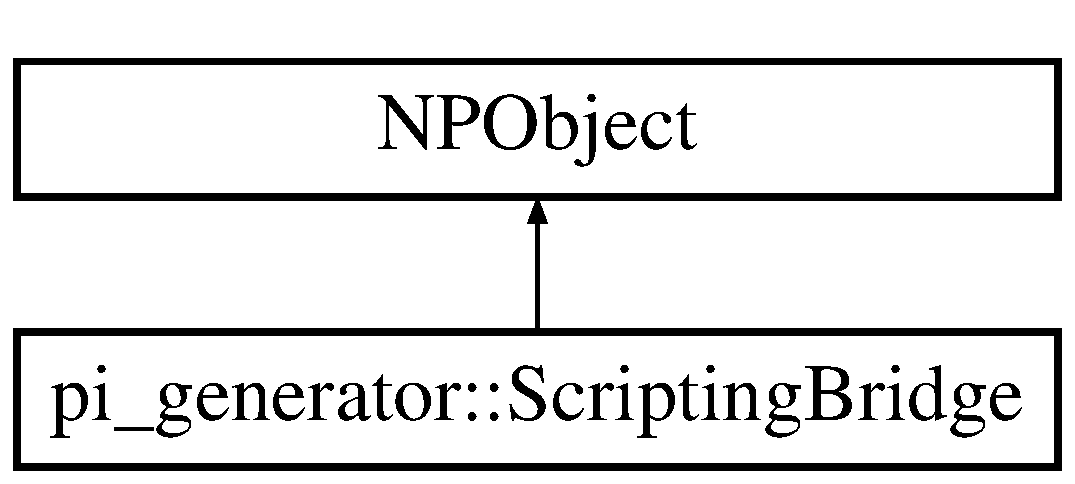
\includegraphics[height=2cm]{classpi__generator_1_1_scripting_bridge}
\end{center}
\end{figure}
\subsection*{Public Types}
\begin{DoxyCompactItemize}
\item 
typedef bool(ScriptingBridge::$\ast$ \hyperlink{classpi__generator_1_1_scripting_bridge_a48f5f7b0dfb3daabcdbfb3f7b667fd39}{Method} )(const \hyperlink{struct___n_p_variant}{NPVariant} $\ast$args, uint32\_\-t arg\_\-count, \hyperlink{struct___n_p_variant}{NPVariant} $\ast$result)
\item 
typedef bool(ScriptingBridge::$\ast$ \hyperlink{classpi__generator_1_1_scripting_bridge_abcd8cffa7f26f348e68cde316038245f}{Property} )(\hyperlink{struct___n_p_variant}{NPVariant} $\ast$result)
\end{DoxyCompactItemize}
\subsection*{Public Member Functions}
\begin{DoxyCompactItemize}
\item 
\hyperlink{classpi__generator_1_1_scripting_bridge_abcc778b6a4c482dff1ed271d7e776e42}{ScriptingBridge} (\hyperlink{struct___n_p_p}{NPP} npp)
\item 
virtual \hyperlink{classpi__generator_1_1_scripting_bridge_a605567080f40ddb9a6c2fa4ea9f2e876}{$\sim$ScriptingBridge} ()
\item 
virtual void \hyperlink{classpi__generator_1_1_scripting_bridge_a581ae88aa4acbefc30ae563452ab2fd5}{Invalidate} ()
\item 
virtual bool \hyperlink{classpi__generator_1_1_scripting_bridge_aaa99f91c8ced5df6fac0700516cdd058}{HasMethod} (\hyperlink{npruntime_8h_a3ce51391e08bd3e24128c342b1d055b9}{NPIdentifier} name)
\item 
virtual bool \hyperlink{classpi__generator_1_1_scripting_bridge_a3518781037308ae1d63bcdf5cc77a3de}{Invoke} (\hyperlink{npruntime_8h_a3ce51391e08bd3e24128c342b1d055b9}{NPIdentifier} name, const \hyperlink{struct___n_p_variant}{NPVariant} $\ast$args, uint32\_\-t arg\_\-count, \hyperlink{struct___n_p_variant}{NPVariant} $\ast$result)
\item 
virtual bool \hyperlink{classpi__generator_1_1_scripting_bridge_a0589fe559ec8b9297e37239233e238be}{InvokeDefault} (const \hyperlink{struct___n_p_variant}{NPVariant} $\ast$args, uint32\_\-t arg\_\-count, \hyperlink{struct___n_p_variant}{NPVariant} $\ast$result)
\item 
virtual bool \hyperlink{classpi__generator_1_1_scripting_bridge_a55f52d9e5e377367881e919db10b019f}{HasProperty} (\hyperlink{npruntime_8h_a3ce51391e08bd3e24128c342b1d055b9}{NPIdentifier} name)
\item 
virtual bool \hyperlink{classpi__generator_1_1_scripting_bridge_ab97693ce171c216783e79debb3b192cc}{GetProperty} (\hyperlink{npruntime_8h_a3ce51391e08bd3e24128c342b1d055b9}{NPIdentifier} name, \hyperlink{struct___n_p_variant}{NPVariant} $\ast$result)
\item 
virtual bool \hyperlink{classpi__generator_1_1_scripting_bridge_aa87ffdeb58a36a1e352814132d4a020a}{SetProperty} (\hyperlink{npruntime_8h_a3ce51391e08bd3e24128c342b1d055b9}{NPIdentifier} name, const \hyperlink{struct___n_p_variant}{NPVariant} $\ast$value)
\item 
virtual bool \hyperlink{classpi__generator_1_1_scripting_bridge_ab1a46993e1a36b9857d48776f7085aa2}{RemoveProperty} (\hyperlink{npruntime_8h_a3ce51391e08bd3e24128c342b1d055b9}{NPIdentifier} name)
\item 
bool \hyperlink{classpi__generator_1_1_scripting_bridge_afcd2c9c3e990cae2d713e8bb5d84048d}{Paint} (const \hyperlink{struct___n_p_variant}{NPVariant} $\ast$args, uint32\_\-t arg\_\-count, \hyperlink{struct___n_p_variant}{NPVariant} $\ast$result)
\end{DoxyCompactItemize}
\subsection*{Static Public Member Functions}
\begin{DoxyCompactItemize}
\item 
static bool \hyperlink{classpi__generator_1_1_scripting_bridge_a76184c7bc22d728d207e275b5f980d67}{InitializeIdentifiers} ()
\end{DoxyCompactItemize}
\subsection*{Static Public Attributes}
\begin{DoxyCompactItemize}
\item 
static \hyperlink{struct_n_p_class}{NPClass} \hyperlink{classpi__generator_1_1_scripting_bridge_a1756e8dff7625cda7697f3e9725ede25}{np\_\-class}
\end{DoxyCompactItemize}


\subsection{Detailed Description}


Definition at line 23 of file scripting\_\-bridge.h.



\subsection{Member Typedef Documentation}
\hypertarget{classpi__generator_1_1_scripting_bridge_a48f5f7b0dfb3daabcdbfb3f7b667fd39}{
\index{pi\_\-generator::ScriptingBridge@{pi\_\-generator::ScriptingBridge}!Method@{Method}}
\index{Method@{Method}!pi_generator::ScriptingBridge@{pi\_\-generator::ScriptingBridge}}
\subsubsection[{Method}]{\setlength{\rightskip}{0pt plus 5cm}typedef bool(ScriptingBridge::$\ast$ {\bf pi\_\-generator::ScriptingBridge::Method})(const {\bf NPVariant} $\ast$args, uint32\_\-t arg\_\-count, {\bf NPVariant} $\ast$result)}}
\label{classpi__generator_1_1_scripting_bridge_a48f5f7b0dfb3daabcdbfb3f7b667fd39}


Definition at line 25 of file scripting\_\-bridge.h.

\hypertarget{classpi__generator_1_1_scripting_bridge_abcd8cffa7f26f348e68cde316038245f}{
\index{pi\_\-generator::ScriptingBridge@{pi\_\-generator::ScriptingBridge}!Property@{Property}}
\index{Property@{Property}!pi_generator::ScriptingBridge@{pi\_\-generator::ScriptingBridge}}
\subsubsection[{Property}]{\setlength{\rightskip}{0pt plus 5cm}typedef bool(ScriptingBridge::$\ast$ {\bf pi\_\-generator::ScriptingBridge::Property})({\bf NPVariant} $\ast$result)}}
\label{classpi__generator_1_1_scripting_bridge_abcd8cffa7f26f348e68cde316038245f}


Definition at line 28 of file scripting\_\-bridge.h.



\subsection{Constructor \& Destructor Documentation}
\hypertarget{classpi__generator_1_1_scripting_bridge_abcc778b6a4c482dff1ed271d7e776e42}{
\index{pi\_\-generator::ScriptingBridge@{pi\_\-generator::ScriptingBridge}!ScriptingBridge@{ScriptingBridge}}
\index{ScriptingBridge@{ScriptingBridge}!pi_generator::ScriptingBridge@{pi\_\-generator::ScriptingBridge}}
\subsubsection[{ScriptingBridge}]{\setlength{\rightskip}{0pt plus 5cm}pi\_\-generator::ScriptingBridge::ScriptingBridge ({\bf NPP} {\em npp})\hspace{0.3cm}{\ttfamily  \mbox{[}inline, explicit\mbox{]}}}}
\label{classpi__generator_1_1_scripting_bridge_abcc778b6a4c482dff1ed271d7e776e42}


Definition at line 30 of file scripting\_\-bridge.h.

\hypertarget{classpi__generator_1_1_scripting_bridge_a605567080f40ddb9a6c2fa4ea9f2e876}{
\index{pi\_\-generator::ScriptingBridge@{pi\_\-generator::ScriptingBridge}!$\sim$ScriptingBridge@{$\sim$ScriptingBridge}}
\index{$\sim$ScriptingBridge@{$\sim$ScriptingBridge}!pi_generator::ScriptingBridge@{pi\_\-generator::ScriptingBridge}}
\subsubsection[{$\sim$ScriptingBridge}]{\setlength{\rightskip}{0pt plus 5cm}pi\_\-generator::ScriptingBridge::$\sim$ScriptingBridge ()\hspace{0.3cm}{\ttfamily  \mbox{[}virtual\mbox{]}}}}
\label{classpi__generator_1_1_scripting_bridge_a605567080f40ddb9a6c2fa4ea9f2e876}


Definition at line 43 of file scripting\_\-bridge.cc.



\subsection{Member Function Documentation}
\hypertarget{classpi__generator_1_1_scripting_bridge_ab97693ce171c216783e79debb3b192cc}{
\index{pi\_\-generator::ScriptingBridge@{pi\_\-generator::ScriptingBridge}!GetProperty@{GetProperty}}
\index{GetProperty@{GetProperty}!pi_generator::ScriptingBridge@{pi\_\-generator::ScriptingBridge}}
\subsubsection[{GetProperty}]{\setlength{\rightskip}{0pt plus 5cm}bool pi\_\-generator::ScriptingBridge::GetProperty ({\bf NPIdentifier} {\em name}, \/  {\bf NPVariant} $\ast$ {\em result})\hspace{0.3cm}{\ttfamily  \mbox{[}virtual\mbox{]}}}}
\label{classpi__generator_1_1_scripting_bridge_ab97693ce171c216783e79debb3b192cc}


Definition at line 64 of file scripting\_\-bridge.cc.

\hypertarget{classpi__generator_1_1_scripting_bridge_aaa99f91c8ced5df6fac0700516cdd058}{
\index{pi\_\-generator::ScriptingBridge@{pi\_\-generator::ScriptingBridge}!HasMethod@{HasMethod}}
\index{HasMethod@{HasMethod}!pi_generator::ScriptingBridge@{pi\_\-generator::ScriptingBridge}}
\subsubsection[{HasMethod}]{\setlength{\rightskip}{0pt plus 5cm}bool pi\_\-generator::ScriptingBridge::HasMethod ({\bf NPIdentifier} {\em name})\hspace{0.3cm}{\ttfamily  \mbox{[}virtual\mbox{]}}}}
\label{classpi__generator_1_1_scripting_bridge_aaa99f91c8ced5df6fac0700516cdd058}


Definition at line 48 of file scripting\_\-bridge.cc.

\hypertarget{classpi__generator_1_1_scripting_bridge_a55f52d9e5e377367881e919db10b019f}{
\index{pi\_\-generator::ScriptingBridge@{pi\_\-generator::ScriptingBridge}!HasProperty@{HasProperty}}
\index{HasProperty@{HasProperty}!pi_generator::ScriptingBridge@{pi\_\-generator::ScriptingBridge}}
\subsubsection[{HasProperty}]{\setlength{\rightskip}{0pt plus 5cm}bool pi\_\-generator::ScriptingBridge::HasProperty ({\bf NPIdentifier} {\em name})\hspace{0.3cm}{\ttfamily  \mbox{[}virtual\mbox{]}}}}
\label{classpi__generator_1_1_scripting_bridge_a55f52d9e5e377367881e919db10b019f}


Definition at line 56 of file scripting\_\-bridge.cc.

\hypertarget{classpi__generator_1_1_scripting_bridge_a76184c7bc22d728d207e275b5f980d67}{
\index{pi\_\-generator::ScriptingBridge@{pi\_\-generator::ScriptingBridge}!InitializeIdentifiers@{InitializeIdentifiers}}
\index{InitializeIdentifiers@{InitializeIdentifiers}!pi_generator::ScriptingBridge@{pi\_\-generator::ScriptingBridge}}
\subsubsection[{InitializeIdentifiers}]{\setlength{\rightskip}{0pt plus 5cm}bool pi\_\-generator::ScriptingBridge::InitializeIdentifiers ()\hspace{0.3cm}{\ttfamily  \mbox{[}static\mbox{]}}}}
\label{classpi__generator_1_1_scripting_bridge_a76184c7bc22d728d207e275b5f980d67}


Definition at line 22 of file scripting\_\-bridge.cc.

\hypertarget{classpi__generator_1_1_scripting_bridge_a581ae88aa4acbefc30ae563452ab2fd5}{
\index{pi\_\-generator::ScriptingBridge@{pi\_\-generator::ScriptingBridge}!Invalidate@{Invalidate}}
\index{Invalidate@{Invalidate}!pi_generator::ScriptingBridge@{pi\_\-generator::ScriptingBridge}}
\subsubsection[{Invalidate}]{\setlength{\rightskip}{0pt plus 5cm}void pi\_\-generator::ScriptingBridge::Invalidate ()\hspace{0.3cm}{\ttfamily  \mbox{[}virtual\mbox{]}}}}
\label{classpi__generator_1_1_scripting_bridge_a581ae88aa4acbefc30ae563452ab2fd5}


Definition at line 110 of file scripting\_\-bridge.cc.

\hypertarget{classpi__generator_1_1_scripting_bridge_a3518781037308ae1d63bcdf5cc77a3de}{
\index{pi\_\-generator::ScriptingBridge@{pi\_\-generator::ScriptingBridge}!Invoke@{Invoke}}
\index{Invoke@{Invoke}!pi_generator::ScriptingBridge@{pi\_\-generator::ScriptingBridge}}
\subsubsection[{Invoke}]{\setlength{\rightskip}{0pt plus 5cm}bool pi\_\-generator::ScriptingBridge::Invoke ({\bf NPIdentifier} {\em name}, \/  const {\bf NPVariant} $\ast$ {\em args}, \/  uint32\_\-t {\em arg\_\-count}, \/  {\bf NPVariant} $\ast$ {\em result})\hspace{0.3cm}{\ttfamily  \mbox{[}virtual\mbox{]}}}}
\label{classpi__generator_1_1_scripting_bridge_a3518781037308ae1d63bcdf5cc77a3de}


Definition at line 97 of file scripting\_\-bridge.cc.

\hypertarget{classpi__generator_1_1_scripting_bridge_a0589fe559ec8b9297e37239233e238be}{
\index{pi\_\-generator::ScriptingBridge@{pi\_\-generator::ScriptingBridge}!InvokeDefault@{InvokeDefault}}
\index{InvokeDefault@{InvokeDefault}!pi_generator::ScriptingBridge@{pi\_\-generator::ScriptingBridge}}
\subsubsection[{InvokeDefault}]{\setlength{\rightskip}{0pt plus 5cm}bool pi\_\-generator::ScriptingBridge::InvokeDefault (const {\bf NPVariant} $\ast$ {\em args}, \/  uint32\_\-t {\em arg\_\-count}, \/  {\bf NPVariant} $\ast$ {\em result})\hspace{0.3cm}{\ttfamily  \mbox{[}virtual\mbox{]}}}}
\label{classpi__generator_1_1_scripting_bridge_a0589fe559ec8b9297e37239233e238be}


Definition at line 89 of file scripting\_\-bridge.cc.

\hypertarget{classpi__generator_1_1_scripting_bridge_afcd2c9c3e990cae2d713e8bb5d84048d}{
\index{pi\_\-generator::ScriptingBridge@{pi\_\-generator::ScriptingBridge}!Paint@{Paint}}
\index{Paint@{Paint}!pi_generator::ScriptingBridge@{pi\_\-generator::ScriptingBridge}}
\subsubsection[{Paint}]{\setlength{\rightskip}{0pt plus 5cm}bool pi\_\-generator::ScriptingBridge::Paint (const {\bf NPVariant} $\ast$ {\em args}, \/  uint32\_\-t {\em arg\_\-count}, \/  {\bf NPVariant} $\ast$ {\em result})}}
\label{classpi__generator_1_1_scripting_bridge_afcd2c9c3e990cae2d713e8bb5d84048d}


Definition at line 114 of file scripting\_\-bridge.cc.

\hypertarget{classpi__generator_1_1_scripting_bridge_ab1a46993e1a36b9857d48776f7085aa2}{
\index{pi\_\-generator::ScriptingBridge@{pi\_\-generator::ScriptingBridge}!RemoveProperty@{RemoveProperty}}
\index{RemoveProperty@{RemoveProperty}!pi_generator::ScriptingBridge@{pi\_\-generator::ScriptingBridge}}
\subsubsection[{RemoveProperty}]{\setlength{\rightskip}{0pt plus 5cm}bool pi\_\-generator::ScriptingBridge::RemoveProperty ({\bf NPIdentifier} {\em name})\hspace{0.3cm}{\ttfamily  \mbox{[}virtual\mbox{]}}}}
\label{classpi__generator_1_1_scripting_bridge_ab1a46993e1a36b9857d48776f7085aa2}


Definition at line 83 of file scripting\_\-bridge.cc.

\hypertarget{classpi__generator_1_1_scripting_bridge_aa87ffdeb58a36a1e352814132d4a020a}{
\index{pi\_\-generator::ScriptingBridge@{pi\_\-generator::ScriptingBridge}!SetProperty@{SetProperty}}
\index{SetProperty@{SetProperty}!pi_generator::ScriptingBridge@{pi\_\-generator::ScriptingBridge}}
\subsubsection[{SetProperty}]{\setlength{\rightskip}{0pt plus 5cm}bool pi\_\-generator::ScriptingBridge::SetProperty ({\bf NPIdentifier} {\em name}, \/  const {\bf NPVariant} $\ast$ {\em value})\hspace{0.3cm}{\ttfamily  \mbox{[}virtual\mbox{]}}}}
\label{classpi__generator_1_1_scripting_bridge_aa87ffdeb58a36a1e352814132d4a020a}


Definition at line 77 of file scripting\_\-bridge.cc.



\subsection{Member Data Documentation}
\hypertarget{classpi__generator_1_1_scripting_bridge_a1756e8dff7625cda7697f3e9725ede25}{
\index{pi\_\-generator::ScriptingBridge@{pi\_\-generator::ScriptingBridge}!np\_\-class@{np\_\-class}}
\index{np\_\-class@{np\_\-class}!pi_generator::ScriptingBridge@{pi\_\-generator::ScriptingBridge}}
\subsubsection[{np\_\-class}]{\setlength{\rightskip}{0pt plus 5cm}{\bf NPClass} {\bf pi\_\-generator::ScriptingBridge::np\_\-class}\hspace{0.3cm}{\ttfamily  \mbox{[}static\mbox{]}}}}
\label{classpi__generator_1_1_scripting_bridge_a1756e8dff7625cda7697f3e9725ede25}
{\bfseries Initial value:}
\begin{DoxyCode}
 {
  NP_CLASS_STRUCT_VERSION,
  pi_generator::Allocate,
  pi_generator::Deallocate,
  pi_generator::Invalidate,
  pi_generator::HasMethod,
  pi_generator::Invoke,
  pi_generator::InvokeDefault,
  pi_generator::HasProperty,
  pi_generator::GetProperty,
  pi_generator::SetProperty,
  pi_generator::RemoveProperty
}
\end{DoxyCode}


Definition at line 51 of file scripting\_\-bridge.h.



The documentation for this class was generated from the following files:\begin{DoxyCompactItemize}
\item 
/home/derek/dev/cell-\/grid-\/game/nacl/crml/crml/test/pi\_\-generator/\hyperlink{test_2pi__generator_2scripting__bridge_8h}{scripting\_\-bridge.h}\item 
/home/derek/dev/cell-\/grid-\/game/nacl/crml/crml/core/\hyperlink{core_2scripting__bridge_8cc}{scripting\_\-bridge.cc}\item 
/home/derek/dev/cell-\/grid-\/game/nacl/crml/crml/test/pi\_\-generator/\hyperlink{test_2pi__generator_2scripting__bridge_8cc}{scripting\_\-bridge.cc}\end{DoxyCompactItemize}

\hypertarget{struct_test_object}{
\section{TestObject Struct Reference}
\label{struct_test_object}\index{TestObject@{TestObject}}
}


{\ttfamily \#include $<$test\_\-object.h$>$}

\subsection*{Public Attributes}
\begin{DoxyCompactItemize}
\item 
NPObject \hyperlink{struct_test_object_a23d7a50afe1b29f85b5d663cbfc763b2}{header}
\item 
NPObject $\ast$ \hyperlink{struct_test_object_a375c492938a3abf12d768b8578549861}{test\_\-object}
\end{DoxyCompactItemize}


\subsection{Detailed Description}


Definition at line 32 of file test\_\-object.h.



\subsection{Member Data Documentation}
\hypertarget{struct_test_object_a23d7a50afe1b29f85b5d663cbfc763b2}{
\index{TestObject@{TestObject}!header@{header}}
\index{header@{header}!TestObject@{TestObject}}
\subsubsection[{header}]{\setlength{\rightskip}{0pt plus 5cm}NPObject {\bf TestObject::header}}}
\label{struct_test_object_a23d7a50afe1b29f85b5d663cbfc763b2}


Definition at line 33 of file test\_\-object.h.

\hypertarget{struct_test_object_a375c492938a3abf12d768b8578549861}{
\index{TestObject@{TestObject}!test\_\-object@{test\_\-object}}
\index{test\_\-object@{test\_\-object}!TestObject@{TestObject}}
\subsubsection[{test\_\-object}]{\setlength{\rightskip}{0pt plus 5cm}NPObject $\ast$ {\bf TestObject::test\_\-object}}}
\label{struct_test_object_a375c492938a3abf12d768b8578549861}


Definition at line 34 of file test\_\-object.h.



The documentation for this struct was generated from the following files:\begin{DoxyCompactItemize}
\item 
/home/derek/dev/cell-\/grid-\/game/nacl/crml/crml/sys/\hyperlink{sys_2test__object_8h}{test\_\-object.h}\item 
/home/derek/dev/cell-\/grid-\/game/nacl/crml/crml/test/\hyperlink{test_2test__object_8h}{test\_\-object.h}\end{DoxyCompactItemize}

\hypertarget{classtumbler_1_1_tumbler}{
\section{tumbler::Tumbler Class Reference}
\label{classtumbler_1_1_tumbler}\index{tumbler::Tumbler@{tumbler::Tumbler}}
}


{\ttfamily \#include $<$tumbler.h$>$}

\subsection*{Public Member Functions}
\begin{DoxyCompactItemize}
\item 
\hyperlink{classtumbler_1_1_tumbler_a4f5dd0baa068ccb8214b0e477f7cd94b}{Tumbler} (NPP npp)
\item 
\hyperlink{classtumbler_1_1_tumbler_a80349e180aa825c15d63bada00c6e9a8}{$\sim$Tumbler} ()
\item 
NPObject $\ast$ \hyperlink{classtumbler_1_1_tumbler_ad438453c62d1edcbdd5cb39a38143a0b}{GetScriptableObject} ()
\item 
NPError \hyperlink{classtumbler_1_1_tumbler_a6aba2f3cfa10be35c0a789924343b1b0}{SetWindow} (const NPWindow \&window)
\item 
void \hyperlink{classtumbler_1_1_tumbler_ab721f5f95ce020ce6680033771ed4577}{PostRedrawNotification} ()
\item 
bool \hyperlink{classtumbler_1_1_tumbler_a8da0b0b0e85708487c55f6ca5c999da1}{DrawSelf} ()
\item 
bool \hyperlink{classtumbler_1_1_tumbler_a5e01d6cde9baab4e5c2aa4b834733bf2}{GetCameraOrientation} (float $\ast$orientation) const 
\item 
bool \hyperlink{classtumbler_1_1_tumbler_a2657d32f15492fc56406d1750172ca8c}{SetCameraOrientation} (const float $\ast$orientation)
\end{DoxyCompactItemize}


\subsection{Detailed Description}


Definition at line 38 of file tumbler.h.



\subsection{Constructor \& Destructor Documentation}
\hypertarget{classtumbler_1_1_tumbler_a4f5dd0baa068ccb8214b0e477f7cd94b}{
\index{tumbler::Tumbler@{tumbler::Tumbler}!Tumbler@{Tumbler}}
\index{Tumbler@{Tumbler}!tumbler::Tumbler@{tumbler::Tumbler}}
\subsubsection[{Tumbler}]{\setlength{\rightskip}{0pt plus 5cm}tumbler::Tumbler::Tumbler (NPP {\em npp})\hspace{0.3cm}{\ttfamily  \mbox{[}explicit\mbox{]}}}}
\label{classtumbler_1_1_tumbler_a4f5dd0baa068ccb8214b0e477f7cd94b}


Definition at line 38 of file tumbler.cc.

\hypertarget{classtumbler_1_1_tumbler_a80349e180aa825c15d63bada00c6e9a8}{
\index{tumbler::Tumbler@{tumbler::Tumbler}!$\sim$Tumbler@{$\sim$Tumbler}}
\index{$\sim$Tumbler@{$\sim$Tumbler}!tumbler::Tumbler@{tumbler::Tumbler}}
\subsubsection[{$\sim$Tumbler}]{\setlength{\rightskip}{0pt plus 5cm}tumbler::Tumbler::$\sim$Tumbler ()}}
\label{classtumbler_1_1_tumbler_a80349e180aa825c15d63bada00c6e9a8}


Definition at line 48 of file tumbler.cc.



\subsection{Member Function Documentation}
\hypertarget{classtumbler_1_1_tumbler_a8da0b0b0e85708487c55f6ca5c999da1}{
\index{tumbler::Tumbler@{tumbler::Tumbler}!DrawSelf@{DrawSelf}}
\index{DrawSelf@{DrawSelf}!tumbler::Tumbler@{tumbler::Tumbler}}
\subsubsection[{DrawSelf}]{\setlength{\rightskip}{0pt plus 5cm}bool tumbler::Tumbler::DrawSelf ()}}
\label{classtumbler_1_1_tumbler_a8da0b0b0e85708487c55f6ca5c999da1}


Definition at line 90 of file tumbler.cc.

\hypertarget{classtumbler_1_1_tumbler_a5e01d6cde9baab4e5c2aa4b834733bf2}{
\index{tumbler::Tumbler@{tumbler::Tumbler}!GetCameraOrientation@{GetCameraOrientation}}
\index{GetCameraOrientation@{GetCameraOrientation}!tumbler::Tumbler@{tumbler::Tumbler}}
\subsubsection[{GetCameraOrientation}]{\setlength{\rightskip}{0pt plus 5cm}bool tumbler::Tumbler::GetCameraOrientation (float $\ast$ {\em orientation}) const}}
\label{classtumbler_1_1_tumbler_a5e01d6cde9baab4e5c2aa4b834733bf2}


Definition at line 109 of file tumbler.cc.

\hypertarget{classtumbler_1_1_tumbler_ad438453c62d1edcbdd5cb39a38143a0b}{
\index{tumbler::Tumbler@{tumbler::Tumbler}!GetScriptableObject@{GetScriptableObject}}
\index{GetScriptableObject@{GetScriptableObject}!tumbler::Tumbler@{tumbler::Tumbler}}
\subsubsection[{GetScriptableObject}]{\setlength{\rightskip}{0pt plus 5cm}NPObject $\ast$ tumbler::Tumbler::GetScriptableObject ()}}
\label{classtumbler_1_1_tumbler_ad438453c62d1edcbdd5cb39a38143a0b}


Definition at line 60 of file tumbler.cc.

\hypertarget{classtumbler_1_1_tumbler_ab721f5f95ce020ce6680033771ed4577}{
\index{tumbler::Tumbler@{tumbler::Tumbler}!PostRedrawNotification@{PostRedrawNotification}}
\index{PostRedrawNotification@{PostRedrawNotification}!tumbler::Tumbler@{tumbler::Tumbler}}
\subsubsection[{PostRedrawNotification}]{\setlength{\rightskip}{0pt plus 5cm}void tumbler::Tumbler::PostRedrawNotification ()}}
\label{classtumbler_1_1_tumbler_ab721f5f95ce020ce6680033771ed4577}


Definition at line 86 of file tumbler.cc.

\hypertarget{classtumbler_1_1_tumbler_a2657d32f15492fc56406d1750172ca8c}{
\index{tumbler::Tumbler@{tumbler::Tumbler}!SetCameraOrientation@{SetCameraOrientation}}
\index{SetCameraOrientation@{SetCameraOrientation}!tumbler::Tumbler@{tumbler::Tumbler}}
\subsubsection[{SetCameraOrientation}]{\setlength{\rightskip}{0pt plus 5cm}bool tumbler::Tumbler::SetCameraOrientation (const float $\ast$ {\em orientation})}}
\label{classtumbler_1_1_tumbler_a2657d32f15492fc56406d1750172ca8c}


Definition at line 117 of file tumbler.cc.

\hypertarget{classtumbler_1_1_tumbler_a6aba2f3cfa10be35c0a789924343b1b0}{
\index{tumbler::Tumbler@{tumbler::Tumbler}!SetWindow@{SetWindow}}
\index{SetWindow@{SetWindow}!tumbler::Tumbler@{tumbler::Tumbler}}
\subsubsection[{SetWindow}]{\setlength{\rightskip}{0pt plus 5cm}NPError tumbler::Tumbler::SetWindow (const NPWindow \& {\em window})}}
\label{classtumbler_1_1_tumbler_a6aba2f3cfa10be35c0a789924343b1b0}


Definition at line 71 of file tumbler.cc.



The documentation for this class was generated from the following files:\begin{DoxyCompactItemize}
\item 
/home/derek/dev/crml/crml/lib/tumbler/\hyperlink{tumbler_8h}{tumbler.h}\item 
/home/derek/dev/crml/crml/lib/tumbler/\hyperlink{tumbler_8cc}{tumbler.cc}\end{DoxyCompactItemize}

\hypertarget{structtumbler_1_1_tumbler_context3_d}{
\section{tumbler::TumblerContext3D Struct Reference}
\label{structtumbler_1_1_tumbler_context3_d}\index{tumbler::TumblerContext3D@{tumbler::TumblerContext3D}}
}


{\ttfamily \#include $<$tumbler.h$>$}

\subsection*{Public Attributes}
\begin{DoxyCompactItemize}
\item 
void $\ast$ \hyperlink{structtumbler_1_1_tumbler_context3_d_a1274a5b24b002c4e264bc7ee9298e85d}{user\_\-data\_\-}
\end{DoxyCompactItemize}


\subsection{Detailed Description}


Definition at line 34 of file tumbler.h.



\subsection{Member Data Documentation}
\hypertarget{structtumbler_1_1_tumbler_context3_d_a1274a5b24b002c4e264bc7ee9298e85d}{
\index{tumbler::TumblerContext3D@{tumbler::TumblerContext3D}!user\_\-data\_\-@{user\_\-data\_\-}}
\index{user\_\-data\_\-@{user\_\-data\_\-}!tumbler::TumblerContext3D@{tumbler::TumblerContext3D}}
\subsubsection[{user\_\-data\_\-}]{\setlength{\rightskip}{0pt plus 5cm}void$\ast$ {\bf tumbler::TumblerContext3D::user\_\-data\_\-}}}
\label{structtumbler_1_1_tumbler_context3_d_a1274a5b24b002c4e264bc7ee9298e85d}


Definition at line 35 of file tumbler.h.



The documentation for this struct was generated from the following file:\begin{DoxyCompactItemize}
\item 
/home/derek/dev/crml/crml/lib/tumbler/\hyperlink{tumbler_8h}{tumbler.h}\end{DoxyCompactItemize}

\chapter{File Documentation}
\hypertarget{basic__macros_8h}{
\section{/home/derek/dev/cell-\/grid-\/game/nacl/crml/crml/lib/tumbler/basic\_\-macros.h File Reference}
\label{basic__macros_8h}\index{/home/derek/dev/cell-\/grid-\/game/nacl/crml/crml/lib/tumbler/basic\_\-macros.h@{/home/derek/dev/cell-\/grid-\/game/nacl/crml/crml/lib/tumbler/basic\_\-macros.h}}
}
\subsection*{Defines}
\begin{DoxyCompactItemize}
\item 
\#define \hyperlink{basic__macros_8h_af8df3547bfde53a5acb93e2607b0034a}{DISALLOW\_\-COPY\_\-AND\_\-ASSIGN}(TypeName)
\item 
\#define \hyperlink{basic__macros_8h_acfd97435e2829938f396946b00559b71}{DISALLOW\_\-IMPLICIT\_\-CONSTRUCTORS}(TypeName)
\end{DoxyCompactItemize}


\subsection{Define Documentation}
\hypertarget{basic__macros_8h_af8df3547bfde53a5acb93e2607b0034a}{
\index{basic\_\-macros.h@{basic\_\-macros.h}!DISALLOW\_\-COPY\_\-AND\_\-ASSIGN@{DISALLOW\_\-COPY\_\-AND\_\-ASSIGN}}
\index{DISALLOW\_\-COPY\_\-AND\_\-ASSIGN@{DISALLOW\_\-COPY\_\-AND\_\-ASSIGN}!basic_macros.h@{basic\_\-macros.h}}
\subsubsection[{DISALLOW\_\-COPY\_\-AND\_\-ASSIGN}]{\setlength{\rightskip}{0pt plus 5cm}\#define DISALLOW\_\-COPY\_\-AND\_\-ASSIGN(TypeName)}}
\label{basic__macros_8h_af8df3547bfde53a5acb93e2607b0034a}
{\bfseries Value:}
\begin{DoxyCode}
TypeName(const TypeName&);               \
  void operator=(const TypeName&)
\end{DoxyCode}


Definition at line 10 of file basic\_\-macros.h.

\hypertarget{basic__macros_8h_acfd97435e2829938f396946b00559b71}{
\index{basic\_\-macros.h@{basic\_\-macros.h}!DISALLOW\_\-IMPLICIT\_\-CONSTRUCTORS@{DISALLOW\_\-IMPLICIT\_\-CONSTRUCTORS}}
\index{DISALLOW\_\-IMPLICIT\_\-CONSTRUCTORS@{DISALLOW\_\-IMPLICIT\_\-CONSTRUCTORS}!basic_macros.h@{basic\_\-macros.h}}
\subsubsection[{DISALLOW\_\-IMPLICIT\_\-CONSTRUCTORS}]{\setlength{\rightskip}{0pt plus 5cm}\#define DISALLOW\_\-IMPLICIT\_\-CONSTRUCTORS(TypeName)}}
\label{basic__macros_8h_acfd97435e2829938f396946b00559b71}
{\bfseries Value:}
\begin{DoxyCode}
TypeName();                                    \
  DISALLOW_COPY_AND_ASSIGN(TypeName)
\end{DoxyCode}


Definition at line 20 of file basic\_\-macros.h.


\hypertarget{cube_8cc}{
\section{/home/derek/dev/cell-\/grid-\/game/nacl/crml/crml/lib/tumbler/cube.cc File Reference}
\label{cube_8cc}\index{/home/derek/dev/cell-\/grid-\/game/nacl/crml/crml/lib/tumbler/cube.cc@{/home/derek/dev/cell-\/grid-\/game/nacl/crml/crml/lib/tumbler/cube.cc}}
}
{\ttfamily \#include \char`\"{}examples/tumbler/cube.h\char`\"{}}\par
{\ttfamily \#include $<$algorithm$>$}\par
{\ttfamily \#include \char`\"{}examples/tumbler/shader\_\-util.h\char`\"{}}\par
{\ttfamily \#include \char`\"{}examples/tumbler/transforms.h\char`\"{}}\par
\subsection*{Namespaces}
\begin{DoxyCompactItemize}
\item 
namespace \hyperlink{namespacetumbler}{tumbler}
\end{DoxyCompactItemize}

\hypertarget{cube_8h}{
\section{/home/derek/dev/cell-\/grid-\/game/nacl/crml/crml/lib/tumbler/cube.h File Reference}
\label{cube_8h}\index{/home/derek/dev/cell-\/grid-\/game/nacl/crml/crml/lib/tumbler/cube.h@{/home/derek/dev/cell-\/grid-\/game/nacl/crml/crml/lib/tumbler/cube.h}}
}
{\ttfamily \#include $<$GLES2/gl2.h$>$}\par
{\ttfamily \#include \char`\"{}examples/tumbler/basic\_\-macros.h\char`\"{}}\par
\subsection*{Classes}
\begin{DoxyCompactItemize}
\item 
class \hyperlink{classtumbler_1_1_cube}{tumbler::Cube}
\end{DoxyCompactItemize}
\subsection*{Namespaces}
\begin{DoxyCompactItemize}
\item 
namespace \hyperlink{namespacetumbler}{tumbler}
\end{DoxyCompactItemize}

\hypertarget{lib_2tumbler_2npn__bridge_8cc}{
\section{/home/derek/dev/crml/crml/lib/tumbler/npn\_\-bridge.cc File Reference}
\label{lib_2tumbler_2npn__bridge_8cc}\index{/home/derek/dev/crml/crml/lib/tumbler/npn\_\-bridge.cc@{/home/derek/dev/crml/crml/lib/tumbler/npn\_\-bridge.cc}}
}
{\ttfamily \#include $<$assert.h$>$}\par
{\ttfamily \#include $<$nacl/npapi\_\-extensions.h$>$}\par
{\ttfamily \#include $<$nacl/npupp.h$>$}\par
\subsection*{Functions}
\begin{DoxyCompactItemize}
\item 
void \hyperlink{lib_2tumbler_2npn__bridge_8cc_a4084a1c4bd65fa38046b67c758bd6862}{InitializePepperExtensions} (NPP instance)
\item 
NPDevice $\ast$ \hyperlink{lib_2tumbler_2npn__bridge_8cc_af6ca8d586b1bc4be36e2a870354c019b}{NPN\_\-AcquireDevice} (NPP instance, NPDeviceID device)
\end{DoxyCompactItemize}


\subsection{Function Documentation}
\hypertarget{lib_2tumbler_2npn__bridge_8cc_a4084a1c4bd65fa38046b67c758bd6862}{
\index{lib/tumbler/npn\_\-bridge.cc@{lib/tumbler/npn\_\-bridge.cc}!InitializePepperExtensions@{InitializePepperExtensions}}
\index{InitializePepperExtensions@{InitializePepperExtensions}!lib/tumbler/npn_bridge.cc@{lib/tumbler/npn\_\-bridge.cc}}
\subsubsection[{InitializePepperExtensions}]{\setlength{\rightskip}{0pt plus 5cm}void InitializePepperExtensions (NPP {\em instance})}}
\label{lib_2tumbler_2npn__bridge_8cc_a4084a1c4bd65fa38046b67c758bd6862}


Definition at line 20 of file npn\_\-bridge.cc.

\hypertarget{lib_2tumbler_2npn__bridge_8cc_af6ca8d586b1bc4be36e2a870354c019b}{
\index{lib/tumbler/npn\_\-bridge.cc@{lib/tumbler/npn\_\-bridge.cc}!NPN\_\-AcquireDevice@{NPN\_\-AcquireDevice}}
\index{NPN\_\-AcquireDevice@{NPN\_\-AcquireDevice}!lib/tumbler/npn_bridge.cc@{lib/tumbler/npn\_\-bridge.cc}}
\subsubsection[{NPN\_\-AcquireDevice}]{\setlength{\rightskip}{0pt plus 5cm}NPDevice$\ast$ NPN\_\-AcquireDevice (NPP {\em instance}, \/  NPDeviceID {\em device})}}
\label{lib_2tumbler_2npn__bridge_8cc_af6ca8d586b1bc4be36e2a870354c019b}


Definition at line 31 of file npn\_\-bridge.cc.


\hypertarget{src_2core_2npn__bridge_8cc}{
\section{/home/derek/dev/crml/crml/src/core/npn\_\-bridge.cc File Reference}
\label{src_2core_2npn__bridge_8cc}\index{/home/derek/dev/crml/crml/src/core/npn\_\-bridge.cc@{/home/derek/dev/crml/crml/src/core/npn\_\-bridge.cc}}
}
{\ttfamily \#include $<$assert.h$>$}\par
{\ttfamily \#include $<$nacl/npapi\_\-extensions.h$>$}\par
{\ttfamily \#include $<$nacl/npupp.h$>$}\par
\subsection*{Functions}
\begin{DoxyCompactItemize}
\item 
void \hyperlink{src_2core_2npn__bridge_8cc_a4084a1c4bd65fa38046b67c758bd6862}{InitializePepperExtensions} (NPP instance)
\item 
NPDevice $\ast$ \hyperlink{src_2core_2npn__bridge_8cc_af6ca8d586b1bc4be36e2a870354c019b}{NPN\_\-AcquireDevice} (NPP instance, NPDeviceID device)
\end{DoxyCompactItemize}


\subsection{Function Documentation}
\hypertarget{src_2core_2npn__bridge_8cc_a4084a1c4bd65fa38046b67c758bd6862}{
\index{src/core/npn\_\-bridge.cc@{src/core/npn\_\-bridge.cc}!InitializePepperExtensions@{InitializePepperExtensions}}
\index{InitializePepperExtensions@{InitializePepperExtensions}!src/core/npn_bridge.cc@{src/core/npn\_\-bridge.cc}}
\subsubsection[{InitializePepperExtensions}]{\setlength{\rightskip}{0pt plus 5cm}void InitializePepperExtensions (NPP {\em instance})}}
\label{src_2core_2npn__bridge_8cc_a4084a1c4bd65fa38046b67c758bd6862}


Definition at line 20 of file npn\_\-bridge.cc.

\hypertarget{src_2core_2npn__bridge_8cc_af6ca8d586b1bc4be36e2a870354c019b}{
\index{src/core/npn\_\-bridge.cc@{src/core/npn\_\-bridge.cc}!NPN\_\-AcquireDevice@{NPN\_\-AcquireDevice}}
\index{NPN\_\-AcquireDevice@{NPN\_\-AcquireDevice}!src/core/npn_bridge.cc@{src/core/npn\_\-bridge.cc}}
\subsubsection[{NPN\_\-AcquireDevice}]{\setlength{\rightskip}{0pt plus 5cm}NPDevice$\ast$ NPN\_\-AcquireDevice (NPP {\em instance}, \/  NPDeviceID {\em device})}}
\label{src_2core_2npn__bridge_8cc_af6ca8d586b1bc4be36e2a870354c019b}


Definition at line 31 of file npn\_\-bridge.cc.


\hypertarget{test_2crml__hello__world_2npn__bridge_8cc}{
\section{/home/derek/dev/crml/crml/test/crml\_\-hello\_\-world/npn\_\-bridge.cc File Reference}
\label{test_2crml__hello__world_2npn__bridge_8cc}\index{/home/derek/dev/crml/crml/test/crml\_\-hello\_\-world/npn\_\-bridge.cc@{/home/derek/dev/crml/crml/test/crml\_\-hello\_\-world/npn\_\-bridge.cc}}
}
{\ttfamily \#include $<$assert.h$>$}\par
{\ttfamily \#include $<$nacl/npapi\_\-extensions.h$>$}\par
{\ttfamily \#include $<$nacl/npupp.h$>$}\par
\subsection*{Functions}
\begin{DoxyCompactItemize}
\item 
void \hyperlink{test_2crml__hello__world_2npn__bridge_8cc_a4084a1c4bd65fa38046b67c758bd6862}{InitializePepperExtensions} (NPP instance)
\item 
NPDevice $\ast$ \hyperlink{test_2crml__hello__world_2npn__bridge_8cc_af6ca8d586b1bc4be36e2a870354c019b}{NPN\_\-AcquireDevice} (NPP instance, NPDeviceID device)
\end{DoxyCompactItemize}


\subsection{Function Documentation}
\hypertarget{test_2crml__hello__world_2npn__bridge_8cc_a4084a1c4bd65fa38046b67c758bd6862}{
\index{test/crml\_\-hello\_\-world/npn\_\-bridge.cc@{test/crml\_\-hello\_\-world/npn\_\-bridge.cc}!InitializePepperExtensions@{InitializePepperExtensions}}
\index{InitializePepperExtensions@{InitializePepperExtensions}!test/crml_hello_world/npn_bridge.cc@{test/crml\_\-hello\_\-world/npn\_\-bridge.cc}}
\subsubsection[{InitializePepperExtensions}]{\setlength{\rightskip}{0pt plus 5cm}void InitializePepperExtensions (NPP {\em instance})}}
\label{test_2crml__hello__world_2npn__bridge_8cc_a4084a1c4bd65fa38046b67c758bd6862}


Definition at line 20 of file npn\_\-bridge.cc.

\hypertarget{test_2crml__hello__world_2npn__bridge_8cc_af6ca8d586b1bc4be36e2a870354c019b}{
\index{test/crml\_\-hello\_\-world/npn\_\-bridge.cc@{test/crml\_\-hello\_\-world/npn\_\-bridge.cc}!NPN\_\-AcquireDevice@{NPN\_\-AcquireDevice}}
\index{NPN\_\-AcquireDevice@{NPN\_\-AcquireDevice}!test/crml_hello_world/npn_bridge.cc@{test/crml\_\-hello\_\-world/npn\_\-bridge.cc}}
\subsubsection[{NPN\_\-AcquireDevice}]{\setlength{\rightskip}{0pt plus 5cm}NPDevice$\ast$ NPN\_\-AcquireDevice (NPP {\em instance}, \/  NPDeviceID {\em device})}}
\label{test_2crml__hello__world_2npn__bridge_8cc_af6ca8d586b1bc4be36e2a870354c019b}


Definition at line 31 of file npn\_\-bridge.cc.


\hypertarget{test_2crml__pi__generator_2npn__bridge_8cc}{
\section{/home/derek/dev/crml/crml/test/crml\_\-pi\_\-generator/npn\_\-bridge.cc File Reference}
\label{test_2crml__pi__generator_2npn__bridge_8cc}\index{/home/derek/dev/crml/crml/test/crml\_\-pi\_\-generator/npn\_\-bridge.cc@{/home/derek/dev/crml/crml/test/crml\_\-pi\_\-generator/npn\_\-bridge.cc}}
}
{\ttfamily \#include $<$assert.h$>$}\par
{\ttfamily \#include $<$nacl/npapi\_\-extensions.h$>$}\par
{\ttfamily \#include $<$nacl/npupp.h$>$}\par
\subsection*{Functions}
\begin{DoxyCompactItemize}
\item 
void \hyperlink{test_2crml__pi__generator_2npn__bridge_8cc_a4084a1c4bd65fa38046b67c758bd6862}{InitializePepperExtensions} (NPP instance)
\item 
NPDevice $\ast$ \hyperlink{test_2crml__pi__generator_2npn__bridge_8cc_af6ca8d586b1bc4be36e2a870354c019b}{NPN\_\-AcquireDevice} (NPP instance, NPDeviceID device)
\end{DoxyCompactItemize}


\subsection{Function Documentation}
\hypertarget{test_2crml__pi__generator_2npn__bridge_8cc_a4084a1c4bd65fa38046b67c758bd6862}{
\index{test/crml\_\-pi\_\-generator/npn\_\-bridge.cc@{test/crml\_\-pi\_\-generator/npn\_\-bridge.cc}!InitializePepperExtensions@{InitializePepperExtensions}}
\index{InitializePepperExtensions@{InitializePepperExtensions}!test/crml_pi_generator/npn_bridge.cc@{test/crml\_\-pi\_\-generator/npn\_\-bridge.cc}}
\subsubsection[{InitializePepperExtensions}]{\setlength{\rightskip}{0pt plus 5cm}void InitializePepperExtensions (NPP {\em instance})}}
\label{test_2crml__pi__generator_2npn__bridge_8cc_a4084a1c4bd65fa38046b67c758bd6862}


Definition at line 20 of file npn\_\-bridge.cc.

\hypertarget{test_2crml__pi__generator_2npn__bridge_8cc_af6ca8d586b1bc4be36e2a870354c019b}{
\index{test/crml\_\-pi\_\-generator/npn\_\-bridge.cc@{test/crml\_\-pi\_\-generator/npn\_\-bridge.cc}!NPN\_\-AcquireDevice@{NPN\_\-AcquireDevice}}
\index{NPN\_\-AcquireDevice@{NPN\_\-AcquireDevice}!test/crml_pi_generator/npn_bridge.cc@{test/crml\_\-pi\_\-generator/npn\_\-bridge.cc}}
\subsubsection[{NPN\_\-AcquireDevice}]{\setlength{\rightskip}{0pt plus 5cm}NPDevice$\ast$ NPN\_\-AcquireDevice (NPP {\em instance}, \/  NPDeviceID {\em device})}}
\label{test_2crml__pi__generator_2npn__bridge_8cc_af6ca8d586b1bc4be36e2a870354c019b}


Definition at line 31 of file npn\_\-bridge.cc.


\hypertarget{test_2pi__generator_2npn__bridge_8cc}{
\section{/home/derek/dev/cell-\/grid-\/game/nacl/crml/crml/test/pi\_\-generator/npn\_\-bridge.cc File Reference}
\label{test_2pi__generator_2npn__bridge_8cc}\index{/home/derek/dev/cell-\/grid-\/game/nacl/crml/crml/test/pi\_\-generator/npn\_\-bridge.cc@{/home/derek/dev/cell-\/grid-\/game/nacl/crml/crml/test/pi\_\-generator/npn\_\-bridge.cc}}
}
{\ttfamily \#include $<$assert.h$>$}\par
{\ttfamily \#include $<$nacl/npapi\_\-extensions.h$>$}\par
{\ttfamily \#include $<$nacl/npupp.h$>$}\par
\subsection*{Functions}
\begin{DoxyCompactItemize}
\item 
void \hyperlink{test_2pi__generator_2npn__bridge_8cc_a4084a1c4bd65fa38046b67c758bd6862}{InitializePepperExtensions} (\hyperlink{struct___n_p_p}{NPP} instance)
\item 
\hyperlink{struct_n_p_device}{NPDevice} $\ast$ \hyperlink{test_2pi__generator_2npn__bridge_8cc_af6ca8d586b1bc4be36e2a870354c019b}{NPN\_\-AcquireDevice} (\hyperlink{struct___n_p_p}{NPP} instance, \hyperlink{npapi__extensions_8h_af06c24765f895a9b7ac2af96d8db1e61}{NPDeviceID} device)
\end{DoxyCompactItemize}


\subsection{Function Documentation}
\hypertarget{test_2pi__generator_2npn__bridge_8cc_a4084a1c4bd65fa38046b67c758bd6862}{
\index{test/pi\_\-generator/npn\_\-bridge.cc@{test/pi\_\-generator/npn\_\-bridge.cc}!InitializePepperExtensions@{InitializePepperExtensions}}
\index{InitializePepperExtensions@{InitializePepperExtensions}!test/pi_generator/npn_bridge.cc@{test/pi\_\-generator/npn\_\-bridge.cc}}
\subsubsection[{InitializePepperExtensions}]{\setlength{\rightskip}{0pt plus 5cm}void InitializePepperExtensions ({\bf NPP} {\em instance})}}
\label{test_2pi__generator_2npn__bridge_8cc_a4084a1c4bd65fa38046b67c758bd6862}


Definition at line 20 of file npn\_\-bridge.cc.

\hypertarget{test_2pi__generator_2npn__bridge_8cc_af6ca8d586b1bc4be36e2a870354c019b}{
\index{test/pi\_\-generator/npn\_\-bridge.cc@{test/pi\_\-generator/npn\_\-bridge.cc}!NPN\_\-AcquireDevice@{NPN\_\-AcquireDevice}}
\index{NPN\_\-AcquireDevice@{NPN\_\-AcquireDevice}!test/pi_generator/npn_bridge.cc@{test/pi\_\-generator/npn\_\-bridge.cc}}
\subsubsection[{NPN\_\-AcquireDevice}]{\setlength{\rightskip}{0pt plus 5cm}{\bf NPDevice}$\ast$ NPN\_\-AcquireDevice ({\bf NPP} {\em instance}, \/  {\bf NPDeviceID} {\em device})}}
\label{test_2pi__generator_2npn__bridge_8cc_af6ca8d586b1bc4be36e2a870354c019b}


Definition at line 31 of file npn\_\-bridge.cc.


\hypertarget{lib_2tumbler_2npp__gate_8cc}{
\section{/home/derek/dev/cell-\/grid-\/game/nacl/crml/crml/lib/tumbler/npp\_\-gate.cc File Reference}
\label{lib_2tumbler_2npp__gate_8cc}\index{/home/derek/dev/cell-\/grid-\/game/nacl/crml/crml/lib/tumbler/npp\_\-gate.cc@{/home/derek/dev/cell-\/grid-\/game/nacl/crml/crml/lib/tumbler/npp\_\-gate.cc}}
}
{\ttfamily \#include $<$assert.h$>$}\par
{\ttfamily \#include $<$stdio.h$>$}\par
{\ttfamily \#include $<$string.h$>$}\par
{\ttfamily \#include $<$nacl/npupp.h$>$}\par
{\ttfamily \#include $<$new$>$}\par
{\ttfamily \#include \char`\"{}examples/tumbler/tumbler.h\char`\"{}}\par
\subsection*{Functions}
\begin{DoxyCompactItemize}
\item 
\hyperlink{npapi_8h_a56715bc92ac93f0447a05f852ce18828}{NPError} \hyperlink{lib_2tumbler_2npp__gate_8cc_a1549c7141eb65cb6eca02d3cba8f48d1}{NPP\_\-New} (\hyperlink{npapi_8h_a6ab16d9f607aeb576061783638ae2973}{NPMIMEType} mime\_\-type, \hyperlink{struct___n_p_p}{NPP} instance, uint16\_\-t mode, int16\_\-t argc, char $\ast$argn\mbox{[}$\,$\mbox{]}, char $\ast$argv\mbox{[}$\,$\mbox{]}, \hyperlink{struct___n_p_saved_data}{NPSavedData} $\ast$saved)
\item 
\hyperlink{npapi_8h_a56715bc92ac93f0447a05f852ce18828}{NPError} \hyperlink{lib_2tumbler_2npp__gate_8cc_a13cdb3ad1ae5ab428bd418ce64af269f}{NPP\_\-Destroy} (\hyperlink{struct___n_p_p}{NPP} instance, \hyperlink{struct___n_p_saved_data}{NPSavedData} $\ast$$\ast$save)
\item 
NPObject $\ast$ \hyperlink{lib_2tumbler_2npp__gate_8cc_ad6b92f15011abb6dde0ae16e86f46ed7}{NPP\_\-GetScriptableInstance} (\hyperlink{struct___n_p_p}{NPP} instance)
\item 
\hyperlink{npapi_8h_a56715bc92ac93f0447a05f852ce18828}{NPError} \hyperlink{lib_2tumbler_2npp__gate_8cc_aae56cbb0b1b9e955b67b98f8178fbeef}{NPP\_\-GetValue} (\hyperlink{struct___n_p_p}{NPP} instance, \hyperlink{npapi_8h_a1b56dde896277605195e0fad69cbca7d}{NPPVariable} variable, void $\ast$value)
\item 
int16\_\-t \hyperlink{lib_2tumbler_2npp__gate_8cc_afc9809fb9d0ee0ed5666723b2db78161}{NPP\_\-HandleEvent} (\hyperlink{struct___n_p_p}{NPP} instance, void $\ast$event)
\item 
\hyperlink{npapi_8h_a56715bc92ac93f0447a05f852ce18828}{NPError} \hyperlink{lib_2tumbler_2npp__gate_8cc_a352d8aac09e759465185ddd4eeea9df9}{NPP\_\-SetWindow} (\hyperlink{struct___n_p_p}{NPP} instance, \hyperlink{struct___n_p_window}{NPWindow} $\ast$window)
\item 
\hyperlink{npapi_8h_a56715bc92ac93f0447a05f852ce18828}{NPError} \hyperlink{lib_2tumbler_2npp__gate_8cc_a2e202c35d113ebeb05eb2175fc8d97cb}{InitializePluginFunctions} (NPPluginFuncs $\ast$plugin\_\-funcs)
\end{DoxyCompactItemize}


\subsection{Function Documentation}
\hypertarget{lib_2tumbler_2npp__gate_8cc_a2e202c35d113ebeb05eb2175fc8d97cb}{
\index{lib/tumbler/npp\_\-gate.cc@{lib/tumbler/npp\_\-gate.cc}!InitializePluginFunctions@{InitializePluginFunctions}}
\index{InitializePluginFunctions@{InitializePluginFunctions}!lib/tumbler/npp_gate.cc@{lib/tumbler/npp\_\-gate.cc}}
\subsubsection[{InitializePluginFunctions}]{\setlength{\rightskip}{0pt plus 5cm}{\bf NPError} InitializePluginFunctions (NPPluginFuncs $\ast$ {\em plugin\_\-funcs})}}
\label{lib_2tumbler_2npp__gate_8cc_a2e202c35d113ebeb05eb2175fc8d97cb}


Definition at line 133 of file npp\_\-gate.cc.

\hypertarget{lib_2tumbler_2npp__gate_8cc_a13cdb3ad1ae5ab428bd418ce64af269f}{
\index{lib/tumbler/npp\_\-gate.cc@{lib/tumbler/npp\_\-gate.cc}!NPP\_\-Destroy@{NPP\_\-Destroy}}
\index{NPP\_\-Destroy@{NPP\_\-Destroy}!lib/tumbler/npp_gate.cc@{lib/tumbler/npp\_\-gate.cc}}
\subsubsection[{NPP\_\-Destroy}]{\setlength{\rightskip}{0pt plus 5cm}{\bf NPError} NPP\_\-Destroy ({\bf NPP} {\em instance}, \/  {\bf NPSavedData} $\ast$$\ast$ {\em save})}}
\label{lib_2tumbler_2npp__gate_8cc_a13cdb3ad1ae5ab428bd418ce64af269f}


Definition at line 55 of file npp\_\-gate.cc.

\hypertarget{lib_2tumbler_2npp__gate_8cc_ad6b92f15011abb6dde0ae16e86f46ed7}{
\index{lib/tumbler/npp\_\-gate.cc@{lib/tumbler/npp\_\-gate.cc}!NPP\_\-GetScriptableInstance@{NPP\_\-GetScriptableInstance}}
\index{NPP\_\-GetScriptableInstance@{NPP\_\-GetScriptableInstance}!lib/tumbler/npp_gate.cc@{lib/tumbler/npp\_\-gate.cc}}
\subsubsection[{NPP\_\-GetScriptableInstance}]{\setlength{\rightskip}{0pt plus 5cm}NPObject$\ast$ NPP\_\-GetScriptableInstance ({\bf NPP} {\em instance})}}
\label{lib_2tumbler_2npp__gate_8cc_ad6b92f15011abb6dde0ae16e86f46ed7}


Definition at line 74 of file npp\_\-gate.cc.

\hypertarget{lib_2tumbler_2npp__gate_8cc_aae56cbb0b1b9e955b67b98f8178fbeef}{
\index{lib/tumbler/npp\_\-gate.cc@{lib/tumbler/npp\_\-gate.cc}!NPP\_\-GetValue@{NPP\_\-GetValue}}
\index{NPP\_\-GetValue@{NPP\_\-GetValue}!lib/tumbler/npp_gate.cc@{lib/tumbler/npp\_\-gate.cc}}
\subsubsection[{NPP\_\-GetValue}]{\setlength{\rightskip}{0pt plus 5cm}{\bf NPError} NPP\_\-GetValue ({\bf NPP} {\em instance}, \/  {\bf NPPVariable} {\em variable}, \/  void $\ast$ {\em value})}}
\label{lib_2tumbler_2npp__gate_8cc_aae56cbb0b1b9e955b67b98f8178fbeef}


Definition at line 90 of file npp\_\-gate.cc.

\hypertarget{lib_2tumbler_2npp__gate_8cc_afc9809fb9d0ee0ed5666723b2db78161}{
\index{lib/tumbler/npp\_\-gate.cc@{lib/tumbler/npp\_\-gate.cc}!NPP\_\-HandleEvent@{NPP\_\-HandleEvent}}
\index{NPP\_\-HandleEvent@{NPP\_\-HandleEvent}!lib/tumbler/npp_gate.cc@{lib/tumbler/npp\_\-gate.cc}}
\subsubsection[{NPP\_\-HandleEvent}]{\setlength{\rightskip}{0pt plus 5cm}int16\_\-t NPP\_\-HandleEvent ({\bf NPP} {\em instance}, \/  void $\ast$ {\em event})}}
\label{lib_2tumbler_2npp__gate_8cc_afc9809fb9d0ee0ed5666723b2db78161}


Definition at line 106 of file npp\_\-gate.cc.

\hypertarget{lib_2tumbler_2npp__gate_8cc_a1549c7141eb65cb6eca02d3cba8f48d1}{
\index{lib/tumbler/npp\_\-gate.cc@{lib/tumbler/npp\_\-gate.cc}!NPP\_\-New@{NPP\_\-New}}
\index{NPP\_\-New@{NPP\_\-New}!lib/tumbler/npp_gate.cc@{lib/tumbler/npp\_\-gate.cc}}
\subsubsection[{NPP\_\-New}]{\setlength{\rightskip}{0pt plus 5cm}{\bf NPError} NPP\_\-New ({\bf NPMIMEType} {\em mime\_\-type}, \/  {\bf NPP} {\em instance}, \/  uint16\_\-t {\em mode}, \/  int16\_\-t {\em argc}, \/  char $\ast$ {\em argn}\mbox{[}$\,$\mbox{]}, \/  char $\ast$ {\em argv}\mbox{[}$\,$\mbox{]}, \/  {\bf NPSavedData} $\ast$ {\em saved})}}
\label{lib_2tumbler_2npp__gate_8cc_a1549c7141eb65cb6eca02d3cba8f48d1}


Definition at line 25 of file npp\_\-gate.cc.

\hypertarget{lib_2tumbler_2npp__gate_8cc_a352d8aac09e759465185ddd4eeea9df9}{
\index{lib/tumbler/npp\_\-gate.cc@{lib/tumbler/npp\_\-gate.cc}!NPP\_\-SetWindow@{NPP\_\-SetWindow}}
\index{NPP\_\-SetWindow@{NPP\_\-SetWindow}!lib/tumbler/npp_gate.cc@{lib/tumbler/npp\_\-gate.cc}}
\subsubsection[{NPP\_\-SetWindow}]{\setlength{\rightskip}{0pt plus 5cm}{\bf NPError} NPP\_\-SetWindow ({\bf NPP} {\em instance}, \/  {\bf NPWindow} $\ast$ {\em window})}}
\label{lib_2tumbler_2npp__gate_8cc_a352d8aac09e759465185ddd4eeea9df9}


Definition at line 114 of file npp\_\-gate.cc.


\hypertarget{test_2crml__hello__world_2npp__gate_8cc}{
\section{/home/derek/dev/crml/crml/test/crml\_\-hello\_\-world/npp\_\-gate.cc File Reference}
\label{test_2crml__hello__world_2npp__gate_8cc}\index{/home/derek/dev/crml/crml/test/crml\_\-hello\_\-world/npp\_\-gate.cc@{/home/derek/dev/crml/crml/test/crml\_\-hello\_\-world/npp\_\-gate.cc}}
}
{\ttfamily \#include $<$assert.h$>$}\par
{\ttfamily \#include $<$stdio.h$>$}\par
{\ttfamily \#include $<$string.h$>$}\par
{\ttfamily \#include $<$nacl/npapi\_\-extensions.h$>$}\par
{\ttfamily \#include $<$nacl/npupp.h$>$}\par
{\ttfamily \#include $<$new$>$}\par
{\ttfamily \#include \char`\"{}examples/pi\_\-generator/pi\_\-generator.h\char`\"{}}\par
\subsection*{Functions}
\begin{DoxyCompactItemize}
\item 
NPError \hyperlink{test_2crml__hello__world_2npp__gate_8cc_a1549c7141eb65cb6eca02d3cba8f48d1}{NPP\_\-New} (NPMIMEType mime\_\-type, NPP instance, uint16\_\-t mode, int16\_\-t argc, char $\ast$argn\mbox{[}$\,$\mbox{]}, char $\ast$argv\mbox{[}$\,$\mbox{]}, NPSavedData $\ast$saved)
\item 
NPError \hyperlink{test_2crml__hello__world_2npp__gate_8cc_a13cdb3ad1ae5ab428bd418ce64af269f}{NPP\_\-Destroy} (NPP instance, NPSavedData $\ast$$\ast$save)
\item 
NPObject $\ast$ \hyperlink{test_2crml__hello__world_2npp__gate_8cc_ad6b92f15011abb6dde0ae16e86f46ed7}{NPP\_\-GetScriptableInstance} (NPP instance)
\item 
NPError \hyperlink{test_2crml__hello__world_2npp__gate_8cc_aae56cbb0b1b9e955b67b98f8178fbeef}{NPP\_\-GetValue} (NPP instance, NPPVariable variable, void $\ast$value)
\item 
int16\_\-t \hyperlink{test_2crml__hello__world_2npp__gate_8cc_afc9809fb9d0ee0ed5666723b2db78161}{NPP\_\-HandleEvent} (NPP instance, void $\ast$event)
\item 
NPError \hyperlink{test_2crml__hello__world_2npp__gate_8cc_a352d8aac09e759465185ddd4eeea9df9}{NPP\_\-SetWindow} (NPP instance, NPWindow $\ast$window)
\item 
NPError \hyperlink{test_2crml__hello__world_2npp__gate_8cc_a2e202c35d113ebeb05eb2175fc8d97cb}{InitializePluginFunctions} (NPPluginFuncs $\ast$plugin\_\-funcs)
\end{DoxyCompactItemize}


\subsection{Function Documentation}
\hypertarget{test_2crml__hello__world_2npp__gate_8cc_a2e202c35d113ebeb05eb2175fc8d97cb}{
\index{test/crml\_\-hello\_\-world/npp\_\-gate.cc@{test/crml\_\-hello\_\-world/npp\_\-gate.cc}!InitializePluginFunctions@{InitializePluginFunctions}}
\index{InitializePluginFunctions@{InitializePluginFunctions}!test/crml_hello_world/npp_gate.cc@{test/crml\_\-hello\_\-world/npp\_\-gate.cc}}
\subsubsection[{InitializePluginFunctions}]{\setlength{\rightskip}{0pt plus 5cm}NPError InitializePluginFunctions (NPPluginFuncs $\ast$ {\em plugin\_\-funcs})}}
\label{test_2crml__hello__world_2npp__gate_8cc_a2e202c35d113ebeb05eb2175fc8d97cb}


Definition at line 133 of file npp\_\-gate.cc.

\hypertarget{test_2crml__hello__world_2npp__gate_8cc_a13cdb3ad1ae5ab428bd418ce64af269f}{
\index{test/crml\_\-hello\_\-world/npp\_\-gate.cc@{test/crml\_\-hello\_\-world/npp\_\-gate.cc}!NPP\_\-Destroy@{NPP\_\-Destroy}}
\index{NPP\_\-Destroy@{NPP\_\-Destroy}!test/crml_hello_world/npp_gate.cc@{test/crml\_\-hello\_\-world/npp\_\-gate.cc}}
\subsubsection[{NPP\_\-Destroy}]{\setlength{\rightskip}{0pt plus 5cm}NPError NPP\_\-Destroy (NPP {\em instance}, \/  NPSavedData $\ast$$\ast$ {\em save})}}
\label{test_2crml__hello__world_2npp__gate_8cc_a13cdb3ad1ae5ab428bd418ce64af269f}


Definition at line 55 of file npp\_\-gate.cc.

\hypertarget{test_2crml__hello__world_2npp__gate_8cc_ad6b92f15011abb6dde0ae16e86f46ed7}{
\index{test/crml\_\-hello\_\-world/npp\_\-gate.cc@{test/crml\_\-hello\_\-world/npp\_\-gate.cc}!NPP\_\-GetScriptableInstance@{NPP\_\-GetScriptableInstance}}
\index{NPP\_\-GetScriptableInstance@{NPP\_\-GetScriptableInstance}!test/crml_hello_world/npp_gate.cc@{test/crml\_\-hello\_\-world/npp\_\-gate.cc}}
\subsubsection[{NPP\_\-GetScriptableInstance}]{\setlength{\rightskip}{0pt plus 5cm}NPObject$\ast$ NPP\_\-GetScriptableInstance (NPP {\em instance})}}
\label{test_2crml__hello__world_2npp__gate_8cc_ad6b92f15011abb6dde0ae16e86f46ed7}


Definition at line 74 of file npp\_\-gate.cc.

\hypertarget{test_2crml__hello__world_2npp__gate_8cc_aae56cbb0b1b9e955b67b98f8178fbeef}{
\index{test/crml\_\-hello\_\-world/npp\_\-gate.cc@{test/crml\_\-hello\_\-world/npp\_\-gate.cc}!NPP\_\-GetValue@{NPP\_\-GetValue}}
\index{NPP\_\-GetValue@{NPP\_\-GetValue}!test/crml_hello_world/npp_gate.cc@{test/crml\_\-hello\_\-world/npp\_\-gate.cc}}
\subsubsection[{NPP\_\-GetValue}]{\setlength{\rightskip}{0pt plus 5cm}NPError NPP\_\-GetValue (NPP {\em instance}, \/  NPPVariable {\em variable}, \/  void $\ast$ {\em value})}}
\label{test_2crml__hello__world_2npp__gate_8cc_aae56cbb0b1b9e955b67b98f8178fbeef}


Definition at line 90 of file npp\_\-gate.cc.

\hypertarget{test_2crml__hello__world_2npp__gate_8cc_afc9809fb9d0ee0ed5666723b2db78161}{
\index{test/crml\_\-hello\_\-world/npp\_\-gate.cc@{test/crml\_\-hello\_\-world/npp\_\-gate.cc}!NPP\_\-HandleEvent@{NPP\_\-HandleEvent}}
\index{NPP\_\-HandleEvent@{NPP\_\-HandleEvent}!test/crml_hello_world/npp_gate.cc@{test/crml\_\-hello\_\-world/npp\_\-gate.cc}}
\subsubsection[{NPP\_\-HandleEvent}]{\setlength{\rightskip}{0pt plus 5cm}int16\_\-t NPP\_\-HandleEvent (NPP {\em instance}, \/  void $\ast$ {\em event})}}
\label{test_2crml__hello__world_2npp__gate_8cc_afc9809fb9d0ee0ed5666723b2db78161}


Definition at line 106 of file npp\_\-gate.cc.

\hypertarget{test_2crml__hello__world_2npp__gate_8cc_a1549c7141eb65cb6eca02d3cba8f48d1}{
\index{test/crml\_\-hello\_\-world/npp\_\-gate.cc@{test/crml\_\-hello\_\-world/npp\_\-gate.cc}!NPP\_\-New@{NPP\_\-New}}
\index{NPP\_\-New@{NPP\_\-New}!test/crml_hello_world/npp_gate.cc@{test/crml\_\-hello\_\-world/npp\_\-gate.cc}}
\subsubsection[{NPP\_\-New}]{\setlength{\rightskip}{0pt plus 5cm}NPError NPP\_\-New (NPMIMEType {\em mime\_\-type}, \/  NPP {\em instance}, \/  uint16\_\-t {\em mode}, \/  int16\_\-t {\em argc}, \/  char $\ast$ {\em argn}\mbox{[}$\,$\mbox{]}, \/  char $\ast$ {\em argv}\mbox{[}$\,$\mbox{]}, \/  NPSavedData $\ast$ {\em saved})}}
\label{test_2crml__hello__world_2npp__gate_8cc_a1549c7141eb65cb6eca02d3cba8f48d1}


Definition at line 25 of file npp\_\-gate.cc.

\hypertarget{test_2crml__hello__world_2npp__gate_8cc_a352d8aac09e759465185ddd4eeea9df9}{
\index{test/crml\_\-hello\_\-world/npp\_\-gate.cc@{test/crml\_\-hello\_\-world/npp\_\-gate.cc}!NPP\_\-SetWindow@{NPP\_\-SetWindow}}
\index{NPP\_\-SetWindow@{NPP\_\-SetWindow}!test/crml_hello_world/npp_gate.cc@{test/crml\_\-hello\_\-world/npp\_\-gate.cc}}
\subsubsection[{NPP\_\-SetWindow}]{\setlength{\rightskip}{0pt plus 5cm}NPError NPP\_\-SetWindow (NPP {\em instance}, \/  NPWindow $\ast$ {\em window})}}
\label{test_2crml__hello__world_2npp__gate_8cc_a352d8aac09e759465185ddd4eeea9df9}


Definition at line 114 of file npp\_\-gate.cc.


\hypertarget{test_2crml__pi__generator_2npp__gate_8cc}{
\section{/home/derek/dev/crml/crml/test/crml\_\-pi\_\-generator/npp\_\-gate.cc File Reference}
\label{test_2crml__pi__generator_2npp__gate_8cc}\index{/home/derek/dev/crml/crml/test/crml\_\-pi\_\-generator/npp\_\-gate.cc@{/home/derek/dev/crml/crml/test/crml\_\-pi\_\-generator/npp\_\-gate.cc}}
}
{\ttfamily \#include $<$assert.h$>$}\par
{\ttfamily \#include $<$stdio.h$>$}\par
{\ttfamily \#include $<$string.h$>$}\par
{\ttfamily \#include $<$nacl/npapi\_\-extensions.h$>$}\par
{\ttfamily \#include $<$nacl/npupp.h$>$}\par
{\ttfamily \#include $<$new$>$}\par
{\ttfamily \#include \char`\"{}pi\_\-generator.h\char`\"{}}\par
{\ttfamily \#include $<$pthread.h$>$}\par
{\ttfamily \#include $<$nacl/nacl\_\-npapi.h$>$}\par
{\ttfamily \#include $<$crml-\/core.h$>$}\par
{\ttfamily \#include $<$map$>$}\par
\subsection*{Functions}
\begin{DoxyCompactItemize}
\item 
NPError \hyperlink{test_2crml__pi__generator_2npp__gate_8cc_a1549c7141eb65cb6eca02d3cba8f48d1}{NPP\_\-New} (NPMIMEType mime\_\-type, NPP instance, uint16\_\-t mode, int16\_\-t argc, char $\ast$argn\mbox{[}$\,$\mbox{]}, char $\ast$argv\mbox{[}$\,$\mbox{]}, NPSavedData $\ast$saved)
\item 
NPError \hyperlink{test_2crml__pi__generator_2npp__gate_8cc_a13cdb3ad1ae5ab428bd418ce64af269f}{NPP\_\-Destroy} (NPP instance, NPSavedData $\ast$$\ast$save)
\item 
NPObject $\ast$ \hyperlink{test_2crml__pi__generator_2npp__gate_8cc_ad6b92f15011abb6dde0ae16e86f46ed7}{NPP\_\-GetScriptableInstance} (NPP instance)
\item 
NPError \hyperlink{test_2crml__pi__generator_2npp__gate_8cc_aae56cbb0b1b9e955b67b98f8178fbeef}{NPP\_\-GetValue} (NPP instance, NPPVariable variable, void $\ast$value)
\item 
int16\_\-t \hyperlink{test_2crml__pi__generator_2npp__gate_8cc_afc9809fb9d0ee0ed5666723b2db78161}{NPP\_\-HandleEvent} (NPP instance, void $\ast$event)
\item 
NPError \hyperlink{test_2crml__pi__generator_2npp__gate_8cc_a352d8aac09e759465185ddd4eeea9df9}{NPP\_\-SetWindow} (NPP instance, NPWindow $\ast$window)
\item 
NPError \hyperlink{test_2crml__pi__generator_2npp__gate_8cc_a2e202c35d113ebeb05eb2175fc8d97cb}{InitializePluginFunctions} (NPPluginFuncs $\ast$plugin\_\-funcs)
\end{DoxyCompactItemize}


\subsection{Function Documentation}
\hypertarget{test_2crml__pi__generator_2npp__gate_8cc_a2e202c35d113ebeb05eb2175fc8d97cb}{
\index{test/crml\_\-pi\_\-generator/npp\_\-gate.cc@{test/crml\_\-pi\_\-generator/npp\_\-gate.cc}!InitializePluginFunctions@{InitializePluginFunctions}}
\index{InitializePluginFunctions@{InitializePluginFunctions}!test/crml_pi_generator/npp_gate.cc@{test/crml\_\-pi\_\-generator/npp\_\-gate.cc}}
\subsubsection[{InitializePluginFunctions}]{\setlength{\rightskip}{0pt plus 5cm}NPError InitializePluginFunctions (NPPluginFuncs $\ast$ {\em plugin\_\-funcs})}}
\label{test_2crml__pi__generator_2npp__gate_8cc_a2e202c35d113ebeb05eb2175fc8d97cb}


Definition at line 133 of file npp\_\-gate.cc.

\hypertarget{test_2crml__pi__generator_2npp__gate_8cc_a13cdb3ad1ae5ab428bd418ce64af269f}{
\index{test/crml\_\-pi\_\-generator/npp\_\-gate.cc@{test/crml\_\-pi\_\-generator/npp\_\-gate.cc}!NPP\_\-Destroy@{NPP\_\-Destroy}}
\index{NPP\_\-Destroy@{NPP\_\-Destroy}!test/crml_pi_generator/npp_gate.cc@{test/crml\_\-pi\_\-generator/npp\_\-gate.cc}}
\subsubsection[{NPP\_\-Destroy}]{\setlength{\rightskip}{0pt plus 5cm}NPError NPP\_\-Destroy (NPP {\em instance}, \/  NPSavedData $\ast$$\ast$ {\em save})}}
\label{test_2crml__pi__generator_2npp__gate_8cc_a13cdb3ad1ae5ab428bd418ce64af269f}


Definition at line 55 of file npp\_\-gate.cc.

\hypertarget{test_2crml__pi__generator_2npp__gate_8cc_ad6b92f15011abb6dde0ae16e86f46ed7}{
\index{test/crml\_\-pi\_\-generator/npp\_\-gate.cc@{test/crml\_\-pi\_\-generator/npp\_\-gate.cc}!NPP\_\-GetScriptableInstance@{NPP\_\-GetScriptableInstance}}
\index{NPP\_\-GetScriptableInstance@{NPP\_\-GetScriptableInstance}!test/crml_pi_generator/npp_gate.cc@{test/crml\_\-pi\_\-generator/npp\_\-gate.cc}}
\subsubsection[{NPP\_\-GetScriptableInstance}]{\setlength{\rightskip}{0pt plus 5cm}NPObject$\ast$ NPP\_\-GetScriptableInstance (NPP {\em instance})}}
\label{test_2crml__pi__generator_2npp__gate_8cc_ad6b92f15011abb6dde0ae16e86f46ed7}


Definition at line 74 of file npp\_\-gate.cc.

\hypertarget{test_2crml__pi__generator_2npp__gate_8cc_aae56cbb0b1b9e955b67b98f8178fbeef}{
\index{test/crml\_\-pi\_\-generator/npp\_\-gate.cc@{test/crml\_\-pi\_\-generator/npp\_\-gate.cc}!NPP\_\-GetValue@{NPP\_\-GetValue}}
\index{NPP\_\-GetValue@{NPP\_\-GetValue}!test/crml_pi_generator/npp_gate.cc@{test/crml\_\-pi\_\-generator/npp\_\-gate.cc}}
\subsubsection[{NPP\_\-GetValue}]{\setlength{\rightskip}{0pt plus 5cm}NPError NPP\_\-GetValue (NPP {\em instance}, \/  NPPVariable {\em variable}, \/  void $\ast$ {\em value})}}
\label{test_2crml__pi__generator_2npp__gate_8cc_aae56cbb0b1b9e955b67b98f8178fbeef}


Definition at line 90 of file npp\_\-gate.cc.

\hypertarget{test_2crml__pi__generator_2npp__gate_8cc_afc9809fb9d0ee0ed5666723b2db78161}{
\index{test/crml\_\-pi\_\-generator/npp\_\-gate.cc@{test/crml\_\-pi\_\-generator/npp\_\-gate.cc}!NPP\_\-HandleEvent@{NPP\_\-HandleEvent}}
\index{NPP\_\-HandleEvent@{NPP\_\-HandleEvent}!test/crml_pi_generator/npp_gate.cc@{test/crml\_\-pi\_\-generator/npp\_\-gate.cc}}
\subsubsection[{NPP\_\-HandleEvent}]{\setlength{\rightskip}{0pt plus 5cm}int16\_\-t NPP\_\-HandleEvent (NPP {\em instance}, \/  void $\ast$ {\em event})}}
\label{test_2crml__pi__generator_2npp__gate_8cc_afc9809fb9d0ee0ed5666723b2db78161}


Definition at line 106 of file npp\_\-gate.cc.

\hypertarget{test_2crml__pi__generator_2npp__gate_8cc_a1549c7141eb65cb6eca02d3cba8f48d1}{
\index{test/crml\_\-pi\_\-generator/npp\_\-gate.cc@{test/crml\_\-pi\_\-generator/npp\_\-gate.cc}!NPP\_\-New@{NPP\_\-New}}
\index{NPP\_\-New@{NPP\_\-New}!test/crml_pi_generator/npp_gate.cc@{test/crml\_\-pi\_\-generator/npp\_\-gate.cc}}
\subsubsection[{NPP\_\-New}]{\setlength{\rightskip}{0pt plus 5cm}NPError NPP\_\-New (NPMIMEType {\em mime\_\-type}, \/  NPP {\em instance}, \/  uint16\_\-t {\em mode}, \/  int16\_\-t {\em argc}, \/  char $\ast$ {\em argn}\mbox{[}$\,$\mbox{]}, \/  char $\ast$ {\em argv}\mbox{[}$\,$\mbox{]}, \/  NPSavedData $\ast$ {\em saved})}}
\label{test_2crml__pi__generator_2npp__gate_8cc_a1549c7141eb65cb6eca02d3cba8f48d1}


Definition at line 25 of file npp\_\-gate.cc.

\hypertarget{test_2crml__pi__generator_2npp__gate_8cc_a352d8aac09e759465185ddd4eeea9df9}{
\index{test/crml\_\-pi\_\-generator/npp\_\-gate.cc@{test/crml\_\-pi\_\-generator/npp\_\-gate.cc}!NPP\_\-SetWindow@{NPP\_\-SetWindow}}
\index{NPP\_\-SetWindow@{NPP\_\-SetWindow}!test/crml_pi_generator/npp_gate.cc@{test/crml\_\-pi\_\-generator/npp\_\-gate.cc}}
\subsubsection[{NPP\_\-SetWindow}]{\setlength{\rightskip}{0pt plus 5cm}NPError NPP\_\-SetWindow (NPP {\em instance}, \/  NPWindow $\ast$ {\em window})}}
\label{test_2crml__pi__generator_2npp__gate_8cc_a352d8aac09e759465185ddd4eeea9df9}


Definition at line 114 of file npp\_\-gate.cc.


\hypertarget{test_2pi__generator_2npp__gate_8cc}{
\section{/home/derek/dev/cell-\/grid-\/game/nacl/crml/crml/test/pi\_\-generator/npp\_\-gate.cc File Reference}
\label{test_2pi__generator_2npp__gate_8cc}\index{/home/derek/dev/cell-\/grid-\/game/nacl/crml/crml/test/pi\_\-generator/npp\_\-gate.cc@{/home/derek/dev/cell-\/grid-\/game/nacl/crml/crml/test/pi\_\-generator/npp\_\-gate.cc}}
}
{\ttfamily \#include $<$assert.h$>$}\par
{\ttfamily \#include $<$stdio.h$>$}\par
{\ttfamily \#include $<$string.h$>$}\par
{\ttfamily \#include $<$nacl/npapi\_\-extensions.h$>$}\par
{\ttfamily \#include $<$nacl/npupp.h$>$}\par
{\ttfamily \#include $<$new$>$}\par
{\ttfamily \#include \char`\"{}examples/pi\_\-generator/pi\_\-generator.h\char`\"{}}\par
\subsection*{Functions}
\begin{DoxyCompactItemize}
\item 
\hyperlink{npapi_8h_a56715bc92ac93f0447a05f852ce18828}{NPError} \hyperlink{test_2pi__generator_2npp__gate_8cc_a1549c7141eb65cb6eca02d3cba8f48d1}{NPP\_\-New} (\hyperlink{npapi_8h_a6ab16d9f607aeb576061783638ae2973}{NPMIMEType} mime\_\-type, \hyperlink{struct___n_p_p}{NPP} instance, uint16\_\-t mode, int16\_\-t argc, char $\ast$argn\mbox{[}$\,$\mbox{]}, char $\ast$argv\mbox{[}$\,$\mbox{]}, \hyperlink{struct___n_p_saved_data}{NPSavedData} $\ast$saved)
\item 
\hyperlink{npapi_8h_a56715bc92ac93f0447a05f852ce18828}{NPError} \hyperlink{test_2pi__generator_2npp__gate_8cc_a13cdb3ad1ae5ab428bd418ce64af269f}{NPP\_\-Destroy} (\hyperlink{struct___n_p_p}{NPP} instance, \hyperlink{struct___n_p_saved_data}{NPSavedData} $\ast$$\ast$save)
\item 
NPObject $\ast$ \hyperlink{test_2pi__generator_2npp__gate_8cc_ad6b92f15011abb6dde0ae16e86f46ed7}{NPP\_\-GetScriptableInstance} (\hyperlink{struct___n_p_p}{NPP} instance)
\item 
\hyperlink{npapi_8h_a56715bc92ac93f0447a05f852ce18828}{NPError} \hyperlink{test_2pi__generator_2npp__gate_8cc_aae56cbb0b1b9e955b67b98f8178fbeef}{NPP\_\-GetValue} (\hyperlink{struct___n_p_p}{NPP} instance, \hyperlink{npapi_8h_a1b56dde896277605195e0fad69cbca7d}{NPPVariable} variable, void $\ast$value)
\item 
int16\_\-t \hyperlink{test_2pi__generator_2npp__gate_8cc_afc9809fb9d0ee0ed5666723b2db78161}{NPP\_\-HandleEvent} (\hyperlink{struct___n_p_p}{NPP} instance, void $\ast$event)
\item 
\hyperlink{npapi_8h_a56715bc92ac93f0447a05f852ce18828}{NPError} \hyperlink{test_2pi__generator_2npp__gate_8cc_a352d8aac09e759465185ddd4eeea9df9}{NPP\_\-SetWindow} (\hyperlink{struct___n_p_p}{NPP} instance, \hyperlink{struct___n_p_window}{NPWindow} $\ast$window)
\item 
\hyperlink{npapi_8h_a56715bc92ac93f0447a05f852ce18828}{NPError} \hyperlink{test_2pi__generator_2npp__gate_8cc_a2e202c35d113ebeb05eb2175fc8d97cb}{InitializePluginFunctions} (NPPluginFuncs $\ast$plugin\_\-funcs)
\end{DoxyCompactItemize}


\subsection{Function Documentation}
\hypertarget{test_2pi__generator_2npp__gate_8cc_a2e202c35d113ebeb05eb2175fc8d97cb}{
\index{test/pi\_\-generator/npp\_\-gate.cc@{test/pi\_\-generator/npp\_\-gate.cc}!InitializePluginFunctions@{InitializePluginFunctions}}
\index{InitializePluginFunctions@{InitializePluginFunctions}!test/pi_generator/npp_gate.cc@{test/pi\_\-generator/npp\_\-gate.cc}}
\subsubsection[{InitializePluginFunctions}]{\setlength{\rightskip}{0pt plus 5cm}{\bf NPError} InitializePluginFunctions (NPPluginFuncs $\ast$ {\em plugin\_\-funcs})}}
\label{test_2pi__generator_2npp__gate_8cc_a2e202c35d113ebeb05eb2175fc8d97cb}


Definition at line 133 of file npp\_\-gate.cc.

\hypertarget{test_2pi__generator_2npp__gate_8cc_a13cdb3ad1ae5ab428bd418ce64af269f}{
\index{test/pi\_\-generator/npp\_\-gate.cc@{test/pi\_\-generator/npp\_\-gate.cc}!NPP\_\-Destroy@{NPP\_\-Destroy}}
\index{NPP\_\-Destroy@{NPP\_\-Destroy}!test/pi_generator/npp_gate.cc@{test/pi\_\-generator/npp\_\-gate.cc}}
\subsubsection[{NPP\_\-Destroy}]{\setlength{\rightskip}{0pt plus 5cm}{\bf NPError} NPP\_\-Destroy ({\bf NPP} {\em instance}, \/  {\bf NPSavedData} $\ast$$\ast$ {\em save})}}
\label{test_2pi__generator_2npp__gate_8cc_a13cdb3ad1ae5ab428bd418ce64af269f}


Definition at line 55 of file npp\_\-gate.cc.

\hypertarget{test_2pi__generator_2npp__gate_8cc_ad6b92f15011abb6dde0ae16e86f46ed7}{
\index{test/pi\_\-generator/npp\_\-gate.cc@{test/pi\_\-generator/npp\_\-gate.cc}!NPP\_\-GetScriptableInstance@{NPP\_\-GetScriptableInstance}}
\index{NPP\_\-GetScriptableInstance@{NPP\_\-GetScriptableInstance}!test/pi_generator/npp_gate.cc@{test/pi\_\-generator/npp\_\-gate.cc}}
\subsubsection[{NPP\_\-GetScriptableInstance}]{\setlength{\rightskip}{0pt plus 5cm}NPObject$\ast$ NPP\_\-GetScriptableInstance ({\bf NPP} {\em instance})}}
\label{test_2pi__generator_2npp__gate_8cc_ad6b92f15011abb6dde0ae16e86f46ed7}


Definition at line 74 of file npp\_\-gate.cc.

\hypertarget{test_2pi__generator_2npp__gate_8cc_aae56cbb0b1b9e955b67b98f8178fbeef}{
\index{test/pi\_\-generator/npp\_\-gate.cc@{test/pi\_\-generator/npp\_\-gate.cc}!NPP\_\-GetValue@{NPP\_\-GetValue}}
\index{NPP\_\-GetValue@{NPP\_\-GetValue}!test/pi_generator/npp_gate.cc@{test/pi\_\-generator/npp\_\-gate.cc}}
\subsubsection[{NPP\_\-GetValue}]{\setlength{\rightskip}{0pt plus 5cm}{\bf NPError} NPP\_\-GetValue ({\bf NPP} {\em instance}, \/  {\bf NPPVariable} {\em variable}, \/  void $\ast$ {\em value})}}
\label{test_2pi__generator_2npp__gate_8cc_aae56cbb0b1b9e955b67b98f8178fbeef}


Definition at line 90 of file npp\_\-gate.cc.

\hypertarget{test_2pi__generator_2npp__gate_8cc_afc9809fb9d0ee0ed5666723b2db78161}{
\index{test/pi\_\-generator/npp\_\-gate.cc@{test/pi\_\-generator/npp\_\-gate.cc}!NPP\_\-HandleEvent@{NPP\_\-HandleEvent}}
\index{NPP\_\-HandleEvent@{NPP\_\-HandleEvent}!test/pi_generator/npp_gate.cc@{test/pi\_\-generator/npp\_\-gate.cc}}
\subsubsection[{NPP\_\-HandleEvent}]{\setlength{\rightskip}{0pt plus 5cm}int16\_\-t NPP\_\-HandleEvent ({\bf NPP} {\em instance}, \/  void $\ast$ {\em event})}}
\label{test_2pi__generator_2npp__gate_8cc_afc9809fb9d0ee0ed5666723b2db78161}


Definition at line 106 of file npp\_\-gate.cc.

\hypertarget{test_2pi__generator_2npp__gate_8cc_a1549c7141eb65cb6eca02d3cba8f48d1}{
\index{test/pi\_\-generator/npp\_\-gate.cc@{test/pi\_\-generator/npp\_\-gate.cc}!NPP\_\-New@{NPP\_\-New}}
\index{NPP\_\-New@{NPP\_\-New}!test/pi_generator/npp_gate.cc@{test/pi\_\-generator/npp\_\-gate.cc}}
\subsubsection[{NPP\_\-New}]{\setlength{\rightskip}{0pt plus 5cm}{\bf NPError} NPP\_\-New ({\bf NPMIMEType} {\em mime\_\-type}, \/  {\bf NPP} {\em instance}, \/  uint16\_\-t {\em mode}, \/  int16\_\-t {\em argc}, \/  char $\ast$ {\em argn}\mbox{[}$\,$\mbox{]}, \/  char $\ast$ {\em argv}\mbox{[}$\,$\mbox{]}, \/  {\bf NPSavedData} $\ast$ {\em saved})}}
\label{test_2pi__generator_2npp__gate_8cc_a1549c7141eb65cb6eca02d3cba8f48d1}


Definition at line 25 of file npp\_\-gate.cc.

\hypertarget{test_2pi__generator_2npp__gate_8cc_a352d8aac09e759465185ddd4eeea9df9}{
\index{test/pi\_\-generator/npp\_\-gate.cc@{test/pi\_\-generator/npp\_\-gate.cc}!NPP\_\-SetWindow@{NPP\_\-SetWindow}}
\index{NPP\_\-SetWindow@{NPP\_\-SetWindow}!test/pi_generator/npp_gate.cc@{test/pi\_\-generator/npp\_\-gate.cc}}
\subsubsection[{NPP\_\-SetWindow}]{\setlength{\rightskip}{0pt plus 5cm}{\bf NPError} NPP\_\-SetWindow ({\bf NPP} {\em instance}, \/  {\bf NPWindow} $\ast$ {\em window})}}
\label{test_2pi__generator_2npp__gate_8cc_a352d8aac09e759465185ddd4eeea9df9}


Definition at line 114 of file npp\_\-gate.cc.


\hypertarget{lib_2tumbler_2scripting__bridge_8cc}{
\section{/home/derek/dev/cell-\/grid-\/game/nacl/crml/crml/lib/tumbler/scripting\_\-bridge.cc File Reference}
\label{lib_2tumbler_2scripting__bridge_8cc}\index{/home/derek/dev/cell-\/grid-\/game/nacl/crml/crml/lib/tumbler/scripting\_\-bridge.cc@{/home/derek/dev/cell-\/grid-\/game/nacl/crml/crml/lib/tumbler/scripting\_\-bridge.cc}}
}
{\ttfamily \#include \char`\"{}examples/tumbler/scripting\_\-bridge.h\char`\"{}}\par
{\ttfamily \#include $<$assert.h$>$}\par
{\ttfamily \#include $<$string.h$>$}\par
{\ttfamily \#include \char`\"{}examples/tumbler/tumbler.h\char`\"{}}\par
\subsection*{Namespaces}
\begin{DoxyCompactItemize}
\item 
namespace \hyperlink{namespacetumbler}{tumbler}
\end{DoxyCompactItemize}
\subsection*{Functions}
\begin{DoxyCompactItemize}
\item 
void \hyperlink{namespacetumbler_ab219f1f08239d2675431fd3e3299b71d}{tumbler::Invalidate} (\hyperlink{struct_n_p_object}{NPObject} $\ast$object)
\item 
bool \hyperlink{namespacetumbler_a0440bebe4c3872dbed8390142035d1d1}{tumbler::HasMethod} (\hyperlink{struct_n_p_object}{NPObject} $\ast$object, \hyperlink{npruntime_8h_a3ce51391e08bd3e24128c342b1d055b9}{NPIdentifier} name)
\item 
bool \hyperlink{namespacetumbler_a1336a275c5d007684384b01b032dec56}{tumbler::Invoke} (\hyperlink{struct_n_p_object}{NPObject} $\ast$object, \hyperlink{npruntime_8h_a3ce51391e08bd3e24128c342b1d055b9}{NPIdentifier} name, const \hyperlink{struct___n_p_variant}{NPVariant} $\ast$args, uint32\_\-t arg\_\-count, \hyperlink{struct___n_p_variant}{NPVariant} $\ast$result)
\item 
bool \hyperlink{namespacetumbler_a35b1cc267fcf3e0beed6b9e45caa65ef}{tumbler::InvokeDefault} (\hyperlink{struct_n_p_object}{NPObject} $\ast$object, const \hyperlink{struct___n_p_variant}{NPVariant} $\ast$args, uint32\_\-t arg\_\-count, \hyperlink{struct___n_p_variant}{NPVariant} $\ast$result)
\item 
bool \hyperlink{namespacetumbler_a2f2417690297eb874bfa76c0d125a64e}{tumbler::HasProperty} (\hyperlink{struct_n_p_object}{NPObject} $\ast$object, \hyperlink{npruntime_8h_a3ce51391e08bd3e24128c342b1d055b9}{NPIdentifier} name)
\item 
bool \hyperlink{namespacetumbler_a41d6ba518f6ce31f8fafc12eb9dd044c}{tumbler::GetProperty} (\hyperlink{struct_n_p_object}{NPObject} $\ast$object, \hyperlink{npruntime_8h_a3ce51391e08bd3e24128c342b1d055b9}{NPIdentifier} name, \hyperlink{struct___n_p_variant}{NPVariant} $\ast$result)
\item 
bool \hyperlink{namespacetumbler_a036219547d706a1d483feb048bcacc00}{tumbler::SetProperty} (\hyperlink{struct_n_p_object}{NPObject} $\ast$object, \hyperlink{npruntime_8h_a3ce51391e08bd3e24128c342b1d055b9}{NPIdentifier} name, const \hyperlink{struct___n_p_variant}{NPVariant} $\ast$value)
\item 
bool \hyperlink{namespacetumbler_a4b3edf30d857d6821ff31c7676cae983}{tumbler::RemoveProperty} (\hyperlink{struct_n_p_object}{NPObject} $\ast$object, \hyperlink{npruntime_8h_a3ce51391e08bd3e24128c342b1d055b9}{NPIdentifier} name)
\item 
\hyperlink{struct_n_p_object}{NPObject} $\ast$ \hyperlink{namespacetumbler_a133c46b3658a35f597bf5806a58c433e}{tumbler::Allocate} (\hyperlink{struct___n_p_p}{NPP} npp, \hyperlink{struct_n_p_class}{NPClass} $\ast$npclass)
\item 
void \hyperlink{namespacetumbler_a6e665bba23bf978176f39f24fd07d501}{tumbler::Deallocate} (\hyperlink{struct_n_p_object}{NPObject} $\ast$object)
\end{DoxyCompactItemize}

\hypertarget{src_2core_2scripting__bridge_8cc}{
\section{/home/derek/dev/crml/crml/src/core/scripting\_\-bridge.cc File Reference}
\label{src_2core_2scripting__bridge_8cc}\index{/home/derek/dev/crml/crml/src/core/scripting\_\-bridge.cc@{/home/derek/dev/crml/crml/src/core/scripting\_\-bridge.cc}}
}
{\ttfamily \#include \char`\"{}./scripting\_\-bridge.h\char`\"{}}\par
\subsection*{Namespaces}
\begin{DoxyCompactItemize}
\item 
namespace \hyperlink{namespacebridge}{bridge}
\end{DoxyCompactItemize}
\subsection*{Functions}
\begin{DoxyCompactItemize}
\item 
void \hyperlink{namespacebridge_a5f416ee5de0e9e087f534db44feaae50}{bridge::Invalidate} (NPObject $\ast$object)
\item 
bool \hyperlink{namespacebridge_a7c2e2883ad7956550e796e9c302f52af}{bridge::HasMethod} (NPObject $\ast$object, NPIdentifier name)
\item 
bool \hyperlink{namespacebridge_a97317adbb62abc1208a12dc477848ae9}{bridge::Invoke} (NPObject $\ast$object, NPIdentifier name, const NPVariant $\ast$args, uint32\_\-t arg\_\-count, NPVariant $\ast$result)
\item 
bool \hyperlink{namespacebridge_abb680eea58acf1fbd1c8f90da763b6eb}{bridge::InvokeDefault} (NPObject $\ast$object, const NPVariant $\ast$args, uint32\_\-t arg\_\-count, NPVariant $\ast$result)
\item 
bool \hyperlink{namespacebridge_a1f13aed843891d4bb1f74a128c8a01a6}{bridge::HasProperty} (NPObject $\ast$object, NPIdentifier name)
\item 
bool \hyperlink{namespacebridge_a11a494eb8aee0e3358e49c0a07180cd5}{bridge::GetProperty} (NPObject $\ast$object, NPIdentifier name, NPVariant $\ast$result)
\item 
bool \hyperlink{namespacebridge_a3a8e9ff89a4e1fee4909b714d917d846}{bridge::SetProperty} (NPObject $\ast$object, NPIdentifier name, const NPVariant $\ast$value)
\item 
bool \hyperlink{namespacebridge_a1f8e83225badcdeba8cb594151ef4f7d}{bridge::RemoveProperty} (NPObject $\ast$object, NPIdentifier name)
\item 
NPObject $\ast$ \hyperlink{namespacebridge_ae58f18af3f934ea07927cad4684a2268}{bridge::Allocate} (NPP npp, NPClass $\ast$npclass)
\item 
void \hyperlink{namespacebridge_a86398e4bdb21e998ec4253665b85a921}{bridge::Deallocate} (NPObject $\ast$object)
\end{DoxyCompactItemize}

\hypertarget{test_2crml__hello__world_2scripting__bridge_8cc}{
\section{/home/derek/dev/crml/crml/test/crml\_\-hello\_\-world/scripting\_\-bridge.cc File Reference}
\label{test_2crml__hello__world_2scripting__bridge_8cc}\index{/home/derek/dev/crml/crml/test/crml\_\-hello\_\-world/scripting\_\-bridge.cc@{/home/derek/dev/crml/crml/test/crml\_\-hello\_\-world/scripting\_\-bridge.cc}}
}
{\ttfamily \#include \char`\"{}examples/pi\_\-generator/scripting\_\-bridge.h\char`\"{}}\par
{\ttfamily \#include \char`\"{}examples/pi\_\-generator/pi\_\-generator.h\char`\"{}}\par
\subsection*{Namespaces}
\begin{DoxyCompactItemize}
\item 
namespace \hyperlink{namespacepi__generator}{pi\_\-generator}
\end{DoxyCompactItemize}
\subsection*{Functions}
\begin{DoxyCompactItemize}
\item 
void \hyperlink{namespacepi__generator_a733df66e71ec7f2dba460c638180aa0e}{pi\_\-generator::Invalidate} (NPObject $\ast$object)
\item 
bool \hyperlink{namespacepi__generator_a952c6436fb4cc8d87e830f81f3bae284}{pi\_\-generator::HasMethod} (NPObject $\ast$object, NPIdentifier name)
\item 
bool \hyperlink{namespacepi__generator_a861f69824d0671573232af470d07c0fa}{pi\_\-generator::Invoke} (NPObject $\ast$object, NPIdentifier name, const NPVariant $\ast$args, uint32\_\-t arg\_\-count, NPVariant $\ast$result)
\item 
bool \hyperlink{namespacepi__generator_a7fab356f3ceba853332861bcc927c54f}{pi\_\-generator::InvokeDefault} (NPObject $\ast$object, const NPVariant $\ast$args, uint32\_\-t arg\_\-count, NPVariant $\ast$result)
\item 
bool \hyperlink{namespacepi__generator_a87a1eff2d42a1e673e616057680369b7}{pi\_\-generator::HasProperty} (NPObject $\ast$object, NPIdentifier name)
\item 
bool \hyperlink{namespacepi__generator_aa945b983b43a437de8e06ebbbe8f6064}{pi\_\-generator::GetProperty} (NPObject $\ast$object, NPIdentifier name, NPVariant $\ast$result)
\item 
bool \hyperlink{namespacepi__generator_a54b3ed1c0ca9069974a0a575680896c9}{pi\_\-generator::SetProperty} (NPObject $\ast$object, NPIdentifier name, const NPVariant $\ast$value)
\item 
bool \hyperlink{namespacepi__generator_ae5666fa423e3664b2c082f0e8b2fcfd4}{pi\_\-generator::RemoveProperty} (NPObject $\ast$object, NPIdentifier name)
\item 
NPObject $\ast$ \hyperlink{namespacepi__generator_a94f67bed2d50304566aa1f7c35f91ab2}{pi\_\-generator::Allocate} (NPP npp, NPClass $\ast$npclass)
\item 
void \hyperlink{namespacepi__generator_a36cb8ad170a393eedf2f477fa7561f62}{pi\_\-generator::Deallocate} (NPObject $\ast$object)
\end{DoxyCompactItemize}

\hypertarget{test_2crml__pi__generator_2scripting__bridge_8cc}{
\section{/home/derek/dev/crml/crml/test/crml\_\-pi\_\-generator/scripting\_\-bridge.cc File Reference}
\label{test_2crml__pi__generator_2scripting__bridge_8cc}\index{/home/derek/dev/crml/crml/test/crml\_\-pi\_\-generator/scripting\_\-bridge.cc@{/home/derek/dev/crml/crml/test/crml\_\-pi\_\-generator/scripting\_\-bridge.cc}}
}
{\ttfamily \#include $<$crml-\/core.h$>$}\par
{\ttfamily \#include \char`\"{}./pi\_\-generator.h\char`\"{}}\par
\subsection*{Namespaces}
\begin{DoxyCompactItemize}
\item 
namespace \hyperlink{namespacebridge}{bridge}
\end{DoxyCompactItemize}
\subsection*{Functions}
\begin{DoxyCompactItemize}
\item 
void \hyperlink{namespacebridge_a5f416ee5de0e9e087f534db44feaae50}{bridge::Invalidate} (NPObject $\ast$object)
\item 
bool \hyperlink{namespacebridge_a7c2e2883ad7956550e796e9c302f52af}{bridge::HasMethod} (NPObject $\ast$object, NPIdentifier name)
\item 
bool \hyperlink{namespacebridge_a97317adbb62abc1208a12dc477848ae9}{bridge::Invoke} (NPObject $\ast$object, NPIdentifier name, const NPVariant $\ast$args, uint32\_\-t arg\_\-count, NPVariant $\ast$result)
\item 
bool \hyperlink{namespacebridge_abb680eea58acf1fbd1c8f90da763b6eb}{bridge::InvokeDefault} (NPObject $\ast$object, const NPVariant $\ast$args, uint32\_\-t arg\_\-count, NPVariant $\ast$result)
\item 
bool \hyperlink{namespacebridge_a1f13aed843891d4bb1f74a128c8a01a6}{bridge::HasProperty} (NPObject $\ast$object, NPIdentifier name)
\item 
bool \hyperlink{namespacebridge_a11a494eb8aee0e3358e49c0a07180cd5}{bridge::GetProperty} (NPObject $\ast$object, NPIdentifier name, NPVariant $\ast$result)
\item 
bool \hyperlink{namespacebridge_a3a8e9ff89a4e1fee4909b714d917d846}{bridge::SetProperty} (NPObject $\ast$object, NPIdentifier name, const NPVariant $\ast$value)
\item 
bool \hyperlink{namespacebridge_a1f8e83225badcdeba8cb594151ef4f7d}{bridge::RemoveProperty} (NPObject $\ast$object, NPIdentifier name)
\item 
NPObject $\ast$ \hyperlink{namespacebridge_ae58f18af3f934ea07927cad4684a2268}{bridge::Allocate} (NPP npp, NPClass $\ast$npclass)
\item 
void \hyperlink{namespacebridge_a86398e4bdb21e998ec4253665b85a921}{bridge::Deallocate} (NPObject $\ast$object)
\end{DoxyCompactItemize}

\hypertarget{test_2pi__generator_2scripting__bridge_8cc}{
\section{/home/derek/dev/cell-\/grid-\/game/nacl/crml/crml/test/pi\_\-generator/scripting\_\-bridge.cc File Reference}
\label{test_2pi__generator_2scripting__bridge_8cc}\index{/home/derek/dev/cell-\/grid-\/game/nacl/crml/crml/test/pi\_\-generator/scripting\_\-bridge.cc@{/home/derek/dev/cell-\/grid-\/game/nacl/crml/crml/test/pi\_\-generator/scripting\_\-bridge.cc}}
}
{\ttfamily \#include \char`\"{}examples/pi\_\-generator/scripting\_\-bridge.h\char`\"{}}\par
{\ttfamily \#include \char`\"{}examples/pi\_\-generator/pi\_\-generator.h\char`\"{}}\par
\subsection*{Namespaces}
\begin{DoxyCompactItemize}
\item 
namespace \hyperlink{namespacepi__generator}{pi\_\-generator}
\end{DoxyCompactItemize}
\subsection*{Functions}
\begin{DoxyCompactItemize}
\item 
void \hyperlink{namespacepi__generator_a733df66e71ec7f2dba460c638180aa0e}{pi\_\-generator::Invalidate} (NPObject $\ast$object)
\item 
bool \hyperlink{namespacepi__generator_a952c6436fb4cc8d87e830f81f3bae284}{pi\_\-generator::HasMethod} (NPObject $\ast$object, NPIdentifier name)
\item 
bool \hyperlink{namespacepi__generator_a861f69824d0671573232af470d07c0fa}{pi\_\-generator::Invoke} (NPObject $\ast$object, NPIdentifier name, const NPVariant $\ast$args, uint32\_\-t arg\_\-count, NPVariant $\ast$result)
\item 
bool \hyperlink{namespacepi__generator_a7fab356f3ceba853332861bcc927c54f}{pi\_\-generator::InvokeDefault} (NPObject $\ast$object, const NPVariant $\ast$args, uint32\_\-t arg\_\-count, NPVariant $\ast$result)
\item 
bool \hyperlink{namespacepi__generator_a87a1eff2d42a1e673e616057680369b7}{pi\_\-generator::HasProperty} (NPObject $\ast$object, NPIdentifier name)
\item 
bool \hyperlink{namespacepi__generator_aa945b983b43a437de8e06ebbbe8f6064}{pi\_\-generator::GetProperty} (NPObject $\ast$object, NPIdentifier name, NPVariant $\ast$result)
\item 
bool \hyperlink{namespacepi__generator_a54b3ed1c0ca9069974a0a575680896c9}{pi\_\-generator::SetProperty} (NPObject $\ast$object, NPIdentifier name, const NPVariant $\ast$value)
\item 
bool \hyperlink{namespacepi__generator_ae5666fa423e3664b2c082f0e8b2fcfd4}{pi\_\-generator::RemoveProperty} (NPObject $\ast$object, NPIdentifier name)
\item 
NPObject $\ast$ \hyperlink{namespacepi__generator_a94f67bed2d50304566aa1f7c35f91ab2}{pi\_\-generator::Allocate} (\hyperlink{struct___n_p_p}{NPP} npp, NPClass $\ast$npclass)
\item 
void \hyperlink{namespacepi__generator_a36cb8ad170a393eedf2f477fa7561f62}{pi\_\-generator::Deallocate} (NPObject $\ast$object)
\end{DoxyCompactItemize}

\hypertarget{lib_2tumbler_2scripting__bridge_8h}{
\section{/home/derek/dev/crml/crml/lib/tumbler/scripting\_\-bridge.h File Reference}
\label{lib_2tumbler_2scripting__bridge_8h}\index{/home/derek/dev/crml/crml/lib/tumbler/scripting\_\-bridge.h@{/home/derek/dev/crml/crml/lib/tumbler/scripting\_\-bridge.h}}
}
{\ttfamily \#include $<$map$>$}\par
{\ttfamily \#include \char`\"{}third\_\-party/npapi/bindings/npapi.h\char`\"{}}\par
{\ttfamily \#include \char`\"{}third\_\-party/npapi/bindings/npruntime.h\char`\"{}}\par
\subsection*{Classes}
\begin{DoxyCompactItemize}
\item 
class \hyperlink{classtumbler_1_1_scripting_bridge}{tumbler::ScriptingBridge}
\end{DoxyCompactItemize}
\subsection*{Namespaces}
\begin{DoxyCompactItemize}
\item 
namespace \hyperlink{namespacetumbler}{tumbler}
\end{DoxyCompactItemize}

\hypertarget{src_2core_2scripting__bridge_8h}{
\section{/home/derek/dev/crml/crml/src/core/scripting\_\-bridge.h File Reference}
\label{src_2core_2scripting__bridge_8h}\index{/home/derek/dev/crml/crml/src/core/scripting\_\-bridge.h@{/home/derek/dev/crml/crml/src/core/scripting\_\-bridge.h}}
}
{\ttfamily \#include $<$map$>$}\par
{\ttfamily \#include $<$string$>$}\par
{\ttfamily \#include $<$nacl/nacl\_\-npapi.h$>$}\par
{\ttfamily \#include $<$nacl/npapi\_\-extensions.h$>$}\par
\subsection*{Classes}
\begin{DoxyCompactItemize}
\item 
class \hyperlink{classbridge_1_1_scripting_bridge}{bridge::ScriptingBridge}
\end{DoxyCompactItemize}
\subsection*{Namespaces}
\begin{DoxyCompactItemize}
\item 
namespace \hyperlink{namespacebridge}{bridge}
\end{DoxyCompactItemize}

\hypertarget{src_2sys_2scripting__bridge_8h}{
\section{/home/derek/dev/crml/crml/src/sys/scripting\_\-bridge.h File Reference}
\label{src_2sys_2scripting__bridge_8h}\index{/home/derek/dev/crml/crml/src/sys/scripting\_\-bridge.h@{/home/derek/dev/crml/crml/src/sys/scripting\_\-bridge.h}}
}
{\ttfamily \#include $<$map$>$}\par
{\ttfamily \#include $<$nacl/nacl\_\-npapi.h$>$}\par
\subsection*{Classes}
\begin{DoxyCompactItemize}
\item 
class \hyperlink{class_scripting_bridge}{ScriptingBridge}
\end{DoxyCompactItemize}

\hypertarget{test_2crml__hello__world_2scripting__bridge_8h}{
\section{/home/derek/dev/crml/crml/test/crml\_\-hello\_\-world/scripting\_\-bridge.h File Reference}
\label{test_2crml__hello__world_2scripting__bridge_8h}\index{/home/derek/dev/crml/crml/test/crml\_\-hello\_\-world/scripting\_\-bridge.h@{/home/derek/dev/crml/crml/test/crml\_\-hello\_\-world/scripting\_\-bridge.h}}
}
{\ttfamily \#include $<$map$>$}\par
{\ttfamily \#include \char`\"{}third\_\-party/npapi/bindings/npapi.h\char`\"{}}\par
{\ttfamily \#include \char`\"{}third\_\-party/npapi/bindings/nphostapi.h\char`\"{}}\par
\subsection*{Classes}
\begin{DoxyCompactItemize}
\item 
class \hyperlink{classpi__generator_1_1_scripting_bridge}{pi\_\-generator::ScriptingBridge}
\end{DoxyCompactItemize}
\subsection*{Namespaces}
\begin{DoxyCompactItemize}
\item 
namespace \hyperlink{namespacepi__generator}{pi\_\-generator}
\end{DoxyCompactItemize}

\hypertarget{test_2crml__pi__generator_2scripting__bridge_8h}{
\section{/home/derek/dev/crml/crml/test/crml\_\-pi\_\-generator/scripting\_\-bridge.h File Reference}
\label{test_2crml__pi__generator_2scripting__bridge_8h}\index{/home/derek/dev/crml/crml/test/crml\_\-pi\_\-generator/scripting\_\-bridge.h@{/home/derek/dev/crml/crml/test/crml\_\-pi\_\-generator/scripting\_\-bridge.h}}
}
{\ttfamily \#include $<$map$>$}\par
{\ttfamily \#include $<$string$>$}\par
{\ttfamily \#include $<$nacl/nacl\_\-npapi.h$>$}\par
\subsection*{Classes}
\begin{DoxyCompactItemize}
\item 
class \hyperlink{classbridge_1_1_scripting_bridge}{bridge::ScriptingBridge}
\end{DoxyCompactItemize}
\subsection*{Namespaces}
\begin{DoxyCompactItemize}
\item 
namespace \hyperlink{namespacebridge}{bridge}
\end{DoxyCompactItemize}

\hypertarget{test_2pi__generator_2scripting__bridge_8h}{
\section{/home/derek/dev/crml/crml/test/pi\_\-generator/scripting\_\-bridge.h File Reference}
\label{test_2pi__generator_2scripting__bridge_8h}\index{/home/derek/dev/crml/crml/test/pi\_\-generator/scripting\_\-bridge.h@{/home/derek/dev/crml/crml/test/pi\_\-generator/scripting\_\-bridge.h}}
}
{\ttfamily \#include $<$map$>$}\par
{\ttfamily \#include \char`\"{}third\_\-party/npapi/bindings/npapi.h\char`\"{}}\par
{\ttfamily \#include \char`\"{}third\_\-party/npapi/bindings/nphostapi.h\char`\"{}}\par
\subsection*{Classes}
\begin{DoxyCompactItemize}
\item 
class \hyperlink{classpi__generator_1_1_scripting_bridge}{pi\_\-generator::ScriptingBridge}
\end{DoxyCompactItemize}
\subsection*{Namespaces}
\begin{DoxyCompactItemize}
\item 
namespace \hyperlink{namespacepi__generator}{pi\_\-generator}
\end{DoxyCompactItemize}

\hypertarget{shader__util_8cc}{
\section{/home/derek/dev/cell-\/grid-\/game/nacl/crml/crml/lib/tumbler/shader\_\-util.cc File Reference}
\label{shader__util_8cc}\index{/home/derek/dev/cell-\/grid-\/game/nacl/crml/crml/lib/tumbler/shader\_\-util.cc@{/home/derek/dev/cell-\/grid-\/game/nacl/crml/crml/lib/tumbler/shader\_\-util.cc}}
}
{\ttfamily \#include \char`\"{}examples/tumbler/shader\_\-util.h\char`\"{}}\par
{\ttfamily \#include $<$stdlib.h$>$}\par
{\ttfamily \#include $<$stdio.h$>$}\par
\subsection*{Namespaces}
\begin{DoxyCompactItemize}
\item 
namespace \hyperlink{namespaceshader__util}{shader\_\-util}
\end{DoxyCompactItemize}
\subsection*{Functions}
\begin{DoxyCompactItemize}
\item 
GLuint \hyperlink{namespaceshader__util_a7a7cb5f27fed3ac2e866d5ae0b260cdd}{shader\_\-util::CreateShaderOfType} (GLenum type, const char $\ast$shader\_\-src)
\item 
GLuint \hyperlink{namespaceshader__util_a2747dc87d29cef3d059d148f1f71d3c8}{shader\_\-util::CreateProgramFromVertexAndFragmentShaders} (const char $\ast$vertex\_\-shader\_\-src, const char $\ast$fragment\_\-shader\_\-src)
\end{DoxyCompactItemize}

\hypertarget{shader__util_8h}{
\section{/home/derek/dev/crml/crml/lib/tumbler/shader\_\-util.h File Reference}
\label{shader__util_8h}\index{/home/derek/dev/crml/crml/lib/tumbler/shader\_\-util.h@{/home/derek/dev/crml/crml/lib/tumbler/shader\_\-util.h}}
}
{\ttfamily \#include $<$GLES2/gl2.h$>$}\par
\subsection*{Namespaces}
\begin{DoxyCompactItemize}
\item 
namespace \hyperlink{namespaceshader__util}{shader\_\-util}
\end{DoxyCompactItemize}
\subsection*{Functions}
\begin{DoxyCompactItemize}
\item 
GLuint \hyperlink{namespaceshader__util_a7a7cb5f27fed3ac2e866d5ae0b260cdd}{shader\_\-util::CreateShaderOfType} (GLenum type, const char $\ast$shader\_\-src)
\item 
GLuint \hyperlink{namespaceshader__util_a2747dc87d29cef3d059d148f1f71d3c8}{shader\_\-util::CreateProgramFromVertexAndFragmentShaders} (const char $\ast$vertex\_\-shader\_\-src, const char $\ast$fragment\_\-shader\_\-src)
\end{DoxyCompactItemize}

\hypertarget{transforms_8cc}{
\section{/home/derek/dev/crml/crml/lib/tumbler/transforms.cc File Reference}
\label{transforms_8cc}\index{/home/derek/dev/crml/crml/lib/tumbler/transforms.cc@{/home/derek/dev/crml/crml/lib/tumbler/transforms.cc}}
}
{\ttfamily \#include \char`\"{}examples/tumbler/transforms.h\char`\"{}}\par
{\ttfamily \#include $<$math.h$>$}\par
{\ttfamily \#include $<$string.h$>$}\par
{\ttfamily \#include $<$GLES2/gl2.h$>$}\par
\subsection*{Namespaces}
\begin{DoxyCompactItemize}
\item 
namespace \hyperlink{namespacetransform__4x4}{transform\_\-4x4}
\end{DoxyCompactItemize}
\subsection*{Functions}
\begin{DoxyCompactItemize}
\item 
void \hyperlink{namespacetransform__4x4_afd7c145427052a8736d91ef09b4aa86b}{transform\_\-4x4::Translate} (GLfloat $\ast$m, GLfloat tx, GLfloat ty, GLfloat tz)
\item 
void \hyperlink{namespacetransform__4x4_a581de72ba4913dbb2a8a85cab5882a28}{transform\_\-4x4::Frustum} (GLfloat $\ast$m, GLfloat left, GLfloat right, GLfloat bottom, GLfloat top, GLfloat near\_\-z, GLfloat far\_\-z)
\item 
void \hyperlink{namespacetransform__4x4_a67de7f42889f0ff1f097fe5a6ee740a8}{transform\_\-4x4::Perspective} (GLfloat $\ast$m, GLfloat fovy, GLfloat aspect, GLfloat near\_\-z, GLfloat far\_\-z)
\item 
void \hyperlink{namespacetransform__4x4_a003d8210c29ad26745f4a0fcd24a6dbe}{transform\_\-4x4::Multiply} (GLfloat $\ast$m, GLfloat $\ast$a, GLfloat $\ast$b)
\item 
void \hyperlink{namespacetransform__4x4_a292d65d7bd5a944aae8f7e1dc4bebc77}{transform\_\-4x4::LoadIdentity} (GLfloat $\ast$m)
\end{DoxyCompactItemize}

\hypertarget{transforms_8h}{
\section{/home/derek/dev/cell-\/grid-\/game/nacl/crml/crml/lib/tumbler/transforms.h File Reference}
\label{transforms_8h}\index{/home/derek/dev/cell-\/grid-\/game/nacl/crml/crml/lib/tumbler/transforms.h@{/home/derek/dev/cell-\/grid-\/game/nacl/crml/crml/lib/tumbler/transforms.h}}
}
{\ttfamily \#include $<$GLES2/gl2.h$>$}\par
\subsection*{Namespaces}
\begin{DoxyCompactItemize}
\item 
namespace \hyperlink{namespacetransform__4x4}{transform\_\-4x4}
\end{DoxyCompactItemize}
\subsection*{Functions}
\begin{DoxyCompactItemize}
\item 
void \hyperlink{namespacetransform__4x4_a581de72ba4913dbb2a8a85cab5882a28}{transform\_\-4x4::Frustum} (GLfloat $\ast$m, GLfloat left, GLfloat right, GLfloat bottom, GLfloat top, GLfloat near\_\-z, GLfloat far\_\-z)
\item 
void \hyperlink{namespacetransform__4x4_a292d65d7bd5a944aae8f7e1dc4bebc77}{transform\_\-4x4::LoadIdentity} (GLfloat $\ast$m)
\item 
void \hyperlink{namespacetransform__4x4_a003d8210c29ad26745f4a0fcd24a6dbe}{transform\_\-4x4::Multiply} (GLfloat $\ast$m, GLfloat $\ast$a, GLfloat $\ast$b)
\item 
void \hyperlink{namespacetransform__4x4_a67de7f42889f0ff1f097fe5a6ee740a8}{transform\_\-4x4::Perspective} (GLfloat $\ast$m, GLfloat fovy, GLfloat aspect, GLfloat near\_\-z, GLfloat far\_\-z)
\item 
void \hyperlink{namespacetransform__4x4_afd7c145427052a8736d91ef09b4aa86b}{transform\_\-4x4::Translate} (GLfloat $\ast$m, GLfloat tx, GLfloat ty, GLfloat tz)
\end{DoxyCompactItemize}

\hypertarget{tumbler_8cc}{
\section{/home/derek/dev/cell-\/grid-\/game/nacl/crml/crml/lib/tumbler/tumbler.cc File Reference}
\label{tumbler_8cc}\index{/home/derek/dev/cell-\/grid-\/game/nacl/crml/crml/lib/tumbler/tumbler.cc@{/home/derek/dev/cell-\/grid-\/game/nacl/crml/crml/lib/tumbler/tumbler.cc}}
}
{\ttfamily \#include \char`\"{}examples/tumbler/tumbler.h\char`\"{}}\par
{\ttfamily \#include $<$assert.h$>$}\par
{\ttfamily \#include $<$string.h$>$}\par
{\ttfamily \#include \char`\"{}examples/tumbler/cube.h\char`\"{}}\par
{\ttfamily \#include \char`\"{}examples/tumbler/scripting\_\-bridge.h\char`\"{}}\par
\subsection*{Namespaces}
\begin{DoxyCompactItemize}
\item 
namespace \hyperlink{namespacetumbler}{tumbler}
\end{DoxyCompactItemize}
\subsection*{Functions}
\begin{DoxyCompactItemize}
\item 
NPDevice $\ast$ \hyperlink{tumbler_8cc_af6ca8d586b1bc4be36e2a870354c019b}{NPN\_\-AcquireDevice} (\hyperlink{struct___n_p_p}{NPP} instance, NPDeviceID device)
\end{DoxyCompactItemize}


\subsection{Function Documentation}
\hypertarget{tumbler_8cc_af6ca8d586b1bc4be36e2a870354c019b}{
\index{tumbler.cc@{tumbler.cc}!NPN\_\-AcquireDevice@{NPN\_\-AcquireDevice}}
\index{NPN\_\-AcquireDevice@{NPN\_\-AcquireDevice}!tumbler.cc@{tumbler.cc}}
\subsubsection[{NPN\_\-AcquireDevice}]{\setlength{\rightskip}{0pt plus 5cm}NPDevice$\ast$ NPN\_\-AcquireDevice ({\bf NPP} {\em instance}, \/  NPDeviceID {\em device})}}
\label{tumbler_8cc_af6ca8d586b1bc4be36e2a870354c019b}


Definition at line 31 of file npn\_\-bridge.cc.


\hypertarget{tumbler_8h}{
\section{/home/derek/dev/cell-\/grid-\/game/nacl/crml/crml/lib/tumbler/tumbler.h File Reference}
\label{tumbler_8h}\index{/home/derek/dev/cell-\/grid-\/game/nacl/crml/crml/lib/tumbler/tumbler.h@{/home/derek/dev/cell-\/grid-\/game/nacl/crml/crml/lib/tumbler/tumbler.h}}
}
{\ttfamily \#include $<$pthread.h$>$}\par
{\ttfamily \#include \char`\"{}third\_\-party/include/pgl/pgl.h\char`\"{}}\par
{\ttfamily \#include \char`\"{}third\_\-party/npapi/bindings/npapi.h\char`\"{}}\par
{\ttfamily \#include \char`\"{}third\_\-party/npapi/bindings/npapi\_\-extensions.h\char`\"{}}\par
{\ttfamily \#include \char`\"{}third\_\-party/npapi/bindings/nphostapi.h\char`\"{}}\par
{\ttfamily \#include \char`\"{}third\_\-party/npapi/bindings/npruntime.h\char`\"{}}\par
{\ttfamily \#include $<$map$>$}\par
{\ttfamily \#include \char`\"{}examples/tumbler/basic\_\-macros.h\char`\"{}}\par
\subsection*{Classes}
\begin{DoxyCompactItemize}
\item 
struct \hyperlink{structtumbler_1_1_tumbler_context3_d}{tumbler::TumblerContext3D}
\item 
class \hyperlink{classtumbler_1_1_tumbler}{tumbler::Tumbler}
\end{DoxyCompactItemize}
\subsection*{Namespaces}
\begin{DoxyCompactItemize}
\item 
namespace \hyperlink{namespacetumbler}{tumbler}
\end{DoxyCompactItemize}

\hypertarget{tumbler__module_8cc}{
\section{/home/derek/dev/crml/crml/lib/tumbler/tumbler\_\-module.cc File Reference}
\label{tumbler__module_8cc}\index{/home/derek/dev/crml/crml/lib/tumbler/tumbler\_\-module.cc@{/home/derek/dev/crml/crml/lib/tumbler/tumbler\_\-module.cc}}
}
{\ttfamily \#include $<$nacl/npupp.h$>$}\par
{\ttfamily \#include $<$pgl/pgl.h$>$}\par
\subsection*{Functions}
\begin{DoxyCompactItemize}
\item 
NPError \hyperlink{tumbler__module_8cc_aa631aaa3f49647f85b9817ed948f340c}{NP\_\-GetEntryPoints} (NPPluginFuncs $\ast$plugin\_\-funcs)
\item 
NPError \hyperlink{tumbler__module_8cc_abc037ec5ccb59e80235bcc131a82b920}{NP\_\-Initialize} (NPNetscapeFuncs $\ast$browser\_\-functions, NPPluginFuncs $\ast$plugin\_\-functions)
\item 
NPError \hyperlink{tumbler__module_8cc_a9cdbd9dd6d80e5960347a6d591328b7f}{NP\_\-Shutdown} ()
\end{DoxyCompactItemize}


\subsection{Function Documentation}
\hypertarget{tumbler__module_8cc_aa631aaa3f49647f85b9817ed948f340c}{
\index{tumbler\_\-module.cc@{tumbler\_\-module.cc}!NP\_\-GetEntryPoints@{NP\_\-GetEntryPoints}}
\index{NP\_\-GetEntryPoints@{NP\_\-GetEntryPoints}!tumbler_module.cc@{tumbler\_\-module.cc}}
\subsubsection[{NP\_\-GetEntryPoints}]{\setlength{\rightskip}{0pt plus 5cm}NPError NP\_\-GetEntryPoints (NPPluginFuncs $\ast$ {\em plugin\_\-funcs})}}
\label{tumbler__module_8cc_aa631aaa3f49647f85b9817ed948f340c}


Definition at line 16 of file tumbler\_\-module.cc.

\hypertarget{tumbler__module_8cc_abc037ec5ccb59e80235bcc131a82b920}{
\index{tumbler\_\-module.cc@{tumbler\_\-module.cc}!NP\_\-Initialize@{NP\_\-Initialize}}
\index{NP\_\-Initialize@{NP\_\-Initialize}!tumbler_module.cc@{tumbler\_\-module.cc}}
\subsubsection[{NP\_\-Initialize}]{\setlength{\rightskip}{0pt plus 5cm}NPError NP\_\-Initialize (NPNetscapeFuncs $\ast$ {\em browser\_\-functions}, \/  NPPluginFuncs $\ast$ {\em plugin\_\-functions})}}
\label{tumbler__module_8cc_abc037ec5ccb59e80235bcc131a82b920}


Definition at line 36 of file tumbler\_\-module.cc.

\hypertarget{tumbler__module_8cc_a9cdbd9dd6d80e5960347a6d591328b7f}{
\index{tumbler\_\-module.cc@{tumbler\_\-module.cc}!NP\_\-Shutdown@{NP\_\-Shutdown}}
\index{NP\_\-Shutdown@{NP\_\-Shutdown}!tumbler_module.cc@{tumbler\_\-module.cc}}
\subsubsection[{NP\_\-Shutdown}]{\setlength{\rightskip}{0pt plus 5cm}NPError NP\_\-Shutdown ()}}
\label{tumbler__module_8cc_a9cdbd9dd6d80e5960347a6d591328b7f}


Definition at line 48 of file tumbler\_\-module.cc.


\hypertarget{core_8h}{
\section{/home/derek/dev/cell-\/grid-\/game/nacl/crml/crml/core/core.h File Reference}
\label{core_8h}\index{/home/derek/dev/cell-\/grid-\/game/nacl/crml/crml/core/core.h@{/home/derek/dev/cell-\/grid-\/game/nacl/crml/crml/core/core.h}}
}
\subsection*{Classes}
\begin{DoxyCompactItemize}
\item 
class \hyperlink{classcrml_1_1_core}{crml::Core}
\begin{DoxyCompactList}\small\item\em The \hyperlink{classcrml_1_1_core}{Core} object which wires all subsystems and maintains an open channel with javascript. \item\end{DoxyCompactList}\end{DoxyCompactItemize}
\subsection*{Namespaces}
\begin{DoxyCompactItemize}
\item 
namespace \hyperlink{namespacecrml}{crml}
\end{DoxyCompactItemize}

\hypertarget{event_8cc}{
\section{/home/derek/dev/cell-\/grid-\/game/nacl/crml/crml/evt/event.cc File Reference}
\label{event_8cc}\index{/home/derek/dev/cell-\/grid-\/game/nacl/crml/crml/evt/event.cc@{/home/derek/dev/cell-\/grid-\/game/nacl/crml/crml/evt/event.cc}}
}
{\ttfamily \#include $<$assert.h$>$}\par
{\ttfamily \#include $<$sstream$>$}\par
{\ttfamily \#include \char`\"{}./log\_\-macro.cc\char`\"{}}\par
\subsection*{Namespaces}
\begin{DoxyCompactItemize}
\item 
namespace \hyperlink{namespacescm}{scm}
\end{DoxyCompactItemize}
\subsection*{Functions}
\begin{DoxyCompactItemize}
\item 
void \hyperlink{namespacescm_acb8f6b2f25d7c07de183bb8b8d518510}{scm::appendMouseInfo} (std::stringstream $\ast$out, \hyperlink{struct___n_p_pepper_event}{NPPepperEvent} $\ast$e)
\end{DoxyCompactItemize}

\hypertarget{event_8h}{
\section{/home/derek/dev/cell-\/grid-\/game/nacl/crml/crml/evt/event.h File Reference}
\label{event_8h}\index{/home/derek/dev/cell-\/grid-\/game/nacl/crml/crml/evt/event.h@{/home/derek/dev/cell-\/grid-\/game/nacl/crml/crml/evt/event.h}}
}
{\ttfamily \#include $<$nacl/nacl\_\-npapi.h$>$}\par
{\ttfamily \#include $<$nacl/npapi\_\-extensions.h$>$}\par
{\ttfamily \#include $<$nacl/npupp.h$>$}\par
{\ttfamily \#include $<$queue$>$}\par
{\ttfamily \#include $<$string$>$}\par
{\ttfamily \#include \char`\"{}./error.h\char`\"{}}\par
{\ttfamily \#include \char`\"{}./event\_\-handler.h\char`\"{}}\par
{\ttfamily \#include $<$nacl/npapi.h$>$}\par
{\ttfamily \#include $<$nacl/npruntime.h$>$}\par
{\ttfamily \#include \char`\"{}./error\_\-macro.cc\char`\"{}}\par
\subsection*{Classes}
\begin{DoxyCompactItemize}
\item 
class \hyperlink{classscm_1_1_event}{scm::Event}
\end{DoxyCompactItemize}
\subsection*{Namespaces}
\begin{DoxyCompactItemize}
\item 
namespace \hyperlink{namespacescm}{scm}
\end{DoxyCompactItemize}
\subsection*{Functions}
\begin{DoxyCompactItemize}
\item 
\hyperlink{namespacescm_adbb7998a18f4d5b55f2d9af9146e27e9}{scm::ERR\_\-} (EVENT\_\-INIT\_\-FAILED)
\item 
\hyperlink{namespacescm_af343ae95ed75977e4da042874b9edacc}{scm::ERR\_\-} (EVENT\_\-OK)
\end{DoxyCompactItemize}

\hypertarget{event__handler_8cc}{
\section{/home/derek/dev/crml/crml/src/evt/event\_\-handler.cc File Reference}
\label{event__handler_8cc}\index{/home/derek/dev/crml/crml/src/evt/event\_\-handler.cc@{/home/derek/dev/crml/crml/src/evt/event\_\-handler.cc}}
}
{\ttfamily \#include \char`\"{}./event\_\-handler.h\char`\"{}}\par
{\ttfamily \#include $<$stdarg.h$>$}\par
{\ttfamily \#include $<$stdio.h$>$}\par
{\ttfamily \#include $<$string.h$>$}\par
{\ttfamily \#include $<$string$>$}\par
{\ttfamily \#include \char`\"{}./nacl\_\-macros.h\char`\"{}}\par
{\ttfamily \#include \char`\"{}./plugin\_\-object.h\char`\"{}}\par
\subsection*{Functions}
\begin{DoxyCompactItemize}
\item 
std::string \hyperlink{event__handler_8cc_a5f190ba181385e77587f72228512217e}{DoubleToString} (double d)
\item 
std::string \hyperlink{event__handler_8cc_ad4a3ea987e137fd1e3ac1bfcab392249}{StringPrintf} (const char $\ast$format,...)
\end{DoxyCompactItemize}
\subsection*{Variables}
\begin{DoxyCompactItemize}
\item 
\hyperlink{class_event_handler}{EventHandler} $\ast$ \hyperlink{event__handler_8cc_a14a40b9369a5e965e0f9e27df41e3d4a}{event\_\-handler} = NULL
\end{DoxyCompactItemize}


\subsection{Function Documentation}
\hypertarget{event__handler_8cc_a5f190ba181385e77587f72228512217e}{
\index{event\_\-handler.cc@{event\_\-handler.cc}!DoubleToString@{DoubleToString}}
\index{DoubleToString@{DoubleToString}!event_handler.cc@{event\_\-handler.cc}}
\subsubsection[{DoubleToString}]{\setlength{\rightskip}{0pt plus 5cm}std::string DoubleToString (double {\em d})}}
\label{event__handler_8cc_a5f190ba181385e77587f72228512217e}


Definition at line 37 of file event\_\-handler.cc.

\hypertarget{event__handler_8cc_ad4a3ea987e137fd1e3ac1bfcab392249}{
\index{event\_\-handler.cc@{event\_\-handler.cc}!StringPrintf@{StringPrintf}}
\index{StringPrintf@{StringPrintf}!event_handler.cc@{event\_\-handler.cc}}
\subsubsection[{StringPrintf}]{\setlength{\rightskip}{0pt plus 5cm}std::string StringPrintf (const char $\ast$ {\em format}, \/   {\em ...})}}
\label{event__handler_8cc_ad4a3ea987e137fd1e3ac1bfcab392249}


Definition at line 44 of file event\_\-handler.cc.



\subsection{Variable Documentation}
\hypertarget{event__handler_8cc_a14a40b9369a5e965e0f9e27df41e3d4a}{
\index{event\_\-handler.cc@{event\_\-handler.cc}!event\_\-handler@{event\_\-handler}}
\index{event\_\-handler@{event\_\-handler}!event_handler.cc@{event\_\-handler.cc}}
\subsubsection[{event\_\-handler}]{\setlength{\rightskip}{0pt plus 5cm}{\bf EventHandler}$\ast$ {\bf event\_\-handler} = NULL}}
\label{event__handler_8cc_a14a40b9369a5e965e0f9e27df41e3d4a}


Definition at line 54 of file event\_\-handler.cc.


\hypertarget{event__handler_8h}{
\section{/home/derek/dev/crml/crml/src/evt/event\_\-handler.h File Reference}
\label{event__handler_8h}\index{/home/derek/dev/crml/crml/src/evt/event\_\-handler.h@{/home/derek/dev/crml/crml/src/evt/event\_\-handler.h}}
}
{\ttfamily \#include $<$nacl/npapi.h$>$}\par
{\ttfamily \#include $<$nacl/npruntime.h$>$}\par
{\ttfamily \#include $<$nacl/npapi\_\-extensions.h$>$}\par
{\ttfamily \#include $<$string$>$}\par
\subsection*{Classes}
\begin{DoxyCompactItemize}
\item 
class \hyperlink{class_event_handler}{EventHandler}
\end{DoxyCompactItemize}
\subsection*{Variables}
\begin{DoxyCompactItemize}
\item 
\hyperlink{class_event_handler}{EventHandler} $\ast$ \hyperlink{event__handler_8h_a14a40b9369a5e965e0f9e27df41e3d4a}{event\_\-handler}
\end{DoxyCompactItemize}


\subsection{Variable Documentation}
\hypertarget{event__handler_8h_a14a40b9369a5e965e0f9e27df41e3d4a}{
\index{event\_\-handler.h@{event\_\-handler.h}!event\_\-handler@{event\_\-handler}}
\index{event\_\-handler@{event\_\-handler}!event_handler.h@{event\_\-handler.h}}
\subsubsection[{event\_\-handler}]{\setlength{\rightskip}{0pt plus 5cm}{\bf EventHandler}$\ast$ {\bf event\_\-handler}}}
\label{event__handler_8h_a14a40b9369a5e965e0f9e27df41e3d4a}


Definition at line 54 of file event\_\-handler.cc.


\hypertarget{display_8hpp}{
\section{/home/derek/dev/crml/crml/src/gfx/display.hpp File Reference}
\label{display_8hpp}\index{/home/derek/dev/crml/crml/src/gfx/display.hpp@{/home/derek/dev/crml/crml/src/gfx/display.hpp}}
}
\subsection*{Classes}
\begin{DoxyCompactItemize}
\item 
class \hyperlink{classcrml_1_1_display}{crml::Display}
\end{DoxyCompactItemize}
\subsection*{Namespaces}
\begin{DoxyCompactItemize}
\item 
namespace \hyperlink{namespacecrml}{crml}
\end{DoxyCompactItemize}

\hypertarget{gles2__demo__cc_8cc}{
\section{/home/derek/dev/cell-\/grid-\/game/nacl/crml/crml/gfx/gles2\_\-demo\_\-cc.cc File Reference}
\label{gles2__demo__cc_8cc}\index{/home/derek/dev/cell-\/grid-\/game/nacl/crml/crml/gfx/gles2\_\-demo\_\-cc.cc@{/home/derek/dev/cell-\/grid-\/game/nacl/crml/crml/gfx/gles2\_\-demo\_\-cc.cc}}
}
{\ttfamily \#include \char`\"{}./gles2\_\-demo\_\-cc.h\char`\"{}}\par
{\ttfamily \#include $<$math.h$>$}\par
{\ttfamily \#include $<$stdio.h$>$}\par
{\ttfamily \#include $<$GLES2/gl2.h$>$}\par
{\ttfamily \#include $<$string$>$}\par
\subsection*{Functions}
\begin{DoxyCompactItemize}
\item 
void \hyperlink{gles2__demo__cc_8cc_a896c868e08d5b9258f56d66ecfba2e52}{GLFromCPPInit} ()
\item 
void \hyperlink{gles2__demo__cc_8cc_a052d1329ab37e39e6b69722a48c9867a}{GLFromCPPDraw} ()
\end{DoxyCompactItemize}


\subsection{Function Documentation}
\hypertarget{gles2__demo__cc_8cc_a052d1329ab37e39e6b69722a48c9867a}{
\index{gles2\_\-demo\_\-cc.cc@{gles2\_\-demo\_\-cc.cc}!GLFromCPPDraw@{GLFromCPPDraw}}
\index{GLFromCPPDraw@{GLFromCPPDraw}!gles2_demo_cc.cc@{gles2\_\-demo\_\-cc.cc}}
\subsubsection[{GLFromCPPDraw}]{\setlength{\rightskip}{0pt plus 5cm}void GLFromCPPDraw ()}}
\label{gles2__demo__cc_8cc_a052d1329ab37e39e6b69722a48c9867a}


Definition at line 172 of file gles2\_\-demo\_\-cc.cc.

\hypertarget{gles2__demo__cc_8cc_a896c868e08d5b9258f56d66ecfba2e52}{
\index{gles2\_\-demo\_\-cc.cc@{gles2\_\-demo\_\-cc.cc}!GLFromCPPInit@{GLFromCPPInit}}
\index{GLFromCPPInit@{GLFromCPPInit}!gles2_demo_cc.cc@{gles2\_\-demo\_\-cc.cc}}
\subsubsection[{GLFromCPPInit}]{\setlength{\rightskip}{0pt plus 5cm}void GLFromCPPInit ()}}
\label{gles2__demo__cc_8cc_a896c868e08d5b9258f56d66ecfba2e52}


Definition at line 164 of file gles2\_\-demo\_\-cc.cc.


\hypertarget{gles2__demo__cc_8h}{
\section{/home/derek/dev/crml/crml/src/gfx/gles2\_\-demo\_\-cc.h File Reference}
\label{gles2__demo__cc_8h}\index{/home/derek/dev/crml/crml/src/gfx/gles2\_\-demo\_\-cc.h@{/home/derek/dev/crml/crml/src/gfx/gles2\_\-demo\_\-cc.h}}
}
\subsection*{Functions}
\begin{DoxyCompactItemize}
\item 
void \hyperlink{gles2__demo__cc_8h_a896c868e08d5b9258f56d66ecfba2e52}{GLFromCPPInit} ()
\item 
void \hyperlink{gles2__demo__cc_8h_a052d1329ab37e39e6b69722a48c9867a}{GLFromCPPDraw} ()
\end{DoxyCompactItemize}


\subsection{Function Documentation}
\hypertarget{gles2__demo__cc_8h_a052d1329ab37e39e6b69722a48c9867a}{
\index{gles2\_\-demo\_\-cc.h@{gles2\_\-demo\_\-cc.h}!GLFromCPPDraw@{GLFromCPPDraw}}
\index{GLFromCPPDraw@{GLFromCPPDraw}!gles2_demo_cc.h@{gles2\_\-demo\_\-cc.h}}
\subsubsection[{GLFromCPPDraw}]{\setlength{\rightskip}{0pt plus 5cm}void GLFromCPPDraw ()}}
\label{gles2__demo__cc_8h_a052d1329ab37e39e6b69722a48c9867a}


Definition at line 172 of file gles2\_\-demo\_\-cc.cc.

\hypertarget{gles2__demo__cc_8h_a896c868e08d5b9258f56d66ecfba2e52}{
\index{gles2\_\-demo\_\-cc.h@{gles2\_\-demo\_\-cc.h}!GLFromCPPInit@{GLFromCPPInit}}
\index{GLFromCPPInit@{GLFromCPPInit}!gles2_demo_cc.h@{gles2\_\-demo\_\-cc.h}}
\subsubsection[{GLFromCPPInit}]{\setlength{\rightskip}{0pt plus 5cm}void GLFromCPPInit ()}}
\label{gles2__demo__cc_8h_a896c868e08d5b9258f56d66ecfba2e52}


Definition at line 164 of file gles2\_\-demo\_\-cc.cc.


\hypertarget{_png_image_8h}{
\section{/home/derek/dev/crml/crml/src/gfx/PngImage.h File Reference}
\label{_png_image_8h}\index{/home/derek/dev/crml/crml/src/gfx/PngImage.h@{/home/derek/dev/crml/crml/src/gfx/PngImage.h}}
}
\subsection*{Functions}
\begin{DoxyCompactItemize}
\item 
\hyperlink{_png_image_8h_a66de024cfdf318beba126265942c1609}{if} (!validate(source))
\item 
\hyperlink{_png_image_8h_ac577a4300db35ad791d3a3f7cfd69372}{if} (!\hyperlink{_png_image_8h_ad0a647fe6b39ca07df1db43863bacf34}{pngPtr})
\end{DoxyCompactItemize}
\subsection*{Variables}
\begin{DoxyCompactItemize}
\item 
png\_\-structp \hyperlink{_png_image_8h_ad0a647fe6b39ca07df1db43863bacf34}{pngPtr} = png\_\-create\_\-read\_\-struct(PNG\_\-LIBPNG\_\-VER\_\-STRING, NULL, NULL, NULL)
\item 
png\_\-infop \hyperlink{_png_image_8h_ac3924550a99c1c3f66f2db9f847024f8}{infoPtr} = png\_\-create\_\-info\_\-struct(\hyperlink{_png_image_8h_ad0a647fe6b39ca07df1db43863bacf34}{pngPtr})
\end{DoxyCompactItemize}


\subsection{Function Documentation}
\hypertarget{_png_image_8h_ac577a4300db35ad791d3a3f7cfd69372}{
\index{PngImage.h@{PngImage.h}!if@{if}}
\index{if@{if}!PngImage.h@{PngImage.h}}
\subsubsection[{if}]{\setlength{\rightskip}{0pt plus 5cm}if (! {\em pngPtr})}}
\label{_png_image_8h_ac577a4300db35ad791d3a3f7cfd69372}


Definition at line 21 of file PngImage.h.

\hypertarget{_png_image_8h_a66de024cfdf318beba126265942c1609}{
\index{PngImage.h@{PngImage.h}!if@{if}}
\index{if@{if}!PngImage.h@{PngImage.h}}
\subsubsection[{if}]{\setlength{\rightskip}{0pt plus 5cm}if (! {\em validate}source)}}
\label{_png_image_8h_a66de024cfdf318beba126265942c1609}


Definition at line 4 of file PngImage.h.



\subsection{Variable Documentation}
\hypertarget{_png_image_8h_ac3924550a99c1c3f66f2db9f847024f8}{
\index{PngImage.h@{PngImage.h}!infoPtr@{infoPtr}}
\index{infoPtr@{infoPtr}!PngImage.h@{PngImage.h}}
\subsubsection[{infoPtr}]{\setlength{\rightskip}{0pt plus 5cm}png\_\-infop {\bf infoPtr} = png\_\-create\_\-info\_\-struct({\bf pngPtr})}}
\label{_png_image_8h_ac3924550a99c1c3f66f2db9f847024f8}


Definition at line 20 of file PngImage.h.

\hypertarget{_png_image_8h_ad0a647fe6b39ca07df1db43863bacf34}{
\index{PngImage.h@{PngImage.h}!pngPtr@{pngPtr}}
\index{pngPtr@{pngPtr}!PngImage.h@{PngImage.h}}
\subsubsection[{pngPtr}]{\setlength{\rightskip}{0pt plus 5cm}png\_\-structp {\bf pngPtr} = png\_\-create\_\-read\_\-struct(PNG\_\-LIBPNG\_\-VER\_\-STRING, NULL, NULL, NULL)}}
\label{_png_image_8h_ad0a647fe6b39ca07df1db43863bacf34}


Definition at line 12 of file PngImage.h.


\hypertarget{crml-aud_8h}{
\section{/home/derek/dev/crml/crml/src/include/crml-\/aud.h File Reference}
\label{crml-aud_8h}\index{/home/derek/dev/crml/crml/src/include/crml-\/aud.h@{/home/derek/dev/crml/crml/src/include/crml-\/aud.h}}
}

\hypertarget{crml-core_8h}{
\section{/home/derek/dev/crml/crml/src/include/crml-\/core.h File Reference}
\label{crml-core_8h}\index{/home/derek/dev/crml/crml/src/include/crml-\/core.h@{/home/derek/dev/crml/crml/src/include/crml-\/core.h}}
}
{\ttfamily \#include \char`\"{}../core/core.h\char`\"{}}\par
{\ttfamily \#include $<$map$>$}\par
{\ttfamily \#include $<$string$>$}\par
{\ttfamily \#include $<$nacl/nacl\_\-npapi.h$>$}\par

\hypertarget{crml-evt_8h}{
\section{/home/derek/dev/crml/crml/src/include/crml-\/evt.h File Reference}
\label{crml-evt_8h}\index{/home/derek/dev/crml/crml/src/include/crml-\/evt.h@{/home/derek/dev/crml/crml/src/include/crml-\/evt.h}}
}
{\ttfamily \#include \char`\"{}../evt/event.h\char`\"{}}\par
{\ttfamily \#include $<$nacl/nacl\_\-npapi.h$>$}\par
{\ttfamily \#include $<$nacl/npapi\_\-extensions.h$>$}\par
{\ttfamily \#include $<$nacl/npupp.h$>$}\par
{\ttfamily \#include $<$queue$>$}\par
{\ttfamily \#include $<$string$>$}\par
{\ttfamily \#include \char`\"{}./error.h\char`\"{}}\par
{\ttfamily \#include \char`\"{}./event\_\-handler.h\char`\"{}}\par
{\ttfamily \#include \char`\"{}./error\_\-macro.cc\char`\"{}}\par
{\ttfamily \#include $<$nacl/npapi.h$>$}\par
{\ttfamily \#include $<$nacl/npruntime.h$>$}\par

\hypertarget{crml-gfx_8h}{
\section{/home/derek/dev/crml/crml/src/include/crml-\/gfx.h File Reference}
\label{crml-gfx_8h}\index{/home/derek/dev/crml/crml/src/include/crml-\/gfx.h@{/home/derek/dev/crml/crml/src/include/crml-\/gfx.h}}
}
{\ttfamily \#include \char`\"{}../gfx/gles2\_\-demo\_\-cc.h\char`\"{}}\par

\hypertarget{crml-net_8h}{
\section{/home/derek/dev/crml/crml/src/include/crml-\/net.h File Reference}
\label{crml-net_8h}\index{/home/derek/dev/crml/crml/src/include/crml-\/net.h@{/home/derek/dev/crml/crml/src/include/crml-\/net.h}}
}

\hypertarget{crml-sys_8h}{
\section{/home/derek/dev/crml/crml/src/include/crml-\/sys.h File Reference}
\label{crml-sys_8h}\index{/home/derek/dev/crml/crml/src/include/crml-\/sys.h@{/home/derek/dev/crml/crml/src/include/crml-\/sys.h}}
}
{\ttfamily \#include \char`\"{}../sys/clock.h\char`\"{}}\par
{\ttfamily \#include $<$osg/Timer$>$}\par
{\ttfamily \#include $<$string$>$}\par
{\ttfamily \#include \char`\"{}./error\_\-macro.cc\char`\"{}}\par
{\ttfamily \#include $<$map$>$}\par
{\ttfamily \#include $<$nacl/nacl\_\-npapi.h$>$}\par

\hypertarget{crml-util_8h}{
\section{/home/derek/dev/crml/crml/src/include/crml-\/util.h File Reference}
\label{crml-util_8h}\index{/home/derek/dev/crml/crml/src/include/crml-\/util.h@{/home/derek/dev/crml/crml/src/include/crml-\/util.h}}
}

\hypertarget{crml-web_8h}{
\section{/home/derek/dev/crml/crml/src/include/crml-\/web.h File Reference}
\label{crml-web_8h}\index{/home/derek/dev/crml/crml/src/include/crml-\/web.h@{/home/derek/dev/crml/crml/src/include/crml-\/web.h}}
}

\hypertarget{crml-win_8h}{
\section{/home/derek/dev/crml/crml/src/include/crml-\/win.h File Reference}
\label{crml-win_8h}\index{/home/derek/dev/crml/crml/src/include/crml-\/win.h@{/home/derek/dev/crml/crml/src/include/crml-\/win.h}}
}

\hypertarget{clock_8cc}{
\section{/home/derek/dev/crml/crml/src/sys/clock.cc File Reference}
\label{clock_8cc}\index{/home/derek/dev/crml/crml/src/sys/clock.cc@{/home/derek/dev/crml/crml/src/sys/clock.cc}}
}
{\ttfamily \#include $<$time.h$>$}\par
{\ttfamily \#include \char`\"{}./clock.h\char`\"{}}\par
\subsection*{Namespaces}
\begin{DoxyCompactItemize}
\item 
namespace \hyperlink{namespacescm}{scm}
\end{DoxyCompactItemize}

\hypertarget{clock_8h}{
\section{/home/derek/dev/crml/crml/src/sys/clock.h File Reference}
\label{clock_8h}\index{/home/derek/dev/crml/crml/src/sys/clock.h@{/home/derek/dev/crml/crml/src/sys/clock.h}}
}
{\ttfamily \#include $<$osg/Timer$>$}\par
\subsection*{Classes}
\begin{DoxyCompactItemize}
\item 
class \hyperlink{classscm_1_1_clock}{scm::Clock}
\end{DoxyCompactItemize}
\subsection*{Namespaces}
\begin{DoxyCompactItemize}
\item 
namespace \hyperlink{namespacescm}{scm}
\end{DoxyCompactItemize}

\hypertarget{error_8cc}{
\section{/home/derek/dev/crml/crml/src/sys/error.cc File Reference}
\label{error_8cc}\index{/home/derek/dev/crml/crml/src/sys/error.cc@{/home/derek/dev/crml/crml/src/sys/error.cc}}
}
{\ttfamily \#include $<$stdio.h$>$}\par
{\ttfamily \#include $<$stdlib.h$>$}\par
{\ttfamily \#include $<$string$>$}\par
{\ttfamily \#include \char`\"{}./error\_\-macro.cc\char`\"{}}\par
{\ttfamily \#include \char`\"{}./error.h\char`\"{}}\par
\subsection*{Namespaces}
\begin{DoxyCompactItemize}
\item 
namespace \hyperlink{namespacescm}{scm}
\end{DoxyCompactItemize}

\hypertarget{error_8h}{
\section{/home/derek/dev/cell-\/grid-\/game/nacl/crml/crml/sys/error.h File Reference}
\label{error_8h}\index{/home/derek/dev/cell-\/grid-\/game/nacl/crml/crml/sys/error.h@{/home/derek/dev/cell-\/grid-\/game/nacl/crml/crml/sys/error.h}}
}
{\ttfamily \#include $<$string$>$}\par
{\ttfamily \#include \char`\"{}./error\_\-macro.cc\char`\"{}}\par
\subsection*{Classes}
\begin{DoxyCompactItemize}
\item 
class \hyperlink{classscm_1_1_error}{scm::Error}
\end{DoxyCompactItemize}
\subsection*{Namespaces}
\begin{DoxyCompactItemize}
\item 
namespace \hyperlink{namespacescm}{scm}
\end{DoxyCompactItemize}

\hypertarget{error__macro_8cc}{
\section{/home/derek/dev/cell-\/grid-\/game/nacl/crml/crml/sys/error\_\-macro.cc File Reference}
\label{error__macro_8cc}\index{/home/derek/dev/cell-\/grid-\/game/nacl/crml/crml/sys/error\_\-macro.cc@{/home/derek/dev/cell-\/grid-\/game/nacl/crml/crml/sys/error\_\-macro.cc}}
}
{\ttfamily \#include $<$string$>$}\par
\subsection*{Namespaces}
\begin{DoxyCompactItemize}
\item 
namespace \hyperlink{namespacescm}{scm}
\end{DoxyCompactItemize}
\subsection*{Defines}
\begin{DoxyCompactItemize}
\item 
\#define \hyperlink{error__macro_8cc_aa7d63cc407825946c88d88e52a3b8059}{ERR\_\-}(x)~const std::string (x) = std::string(\#x);
\end{DoxyCompactItemize}
\subsection*{Typedefs}
\begin{DoxyCompactItemize}
\item 
typedef const std::string \hyperlink{namespacescm_a13a6ecf77ceb7b5b3a38e0fada54aa99}{scm::ErrString}
\end{DoxyCompactItemize}


\subsection{Define Documentation}
\hypertarget{error__macro_8cc_aa7d63cc407825946c88d88e52a3b8059}{
\index{error\_\-macro.cc@{error\_\-macro.cc}!ERR\_\-@{ERR\_\-}}
\index{ERR\_\-@{ERR\_\-}!error_macro.cc@{error\_\-macro.cc}}
\subsubsection[{ERR\_\-}]{\setlength{\rightskip}{0pt plus 5cm}\#define ERR\_\-(x)~const std::string (x) = std::string(\#x);}}
\label{error__macro_8cc_aa7d63cc407825946c88d88e52a3b8059}


Definition at line 13 of file error\_\-macro.cc.


\hypertarget{hex__store_8cc}{
\section{/home/derek/dev/crml/crml/src/sys/hex\_\-store.cc File Reference}
\label{hex__store_8cc}\index{/home/derek/dev/crml/crml/src/sys/hex\_\-store.cc@{/home/derek/dev/crml/crml/src/sys/hex\_\-store.cc}}
}
{\ttfamily \#include $<$string$>$}\par
{\ttfamily \#include $<$map$>$}\par
{\ttfamily \#include \char`\"{}./hex\_\-store.h\char`\"{}}\par
{\ttfamily \#include \char`\"{}./hexdecode.cc\char`\"{}}\par
{\ttfamily \#include $<$stdio.h$>$}\par
\subsection*{Namespaces}
\begin{DoxyCompactItemize}
\item 
namespace \hyperlink{namespacescm}{scm}
\end{DoxyCompactItemize}

\hypertarget{hex__store_8h}{
\section{/home/derek/dev/cell-\/grid-\/game/nacl/crml/crml/sys/hex\_\-store.h File Reference}
\label{hex__store_8h}\index{/home/derek/dev/cell-\/grid-\/game/nacl/crml/crml/sys/hex\_\-store.h@{/home/derek/dev/cell-\/grid-\/game/nacl/crml/crml/sys/hex\_\-store.h}}
}
{\ttfamily \#include $<$string$>$}\par
{\ttfamily \#include $<$map$>$}\par
\subsection*{Classes}
\begin{DoxyCompactItemize}
\item 
class \hyperlink{classscm_1_1_hex_store}{scm::HexStore}
\end{DoxyCompactItemize}
\subsection*{Namespaces}
\begin{DoxyCompactItemize}
\item 
namespace \hyperlink{namespacescm}{scm}
\end{DoxyCompactItemize}
\subsection*{Typedefs}
\begin{DoxyCompactItemize}
\item 
typedef std::map$<$ std::string, std::string $>$ \hyperlink{namespacescm_a4d40b517d9d5d1165028e138a05ef06d}{scm::HexMap}
\end{DoxyCompactItemize}
\subsection*{Enumerations}
\begin{DoxyCompactItemize}
\item 
enum \hyperlink{namespacescm_a705760e217d94addc2f8f8102f624d61}{scm::HexStoreErr} \{ \hyperlink{namespacescm_a705760e217d94addc2f8f8102f624d61a646922e14c685ecf838b9a5f8621ef55}{scm::HEXSTORE\_\-OK}, 
\hyperlink{namespacescm_a705760e217d94addc2f8f8102f624d61a723d79af0e48a083e3dd825655a3ddc2}{scm::HEXSTORE\_\-KEY\_\-ERROR}
 \}
\end{DoxyCompactItemize}

\hypertarget{hexdecode_8cc}{
\section{/home/derek/dev/cell-\/grid-\/game/nacl/crml/crml/sys/hexdecode.cc File Reference}
\label{hexdecode_8cc}\index{/home/derek/dev/cell-\/grid-\/game/nacl/crml/crml/sys/hexdecode.cc@{/home/derek/dev/cell-\/grid-\/game/nacl/crml/crml/sys/hexdecode.cc}}
}
{\ttfamily \#include $<$stdio.h$>$}\par
{\ttfamily \#include $<$string$>$}\par
\subsection*{Functions}
\begin{DoxyCompactItemize}
\item 
int \hyperlink{hexdecode_8cc_a7af42e7524949db1511012290635c8e3}{hexes} (char c)
\item 
int \hyperlink{hexdecode_8cc_a2e71aad28c29dd71cec0bcde7187c0f9}{hexof} (char a, char b)
\item 
std::string \hyperlink{hexdecode_8cc_ab9b1cf8212b011cd1177d37e5a7d5d4a}{hexdecode} (std::string src)
\end{DoxyCompactItemize}


\subsection{Function Documentation}
\hypertarget{hexdecode_8cc_ab9b1cf8212b011cd1177d37e5a7d5d4a}{
\index{hexdecode.cc@{hexdecode.cc}!hexdecode@{hexdecode}}
\index{hexdecode@{hexdecode}!hexdecode.cc@{hexdecode.cc}}
\subsubsection[{hexdecode}]{\setlength{\rightskip}{0pt plus 5cm}std::string hexdecode (std::string {\em src})}}
\label{hexdecode_8cc_ab9b1cf8212b011cd1177d37e5a7d5d4a}


Definition at line 46 of file hexdecode.cc.

\hypertarget{hexdecode_8cc_a7af42e7524949db1511012290635c8e3}{
\index{hexdecode.cc@{hexdecode.cc}!hexes@{hexes}}
\index{hexes@{hexes}!hexdecode.cc@{hexdecode.cc}}
\subsubsection[{hexes}]{\setlength{\rightskip}{0pt plus 5cm}int hexes (char {\em c})}}
\label{hexdecode_8cc_a7af42e7524949db1511012290635c8e3}


Definition at line 11 of file hexdecode.cc.

\hypertarget{hexdecode_8cc_a2e71aad28c29dd71cec0bcde7187c0f9}{
\index{hexdecode.cc@{hexdecode.cc}!hexof@{hexof}}
\index{hexof@{hexof}!hexdecode.cc@{hexdecode.cc}}
\subsubsection[{hexof}]{\setlength{\rightskip}{0pt plus 5cm}int hexof (char {\em a}, \/  char {\em b})}}
\label{hexdecode_8cc_a2e71aad28c29dd71cec0bcde7187c0f9}


Definition at line 34 of file hexdecode.cc.


\hypertarget{log__macro_8cc}{
\section{/home/derek/dev/crml/crml/src/sys/log\_\-macro.cc File Reference}
\label{log__macro_8cc}\index{/home/derek/dev/crml/crml/src/sys/log\_\-macro.cc@{/home/derek/dev/crml/crml/src/sys/log\_\-macro.cc}}
}
{\ttfamily \#include $<$string$>$}\par
\subsection*{Defines}
\begin{DoxyCompactItemize}
\item 
\#define \hyperlink{log__macro_8cc_a812a69f313695f6da8820ae9ecb565ba}{Log}(x)~printf(std::string(std::string(x) + \char`\"{}$\backslash$n\char`\"{}).c\_\-str());
\end{DoxyCompactItemize}


\subsection{Define Documentation}
\hypertarget{log__macro_8cc_a812a69f313695f6da8820ae9ecb565ba}{
\index{log\_\-macro.cc@{log\_\-macro.cc}!Log@{Log}}
\index{Log@{Log}!log_macro.cc@{log\_\-macro.cc}}
\subsubsection[{Log}]{\setlength{\rightskip}{0pt plus 5cm}\#define Log(x)~printf(std::string(std::string(x) + \char`\"{}$\backslash$n\char`\"{}).c\_\-str());}}
\label{log__macro_8cc_a812a69f313695f6da8820ae9ecb565ba}


Definition at line 5 of file log\_\-macro.cc.


\hypertarget{md5_8cc}{
\section{/home/derek/dev/crml/crml/src/sys/md5.cc File Reference}
\label{md5_8cc}\index{/home/derek/dev/crml/crml/src/sys/md5.cc@{/home/derek/dev/crml/crml/src/sys/md5.cc}}
}
{\ttfamily \#include \char`\"{}md5.h\char`\"{}}\par
{\ttfamily \#include $<$stdint.h$>$}\par
{\ttfamily \#include $<$cstring$>$}\par
{\ttfamily \#include $<$string$>$}\par
\subsection*{Classes}
\begin{DoxyCompactItemize}
\item 
struct \hyperlink{struct_context}{Context}
\end{DoxyCompactItemize}
\subsection*{Defines}
\begin{DoxyCompactItemize}
\item 
\#define \hyperlink{md5_8cc_a3c2b6b2959faadfcf644757cb570b734}{F1}(x, y, z)~(z $^\wedge$ (x \& (y $^\wedge$ z)))
\item 
\#define \hyperlink{md5_8cc_ae131b09a86bdafd00f48095647e80a00}{F2}(x, y, z)~F1(z, x, y)
\item 
\#define \hyperlink{md5_8cc_a8f6625b749e5fe36981ee2d149229b98}{F3}(x, y, z)~(x $^\wedge$ y $^\wedge$ z)
\item 
\#define \hyperlink{md5_8cc_a61cdb7eca418cc9b37e33601c1b08868}{F4}(x, y, z)~(y $^\wedge$ (x $|$ $\sim$z))
\item 
\#define \hyperlink{md5_8cc_a05bc633e1c2aa503fdd7802b13ea2bfe}{MD5STEP}(f, w, x, y, z, data, s)~(w += f(x, y, z) + data,  w = w $<$$<$ s $|$ w $>$$>$ (32 -\/ s) ,  w += x)
\end{DoxyCompactItemize}
\subsection*{Typedefs}
\begin{DoxyCompactItemize}
\item 
typedef uint32\_\-t \hyperlink{md5_8cc_acbd4acd0d29e2d6c43104827f77d9cd2}{uint32}
\end{DoxyCompactItemize}
\subsection*{Functions}
\begin{DoxyCompactItemize}
\item 
void \hyperlink{md5_8cc_af7c42b10409c66d939b329e1ab0067d5}{MD5Init} (\hyperlink{md5_8h_ad59bd8339d518f8d2b4c133c47479a80}{MD5Context} $\ast$pCtx)
\item 
void \hyperlink{md5_8cc_acbc51cceabd456fa34abda8c6c505d7e}{MD5Update} (\hyperlink{md5_8h_ad59bd8339d518f8d2b4c133c47479a80}{MD5Context} $\ast$pCtx, const void $\ast$inbuf, size\_\-t len)
\item 
void \hyperlink{md5_8cc_a4aefb4109b7b90ea191cb5328f358983}{MD5Final} (\hyperlink{struct_m_d5_digest__struct}{MD5Digest} $\ast$digest, \hyperlink{md5_8h_ad59bd8339d518f8d2b4c133c47479a80}{MD5Context} $\ast$pCtx)
\item 
std::string \hyperlink{md5_8cc_a9aa89c86eb5b736794de5c9e069d332f}{MD5DigestToBase16} (const \hyperlink{struct_m_d5_digest__struct}{MD5Digest} \&digest)
\item 
void \hyperlink{md5_8cc_a18b6419e0de0fdbfdaa95274d3d58ae1}{MD5Sum} (const void $\ast$data, size\_\-t length, \hyperlink{struct_m_d5_digest__struct}{MD5Digest} $\ast$digest)
\item 
std::string \hyperlink{md5_8cc_ad217f68f785bda1c1743fea5f867d46c}{MD5String} (const std::string \&str)
\end{DoxyCompactItemize}


\subsection{Define Documentation}
\hypertarget{md5_8cc_a3c2b6b2959faadfcf644757cb570b734}{
\index{md5.cc@{md5.cc}!F1@{F1}}
\index{F1@{F1}!md5.cc@{md5.cc}}
\subsubsection[{F1}]{\setlength{\rightskip}{0pt plus 5cm}\#define F1(x, \/  y, \/  z)~(z $^\wedge$ (x \& (y $^\wedge$ z)))}}
\label{md5_8cc_a3c2b6b2959faadfcf644757cb570b734}


Definition at line 50 of file md5.cc.

\hypertarget{md5_8cc_ae131b09a86bdafd00f48095647e80a00}{
\index{md5.cc@{md5.cc}!F2@{F2}}
\index{F2@{F2}!md5.cc@{md5.cc}}
\subsubsection[{F2}]{\setlength{\rightskip}{0pt plus 5cm}\#define F2(x, \/  y, \/  z)~F1(z, x, y)}}
\label{md5_8cc_ae131b09a86bdafd00f48095647e80a00}


Definition at line 51 of file md5.cc.

\hypertarget{md5_8cc_a8f6625b749e5fe36981ee2d149229b98}{
\index{md5.cc@{md5.cc}!F3@{F3}}
\index{F3@{F3}!md5.cc@{md5.cc}}
\subsubsection[{F3}]{\setlength{\rightskip}{0pt plus 5cm}\#define F3(x, \/  y, \/  z)~(x $^\wedge$ y $^\wedge$ z)}}
\label{md5_8cc_a8f6625b749e5fe36981ee2d149229b98}


Definition at line 52 of file md5.cc.

\hypertarget{md5_8cc_a61cdb7eca418cc9b37e33601c1b08868}{
\index{md5.cc@{md5.cc}!F4@{F4}}
\index{F4@{F4}!md5.cc@{md5.cc}}
\subsubsection[{F4}]{\setlength{\rightskip}{0pt plus 5cm}\#define F4(x, \/  y, \/  z)~(y $^\wedge$ (x $|$ $\sim$z))}}
\label{md5_8cc_a61cdb7eca418cc9b37e33601c1b08868}


Definition at line 53 of file md5.cc.

\hypertarget{md5_8cc_a05bc633e1c2aa503fdd7802b13ea2bfe}{
\index{md5.cc@{md5.cc}!MD5STEP@{MD5STEP}}
\index{MD5STEP@{MD5STEP}!md5.cc@{md5.cc}}
\subsubsection[{MD5STEP}]{\setlength{\rightskip}{0pt plus 5cm}\#define MD5STEP(f, \/  w, \/  x, \/  y, \/  z, \/  data, \/  s)~(w += f(x, y, z) + data,  w = w $<$$<$ s $|$ w $>$$>$ (32 -\/ s) ,  w += x)}}
\label{md5_8cc_a05bc633e1c2aa503fdd7802b13ea2bfe}


Definition at line 56 of file md5.cc.



\subsection{Typedef Documentation}
\hypertarget{md5_8cc_acbd4acd0d29e2d6c43104827f77d9cd2}{
\index{md5.cc@{md5.cc}!uint32@{uint32}}
\index{uint32@{uint32}!md5.cc@{md5.cc}}
\subsubsection[{uint32}]{\setlength{\rightskip}{0pt plus 5cm}typedef uint32\_\-t {\bf uint32}}}
\label{md5_8cc_acbd4acd0d29e2d6c43104827f77d9cd2}


Definition at line 27 of file md5.cc.



\subsection{Function Documentation}
\hypertarget{md5_8cc_a9aa89c86eb5b736794de5c9e069d332f}{
\index{md5.cc@{md5.cc}!MD5DigestToBase16@{MD5DigestToBase16}}
\index{MD5DigestToBase16@{MD5DigestToBase16}!md5.cc@{md5.cc}}
\subsubsection[{MD5DigestToBase16}]{\setlength{\rightskip}{0pt plus 5cm}std::string MD5DigestToBase16 (const {\bf MD5Digest} \& {\em digest})}}
\label{md5_8cc_a9aa89c86eb5b736794de5c9e069d332f}


Definition at line 255 of file md5.cc.

\hypertarget{md5_8cc_a4aefb4109b7b90ea191cb5328f358983}{
\index{md5.cc@{md5.cc}!MD5Final@{MD5Final}}
\index{MD5Final@{MD5Final}!md5.cc@{md5.cc}}
\subsubsection[{MD5Final}]{\setlength{\rightskip}{0pt plus 5cm}void MD5Final ({\bf MD5Digest} $\ast$ {\em digest}, \/  {\bf MD5Context} $\ast$ {\em pCtx})}}
\label{md5_8cc_a4aefb4109b7b90ea191cb5328f358983}


Definition at line 214 of file md5.cc.

\hypertarget{md5_8cc_af7c42b10409c66d939b329e1ab0067d5}{
\index{md5.cc@{md5.cc}!MD5Init@{MD5Init}}
\index{MD5Init@{MD5Init}!md5.cc@{md5.cc}}
\subsubsection[{MD5Init}]{\setlength{\rightskip}{0pt plus 5cm}void MD5Init ({\bf MD5Context} $\ast$ {\em pCtx})}}
\label{md5_8cc_af7c42b10409c66d939b329e1ab0067d5}


Definition at line 150 of file md5.cc.

\hypertarget{md5_8cc_ad217f68f785bda1c1743fea5f867d46c}{
\index{md5.cc@{md5.cc}!MD5String@{MD5String}}
\index{MD5String@{MD5String}!md5.cc@{md5.cc}}
\subsubsection[{MD5String}]{\setlength{\rightskip}{0pt plus 5cm}std::string MD5String (const std::string \& {\em str})}}
\label{md5_8cc_ad217f68f785bda1c1743fea5f867d46c}


Definition at line 277 of file md5.cc.

\hypertarget{md5_8cc_a18b6419e0de0fdbfdaa95274d3d58ae1}{
\index{md5.cc@{md5.cc}!MD5Sum@{MD5Sum}}
\index{MD5Sum@{MD5Sum}!md5.cc@{md5.cc}}
\subsubsection[{MD5Sum}]{\setlength{\rightskip}{0pt plus 5cm}void MD5Sum (const void $\ast$ {\em data}, \/  size\_\-t {\em length}, \/  {\bf MD5Digest} $\ast$ {\em digest})}}
\label{md5_8cc_a18b6419e0de0fdbfdaa95274d3d58ae1}


Definition at line 270 of file md5.cc.

\hypertarget{md5_8cc_acbc51cceabd456fa34abda8c6c505d7e}{
\index{md5.cc@{md5.cc}!MD5Update@{MD5Update}}
\index{MD5Update@{MD5Update}!md5.cc@{md5.cc}}
\subsubsection[{MD5Update}]{\setlength{\rightskip}{0pt plus 5cm}void MD5Update ({\bf MD5Context} $\ast$ {\em pCtx}, \/  const void $\ast$ {\em inbuf}, \/  size\_\-t {\em len})}}
\label{md5_8cc_acbc51cceabd456fa34abda8c6c505d7e}


Definition at line 164 of file md5.cc.


\hypertarget{md5_8h}{
\section{/home/derek/dev/crml/crml/src/sys/md5.h File Reference}
\label{md5_8h}\index{/home/derek/dev/crml/crml/src/sys/md5.h@{/home/derek/dev/crml/crml/src/sys/md5.h}}
}
{\ttfamily \#include $<$string$>$}\par
\subsection*{Classes}
\begin{DoxyCompactItemize}
\item 
struct \hyperlink{struct_m_d5_digest__struct}{MD5Digest\_\-struct}
\end{DoxyCompactItemize}
\subsection*{Typedefs}
\begin{DoxyCompactItemize}
\item 
typedef struct \hyperlink{struct_m_d5_digest__struct}{MD5Digest\_\-struct} \hyperlink{md5_8h_ae27ab0152a0dfc9f441bee539c619d69}{MD5Digest}
\item 
typedef char \hyperlink{md5_8h_ad59bd8339d518f8d2b4c133c47479a80}{MD5Context} \mbox{[}88\mbox{]}
\end{DoxyCompactItemize}
\subsection*{Functions}
\begin{DoxyCompactItemize}
\item 
void \hyperlink{md5_8h_a18b6419e0de0fdbfdaa95274d3d58ae1}{MD5Sum} (const void $\ast$data, size\_\-t length, \hyperlink{struct_m_d5_digest__struct}{MD5Digest} $\ast$digest)
\item 
void \hyperlink{md5_8h_a0feda18c7822b460f05a086839483688}{MD5Init} (\hyperlink{md5_8h_ad59bd8339d518f8d2b4c133c47479a80}{MD5Context} $\ast$context)
\item 
void \hyperlink{md5_8h_a73b7dfc4b25cf83e1b6a6f6b26ca0617}{MD5Update} (\hyperlink{md5_8h_ad59bd8339d518f8d2b4c133c47479a80}{MD5Context} $\ast$context, const void $\ast$buf, size\_\-t len)
\item 
void \hyperlink{md5_8h_a4aefb4109b7b90ea191cb5328f358983}{MD5Final} (\hyperlink{struct_m_d5_digest__struct}{MD5Digest} $\ast$digest, \hyperlink{md5_8h_ad59bd8339d518f8d2b4c133c47479a80}{MD5Context} $\ast$pCtx)
\item 
std::string \hyperlink{md5_8h_a9aa89c86eb5b736794de5c9e069d332f}{MD5DigestToBase16} (const \hyperlink{struct_m_d5_digest__struct}{MD5Digest} \&digest)
\item 
std::string \hyperlink{md5_8h_ad217f68f785bda1c1743fea5f867d46c}{MD5String} (const std::string \&str)
\end{DoxyCompactItemize}


\subsection{Typedef Documentation}
\hypertarget{md5_8h_ad59bd8339d518f8d2b4c133c47479a80}{
\index{md5.h@{md5.h}!MD5Context@{MD5Context}}
\index{MD5Context@{MD5Context}!md5.h@{md5.h}}
\subsubsection[{MD5Context}]{\setlength{\rightskip}{0pt plus 5cm}typedef char {\bf MD5Context}\mbox{[}88\mbox{]}}}
\label{md5_8h_ad59bd8339d518f8d2b4c133c47479a80}


Definition at line 40 of file md5.h.

\hypertarget{md5_8h_ae27ab0152a0dfc9f441bee539c619d69}{
\index{md5.h@{md5.h}!MD5Digest@{MD5Digest}}
\index{MD5Digest@{MD5Digest}!md5.h@{md5.h}}
\subsubsection[{MD5Digest}]{\setlength{\rightskip}{0pt plus 5cm}typedef struct {\bf MD5Digest\_\-struct}  {\bf MD5Digest}}}
\label{md5_8h_ae27ab0152a0dfc9f441bee539c619d69}


\subsection{Function Documentation}
\hypertarget{md5_8h_a9aa89c86eb5b736794de5c9e069d332f}{
\index{md5.h@{md5.h}!MD5DigestToBase16@{MD5DigestToBase16}}
\index{MD5DigestToBase16@{MD5DigestToBase16}!md5.h@{md5.h}}
\subsubsection[{MD5DigestToBase16}]{\setlength{\rightskip}{0pt plus 5cm}std::string MD5DigestToBase16 (const {\bf MD5Digest} \& {\em digest})}}
\label{md5_8h_a9aa89c86eb5b736794de5c9e069d332f}


Definition at line 255 of file md5.cc.

\hypertarget{md5_8h_a4aefb4109b7b90ea191cb5328f358983}{
\index{md5.h@{md5.h}!MD5Final@{MD5Final}}
\index{MD5Final@{MD5Final}!md5.h@{md5.h}}
\subsubsection[{MD5Final}]{\setlength{\rightskip}{0pt plus 5cm}void MD5Final ({\bf MD5Digest} $\ast$ {\em digest}, \/  {\bf MD5Context} $\ast$ {\em pCtx})}}
\label{md5_8h_a4aefb4109b7b90ea191cb5328f358983}


Definition at line 214 of file md5.cc.

\hypertarget{md5_8h_a0feda18c7822b460f05a086839483688}{
\index{md5.h@{md5.h}!MD5Init@{MD5Init}}
\index{MD5Init@{MD5Init}!md5.h@{md5.h}}
\subsubsection[{MD5Init}]{\setlength{\rightskip}{0pt plus 5cm}void MD5Init ({\bf MD5Context} $\ast$ {\em context})}}
\label{md5_8h_a0feda18c7822b460f05a086839483688}


Definition at line 150 of file md5.cc.

\hypertarget{md5_8h_ad217f68f785bda1c1743fea5f867d46c}{
\index{md5.h@{md5.h}!MD5String@{MD5String}}
\index{MD5String@{MD5String}!md5.h@{md5.h}}
\subsubsection[{MD5String}]{\setlength{\rightskip}{0pt plus 5cm}std::string MD5String (const std::string \& {\em str})}}
\label{md5_8h_ad217f68f785bda1c1743fea5f867d46c}


Definition at line 277 of file md5.cc.

\hypertarget{md5_8h_a18b6419e0de0fdbfdaa95274d3d58ae1}{
\index{md5.h@{md5.h}!MD5Sum@{MD5Sum}}
\index{MD5Sum@{MD5Sum}!md5.h@{md5.h}}
\subsubsection[{MD5Sum}]{\setlength{\rightskip}{0pt plus 5cm}void MD5Sum (const void $\ast$ {\em data}, \/  size\_\-t {\em length}, \/  {\bf MD5Digest} $\ast$ {\em digest})}}
\label{md5_8h_a18b6419e0de0fdbfdaa95274d3d58ae1}


Definition at line 270 of file md5.cc.

\hypertarget{md5_8h_a73b7dfc4b25cf83e1b6a6f6b26ca0617}{
\index{md5.h@{md5.h}!MD5Update@{MD5Update}}
\index{MD5Update@{MD5Update}!md5.h@{md5.h}}
\subsubsection[{MD5Update}]{\setlength{\rightskip}{0pt plus 5cm}void MD5Update ({\bf MD5Context} $\ast$ {\em context}, \/  const void $\ast$ {\em buf}, \/  size\_\-t {\em len})}}
\label{md5_8h_a73b7dfc4b25cf83e1b6a6f6b26ca0617}


Definition at line 164 of file md5.cc.


\hypertarget{jslog_8cc}{
\section{/home/derek/dev/cell-\/grid-\/game/nacl/crml/crml/sys/tmp/jslog.cc File Reference}
\label{jslog_8cc}\index{/home/derek/dev/cell-\/grid-\/game/nacl/crml/crml/sys/tmp/jslog.cc@{/home/derek/dev/cell-\/grid-\/game/nacl/crml/crml/sys/tmp/jslog.cc}}
}
\subsection*{Defines}
\begin{DoxyCompactItemize}
\item 
\#define \hyperlink{jslog_8cc_afe35220a481639e76ebfb22bdd55e9c5}{JS\_\-LOG}(msg)
\end{DoxyCompactItemize}
\subsection*{Functions}
\begin{DoxyCompactItemize}
\item 
bool \hyperlink{jslog_8cc_a1d5b6de7ad081ba4f13d8d98e7d3ee8a}{Log} (\hyperlink{struct___n_p_p}{NPP} npp, const char $\ast$msg,...)
\end{DoxyCompactItemize}


\subsection{Define Documentation}
\hypertarget{jslog_8cc_afe35220a481639e76ebfb22bdd55e9c5}{
\index{jslog.cc@{jslog.cc}!JS\_\-LOG@{JS\_\-LOG}}
\index{JS\_\-LOG@{JS\_\-LOG}!jslog.cc@{jslog.cc}}
\subsubsection[{JS\_\-LOG}]{\setlength{\rightskip}{0pt plus 5cm}\#define JS\_\-LOG(msg)}}
\label{jslog_8cc_afe35220a481639e76ebfb22bdd55e9c5}
{\bfseries Value:}
\begin{DoxyCode}
const size_t line_number = __LINE__;                                                            \
      
    size_t len = floor(line_number) + 1;                                                                \
      
    len = std::string(msg).size() + strlen(__FILE__) + len + 5;                 \
      
    char buffer[len];                                                                                                   \
      
    memset(buffer, 0, len);                                                                                             \
      
    snprintf(buffer, len, "%s:%i - ", __FILE__, line_number);                   \
      
    strncat(buffer, std::string(msg).c_str(), len - strlen(buffer));    \
    Log(npp_, buffer);
\end{DoxyCode}


Definition at line 4 of file jslog.cc.



\subsection{Function Documentation}
\hypertarget{jslog_8cc_a1d5b6de7ad081ba4f13d8d98e7d3ee8a}{
\index{jslog.cc@{jslog.cc}!Log@{Log}}
\index{Log@{Log}!jslog.cc@{jslog.cc}}
\subsubsection[{Log}]{\setlength{\rightskip}{0pt plus 5cm}bool Log ({\bf NPP} {\em npp}, \/  const char $\ast$ {\em msg}, \/   {\em ...})}}
\label{jslog_8cc_a1d5b6de7ad081ba4f13d8d98e7d3ee8a}


Definition at line 16 of file jslog.cc.


\hypertarget{src_2web_2httpd_8py}{
\section{/home/derek/dev/crml/crml/src/web/httpd.py File Reference}
\label{src_2web_2httpd_8py}\index{/home/derek/dev/crml/crml/src/web/httpd.py@{/home/derek/dev/crml/crml/src/web/httpd.py}}
}
\subsection*{Classes}
\begin{DoxyCompactItemize}
\item 
class \hyperlink{classhttpd_1_1_quittable_h_t_t_p_server}{httpd::QuittableHTTPServer}
\item 
class \hyperlink{classhttpd_1_1_quittable_h_t_t_p_handler}{httpd::QuittableHTTPHandler}
\end{DoxyCompactItemize}
\subsection*{Namespaces}
\begin{DoxyCompactItemize}
\item 
namespace \hyperlink{namespacehttpd}{httpd}
\end{DoxyCompactItemize}
\subsection*{Functions}
\begin{DoxyCompactItemize}
\item 
def \hyperlink{namespacehttpd_a6da503c6b97f5225addf690d831ef5e0}{httpd::SanityCheckDirectory}
\item 
def \hyperlink{namespacehttpd_a3c11eb6d34c8df05eb513a1a7dda72f4}{httpd::KeyValuePair}
\item 
def \hyperlink{namespacehttpd_abbb72598ee3e6bc16815e9545faadb4b}{httpd::Run}
\end{DoxyCompactItemize}
\subsection*{Variables}
\begin{DoxyCompactItemize}
\item 
int \hyperlink{namespacehttpd_adc0117d0e36bf6be6b386f2a2655418c}{httpd::SERVER\_\-PORT} = 5103
\item 
string \hyperlink{namespacehttpd_a23df9da5d521d9876f39e179ccb8e056}{httpd::SERVER\_\-HOST} = ''
\item 
list \hyperlink{namespacehttpd_a20bf8bb90b3f20597551ccd964a4807d}{httpd::SAFE\_\-DIR\_\-COMPONENTS} = \mbox{[}'nacl'\mbox{]}
\item 
tuple \hyperlink{namespacehttpd_aa9c232e22e2a0f42b96ad04b3b3a9e84}{httpd::SAFE\_\-DIR\_\-SUFFIX} = apply(os.path.join, SAFE\_\-DIR\_\-COMPONENTS)
\end{DoxyCompactItemize}

\hypertarget{test_2httpd_8py}{
\section{/home/derek/dev/crml/crml/test/httpd.py File Reference}
\label{test_2httpd_8py}\index{/home/derek/dev/crml/crml/test/httpd.py@{/home/derek/dev/crml/crml/test/httpd.py}}
}
\subsection*{Classes}
\begin{DoxyCompactItemize}
\item 
class \hyperlink{classhttpd_1_1_quittable_h_t_t_p_server}{httpd::QuittableHTTPServer}
\item 
class \hyperlink{classhttpd_1_1_quittable_h_t_t_p_handler}{httpd::QuittableHTTPHandler}
\end{DoxyCompactItemize}
\subsection*{Namespaces}
\begin{DoxyCompactItemize}
\item 
namespace \hyperlink{namespacehttpd}{httpd}
\end{DoxyCompactItemize}
\subsection*{Functions}
\begin{DoxyCompactItemize}
\item 
def \hyperlink{namespacehttpd_a6da503c6b97f5225addf690d831ef5e0}{httpd::SanityCheckDirectory}
\item 
def \hyperlink{namespacehttpd_a3c11eb6d34c8df05eb513a1a7dda72f4}{httpd::KeyValuePair}
\item 
def \hyperlink{namespacehttpd_abbb72598ee3e6bc16815e9545faadb4b}{httpd::Run}
\end{DoxyCompactItemize}

\hypertarget{crml__hello__world_2pi__generator_8cc}{
\section{/home/derek/dev/crml/crml/test/crml\_\-hello\_\-world/pi\_\-generator.cc File Reference}
\label{crml__hello__world_2pi__generator_8cc}\index{/home/derek/dev/crml/crml/test/crml\_\-hello\_\-world/pi\_\-generator.cc@{/home/derek/dev/crml/crml/test/crml\_\-hello\_\-world/pi\_\-generator.cc}}
}
{\ttfamily \#include \char`\"{}examples/pi\_\-generator/pi\_\-generator.h\char`\"{}}\par
{\ttfamily \#include $<$assert.h$>$}\par
{\ttfamily \#include $<$math.h$>$}\par
{\ttfamily \#include $<$stdio.h$>$}\par
{\ttfamily \#include $<$stdlib.h$>$}\par
{\ttfamily \#include $<$string.h$>$}\par
{\ttfamily \#include $<$nacl/nacl\_\-imc.h$>$}\par
{\ttfamily \#include $<$nacl/nacl\_\-npapi.h$>$}\par
{\ttfamily \#include $<$nacl/npapi\_\-extensions.h$>$}\par
{\ttfamily \#include $<$nacl/npruntime.h$>$}\par
{\ttfamily \#include \char`\"{}examples/pi\_\-generator/scripting\_\-bridge.h\char`\"{}}\par
\subsection*{Namespaces}
\begin{DoxyCompactItemize}
\item 
namespace \hyperlink{namespacepi__generator}{pi\_\-generator}
\end{DoxyCompactItemize}
\subsection*{Functions}
\begin{DoxyCompactItemize}
\item 
NPDevice $\ast$ \hyperlink{crml__hello__world_2pi__generator_8cc_af6ca8d586b1bc4be36e2a870354c019b}{NPN\_\-AcquireDevice} (NPP instance, NPDeviceID device)
\item 
void \hyperlink{crml__hello__world_2pi__generator_8cc_a858fd4bec86251491336ccee9473e3a7}{FlushCallback} (NPP instance, NPDeviceContext $\ast$context, NPError err, void $\ast$user\_\-data)
\end{DoxyCompactItemize}


\subsection{Function Documentation}
\hypertarget{crml__hello__world_2pi__generator_8cc_a858fd4bec86251491336ccee9473e3a7}{
\index{crml\_\-hello\_\-world/pi\_\-generator.cc@{crml\_\-hello\_\-world/pi\_\-generator.cc}!FlushCallback@{FlushCallback}}
\index{FlushCallback@{FlushCallback}!crml_hello_world/pi_generator.cc@{crml\_\-hello\_\-world/pi\_\-generator.cc}}
\subsubsection[{FlushCallback}]{\setlength{\rightskip}{0pt plus 5cm}void FlushCallback (NPP {\em instance}, \/  NPDeviceContext $\ast$ {\em context}, \/  NPError {\em err}, \/  void $\ast$ {\em user\_\-data})}}
\label{crml__hello__world_2pi__generator_8cc_a858fd4bec86251491336ccee9473e3a7}


Definition at line 26 of file pi\_\-generator.cc.

\hypertarget{crml__hello__world_2pi__generator_8cc_af6ca8d586b1bc4be36e2a870354c019b}{
\index{crml\_\-hello\_\-world/pi\_\-generator.cc@{crml\_\-hello\_\-world/pi\_\-generator.cc}!NPN\_\-AcquireDevice@{NPN\_\-AcquireDevice}}
\index{NPN\_\-AcquireDevice@{NPN\_\-AcquireDevice}!crml_hello_world/pi_generator.cc@{crml\_\-hello\_\-world/pi\_\-generator.cc}}
\subsubsection[{NPN\_\-AcquireDevice}]{\setlength{\rightskip}{0pt plus 5cm}NPDevice$\ast$ NPN\_\-AcquireDevice (NPP {\em instance}, \/  NPDeviceID {\em device})}}
\label{crml__hello__world_2pi__generator_8cc_af6ca8d586b1bc4be36e2a870354c019b}


Definition at line 31 of file npn\_\-bridge.cc.


\hypertarget{crml__pi__generator_2pi__generator_8cc}{
\section{/home/derek/dev/crml/crml/test/crml\_\-pi\_\-generator/pi\_\-generator.cc File Reference}
\label{crml__pi__generator_2pi__generator_8cc}\index{/home/derek/dev/crml/crml/test/crml\_\-pi\_\-generator/pi\_\-generator.cc@{/home/derek/dev/crml/crml/test/crml\_\-pi\_\-generator/pi\_\-generator.cc}}
}
{\ttfamily \#include \char`\"{}./pi\_\-generator.h\char`\"{}}\par
{\ttfamily \#include $<$assert.h$>$}\par
{\ttfamily \#include $<$math.h$>$}\par
{\ttfamily \#include $<$stdio.h$>$}\par
{\ttfamily \#include $<$stdlib.h$>$}\par
{\ttfamily \#include $<$string.h$>$}\par
{\ttfamily \#include $<$nacl/nacl\_\-imc.h$>$}\par
{\ttfamily \#include $<$nacl/nacl\_\-npapi.h$>$}\par
{\ttfamily \#include $<$nacl/npapi\_\-extensions.h$>$}\par
{\ttfamily \#include $<$nacl/npruntime.h$>$}\par
{\ttfamily \#include $<$crml-\/core.h$>$}\par
\subsection*{Namespaces}
\begin{DoxyCompactItemize}
\item 
namespace \hyperlink{namespacebridge}{bridge}
\end{DoxyCompactItemize}
\subsection*{Functions}
\begin{DoxyCompactItemize}
\item 
NPDevice $\ast$ \hyperlink{crml__pi__generator_2pi__generator_8cc_af6ca8d586b1bc4be36e2a870354c019b}{NPN\_\-AcquireDevice} (NPP instance, NPDeviceID device)
\item 
void \hyperlink{crml__pi__generator_2pi__generator_8cc_a858fd4bec86251491336ccee9473e3a7}{FlushCallback} (NPP instance, NPDeviceContext $\ast$context, NPError err, void $\ast$user\_\-data)
\end{DoxyCompactItemize}


\subsection{Function Documentation}
\hypertarget{crml__pi__generator_2pi__generator_8cc_a858fd4bec86251491336ccee9473e3a7}{
\index{crml\_\-pi\_\-generator/pi\_\-generator.cc@{crml\_\-pi\_\-generator/pi\_\-generator.cc}!FlushCallback@{FlushCallback}}
\index{FlushCallback@{FlushCallback}!crml_pi_generator/pi_generator.cc@{crml\_\-pi\_\-generator/pi\_\-generator.cc}}
\subsubsection[{FlushCallback}]{\setlength{\rightskip}{0pt plus 5cm}void FlushCallback (NPP {\em instance}, \/  NPDeviceContext $\ast$ {\em context}, \/  NPError {\em err}, \/  void $\ast$ {\em user\_\-data})}}
\label{crml__pi__generator_2pi__generator_8cc_a858fd4bec86251491336ccee9473e3a7}


Definition at line 27 of file pi\_\-generator.cc.

\hypertarget{crml__pi__generator_2pi__generator_8cc_af6ca8d586b1bc4be36e2a870354c019b}{
\index{crml\_\-pi\_\-generator/pi\_\-generator.cc@{crml\_\-pi\_\-generator/pi\_\-generator.cc}!NPN\_\-AcquireDevice@{NPN\_\-AcquireDevice}}
\index{NPN\_\-AcquireDevice@{NPN\_\-AcquireDevice}!crml_pi_generator/pi_generator.cc@{crml\_\-pi\_\-generator/pi\_\-generator.cc}}
\subsubsection[{NPN\_\-AcquireDevice}]{\setlength{\rightskip}{0pt plus 5cm}NPDevice$\ast$ NPN\_\-AcquireDevice (NPP {\em instance}, \/  NPDeviceID {\em device})}}
\label{crml__pi__generator_2pi__generator_8cc_af6ca8d586b1bc4be36e2a870354c019b}


Definition at line 31 of file npn\_\-bridge.cc.


\hypertarget{pi__generator_2pi__generator_8cc}{
\section{/home/derek/dev/crml/crml/test/pi\_\-generator/pi\_\-generator.cc File Reference}
\label{pi__generator_2pi__generator_8cc}\index{/home/derek/dev/crml/crml/test/pi\_\-generator/pi\_\-generator.cc@{/home/derek/dev/crml/crml/test/pi\_\-generator/pi\_\-generator.cc}}
}
{\ttfamily \#include \char`\"{}examples/pi\_\-generator/pi\_\-generator.h\char`\"{}}\par
{\ttfamily \#include $<$assert.h$>$}\par
{\ttfamily \#include $<$math.h$>$}\par
{\ttfamily \#include $<$stdio.h$>$}\par
{\ttfamily \#include $<$stdlib.h$>$}\par
{\ttfamily \#include $<$string.h$>$}\par
{\ttfamily \#include $<$nacl/nacl\_\-imc.h$>$}\par
{\ttfamily \#include $<$nacl/nacl\_\-npapi.h$>$}\par
{\ttfamily \#include $<$nacl/npapi\_\-extensions.h$>$}\par
{\ttfamily \#include $<$nacl/npruntime.h$>$}\par
{\ttfamily \#include \char`\"{}examples/pi\_\-generator/scripting\_\-bridge.h\char`\"{}}\par
\subsection*{Namespaces}
\begin{DoxyCompactItemize}
\item 
namespace \hyperlink{namespacepi__generator}{pi\_\-generator}
\end{DoxyCompactItemize}
\subsection*{Functions}
\begin{DoxyCompactItemize}
\item 
NPDevice $\ast$ \hyperlink{pi__generator_2pi__generator_8cc_af6ca8d586b1bc4be36e2a870354c019b}{NPN\_\-AcquireDevice} (NPP instance, NPDeviceID device)
\item 
void \hyperlink{pi__generator_2pi__generator_8cc_a858fd4bec86251491336ccee9473e3a7}{FlushCallback} (NPP instance, NPDeviceContext $\ast$context, NPError err, void $\ast$user\_\-data)
\end{DoxyCompactItemize}


\subsection{Function Documentation}
\hypertarget{pi__generator_2pi__generator_8cc_a858fd4bec86251491336ccee9473e3a7}{
\index{pi\_\-generator/pi\_\-generator.cc@{pi\_\-generator/pi\_\-generator.cc}!FlushCallback@{FlushCallback}}
\index{FlushCallback@{FlushCallback}!pi_generator/pi_generator.cc@{pi\_\-generator/pi\_\-generator.cc}}
\subsubsection[{FlushCallback}]{\setlength{\rightskip}{0pt plus 5cm}void FlushCallback (NPP {\em instance}, \/  NPDeviceContext $\ast$ {\em context}, \/  NPError {\em err}, \/  void $\ast$ {\em user\_\-data})}}
\label{pi__generator_2pi__generator_8cc_a858fd4bec86251491336ccee9473e3a7}


Definition at line 26 of file pi\_\-generator.cc.

\hypertarget{pi__generator_2pi__generator_8cc_af6ca8d586b1bc4be36e2a870354c019b}{
\index{pi\_\-generator/pi\_\-generator.cc@{pi\_\-generator/pi\_\-generator.cc}!NPN\_\-AcquireDevice@{NPN\_\-AcquireDevice}}
\index{NPN\_\-AcquireDevice@{NPN\_\-AcquireDevice}!pi_generator/pi_generator.cc@{pi\_\-generator/pi\_\-generator.cc}}
\subsubsection[{NPN\_\-AcquireDevice}]{\setlength{\rightskip}{0pt plus 5cm}NPDevice$\ast$ NPN\_\-AcquireDevice (NPP {\em instance}, \/  NPDeviceID {\em device})}}
\label{pi__generator_2pi__generator_8cc_af6ca8d586b1bc4be36e2a870354c019b}


Definition at line 31 of file npn\_\-bridge.cc.


\hypertarget{crml__hello__world_2pi__generator_8h}{
\section{/home/derek/dev/crml/crml/test/crml\_\-hello\_\-world/pi\_\-generator.h File Reference}
\label{crml__hello__world_2pi__generator_8h}\index{/home/derek/dev/crml/crml/test/crml\_\-hello\_\-world/pi\_\-generator.h@{/home/derek/dev/crml/crml/test/crml\_\-hello\_\-world/pi\_\-generator.h}}
}
{\ttfamily \#include $<$pthread.h$>$}\par
{\ttfamily \#include \char`\"{}third\_\-party/npapi/bindings/npapi.h\char`\"{}}\par
{\ttfamily \#include \char`\"{}third\_\-party/npapi/bindings/npapi\_\-extensions.h\char`\"{}}\par
{\ttfamily \#include \char`\"{}third\_\-party/npapi/bindings/nphostapi.h\char`\"{}}\par
{\ttfamily \#include $<$map$>$}\par
\subsection*{Classes}
\begin{DoxyCompactItemize}
\item 
class \hyperlink{classpi__generator_1_1_pi_generator}{pi\_\-generator::PiGenerator}
\end{DoxyCompactItemize}
\subsection*{Namespaces}
\begin{DoxyCompactItemize}
\item 
namespace \hyperlink{namespacepi__generator}{pi\_\-generator}
\end{DoxyCompactItemize}

\hypertarget{crml__pi__generator_2pi__generator_8h}{
\section{/home/derek/dev/crml/crml/test/crml\_\-pi\_\-generator/pi\_\-generator.h File Reference}
\label{crml__pi__generator_2pi__generator_8h}\index{/home/derek/dev/crml/crml/test/crml\_\-pi\_\-generator/pi\_\-generator.h@{/home/derek/dev/crml/crml/test/crml\_\-pi\_\-generator/pi\_\-generator.h}}
}
{\ttfamily \#include $<$pthread.h$>$}\par
{\ttfamily \#include $<$nacl/nacl\_\-npapi.h$>$}\par
{\ttfamily \#include $<$nacl/npapi\_\-extensions.h$>$}\par
{\ttfamily \#include $<$crml-\/core.h$>$}\par
{\ttfamily \#include $<$map$>$}\par
\subsection*{Classes}
\begin{DoxyCompactItemize}
\item 
class \hyperlink{classbridge_1_1_pi_generator}{bridge::PiGenerator}
\end{DoxyCompactItemize}
\subsection*{Namespaces}
\begin{DoxyCompactItemize}
\item 
namespace \hyperlink{namespacebridge}{bridge}
\end{DoxyCompactItemize}

\hypertarget{pi__generator_2pi__generator_8h}{
\section{/home/derek/dev/crml/crml/test/pi\_\-generator/pi\_\-generator.h File Reference}
\label{pi__generator_2pi__generator_8h}\index{/home/derek/dev/crml/crml/test/pi\_\-generator/pi\_\-generator.h@{/home/derek/dev/crml/crml/test/pi\_\-generator/pi\_\-generator.h}}
}
{\ttfamily \#include $<$pthread.h$>$}\par
{\ttfamily \#include \char`\"{}third\_\-party/npapi/bindings/npapi.h\char`\"{}}\par
{\ttfamily \#include \char`\"{}third\_\-party/npapi/bindings/npapi\_\-extensions.h\char`\"{}}\par
{\ttfamily \#include \char`\"{}third\_\-party/npapi/bindings/nphostapi.h\char`\"{}}\par
{\ttfamily \#include $<$map$>$}\par
\subsection*{Classes}
\begin{DoxyCompactItemize}
\item 
class \hyperlink{classpi__generator_1_1_pi_generator}{pi\_\-generator::PiGenerator}
\end{DoxyCompactItemize}
\subsection*{Namespaces}
\begin{DoxyCompactItemize}
\item 
namespace \hyperlink{namespacepi__generator}{pi\_\-generator}
\end{DoxyCompactItemize}

\hypertarget{crml__hello__world_2pi__generator__module_8cc}{
\section{/home/derek/dev/crml/crml/test/crml\_\-hello\_\-world/pi\_\-generator\_\-module.cc File Reference}
\label{crml__hello__world_2pi__generator__module_8cc}\index{/home/derek/dev/crml/crml/test/crml\_\-hello\_\-world/pi\_\-generator\_\-module.cc@{/home/derek/dev/crml/crml/test/crml\_\-hello\_\-world/pi\_\-generator\_\-module.cc}}
}
{\ttfamily \#include $<$nacl/npupp.h$>$}\par
\subsection*{Functions}
\begin{DoxyCompactItemize}
\item 
NPError \hyperlink{crml__hello__world_2pi__generator__module_8cc_aa631aaa3f49647f85b9817ed948f340c}{NP\_\-GetEntryPoints} (NPPluginFuncs $\ast$plugin\_\-funcs)
\item 
NPError \hyperlink{crml__hello__world_2pi__generator__module_8cc_abc037ec5ccb59e80235bcc131a82b920}{NP\_\-Initialize} (NPNetscapeFuncs $\ast$browser\_\-functions, NPPluginFuncs $\ast$plugin\_\-functions)
\item 
NPError \hyperlink{crml__hello__world_2pi__generator__module_8cc_a9cdbd9dd6d80e5960347a6d591328b7f}{NP\_\-Shutdown} ()
\end{DoxyCompactItemize}


\subsection{Function Documentation}
\hypertarget{crml__hello__world_2pi__generator__module_8cc_aa631aaa3f49647f85b9817ed948f340c}{
\index{crml\_\-hello\_\-world/pi\_\-generator\_\-module.cc@{crml\_\-hello\_\-world/pi\_\-generator\_\-module.cc}!NP\_\-GetEntryPoints@{NP\_\-GetEntryPoints}}
\index{NP\_\-GetEntryPoints@{NP\_\-GetEntryPoints}!crml_hello_world/pi_generator_module.cc@{crml\_\-hello\_\-world/pi\_\-generator\_\-module.cc}}
\subsubsection[{NP\_\-GetEntryPoints}]{\setlength{\rightskip}{0pt plus 5cm}NPError NP\_\-GetEntryPoints (NPPluginFuncs $\ast$ {\em plugin\_\-funcs})}}
\label{crml__hello__world_2pi__generator__module_8cc_aa631aaa3f49647f85b9817ed948f340c}


Definition at line 15 of file pi\_\-generator\_\-module.cc.

\hypertarget{crml__hello__world_2pi__generator__module_8cc_abc037ec5ccb59e80235bcc131a82b920}{
\index{crml\_\-hello\_\-world/pi\_\-generator\_\-module.cc@{crml\_\-hello\_\-world/pi\_\-generator\_\-module.cc}!NP\_\-Initialize@{NP\_\-Initialize}}
\index{NP\_\-Initialize@{NP\_\-Initialize}!crml_hello_world/pi_generator_module.cc@{crml\_\-hello\_\-world/pi\_\-generator\_\-module.cc}}
\subsubsection[{NP\_\-Initialize}]{\setlength{\rightskip}{0pt plus 5cm}NPError NP\_\-Initialize (NPNetscapeFuncs $\ast$ {\em browser\_\-functions}, \/  NPPluginFuncs $\ast$ {\em plugin\_\-functions})}}
\label{crml__hello__world_2pi__generator__module_8cc_abc037ec5ccb59e80235bcc131a82b920}


Definition at line 35 of file pi\_\-generator\_\-module.cc.

\hypertarget{crml__hello__world_2pi__generator__module_8cc_a9cdbd9dd6d80e5960347a6d591328b7f}{
\index{crml\_\-hello\_\-world/pi\_\-generator\_\-module.cc@{crml\_\-hello\_\-world/pi\_\-generator\_\-module.cc}!NP\_\-Shutdown@{NP\_\-Shutdown}}
\index{NP\_\-Shutdown@{NP\_\-Shutdown}!crml_hello_world/pi_generator_module.cc@{crml\_\-hello\_\-world/pi\_\-generator\_\-module.cc}}
\subsubsection[{NP\_\-Shutdown}]{\setlength{\rightskip}{0pt plus 5cm}NPError NP\_\-Shutdown ()}}
\label{crml__hello__world_2pi__generator__module_8cc_a9cdbd9dd6d80e5960347a6d591328b7f}


Definition at line 44 of file pi\_\-generator\_\-module.cc.


\hypertarget{crml__pi__generator_2pi__generator__module_8cc}{
\section{/home/derek/dev/crml/crml/test/crml\_\-pi\_\-generator/pi\_\-generator\_\-module.cc File Reference}
\label{crml__pi__generator_2pi__generator__module_8cc}\index{/home/derek/dev/crml/crml/test/crml\_\-pi\_\-generator/pi\_\-generator\_\-module.cc@{/home/derek/dev/crml/crml/test/crml\_\-pi\_\-generator/pi\_\-generator\_\-module.cc}}
}
{\ttfamily \#include $<$nacl/npupp.h$>$}\par
\subsection*{Functions}
\begin{DoxyCompactItemize}
\item 
NPError \hyperlink{crml__pi__generator_2pi__generator__module_8cc_aa631aaa3f49647f85b9817ed948f340c}{NP\_\-GetEntryPoints} (NPPluginFuncs $\ast$plugin\_\-funcs)
\item 
NPError \hyperlink{crml__pi__generator_2pi__generator__module_8cc_abc037ec5ccb59e80235bcc131a82b920}{NP\_\-Initialize} (NPNetscapeFuncs $\ast$browser\_\-functions, NPPluginFuncs $\ast$plugin\_\-functions)
\item 
NPError \hyperlink{crml__pi__generator_2pi__generator__module_8cc_a9cdbd9dd6d80e5960347a6d591328b7f}{NP\_\-Shutdown} ()
\end{DoxyCompactItemize}


\subsection{Function Documentation}
\hypertarget{crml__pi__generator_2pi__generator__module_8cc_aa631aaa3f49647f85b9817ed948f340c}{
\index{crml\_\-pi\_\-generator/pi\_\-generator\_\-module.cc@{crml\_\-pi\_\-generator/pi\_\-generator\_\-module.cc}!NP\_\-GetEntryPoints@{NP\_\-GetEntryPoints}}
\index{NP\_\-GetEntryPoints@{NP\_\-GetEntryPoints}!crml_pi_generator/pi_generator_module.cc@{crml\_\-pi\_\-generator/pi\_\-generator\_\-module.cc}}
\subsubsection[{NP\_\-GetEntryPoints}]{\setlength{\rightskip}{0pt plus 5cm}NPError NP\_\-GetEntryPoints (NPPluginFuncs $\ast$ {\em plugin\_\-funcs})}}
\label{crml__pi__generator_2pi__generator__module_8cc_aa631aaa3f49647f85b9817ed948f340c}


Definition at line 15 of file pi\_\-generator\_\-module.cc.

\hypertarget{crml__pi__generator_2pi__generator__module_8cc_abc037ec5ccb59e80235bcc131a82b920}{
\index{crml\_\-pi\_\-generator/pi\_\-generator\_\-module.cc@{crml\_\-pi\_\-generator/pi\_\-generator\_\-module.cc}!NP\_\-Initialize@{NP\_\-Initialize}}
\index{NP\_\-Initialize@{NP\_\-Initialize}!crml_pi_generator/pi_generator_module.cc@{crml\_\-pi\_\-generator/pi\_\-generator\_\-module.cc}}
\subsubsection[{NP\_\-Initialize}]{\setlength{\rightskip}{0pt plus 5cm}NPError NP\_\-Initialize (NPNetscapeFuncs $\ast$ {\em browser\_\-functions}, \/  NPPluginFuncs $\ast$ {\em plugin\_\-functions})}}
\label{crml__pi__generator_2pi__generator__module_8cc_abc037ec5ccb59e80235bcc131a82b920}


Definition at line 35 of file pi\_\-generator\_\-module.cc.

\hypertarget{crml__pi__generator_2pi__generator__module_8cc_a9cdbd9dd6d80e5960347a6d591328b7f}{
\index{crml\_\-pi\_\-generator/pi\_\-generator\_\-module.cc@{crml\_\-pi\_\-generator/pi\_\-generator\_\-module.cc}!NP\_\-Shutdown@{NP\_\-Shutdown}}
\index{NP\_\-Shutdown@{NP\_\-Shutdown}!crml_pi_generator/pi_generator_module.cc@{crml\_\-pi\_\-generator/pi\_\-generator\_\-module.cc}}
\subsubsection[{NP\_\-Shutdown}]{\setlength{\rightskip}{0pt plus 5cm}NPError NP\_\-Shutdown ()}}
\label{crml__pi__generator_2pi__generator__module_8cc_a9cdbd9dd6d80e5960347a6d591328b7f}


Definition at line 44 of file pi\_\-generator\_\-module.cc.


\hypertarget{pi__generator_2pi__generator__module_8cc}{
\section{/home/derek/dev/crml/crml/test/pi\_\-generator/pi\_\-generator\_\-module.cc File Reference}
\label{pi__generator_2pi__generator__module_8cc}\index{/home/derek/dev/crml/crml/test/pi\_\-generator/pi\_\-generator\_\-module.cc@{/home/derek/dev/crml/crml/test/pi\_\-generator/pi\_\-generator\_\-module.cc}}
}
{\ttfamily \#include $<$nacl/npupp.h$>$}\par
\subsection*{Functions}
\begin{DoxyCompactItemize}
\item 
NPError \hyperlink{pi__generator_2pi__generator__module_8cc_aa631aaa3f49647f85b9817ed948f340c}{NP\_\-GetEntryPoints} (NPPluginFuncs $\ast$plugin\_\-funcs)
\item 
NPError \hyperlink{pi__generator_2pi__generator__module_8cc_abc037ec5ccb59e80235bcc131a82b920}{NP\_\-Initialize} (NPNetscapeFuncs $\ast$browser\_\-functions, NPPluginFuncs $\ast$plugin\_\-functions)
\item 
NPError \hyperlink{pi__generator_2pi__generator__module_8cc_a9cdbd9dd6d80e5960347a6d591328b7f}{NP\_\-Shutdown} ()
\end{DoxyCompactItemize}


\subsection{Function Documentation}
\hypertarget{pi__generator_2pi__generator__module_8cc_aa631aaa3f49647f85b9817ed948f340c}{
\index{pi\_\-generator/pi\_\-generator\_\-module.cc@{pi\_\-generator/pi\_\-generator\_\-module.cc}!NP\_\-GetEntryPoints@{NP\_\-GetEntryPoints}}
\index{NP\_\-GetEntryPoints@{NP\_\-GetEntryPoints}!pi_generator/pi_generator_module.cc@{pi\_\-generator/pi\_\-generator\_\-module.cc}}
\subsubsection[{NP\_\-GetEntryPoints}]{\setlength{\rightskip}{0pt plus 5cm}NPError NP\_\-GetEntryPoints (NPPluginFuncs $\ast$ {\em plugin\_\-funcs})}}
\label{pi__generator_2pi__generator__module_8cc_aa631aaa3f49647f85b9817ed948f340c}


Definition at line 15 of file pi\_\-generator\_\-module.cc.

\hypertarget{pi__generator_2pi__generator__module_8cc_abc037ec5ccb59e80235bcc131a82b920}{
\index{pi\_\-generator/pi\_\-generator\_\-module.cc@{pi\_\-generator/pi\_\-generator\_\-module.cc}!NP\_\-Initialize@{NP\_\-Initialize}}
\index{NP\_\-Initialize@{NP\_\-Initialize}!pi_generator/pi_generator_module.cc@{pi\_\-generator/pi\_\-generator\_\-module.cc}}
\subsubsection[{NP\_\-Initialize}]{\setlength{\rightskip}{0pt plus 5cm}NPError NP\_\-Initialize (NPNetscapeFuncs $\ast$ {\em browser\_\-functions}, \/  NPPluginFuncs $\ast$ {\em plugin\_\-functions})}}
\label{pi__generator_2pi__generator__module_8cc_abc037ec5ccb59e80235bcc131a82b920}


Definition at line 35 of file pi\_\-generator\_\-module.cc.

\hypertarget{pi__generator_2pi__generator__module_8cc_a9cdbd9dd6d80e5960347a6d591328b7f}{
\index{pi\_\-generator/pi\_\-generator\_\-module.cc@{pi\_\-generator/pi\_\-generator\_\-module.cc}!NP\_\-Shutdown@{NP\_\-Shutdown}}
\index{NP\_\-Shutdown@{NP\_\-Shutdown}!pi_generator/pi_generator_module.cc@{pi\_\-generator/pi\_\-generator\_\-module.cc}}
\subsubsection[{NP\_\-Shutdown}]{\setlength{\rightskip}{0pt plus 5cm}NPError NP\_\-Shutdown ()}}
\label{pi__generator_2pi__generator__module_8cc_a9cdbd9dd6d80e5960347a6d591328b7f}


Definition at line 44 of file pi\_\-generator\_\-module.cc.


\hypertarget{hello__world_8cc}{
\section{/home/derek/dev/cell-\/grid-\/game/nacl/crml/crml/test/hello\_\-world/hello\_\-world.cc File Reference}
\label{hello__world_8cc}\index{/home/derek/dev/cell-\/grid-\/game/nacl/crml/crml/test/hello\_\-world/hello\_\-world.cc@{/home/derek/dev/cell-\/grid-\/game/nacl/crml/crml/test/hello\_\-world/hello\_\-world.cc}}
}
{\ttfamily \#include $<$ppapi/cpp/instance.h$>$}\par
{\ttfamily \#include $<$ppapi/cpp/module.h$>$}\par
{\ttfamily \#include $<$ppapi/cpp/scriptable\_\-object.h$>$}\par
{\ttfamily \#include $<$ppapi/cpp/var.h$>$}\par
\subsection*{Classes}
\begin{DoxyCompactItemize}
\item 
class \hyperlink{class_hello_world_scriptable_object}{HelloWorldScriptableObject}
\item 
class \hyperlink{class_hello_world_instance}{HelloWorldInstance}
\item 
class \hyperlink{class_hello_world_module}{HelloWorldModule}
\end{DoxyCompactItemize}
\subsection*{Namespaces}
\begin{DoxyCompactItemize}
\item 
namespace \hyperlink{namespacepp}{pp}
\end{DoxyCompactItemize}
\subsection*{Functions}
\begin{DoxyCompactItemize}
\item 
Module $\ast$ \hyperlink{namespacepp_a58f6f61fb443a35ebea1af55e1d5f825}{pp::CreateModule} ()
\end{DoxyCompactItemize}

\hypertarget{hexjs_8py}{
\section{/home/derek/dev/crml/crml/test/hexjs.py File Reference}
\label{hexjs_8py}\index{/home/derek/dev/crml/crml/test/hexjs.py@{/home/derek/dev/crml/crml/test/hexjs.py}}
}
\subsection*{Namespaces}
\begin{DoxyCompactItemize}
\item 
namespace \hyperlink{namespacehexjs}{hexjs}
\end{DoxyCompactItemize}
\subsection*{Functions}
\begin{DoxyCompactItemize}
\item 
def \hyperlink{namespacehexjs_a90cf8d760786132e3d3e241baf1c90ee}{hexjs::write\_\-header}
\item 
def \hyperlink{namespacehexjs_af0932b2aeffceebd34dddb90dd7ab27d}{hexjs::write\_\-tail}
\item 
def \hyperlink{namespacehexjs_a4e78f97739ff44f824e42ecf26fa31e7}{hexjs::write\_\-some}
\item 
def \hyperlink{namespacehexjs_a4211122bebd6f95cd479db25c55b9b9d}{hexjs::main}
\end{DoxyCompactItemize}
\subsection*{Variables}
\begin{DoxyCompactItemize}
\item 
list \hyperlink{namespacehexjs_adb5213a3eff5b36bd5225eba0dee91ef}{hexjs::infilename} = sys.argv\mbox{[}1\mbox{]}
\item 
tuple \hyperlink{namespacehexjs_a23feae6d177f8d14fac8d81d089abd7c}{hexjs::outfilename} = infilename.replace(\char`\"{}.hex\char`\"{}, \char`\"{}.hex.js\char`\"{})
\end{DoxyCompactItemize}

\hypertarget{test-clock_8cc}{
\section{/home/derek/dev/crml/crml/test/test-\/clock.cc File Reference}
\label{test-clock_8cc}\index{/home/derek/dev/crml/crml/test/test-\/clock.cc@{/home/derek/dev/crml/crml/test/test-\/clock.cc}}
}
{\ttfamily \#include \char`\"{}test-\/macros.cc\char`\"{}}\par
{\ttfamily \#include \char`\"{}jslog.cc\char`\"{}}\par
{\ttfamily \#include $<$string$>$}\par
{\ttfamily \#include \char`\"{}clock.cc\char`\"{}}\par
\subsection*{Namespaces}
\begin{DoxyCompactItemize}
\item 
namespace \hyperlink{namespacescm}{scm}
\end{DoxyCompactItemize}
\subsection*{Functions}
\begin{DoxyCompactItemize}
\item 
bool \hyperlink{namespacescm_a2f933647227de09b34772f194e579a63}{scm::TestClock} (Scene $\ast$s)
\end{DoxyCompactItemize}

\hypertarget{test-macros_8cc}{
\section{/home/derek/dev/crml/crml/test/test-\/macros.cc File Reference}
\label{test-macros_8cc}\index{/home/derek/dev/crml/crml/test/test-\/macros.cc@{/home/derek/dev/crml/crml/test/test-\/macros.cc}}
}
{\ttfamily \#include \char`\"{}jslog.cc\char`\"{}}\par
{\ttfamily \#include $<$string$>$}\par
\subsection*{Defines}
\begin{DoxyCompactItemize}
\item 
\#define \hyperlink{test-macros_8cc_a642fd9241bc9e4219ea15503ca87fefb}{log}(msg)~s-\/$>$Log(msg);
\item 
\#define \hyperlink{test-macros_8cc_af496d3b8121eb066859c5af577597d9c}{pass}(msg)~s-\/$>$Log((modulename + std::string(\char`\"{} -\/-\/ passed: \char`\"{}) + msg).c\_\-str());
\item 
\#define \hyperlink{test-macros_8cc_a05ec25e11ffdcaea9c4627c906388dd1}{fail}(msg)~s-\/$>$Log((std::string(\char`\"{}!FAIL!: \char`\"{}) + msg).c\_\-str());
\item 
\#define \hyperlink{test-macros_8cc_afaeb9641e4b11cff7242820dbb1c156d}{ok}(cond, msg)~if(cond) \{ pass(msg); \} else \{ fail(msg); \};
\end{DoxyCompactItemize}


\subsection{Define Documentation}
\hypertarget{test-macros_8cc_a05ec25e11ffdcaea9c4627c906388dd1}{
\index{test-\/macros.cc@{test-\/macros.cc}!fail@{fail}}
\index{fail@{fail}!test-macros.cc@{test-\/macros.cc}}
\subsubsection[{fail}]{\setlength{\rightskip}{0pt plus 5cm}\#define fail(msg)~s-\/$>$Log((std::string(\char`\"{}!FAIL!: \char`\"{}) + msg).c\_\-str());}}
\label{test-macros_8cc_a05ec25e11ffdcaea9c4627c906388dd1}


Definition at line 6 of file test-\/macros.cc.

\hypertarget{test-macros_8cc_a642fd9241bc9e4219ea15503ca87fefb}{
\index{test-\/macros.cc@{test-\/macros.cc}!log@{log}}
\index{log@{log}!test-macros.cc@{test-\/macros.cc}}
\subsubsection[{log}]{\setlength{\rightskip}{0pt plus 5cm}\#define log(msg)~s-\/$>$Log(msg);}}
\label{test-macros_8cc_a642fd9241bc9e4219ea15503ca87fefb}


Definition at line 4 of file test-\/macros.cc.

\hypertarget{test-macros_8cc_afaeb9641e4b11cff7242820dbb1c156d}{
\index{test-\/macros.cc@{test-\/macros.cc}!ok@{ok}}
\index{ok@{ok}!test-macros.cc@{test-\/macros.cc}}
\subsubsection[{ok}]{\setlength{\rightskip}{0pt plus 5cm}\#define ok(cond, \/  msg)~if(cond) \{ pass(msg); \} else \{ fail(msg); \};}}
\label{test-macros_8cc_afaeb9641e4b11cff7242820dbb1c156d}


Definition at line 7 of file test-\/macros.cc.

\hypertarget{test-macros_8cc_af496d3b8121eb066859c5af577597d9c}{
\index{test-\/macros.cc@{test-\/macros.cc}!pass@{pass}}
\index{pass@{pass}!test-macros.cc@{test-\/macros.cc}}
\subsubsection[{pass}]{\setlength{\rightskip}{0pt plus 5cm}\#define pass(msg)~s-\/$>$Log((modulename + std::string(\char`\"{} -\/-\/ passed: \char`\"{}) + msg).c\_\-str());}}
\label{test-macros_8cc_af496d3b8121eb066859c5af577597d9c}


Definition at line 5 of file test-\/macros.cc.


\hypertarget{test-point_8cc}{
\section{/home/derek/dev/crml/crml/test/test-\/point.cc File Reference}
\label{test-point_8cc}\index{/home/derek/dev/crml/crml/test/test-\/point.cc@{/home/derek/dev/crml/crml/test/test-\/point.cc}}
}
{\ttfamily \#include \char`\"{}test-\/macros.cc\char`\"{}}\par
\subsection*{Namespaces}
\begin{DoxyCompactItemize}
\item 
namespace \hyperlink{namespacescm}{scm}
\end{DoxyCompactItemize}
\subsection*{Functions}
\begin{DoxyCompactItemize}
\item 
bool \hyperlink{namespacescm_aca67b9b84fd6253da0c69b4c521e6bc6}{scm::TestPoint} (Scene $\ast$s)
\end{DoxyCompactItemize}

\hypertarget{test__object_8cc}{
\section{/home/derek/dev/crml/crml/test/test\_\-object.cc File Reference}
\label{test__object_8cc}\index{/home/derek/dev/crml/crml/test/test\_\-object.cc@{/home/derek/dev/crml/crml/test/test\_\-object.cc}}
}
{\ttfamily \#include \char`\"{}test\_\-object.h\char`\"{}}\par
{\ttfamily \#include $<$nacl/npapi.h$>$}\par
{\ttfamily \#include $<$nacl/npruntime.h$>$}\par
{\ttfamily \#include $<$stdlib.h$>$}\par
{\ttfamily \#include $<$string.h$>$}\par
{\ttfamily \#include \char`\"{}plugin\_\-object.h\char`\"{}}\par
\subsection*{Defines}
\begin{DoxyCompactItemize}
\item 
\#define \hyperlink{test__object_8cc_a6744d54554717d8666ab500a212ef1e3}{NUM\_\-ENUMERABLE\_\-TEST\_\-IDENTIFIERS}~4
\item 
\#define \hyperlink{test__object_8cc_ae48c1854800c15e4417dc07cc4e8f0cf}{NUM\_\-TEST\_\-IDENTIFIERS}~5
\item 
\#define \hyperlink{test__object_8cc_af3860efb0bd26317e578ac3770a6ccac}{ID\_\-PROPERTY\_\-FOO}~0
\item 
\#define \hyperlink{test__object_8cc_a97cb33657c4d12d754ade933c40aa437}{ID\_\-PROPERTY\_\-BAR}~1
\item 
\#define \hyperlink{test__object_8cc_ac1500f44315b9cfb7aa526fcedf97e06}{ID\_\-PROPERTY\_\-TEST\_\-OBJECT}~2
\item 
\#define \hyperlink{test__object_8cc_a4355afa2cd362a928abaf3737f0b12d0}{ID\_\-PROPERTY\_\-REF\_\-COUNT}~3
\item 
\#define \hyperlink{test__object_8cc_a050c740ba2d1462744cb3162c78fd750}{ID\_\-PROPERTY\_\-OBJECT\_\-POINTER}~4
\item 
\#define \hyperlink{test__object_8cc_a4c85b5fc6c11d998fdd4184478bd087f}{ID\_\-THROW\_\-EXCEPTION\_\-METHOD}~0
\item 
\#define \hyperlink{test__object_8cc_a93b9d38f88b25d82c4975ef2e0047d67}{NUM\_\-METHOD\_\-IDENTIFIERS}~1
\end{DoxyCompactItemize}
\subsection*{Functions}
\begin{DoxyCompactItemize}
\item 
NPClass $\ast$ \hyperlink{test__object_8cc_a3cb7b2a3ec8527e1e05d3004bb71816f}{GetTestClass} ()
\item 
int \hyperlink{test__object_8cc_aa14dcc9abfc469a1781b6d04527224bd}{GetTestObjectCount} ()
\end{DoxyCompactItemize}
\subsection*{Variables}
\begin{DoxyCompactItemize}
\item 
int \hyperlink{test__object_8cc_ac47618c4a5d417ec15114113169234a0}{testObjectCount} = 0
\end{DoxyCompactItemize}


\subsection{Define Documentation}
\hypertarget{test__object_8cc_a97cb33657c4d12d754ade933c40aa437}{
\index{test\_\-object.cc@{test\_\-object.cc}!ID\_\-PROPERTY\_\-BAR@{ID\_\-PROPERTY\_\-BAR}}
\index{ID\_\-PROPERTY\_\-BAR@{ID\_\-PROPERTY\_\-BAR}!test_object.cc@{test\_\-object.cc}}
\subsubsection[{ID\_\-PROPERTY\_\-BAR}]{\setlength{\rightskip}{0pt plus 5cm}\#define ID\_\-PROPERTY\_\-BAR~1}}
\label{test__object_8cc_a97cb33657c4d12d754ade933c40aa437}


Definition at line 85 of file test\_\-object.cc.

\hypertarget{test__object_8cc_af3860efb0bd26317e578ac3770a6ccac}{
\index{test\_\-object.cc@{test\_\-object.cc}!ID\_\-PROPERTY\_\-FOO@{ID\_\-PROPERTY\_\-FOO}}
\index{ID\_\-PROPERTY\_\-FOO@{ID\_\-PROPERTY\_\-FOO}!test_object.cc@{test\_\-object.cc}}
\subsubsection[{ID\_\-PROPERTY\_\-FOO}]{\setlength{\rightskip}{0pt plus 5cm}\#define ID\_\-PROPERTY\_\-FOO~0}}
\label{test__object_8cc_af3860efb0bd26317e578ac3770a6ccac}


Definition at line 84 of file test\_\-object.cc.

\hypertarget{test__object_8cc_a050c740ba2d1462744cb3162c78fd750}{
\index{test\_\-object.cc@{test\_\-object.cc}!ID\_\-PROPERTY\_\-OBJECT\_\-POINTER@{ID\_\-PROPERTY\_\-OBJECT\_\-POINTER}}
\index{ID\_\-PROPERTY\_\-OBJECT\_\-POINTER@{ID\_\-PROPERTY\_\-OBJECT\_\-POINTER}!test_object.cc@{test\_\-object.cc}}
\subsubsection[{ID\_\-PROPERTY\_\-OBJECT\_\-POINTER}]{\setlength{\rightskip}{0pt plus 5cm}\#define ID\_\-PROPERTY\_\-OBJECT\_\-POINTER~4}}
\label{test__object_8cc_a050c740ba2d1462744cb3162c78fd750}


Definition at line 88 of file test\_\-object.cc.

\hypertarget{test__object_8cc_a4355afa2cd362a928abaf3737f0b12d0}{
\index{test\_\-object.cc@{test\_\-object.cc}!ID\_\-PROPERTY\_\-REF\_\-COUNT@{ID\_\-PROPERTY\_\-REF\_\-COUNT}}
\index{ID\_\-PROPERTY\_\-REF\_\-COUNT@{ID\_\-PROPERTY\_\-REF\_\-COUNT}!test_object.cc@{test\_\-object.cc}}
\subsubsection[{ID\_\-PROPERTY\_\-REF\_\-COUNT}]{\setlength{\rightskip}{0pt plus 5cm}\#define ID\_\-PROPERTY\_\-REF\_\-COUNT~3}}
\label{test__object_8cc_a4355afa2cd362a928abaf3737f0b12d0}


Definition at line 87 of file test\_\-object.cc.

\hypertarget{test__object_8cc_ac1500f44315b9cfb7aa526fcedf97e06}{
\index{test\_\-object.cc@{test\_\-object.cc}!ID\_\-PROPERTY\_\-TEST\_\-OBJECT@{ID\_\-PROPERTY\_\-TEST\_\-OBJECT}}
\index{ID\_\-PROPERTY\_\-TEST\_\-OBJECT@{ID\_\-PROPERTY\_\-TEST\_\-OBJECT}!test_object.cc@{test\_\-object.cc}}
\subsubsection[{ID\_\-PROPERTY\_\-TEST\_\-OBJECT}]{\setlength{\rightskip}{0pt plus 5cm}\#define ID\_\-PROPERTY\_\-TEST\_\-OBJECT~2}}
\label{test__object_8cc_ac1500f44315b9cfb7aa526fcedf97e06}


Definition at line 86 of file test\_\-object.cc.

\hypertarget{test__object_8cc_a4c85b5fc6c11d998fdd4184478bd087f}{
\index{test\_\-object.cc@{test\_\-object.cc}!ID\_\-THROW\_\-EXCEPTION\_\-METHOD@{ID\_\-THROW\_\-EXCEPTION\_\-METHOD}}
\index{ID\_\-THROW\_\-EXCEPTION\_\-METHOD@{ID\_\-THROW\_\-EXCEPTION\_\-METHOD}!test_object.cc@{test\_\-object.cc}}
\subsubsection[{ID\_\-THROW\_\-EXCEPTION\_\-METHOD}]{\setlength{\rightskip}{0pt plus 5cm}\#define ID\_\-THROW\_\-EXCEPTION\_\-METHOD~0}}
\label{test__object_8cc_a4c85b5fc6c11d998fdd4184478bd087f}


Definition at line 99 of file test\_\-object.cc.

\hypertarget{test__object_8cc_a6744d54554717d8666ab500a212ef1e3}{
\index{test\_\-object.cc@{test\_\-object.cc}!NUM\_\-ENUMERABLE\_\-TEST\_\-IDENTIFIERS@{NUM\_\-ENUMERABLE\_\-TEST\_\-IDENTIFIERS}}
\index{NUM\_\-ENUMERABLE\_\-TEST\_\-IDENTIFIERS@{NUM\_\-ENUMERABLE\_\-TEST\_\-IDENTIFIERS}!test_object.cc@{test\_\-object.cc}}
\subsubsection[{NUM\_\-ENUMERABLE\_\-TEST\_\-IDENTIFIERS}]{\setlength{\rightskip}{0pt plus 5cm}\#define NUM\_\-ENUMERABLE\_\-TEST\_\-IDENTIFIERS~4}}
\label{test__object_8cc_a6744d54554717d8666ab500a212ef1e3}


Definition at line 81 of file test\_\-object.cc.

\hypertarget{test__object_8cc_a93b9d38f88b25d82c4975ef2e0047d67}{
\index{test\_\-object.cc@{test\_\-object.cc}!NUM\_\-METHOD\_\-IDENTIFIERS@{NUM\_\-METHOD\_\-IDENTIFIERS}}
\index{NUM\_\-METHOD\_\-IDENTIFIERS@{NUM\_\-METHOD\_\-IDENTIFIERS}!test_object.cc@{test\_\-object.cc}}
\subsubsection[{NUM\_\-METHOD\_\-IDENTIFIERS}]{\setlength{\rightskip}{0pt plus 5cm}\#define NUM\_\-METHOD\_\-IDENTIFIERS~1}}
\label{test__object_8cc_a93b9d38f88b25d82c4975ef2e0047d67}


Definition at line 100 of file test\_\-object.cc.

\hypertarget{test__object_8cc_ae48c1854800c15e4417dc07cc4e8f0cf}{
\index{test\_\-object.cc@{test\_\-object.cc}!NUM\_\-TEST\_\-IDENTIFIERS@{NUM\_\-TEST\_\-IDENTIFIERS}}
\index{NUM\_\-TEST\_\-IDENTIFIERS@{NUM\_\-TEST\_\-IDENTIFIERS}!test_object.cc@{test\_\-object.cc}}
\subsubsection[{NUM\_\-TEST\_\-IDENTIFIERS}]{\setlength{\rightskip}{0pt plus 5cm}\#define NUM\_\-TEST\_\-IDENTIFIERS~5}}
\label{test__object_8cc_ae48c1854800c15e4417dc07cc4e8f0cf}


Definition at line 82 of file test\_\-object.cc.



\subsection{Function Documentation}
\hypertarget{test__object_8cc_a3cb7b2a3ec8527e1e05d3004bb71816f}{
\index{test\_\-object.cc@{test\_\-object.cc}!GetTestClass@{GetTestClass}}
\index{GetTestClass@{GetTestClass}!test_object.cc@{test\_\-object.cc}}
\subsubsection[{GetTestClass}]{\setlength{\rightskip}{0pt plus 5cm}NPClass$\ast$ GetTestClass ()}}
\label{test__object_8cc_a3cb7b2a3ec8527e1e05d3004bb71816f}


Definition at line 69 of file test\_\-object.cc.

\hypertarget{test__object_8cc_aa14dcc9abfc469a1781b6d04527224bd}{
\index{test\_\-object.cc@{test\_\-object.cc}!GetTestObjectCount@{GetTestObjectCount}}
\index{GetTestObjectCount@{GetTestObjectCount}!test_object.cc@{test\_\-object.cc}}
\subsubsection[{GetTestObjectCount}]{\setlength{\rightskip}{0pt plus 5cm}int GetTestObjectCount ()}}
\label{test__object_8cc_aa14dcc9abfc469a1781b6d04527224bd}


Definition at line 75 of file test\_\-object.cc.



\subsection{Variable Documentation}
\hypertarget{test__object_8cc_ac47618c4a5d417ec15114113169234a0}{
\index{test\_\-object.cc@{test\_\-object.cc}!testObjectCount@{testObjectCount}}
\index{testObjectCount@{testObjectCount}!test_object.cc@{test\_\-object.cc}}
\subsubsection[{testObjectCount}]{\setlength{\rightskip}{0pt plus 5cm}int {\bf testObjectCount} = 0}}
\label{test__object_8cc_ac47618c4a5d417ec15114113169234a0}


Definition at line 73 of file test\_\-object.cc.


\hypertarget{test__object_8h}{
\section{/home/derek/dev/crml/crml/test/test\_\-object.h File Reference}
\label{test__object_8h}\index{/home/derek/dev/crml/crml/test/test\_\-object.h@{/home/derek/dev/crml/crml/test/test\_\-object.h}}
}
{\ttfamily \#include $<$nacl/npapi.h$>$}\par
{\ttfamily \#include $<$nacl/npruntime.h$>$}\par
\subsection*{Classes}
\begin{DoxyCompactItemize}
\item 
struct \hyperlink{struct_test_object}{TestObject}
\end{DoxyCompactItemize}
\subsection*{Functions}
\begin{DoxyCompactItemize}
\item 
NPClass $\ast$ \hyperlink{test__object_8h_a3cb7b2a3ec8527e1e05d3004bb71816f}{GetTestClass} ()
\item 
int \hyperlink{test__object_8h_aa14dcc9abfc469a1781b6d04527224bd}{GetTestObjectCount} ()
\end{DoxyCompactItemize}


\subsection{Function Documentation}
\hypertarget{test__object_8h_a3cb7b2a3ec8527e1e05d3004bb71816f}{
\index{test\_\-object.h@{test\_\-object.h}!GetTestClass@{GetTestClass}}
\index{GetTestClass@{GetTestClass}!test_object.h@{test\_\-object.h}}
\subsubsection[{GetTestClass}]{\setlength{\rightskip}{0pt plus 5cm}NPClass$\ast$ GetTestClass ()}}
\label{test__object_8h_a3cb7b2a3ec8527e1e05d3004bb71816f}


Definition at line 69 of file test\_\-object.cc.

\hypertarget{test__object_8h_aa14dcc9abfc469a1781b6d04527224bd}{
\index{test\_\-object.h@{test\_\-object.h}!GetTestObjectCount@{GetTestObjectCount}}
\index{GetTestObjectCount@{GetTestObjectCount}!test_object.h@{test\_\-object.h}}
\subsubsection[{GetTestObjectCount}]{\setlength{\rightskip}{0pt plus 5cm}int GetTestObjectCount ()}}
\label{test__object_8h_aa14dcc9abfc469a1781b6d04527224bd}


Definition at line 75 of file test\_\-object.cc.


\hypertarget{cpplint_8py}{
\section{/home/derek/dev/crml/crml/tools/cpplint.py File Reference}
\label{cpplint_8py}\index{/home/derek/dev/crml/crml/tools/cpplint.py@{/home/derek/dev/crml/crml/tools/cpplint.py}}
}
\subsection*{Namespaces}
\begin{DoxyCompactItemize}
\item 
namespace \hyperlink{namespacecpplint}{cpplint}
\end{DoxyCompactItemize}
\subsection*{Functions}
\begin{DoxyCompactItemize}
\item 
def \hyperlink{namespacecpplint_a9713059a1f275ecb548f18733306791d}{cpplint::CloseExpression}
\item 
def \hyperlink{namespacecpplint_ac9cdecc582bc833c2eb7ac6eed6d2624}{cpplint::CheckForCopyright}
\item 
def \hyperlink{namespacecpplint_a8eedb7313093d59b41bd7c5b19c2ddaf}{cpplint::GetHeaderGuardCPPVariable}
\item 
def \hyperlink{namespacecpplint_a6ecd551d11dde0a916ef4a6317b70585}{cpplint::CheckForHeaderGuard}
\item 
def \hyperlink{namespacecpplint_a04dd8f7483533a2ec7df687c180e9d22}{cpplint::CheckForUnicodeReplacementCharacters}
\item 
def \hyperlink{namespacecpplint_a84408591ac7ff7e427560a252360070b}{cpplint::CheckForNewlineAtEOF}
\item 
def \hyperlink{namespacecpplint_ae319b3dce42ad005bcddfd3d4df9656d}{cpplint::CheckForMultilineCommentsAndStrings}
\end{DoxyCompactItemize}
\subsection*{Variables}
\begin{DoxyCompactItemize}
\item 
string \hyperlink{namespacecpplint_afefe1ab8eeab7350e1a7d96d41c86fb8}{cpplint::\_\-USAGE}
\item 
list \hyperlink{namespacecpplint_a7a498bc09903cee9029cccc023641ede}{cpplint::\_\-ERROR\_\-CATEGORIES}
\item 
list \hyperlink{namespacecpplint_a40307223380a2e065996f7113e2f8f4c}{cpplint::\_\-DEFAULT\_\-FILTERS} = \mbox{[} '-\/build/include\_\-alpha' \mbox{]}
\item 
tuple \hyperlink{namespacecpplint_a76f8ec9e9e1ea46197f611bd5a995962}{cpplint::\_\-STL\_\-HEADERS}
\item 
tuple \hyperlink{namespacecpplint_a8b16f3827d7722217dd3a2f50f24087d}{cpplint::\_\-CPP\_\-HEADERS}
\item 
list \hyperlink{namespacecpplint_aab5915e25e8ef5ed9d9c223a5183d6bc}{cpplint::\_\-CHECK\_\-MACROS}
\item 
tuple \hyperlink{namespacecpplint_ad966b15edc61d0e0fa98cf4ce1a0135a}{cpplint::\_\-CHECK\_\-REPLACEMENT} = dict(\mbox{[}(m, \{\}) for m in \_\-CHECK\_\-MACROS\mbox{]})
\item 
int \hyperlink{namespacecpplint_a6703b407df0f07ff6162c225070ddc9e}{cpplint::\_\-C\_\-SYS\_\-HEADER} = 1
\item 
int \hyperlink{namespacecpplint_a89c3b71932122fc90afd2f47c07574f4}{cpplint::\_\-CPP\_\-SYS\_\-HEADER} = 2
\item 
int \hyperlink{namespacecpplint_a5d6aba92ab2575ff645a1aacad5b5216}{cpplint::\_\-LIKELY\_\-MY\_\-HEADER} = 3
\item 
int \hyperlink{namespacecpplint_a40cf12907322271bf94416a9fe602d96}{cpplint::\_\-POSSIBLE\_\-MY\_\-HEADER} = 4
\item 
int \hyperlink{namespacecpplint_ace812856f1cd6c6b4375ab5c92294323}{cpplint::\_\-OTHER\_\-HEADER} = 5
\item 
dictionary \hyperlink{namespacecpplint_a3eea0656ee957fff7d4511579c92d250}{cpplint::\_\-regexp\_\-compile\_\-cache} = \{\}
\item 
tuple \hyperlink{namespacecpplint_af6a02614cf018ab890ede0b3a936ba6e}{cpplint::\_\-RE\_\-SUPPRESSION} = re.compile(r'$\backslash$bNOLINT$\backslash$b($\backslash$(\mbox{[}$^\wedge$)\mbox{]}$\ast$$\backslash$))
\item 
tuple \hyperlink{namespacecpplint_a8559d5bdf881337b323a7253a71a5fed}{cpplint::elided} = \_\-RE\_\-PATTERN\_\-CLEANSE\_\-LINE\_\-ESCAPES.sub('', elided)
\end{DoxyCompactItemize}

\hypertarget{hexdecode_8py}{
\section{/home/derek/dev/cell-\/grid-\/game/nacl/crml/crml/tools/hexdecode.py File Reference}
\label{hexdecode_8py}\index{/home/derek/dev/cell-\/grid-\/game/nacl/crml/crml/tools/hexdecode.py@{/home/derek/dev/cell-\/grid-\/game/nacl/crml/crml/tools/hexdecode.py}}
}
\subsection*{Namespaces}
\begin{DoxyCompactItemize}
\item 
namespace \hyperlink{namespacehexdecode}{hexdecode}
\end{DoxyCompactItemize}
\subsection*{Functions}
\begin{DoxyCompactItemize}
\item 
def \hyperlink{namespacehexdecode_a11beab776a4fc79fb648652b49ea9d93}{hexdecode::hexof}
\item 
def \hyperlink{namespacehexdecode_a9324f6932fd88940afe2bbf1c3b5ffd9}{hexdecode::quit}
\end{DoxyCompactItemize}
\subsection*{Variables}
\begin{DoxyCompactItemize}
\item 
tuple \hyperlink{namespacehexdecode_accc606ed3055f10007241f2203f4d79b}{hexdecode::hexes} = dict(zip(\char`\"{}0123456789abcdef\char`\"{}, range(16)))
\end{DoxyCompactItemize}

\hypertarget{hexencode_8py}{
\section{/home/derek/dev/crml/crml/tools/hexencode.py File Reference}
\label{hexencode_8py}\index{/home/derek/dev/crml/crml/tools/hexencode.py@{/home/derek/dev/crml/crml/tools/hexencode.py}}
}
\subsection*{Namespaces}
\begin{DoxyCompactItemize}
\item 
namespace \hyperlink{namespacehexencode}{hexencode}
\end{DoxyCompactItemize}
\subsection*{Variables}
\begin{DoxyCompactItemize}
\item 
tuple \hyperlink{namespacehexencode_af6ad229512e9ff7deaa79163a3be884a}{hexencode::val} = hex(ord(char))
\end{DoxyCompactItemize}

\printindex
\end{document}
